% The packages used here are just a sample. You may need others, and may not need some of these. It doesn't hurt to leave them in, unless they start to conflict with other packages you've added. Chapter 2 has example code for equations, figures, tables, citations, abbreviations, etc. If there are sections labeled 'optional' that you don't want, just comment them out. -jg

\documentclass[12pt,twoside,a4paper]{book} % right-side equation numbering, 12 point font, print one-sided 
%\documentclass[reqno,12pt,twoside,openright]{report} % right-side equation numbering, 12 point font, print two-sided, Chapters start on odd pages. Rackham only accepts one-sided, so this is for personal printings.

\usepackage{rac}         % Use Rackham thesis style file
\usepackage{aas_macros}  % To allow the reading of ADS journal references in the bibliography
\usepackage[intlimits]{amsmath} % Puts the limits of integrals on top and bottom
\usepackage{amsxtra}     % Use various AMS packages
\usepackage{amsthm}
\usepackage{amssymb}
\usepackage{amsfonts}
\usepackage{graphicx}    % Add some packages for figures. Read epslatex.pdf on ctan.tug.org
\usepackage{rotating}
\usepackage{color}
\usepackage{epsfig}
%\usepackage{subfigure}   % To make subfigures. Read subfigure.pdf on ctan.tug.org
\usepackage{verbatim}
\usepackage{natbib}      % Allows you to use BibTeX
\usepackage[printonlyused]{acronym} % For the List of Abbreviations. Read acronym.pdf on ctan.tug.org
\usepackage{setspace}    % Allows you to specify the line spacing
\usepackage{graphicx}

\usepackage{color}
%\usepackage{subfigure}
\usepackage{multirow}
%\usepackage{multicol}
\usepackage{makeidx, chngpage}
\usepackage{enumerate}
\usepackage{subfig}   % this replaces the older "subfigure", don't use both at the same time
\usepackage{subcaption}

\newcommand*{\resetfigpath}[1]{
    \graphicspath{{#1/figs/}}
}
\usepackage{array}
\newenvironment{conditions}
  {\par\vspace{\abovedisplayskip}\noindent\begin{tabular}{>{$}l<{$} @{${}={}$} l}}
  {\end{tabular}\par\vspace{\belowdisplayskip}}

\usepackage{optidef}

\usepackage[colorlinks=true,linkcolor=black,citecolor=black,filecolor=blue,urlcolor=blue,unicode]{hyperref}
\usepackage{ntu}
%NTU thesis style file
\hypersetup{
	pdfauthor={\authorEN{}},
	pdftitle={\titleEN{}},
	pdfsubject={NTU Thesis}
}


\doublespacing           % \onehalfspacing for 1.5 spacing, \doublespacing for 2.0 spacing.
\newcommand{\sun}{\ensuremath{\odot}} % sun symbol is \sun
%%%%%%%%%%%%%%%%%%%%%%%%%%%%%%%%%%%%%%%%%%%%%%%%%%%%%%%%%%%%%%%%%%%%%%%%%%%%%%%

% Various theorem environments. All of the following have the same numbering
% system as theorem.

\theoremstyle{plain}
\newtheorem{theorem}{Theorem}
\newtheorem{prop}[theorem]{Proposition}
\newtheorem{corollary}[theorem]{Corollary}
\newtheorem{lemma}[theorem]{Lemma}
\newtheorem{question}[theorem]{Question}
\newtheorem{conjecture}[theorem]{Conjecture}
\newtheorem{assumption}[theorem]{Assumption}

\theoremstyle{definition}
\newtheorem{definition}[theorem]{Definition}
\newtheorem{notation}[theorem]{Notation}
\newtheorem{condition}[theorem]{Condition}
\newtheorem{example}[theorem]{Example}
\newtheorem{introduction}[theorem]{Introduction}

\theoremstyle{remark}
\newtheorem{remark}[theorem]{Remark}
%%%%%%%%%%%%%%%%%%%%%%%%%%%%%%%%%%%%%%%%%%%%%%%%%%%%%%%%%%%%%%%%%%%%%%%%%%%%%%%

\numberwithin{theorem}{chapter}     % Numbers theorems "x.y" where x
                                    % is the section number, y is the
                                    % theorem number

%\renewcommand{\thetheorem}{\arabic{chapter}.\arabic{theorem}}

%\makeatletter                      % This sequence of commands will
%\let\c@equation\c@theorem          % incorporate equation numbering
%\makeatother                       % into the theorem numbering scheme

%\renewcommand{\theenumi}{(\roman{enumi})}

%%%%%%%%%%%%%%%%%%%%%%%%%%%%%%%%%%%%%%%%%%%%%%%%%%%%%%%%%%%%%%%%%%%%%%%%%%%%%%

% If printing two-sided, this makes sure that any blank page at the 
% end of a chapter will not have a page number. 
\makeatletter
\def\cleardoublepage{\clearpage\if@twoside \ifodd\c@page\else
\hbox{}
\thispagestyle{empty}
\newpage
\if@twocolumn\hbox{}\newpage\fi\fi\fi}
\makeatother 

%%%%%%%%%%%%%%%%%%%%%%%%%%%%%%%%%%%%%%%%%%%%%%%%%%%%%%%%%%%%%%%%%%%%%%%%%%%%%%

%This command creates a box marked ``To Do'' around text.
%To use type \todo{  insert text here  }.

\newcommand{\todo}[1]{\vspace{5 mm}\par \noindent
\marginpar{\textsc{To Do}}
\framebox{\begin{minipage}[c]{0.95 \textwidth}
\tt\begin{center} #1 \end{center}\end{minipage}}\vspace{5 mm}\par}

%%%%%%%%%%%%%%%%%%%%%%%%%%%%%%%%%%%%%%%%%%%%%%%%%%%%%%%%%%%%%%%%%%%%%%%%%%%%%%%
\begin{document}

%----------- cover page -----------
\maketitle
%\clearpage
%\phantom{s}
%\thispagestyle{empty}
%----------- side page, used for printing on spline -----------
\makeside


\frontmatter

%----------- generate the certification page by LaTeX -----------
\makecertification
%----------- includepdf by using package pdfpages -----------

%\addcontentsline{toc}{chapter}{口試委員會審定書}
%\includepdf[pages={1}]{cert.pdf}


% Title page as required by Rackham dissertation guidelines
% \titlepage{Probabilistic Modeling of Driver Behaviors at Urban Crossroads}{YUAN-CHENG LIU}{Master of Science in Engineering}
% {Mechanical Engineering}{2019}
% {Professor KUEI-YUAN CHAN, Chair\\
%  Professor JUNG-HO CHENG\\
%  Professor TYNG LIU
%  }

% Begin the front matter as required by Rackham dissertation guidelines
\initializefrontsections

% Optional Frontispiece
%\frontispiece{\includegraphics[width=6in]{Intro/Happy} Find a cool picture to go here.}

% Optional, but recommended, Copyright page
\copyrightpage{YUAN-CHENG LIU}

% Page numbering. If you don't include a frontispiece or copyright page, you'll need to change this for two-sided printing.
\makeatletter
\if@twoside \setcounter{page}{4} \else \setcounter{page}{1} \fi
\makeatother
 
% Optional Dedication page
\dedicationpage{For all the people}

% Optional Acknowledgements page
\startacknowledgementspage
首先要感謝所有口試委員給我在這篇碩士論文上的建議,這些建議使得這篇論文變得更加完整。這其中最需要特別感謝我的指導老師,詹魁元教授,不但在研究過程中給了我許多有趣且具啟發性的想法,也在生活歷練與待人處世上給了許多寶貴的經驗。

感謝 SOLab 的所有夥伴在學習與生活上的砥礪,謝謝彥智提供無限的圖書資源與紮實而謙遜的知識。謝謝盈樺在剛進實驗室時幫助與建議;顯主在計畫上的教導與支援;穎寬無私的奉獻與所帶來不自覺的歡樂。謝謝心婷那直率而精確的態度;還有柏宇教會我吃素的藝術。謝謝中信這個強而有力的幫手;世哲、峻廷、旻憲、路寧、奕憲、怡平與宥廷時而邂逅的美好。感謝期璟與柏賢的幫助,讓我們能夠心無旁鶩。感謝所有專業的車手,尤其是柏賢與冠頡貢獻出寶貴的無數時光。

感謝瑄瑄與阿姨,讓我能夠專心的寫論文。最後感謝家人們作為我最堅強的後盾,謝謝你們。


%Thanks to the people who made this thesis possible, especially those who supports me during the most difficult times. 
%Professor ChanKY for his guidance and advises, no matter on researches or about my career.
%My family members.
%Priscilla for her patience, support and joy she gives.
%Paul and LuKC, the best Gazebo racers.
%HuangYC for his unlimited supplies of coffee.
%All the members in the lab.

\label{Acknowledgements}

% Optional Preface page
%\startprefacepage
%\input{Preface}
%\label{Preface}

% Table of contents, list of figures, etc.
\tableofcontents     % Required
\listoffigures       % Required if there is more than one figure
\listoftables        % Required if there is more than one table
%\listofmaps          % Required if there is more than one map
%\listofappendices    % Required if there is more than one appendix
\listofabbreviations % Optional. Abbreviations should be stored in a file named abbr.tex

\startabstractCHpage
{以機率模型預測都會區路口的駕駛行為}{劉員成}{}
無人車與人類駕駛的互動與溝通,將會在不遠的將來成為主要的議題。在這篇論文中,本論文將研究聚焦於最仰賴互動的無交通號誌十字路口。為了研究駕駛是如何進行決策來安全通過路口,本論文首先定義了路口的重要參數,包括了互動車輛的速度與離路口的距離,並定義了一個駕駛決策行為。藉由研究此決策行為,本論文得到了互動車輛煞車讓道的機率,以及駕駛行為的機率模型。為了驗證此模型,本論文在模擬環境中進行測試,並蒐集真人駕駛的數據進行分析。所得到的驗證結果證明,所提出模型的預測準確率與現有方法接近,且具有更廣泛的應用,同時此預測模型也能夠反映出不同駕駛特徵參數的差異。接著,本論文嘗試使用最佳化方法,藉由所蒐集數據進行駕駛行為的特徵參數回推。儘管此參數辨認的準確率尚有改進空間,目前所得到結果證明了所提出模型在此應用上的可行性。同時,為了驗證此模型在實際路口的可行性,本論文蒐集了真實路口的車輛數據並使用所提出模型進行行為預測,所得結果與模擬環境中的結果一致。最後,本論文將所提出模型應用在無人車的決策行為上並與人類駕駛進行互動,初步結果證明無人車的駕駛行為能夠更順暢的與人類駕駛進行互動。


~\\

\textbf{關鍵字}: 混流, 無人駕駛, 機率模型, 駕駛行為, 十字路口, 互動模型, 避障.
\label{AbstractCH}

% Optional in-dissertation Abstract Page
\startabstractpage
{Probabilistic Modeling of Driver Behaviors at Urban Crossroads}{YUAN-CHENG LIU}{}
The interactions with human drivers is one of the major challenges for autonomous vehicles. In this work we consider urban crossroads without signals where driver interactions are indispensable. Crossroads are parameterized to be used in studying how drivers passing the crossroad while maintaining a desired speed without collision. We define a probability of yielding for each car as a function of vehicle speed and the distance-to-intersection for both vehicles, while the interactions between vehicles are characterized by a point of action for incoming vehicles from different directions. Driver behaviors in terms of acceleration/deceleration given current circumstances are also modeled probabilistically. The method is then analyzed and validated by data collected from human drivers in the simulated environments. The result shows comparable prediction accuracy to the state-of-the-art method, where characteristic parameters of drivers are also shown to be critical for the behavior predictions. We also extend our model to two real world urban crossroads applications : crash analysis and traffic characteristic parameters identification. In both cases, our prediction results are analogous to those acquired in virtual environments. For autonomous vehicle, our method can help building a computer driving logic that matches human behaviors such that  interactions between different drivers will be more intuitive. %Computer drivers with human  is born while more instances and aspects of evaluations should be accomplished in the future work.

~\\

\textbf{Keywords}:  autonomous vehicle, mixed-fleet, probabilistic model, driver behavior, crossroad, interaction model, collision avoidance.
\label{Abstract}

\startthechapters 
% The individual files for each of the chapters are put here.
% Save each chapter of your thesis to a seperate tex file
% and then use the \input command to include this file in your
% thesis.  For instance you can save a file to "intro.tex" and 
% then type \input{intro}. 

\chapter{Introduction}
\label{chap:Intro}
\resetfigpath{Intro}


%%%%%%%%%%%%%%
%{Motivation}%
%%%%%%%%%%%%%%

The development of autonomous vehicles has grown rapidly as enabling technology emerges \cite{thrun2006}. Optimists claim that by 2030, most human drivers will be replaced by autonomous vehicles, while road congestion, accidents due to human errors, and air pollution problems can all be resolved\cite{JW2016}. To date, more than 47 autonomous vehicle companies are testing their self-driving cars in urban California \cite{CADMV} in 2019. However, practitioners believe that the penetration rate of fully-autonomous vehicles will remain low for the next decades. According to the work of Bansal et al. \cite{Prateek2017}, fully autonomous vehicles might take longer than expected to be ready in the market. Long-term (year 2015-2045) adoption rate of connected and autonomous vehicles (CAVs) under different scenarios is predicted to be 24.8\% at level 5 (as defined by the US Department of Transportation \cite{AV_levels2019}) by 2045. Regardless of the timeline of autonomous vehicles to be of great effects, evaluating the impact of autonomous vehicles needs to be done at a higher level, namely, how do people perceive and move around with autonomous vehicles, vehicles driven by  computers? 

%%%%%%%%%%%%%%%%%%%%%%%%
%% CONTENT : Problems %%

Impacts of autonomous vehicles have been assessed in various aspects of transportation. From the original intentions of reducing the number of accidents due to human errors, to alleviate traffic congestions\cite{Dresner2007, Ilgin2014}. However, if we consider the adaptation of autonomous vehicles from a city point of view, the impact might not all that positive. Studies argued that the reduction in the cost of traveling is likely to increase the total traveling distances for passengers which in turn exacerbate the congestion problem in urban areas\cite{EJTIR2017, MILLARDBALL2019} .

%%%%%%%%%%%%%%%%%%%%%%%%

In all scenarios, autonomous vehicles ultimately have to share the roads with human drivers. Apart from the fact that the technology itself is still at a preliminary stage where no commercially available level 4 vehicles exist in the market, neither are policy, infrastructure, and consumer acceptance ready for high adoption rate \cite{litman2015}. As a consequence, it is foreseeable that the \textit{mixed traffic flow} with both computer and human drivers will comprise the major part of the traffic during the transition stage that lasts for more than 30 years. Therefore, interactions between autonomous vehicles and the human environment will be the major challenge.

All new participants need to blend in the current traffic setup   smoothly. Urban traffic scenarios that include lane merging/diverging,  roundabouts, and crossroads without signals, rely heavily on driver interactions to predict and react accordingly. For example in Fig.\ref{INTERSECTION} we see an unsignalized crossroad for which drivers perceive and predict the possible intentions of others (shown as arrows in the figure), and then decide whether to accelerate or brake. These hints, as perceived by human drivers, are not understandable to autonomous vehicles nowadays, which might post a threat to surrounding drivers.

\begin{figure}[h!]
\begin{center}
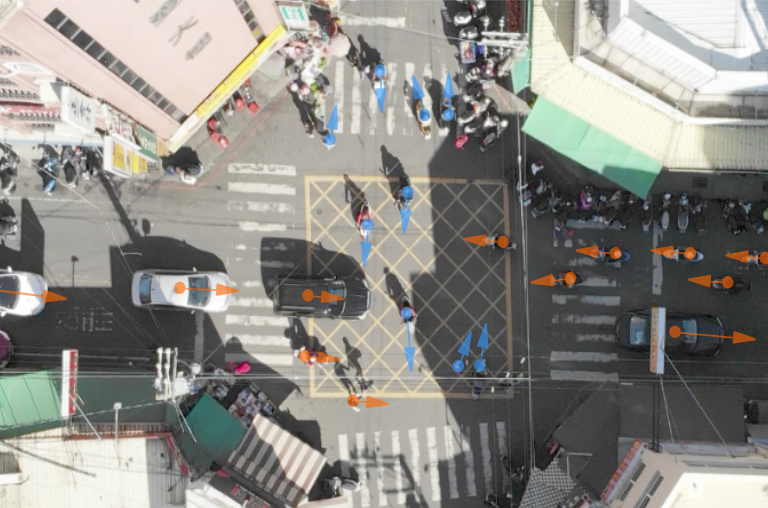
\includegraphics[scale=0.8]{complex_intersection_mod_demo.png}
\end{center}
\caption{A crossroad with no signal.}
\label{INTERSECTION} 
\end{figure}

The main reason for autonomous vehicles being potential threats to other road users is that they do not understand the meanings behind human behaviors and can not foresee their intentions. According to the report by the state of California Department of Motor Vehicles (DMV), 18 of the 33 filed accidents with autonomous vehicles in 2019 (as of June 17, 2019) are rear-ended\cite{CADMV}. Most accidents (over 60\%) happened as autonomous vehicles yielded unnecessarily for situations that following human drivers apparently did not anticipate. Autonomous vehicles are designed to drive conservatively for the cause of safety, but when those behaviours are not understandable to human drivers, over conservative autonomous vehicles become a new threat.

%%%%%%%%%%%%%%%%%%%%%%%%%%%%%%%%%%%%
%%  How interactions are studied  %%

To prevent the problem addressed, interactions with surrounding agents should be achieved by understanding their behaviors. Decisions based on purely control logics such as traditional collision avoidance systems suffer from insufficient reaction time as reported in \cite{Coelingh2010}. To warn drivers early enough to take proper actions, behavior prediction models are used, for example see  pedestrians predictions in \cite{Bonnin2014, Schneemann2016, HASHIMOTO2016}. In these studies, pedestrian crossing intentions are identified and modeled, making their behaviors comprehensible and thus greatly improve the safety of road users. Driver behaviors are also crucial for making safe decisions in traffic flow \cite{Ramyar2015, Gadepally2014}.
%%%%%%%%%%%%%%%%%%%%%%%%%%%%%%%%%%%%

Although modeling human intentions have been the focus of several existing studies, these models are however based on either extensive data collections that are difficult to adapt to new environments or implicit model framework that are intractable for on-line application. We study driver behaviors at unsignalized crossroads and build explicit probabilistic models in this work. Proper behavior model should enable computer drivers to understand and to interact with human drivers more smoothly, resulting in a safer human-computer mixed traffic flow. In what follows, we reviewed driver models in Section 2; our proposed probabilistic driver behavior models in unsigalized crossroads are presented in Section 3; Section 4 provides extensions of the driver model on some real world applications; Section 5 concludes the study with future work. 

% The primary goals as well as the process for the model construction are listed as follow:

% \begin{enumerate}

%     \item \textbf{Identification of driver decision making process} \\
%         How human drivers perceive and react to the traffic participants at the crossroad will be identified.
        
%     \item \textbf{Driver behaviors modeling}\\
%         Based on the current states of the target driver, a behavior model will be constructed based on the decision making process learned previously.
        
%     \item \textbf{Case study}\\
%         Possible applications using the proposed driver behavior model will be explored.

% \end{enumerate}




\chapter{Background and Literature Review}
\label{chap:Lit}

%%%%%%%%%%%%%%%%%%%%%%%%%%%%%%%%%%%%
%{Background and Literature Review}%
%%%%%%%%%%%%%%%%%%%%%%%%%%%%%%%%%%%%

%{summary for all the literature review}

%{ classification of motion models }
Motion planning for autonomous vehicles has been studied extensively to provide optimal and collision-free trajectories\cite{motion_planning}. Most algorithms assume known trajectories of all surrounding agents, while in fact we have very limited information about  vehicles around us. Predicting surrounding vehicles' movements enables more active and more practical traffic studies. In the following section, based on the method employed, motion prediction models are classified into three main categories, namely physics-based models, driver behavior models and interactive models.

%Without in-traffic direct communications or high-level traffic commands, existing assumption is not realistic. 

\subsection{Physics-Based Models}
\label{Literature:Physics-Based}
Physics-based motion predictions use dynamic or kinematic models governed by simple physics laws as surveyed by Lef{\`e}vre et al. in \cite{survey_motion_prediction}.  These physics-based models predict the possible motion of the surrounding agents adopt  linear-velocity models for their efficiency, friendiness in use, and good accuracy in short-term predictions\cite{physics_real_time, physics_velocity_obstacle}. However, they do not account for uncertainties in real traffic with other human drivers. Zhan et al. use  probability models of yielding/passing actions at a crossroad\cite{non-conservative}. Other prediction models such as the work of Ruf et al. \cite{sparc} use a cost map with probabilistic values on each path to optimize the global planner of vehicle movements. Although physics-based models are easier and cheaper to be applied, they suffer from poor long-term predictions, therefore have little interactions between the ego vehicle and other agents.

% \begin{figure}[htbp]
% \begin{center}
% 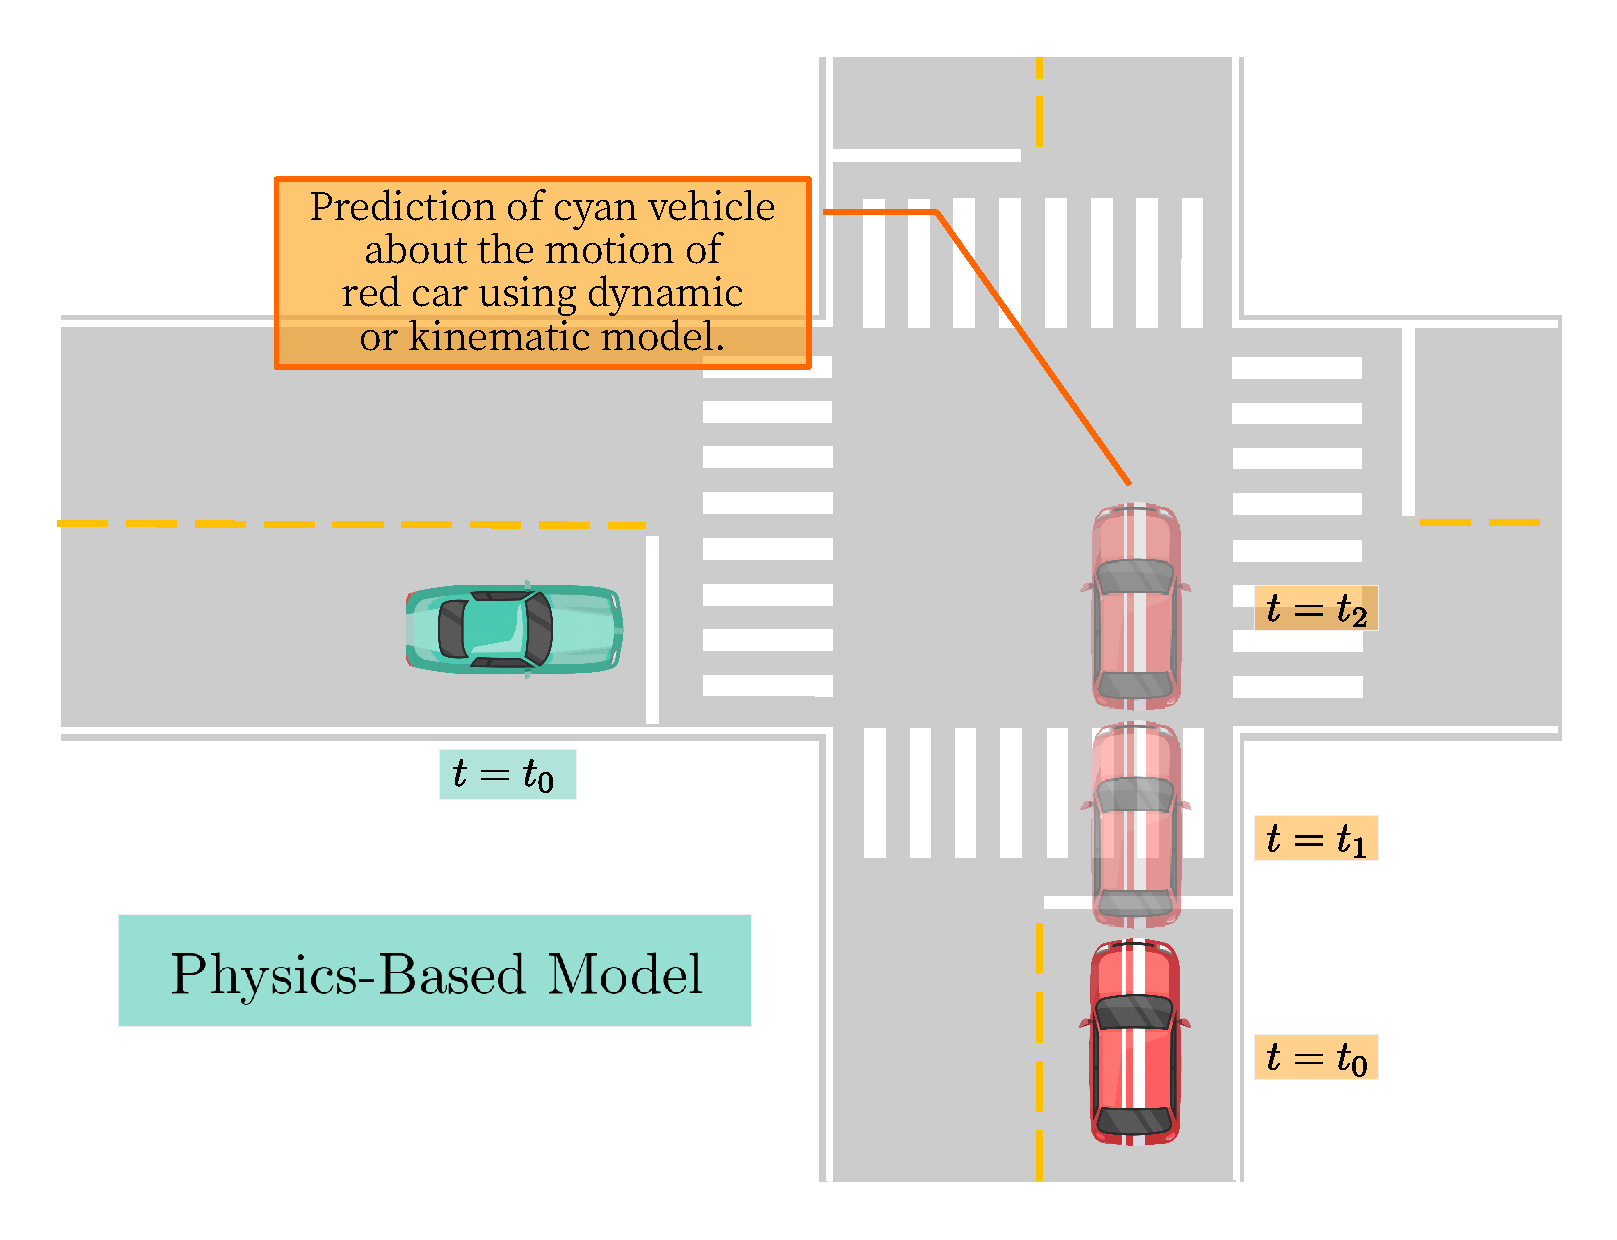
\includegraphics[scale=0.3]{intersection_physics.pdf}
% \end{center}
% \caption{Physics-Based Model.}
% \label{physics-based} 
% \end{figure}


\subsection{Driver Behavior Models}
\label{Literature:Driver Behavior}
Motion predictions with driver behavior models on gas pedals/braes/steers along a path are the intent recognition processes based on the previous and current states of the target agents. Possible behaviors of surrounding agents are listed with a likelihood measure such as Bayesian networks or hidden Markov Model (HMM). Such models can be used, as an example, to estimate the chance of a vehicle violating a stop sign with dynamic Bayesian network (DBN) without extensive trajectory predictions \cite{Lefevre2012}. Dagli et al. \cite{Dagli2003} used the same concept in building vehicle following and lane changing models with sensor data uncertainty as well as uncertainties in human behaviors. Their study is assessed in simulated lane changing experiments where the driver behaviors is recognized 1.5 seconds earlier than the actual lane change. Gindele et al. \cite{Gindele2013} use DBN, combined with the manually formulated models and models learned with random forest tree,  to estimate and predict the driver behaviors of two cars passing an intersection. 

%Online learning is possible in the proposed method where the model would be able to adapt to new environments.

% \begin{figure}[htbp]
% \begin{center}
% 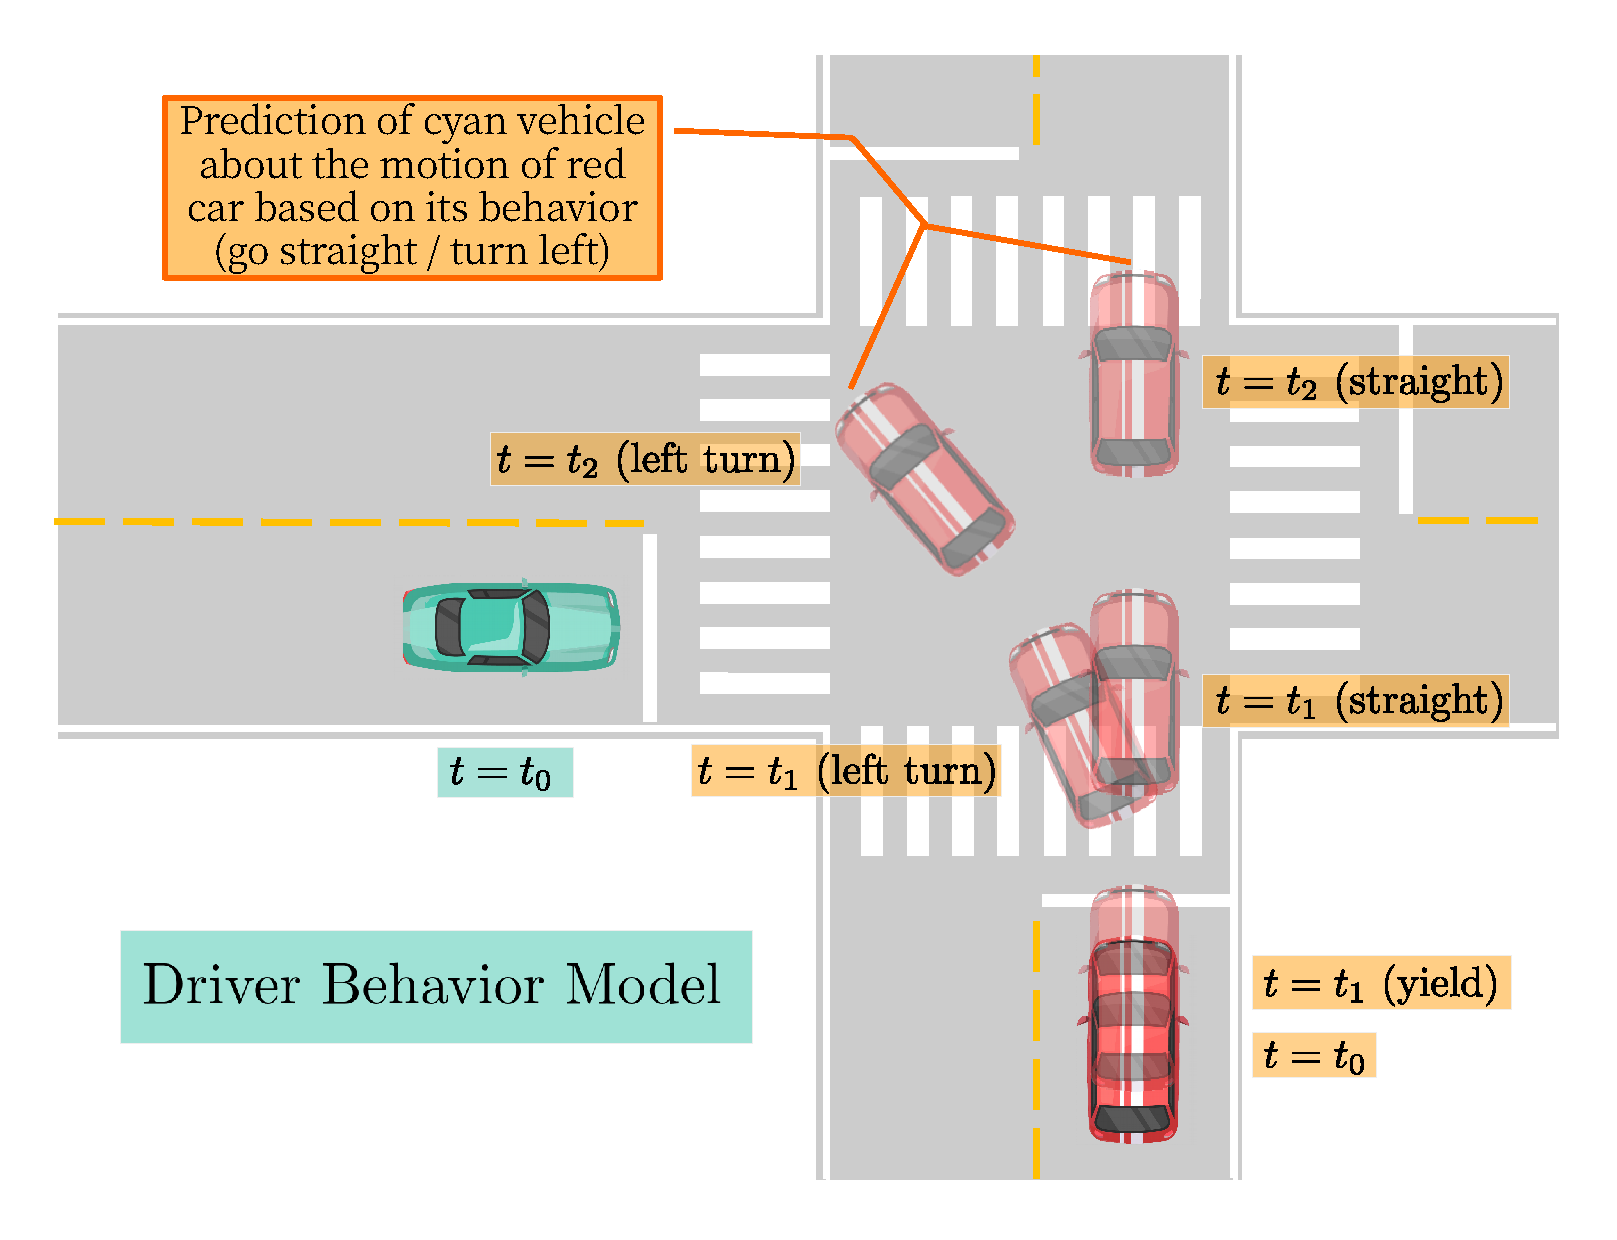
\includegraphics[scale=0.3]{intersection_behavior.pdf}
% \end{center}
% \caption{Driver Behavior Model.}
% \label{driver_behavior} 
% \end{figure}


\subsection{Interactive Models}
\label{Literature:Interactive}
Long-term predictions have been achieved using interactive models with other agents. For example, at a vehicle might decide to pass an intersection because he/she believes that other vehicles are very likely to brake. Probabilistic methods such as partially observable Markov decision process (POMDP) have been used as the core of interactive models to determine the actions of an ego vehicle by predicting the future states of other agents. Foka et al. use FOMDP to navigate in a space with obstacles in \cite{Foka}. Hubmann et al. use POMDP to evaluate the possible maneuvers of other agents and optimize the actions of the ego vehicle in \cite{state_uncertain_environment}. However, POMDP is computationally expensive and therefore unable to be used for  real-time predictions. In addition, vehicle drivers need to predict the trajectories of only nearby vehicles, instead of all, a downsized POMDP application with only nearby vehicles is needed.

% \begin{figure}[htbp]
% \begin{center}
% 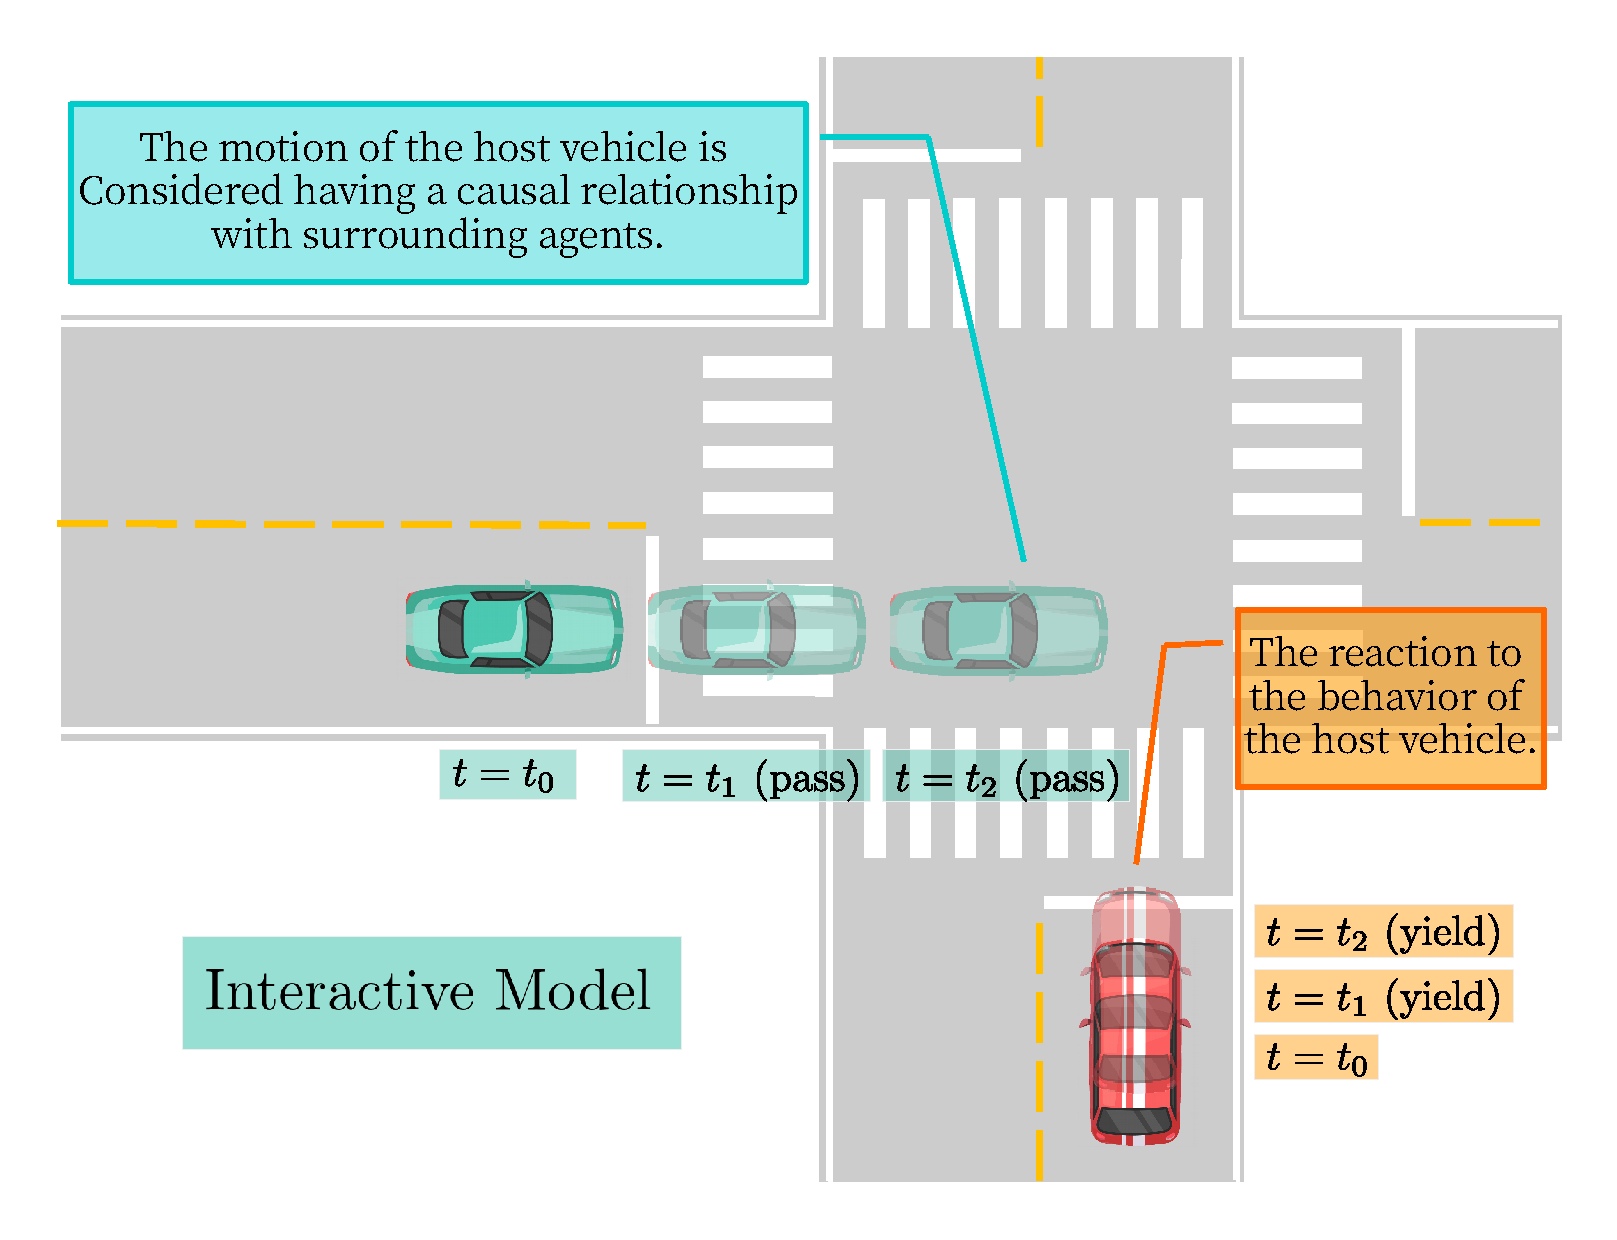
\includegraphics[scale=0.3]{intersection_interactive.pdf}
% \end{center}
% \caption{Interactive Model.}
% \label{interactive} 
% \end{figure}



\subsection{Explicit Driver Behavior Models}

Behavior models provide driver intent for predictions in urban intersection that form the basics for current advance driver assistance systems (ADAS). Liebner et al. use intelligent driver models (IDM) for probability of turning and car-following behaviors in a simple Bayes net in \cite{Liebner2012} with different intention probabilities in arbitrary intersections with general speed profiles. To overcome driver behavior change, the features of different agents, such as speed, distance to the intersection, are extracted by Graf et al. in the process of case-based reasoning (CBR) for site-specific intersections\cite{Graf2014}. CBR relates a case with similar experiences to predict the behavior of the driver. However, the results learned from one intersection still may not directly applicable for other intersections. Drivers with different driving style also affect the prediction accuracy significantly.   

\subsection{Summary}
Despite the explicit formulation and general applicability, physics-based models can not account for states changes of the subject, which results in the poor long-term prediction. Interactive models with joint behaviors of surrounding agents could achieve better long-term predictions, with the sacrifice of  computational cost and unable to handle large state spaces. Driver behavior models, on the other hand, have better long-term estimations than physics-based models \ref{Literature:Physics-Based} and better computational efficiency than interactive models \ref{Literature:Interactive} trained models are, however, only applicable to environments where the training data are extracted. More general and explicit driver behavior models at various traffic scenarios are needed to smoothly blend into urban traffic with mixed fleet. Each driver needs to understand the behaviors and intentions of other road users so that they can and react accordingly. 

Autonomous vehicles nowadays do have the ability to resolve some potential threats, actively maneuver vehicles to avoid obstacles; however, they usually do so with no regard of what the maneuvers are perceived by human drivers. While technology can observe what's going on based on captured evidences, intentions are more subtle than behaviors. Human drivers can pass the interactions by predicting the intention of the other agents : accelerate to pass or decelerate to yield. Since humans don't perceive the world numerically, researchers have suggested that instead of calculating the distance and the speed directly to learn the time to hit an object, human drivers adopt a more cognitive and abstract methods \cite{cog}.

In this work the driver behavior models is chosen for its better long-term prediction and computational efficiency compared to the other two models.  Hence, in the following chapters, an explicit driver behavior models will be developed to account for driver behaviors at various traffic scenarios.


 
\chapter{Human Driver Modeling at Crossroads}
\label{chap:DriverModel}
\resetfigpath{Chap3}

%%%{INTRODUCTION to this CHAPTER}%%%
When we are driving, unless no other traffic participants nearby, interactions between drivers happen much more frequent than we realize. Autonomous vehicles, or computer driven vehicles, nowadays are quite adept at driving between lines, make a turn or avoid an obstacles. They are also capable of reacting to humans' behavior, but more often than not, those reactions are not what we expected. This is owing to their incapability of interacting with human. Autonomous vehicles can't communicate with us if they can't understand our gesture or how we usually react to some specific situation. To solve this, we need to develop a model that is able to account for human driver behaviors. The unsignalized crossroads is chosen as the scenario that the model build around for the fact that it is the most communication-requiring traffic scenario, where the other participant's intention to pass or yield is required.

In the following sections, the concepts of time to collision and time for action will be introduced in Section ~\ref{sec:TTCandTFA}. Time to collision and time for action are both key elements for the proposed method, which define the mechanism drivers employed to avoid the potential collision from happening. In Section ~\ref{sec:TFADistribution}, time for action is transformed into a distribution to estimate the chance of braking, and based on this idea, a probabilistic evaluating model is proposed in Section ~\ref{sec:POY}. Finally, to verify and validate the proposed model, experiments at both simulated and real crossroad are conducted in Section ~\ref{sec:ValidatePOY}.


%%%%%%%%%%%%%%%%%%%%%%%%%%%%%%%%%%%%%%%%%%%%%%%%%%%%%%%%%%%%%%%%%%%%%%%%
%%%%%%%%%%               SECTION SECTION SECTION               %%%%%%%%%
%%%%%%%%%%%%%%%%%%%%%%%%%%%%%%%%%%%%%%%%%%%%%%%%%%%%%%%%%%%%%%%%%%%%%%%%

\section{Time to Collision and Time for Action}
\label{sec:TTCandTFA}
When crossing an unsignalized crossroad, the longitudinal speed is decided empirically by human. Drivers observe the oncoming vehicle in a short amount of time and estimate the next possible position, speed and direction it might be, mostly by experience. Then the speed is adjusted accordingly: accelerate to pass the vehicle if drivers \textbf{believe} that arrive at the crossroad before the other participant is possible; or decelerate to yield if a collision is anticipated. Since humans don't perceive the world numerically, researchers have suggested that instead of calculating the distance and the speed directly to define the time to hit an object, more cognitive and abstract methods are used \cite{cog}. In this section, we first introduce the crossroad model. Then, to make driver behavior predictable for computer driven vehicle, researches regarding such mechanism are studied and applied. Finally, a probabilistic model of driving behavior is then developed.

%%%%%%%%------------------------------%%%%%%%%%
%%%%%%%%-----------SUBSECTION---------%%%%%%%%%
%%%%%%%%------------------------------%%%%%%%%%
\subsection{Crossroad Modeling}
\label{sub:crossroad}
A crossroad model where the whole scenario based on is introduced before digging deeper into the driver decision mechanism at the crossroads. Fig.~\ref{fig:model_demo} illustrates a human driver (on the left, heading to the right) and an autonomous vehicle (on the bottom heading upward) crossing a perpendicular crossroad with no signal. Under this circumstance, to reduce the dimensionality of the state space, only on the longitudinal states of concerning vehicles are considered. Also, to prevent confusions, only the interactions between two vehicles are studied at the beginning. In this scenario, \textbf{\emph {the node}} represents the intersection of the extended lines of movement of two traffic agents and would be represented by the symbol like the node in figure Fig.~\ref{fig:model_demo}. 

\begin{figure}[t]
\begin{center}
%\setlength{\unitlength}{0.012500in}
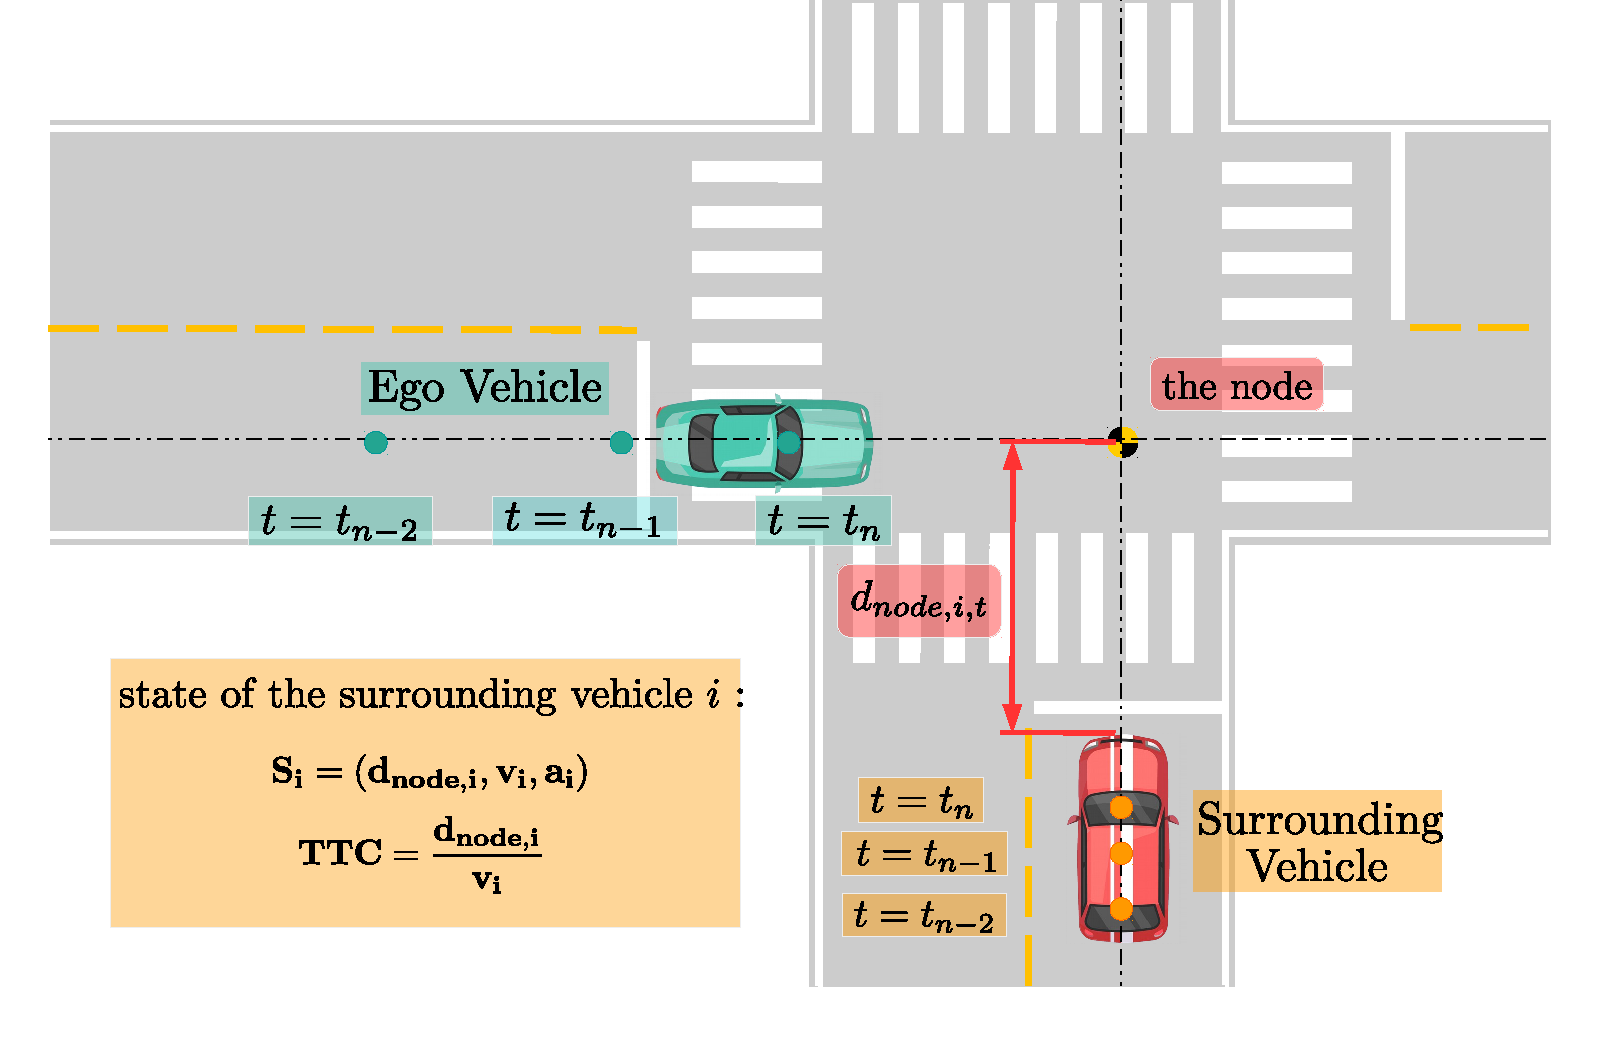
\includegraphics[scale=0.5]{intersection_concept.pdf}
\end{center}
\caption{Demonstration of the proposed scenario and relevant variables.}
\label{fig:model_demo} 
\end{figure}

the node is used as the origin of the coordinate system. The positive $x$ direction is same as the vector of velocity of the first approaching vehicle, and positive $y$ direction as the vector of velocity of the other vehicle. The state of the $i~\text{th}$ vehicle is defined as : 

\begin{equation}
\mathbf{S}_{i,t} = \left( \begin{array}{c} \mathbf{d_{node}}_{i,t} \\ \mathbf{v}_{i,t} \\ \mathbf{a}_{i,t} \end{array} \right), \mbox{ where }  i=\{0, 1, 2, ..., N\} 
\label{eq:state}
\end{equation}

\noindent where $d_{node, i, t}$ is the displacement from the position of the $i~\text{th}$ vehicle to that of the node, $v_{i, t}$ and $a_{i, t}$ are the speed and the acceleration of the $i~\text{th}$ vehicle at time $t$ respectively. Given that $\mathbf{S}_{0}$ is the state of the ego vehicle, $N$ is the number of its surrounding vehicles. Note that they are all one-dimensional. 


As mentioned previously, the main purpose is to find out how human drivers interact with the other moving vehicle as he or she proceeds towards the the node. To focus on this topic, the crossroad model is simplified : only one lane per direction, and one participant driving on each direction. As a consequent, the maneuvers of drivers are reduced to linear motion involving hitting the braking and the gas pedal.  In the following section, the resulting crossroad model is used to determine the mechanism behind the decisions making process of potential collision avoidance.



%%%%%%%%------------------------------%%%%%%%%%
%%%%%%%%-----------SUBSECTION---------%%%%%%%%%
%%%%%%%%------------------------------%%%%%%%%%
\subsection{Time to Collision}
\label{sub:TTC}

How human decide when is the moment to start braking to avoid collision with a stationary obstacle or another moving vehicle has been a popular topic since a couple decades ago \cite{Caird1994}. \ac{TTC}, or time to contact, is a crucial method for human to predict the time it will take to reach the obstacle and take necessary measure to prevent potential collisions from happening. Being an efficient safety measure in traffic safety assessment for decades, TTC was described as “the time required for two vehicles to collide if they continue at their present speed and on the same path.” by Hayward in \cite{Hayward1972}. This concept was usually applied to deal with car following problem, but in this research, it is used to handle vehicle interactions at the crossroad.

The original definition was specified by an optic variable $\tau_{optic}$ ,which is the inverse of the rate of dilation of the object relative to the observer as shown in Eqn.~(\ref{eq:TTC_tau}). 

\begin{equation}
TTC = \frac{\theta_1}{(\theta_2 - \theta_1)/(t_2 - t_1)}
\label{eq:TTC_tau}
\end{equation}

In the Eqn.~(\ref{eq:TTC_tau}), $\theta_1$ and $\theta_2$ are the angular distances of the obstacle's image on the retina at times $t_1$ and $t_2$ separately. Hence the $(\theta_2 - \theta_1)/(t_2 - t_1)$ would be the expansion rate of the obstacle as the observer approaches. However, there are intense disputations over whether $\tau_{optic}$ provides necessary TTC information, since both empirical results and analyses suggest that the hypothesis is false, as described in \cite{tau}. 

There also exist another potential way to describe TTC involving the information of the speed and the distance to the target object, as described in Eqn.~(\ref{eq:TTC_dv}).

\begin{equation}
TTC = \frac{\text{distance to obstacle}}{\text{speed}}
\label{eq:TTC_dv}
\end{equation}

Also known as cognitive or computational strategy, this method takes account of the distance from the obstacle (the target object) and the speed assessed by the driver. To verify this idea, Cavallo et al. \cite{TTC} conduct a series of experiments in real driving condition. Volunteers of different ages, genders and experience levels in driving were asked to estimate the time it would take to collide with the obstacle. The results suggested that both speed and distance information are taken into account in TTC estimation. 

Since the TTC definition in Eqn.~(\ref{eq:TTC_dv}) is more applicable and also verified in the literature, in this research the speed and the distance to the intersection are used as variables to describe the human driver behaviors in proposed model. 


%%%%%%%%------------------------------%%%%%%%%%
%%%%%%%%-----------SUBSECTION---------%%%%%%%%%
%%%%%%%%------------------------------%%%%%%%%%
\subsection{Time for Action}
\label{sub:TFA}

TTC provides a way to imitate the method used by human drivers when facing a potential collision event. However, the goal is to predict the other participant's decision, that is, to pass or to yield, and the mechanism of this decision is still unclear. To explain the decision making process, we will introduce the new term "\ac{TFA}".

To fully understand the role of TFA in braking decision, first the definition of TTC is used to explain how the braking decision is made : under a given speed, the driver decides to brake to avoid collisions when a certain distance is left between the car and the obstacle. As shown in Fig.~\ref{fig:TTC_history}, a car is approaching from the left while a red obstacle is on its path. At point $P_A$, the car is cruising with constant speed $V_0$. The driver should have already observed the obstacle but he or she feels no pressure to brake at this point. As the car keeps moving forward, the driver realizes that if he or she does not brake here, the vehicle might collide with the red obstacle. After the brake being applied at $P_B$, the car begins to slow down and finally comes to a stop with the speed equals to $0$ at point $P_C$. 

In this scenario, TTC decreases as the distance to the obstacle is getting shorter. Finally at point $P_B$, the driver decides to brake to keep a safe margin from the vehicle to the obstacle when the car is fully stopped. The distance from point $P_B$ to the obstacle is the "distance left before action", which is the minimum distance required to stop in front of the obstacle and keep the safe margin in between. Now we divide this distance by the speed at point $P_B$, we get this TTC where the driver take the action to avoid the collision. We call this TTC "Time for Action (TFA)". 

The time-history of TTC and the dependent variables depicted in Fig.~\ref{fig:example_TTC_TFA} are put together and presented in Fig.~\ref{fig:TTC_history}. The figure used here is similar to the time-history of braking presented in the work of Winsum et al. \cite{time_history}. The motion of the vehicle cruising from point $P_A$ to $P_B$ in Fig.~\ref{fig:example_TTC_TFA} results in the TTC drops from $t=0$ to $t=t_0$ in Fig.~\ref{fig:TTC_history}. This is due to the decrease of the distance to the obstacle while the speed of the vehicle is constant. Then the driver brakes at point $P_B$ in Fig.~\ref{fig:example_TTC_TFA} as the driver brakes at time $t_0$ in Fig.~\ref{fig:TTC_history}. 

\begin{figure}[htbp!]
\begin{center}
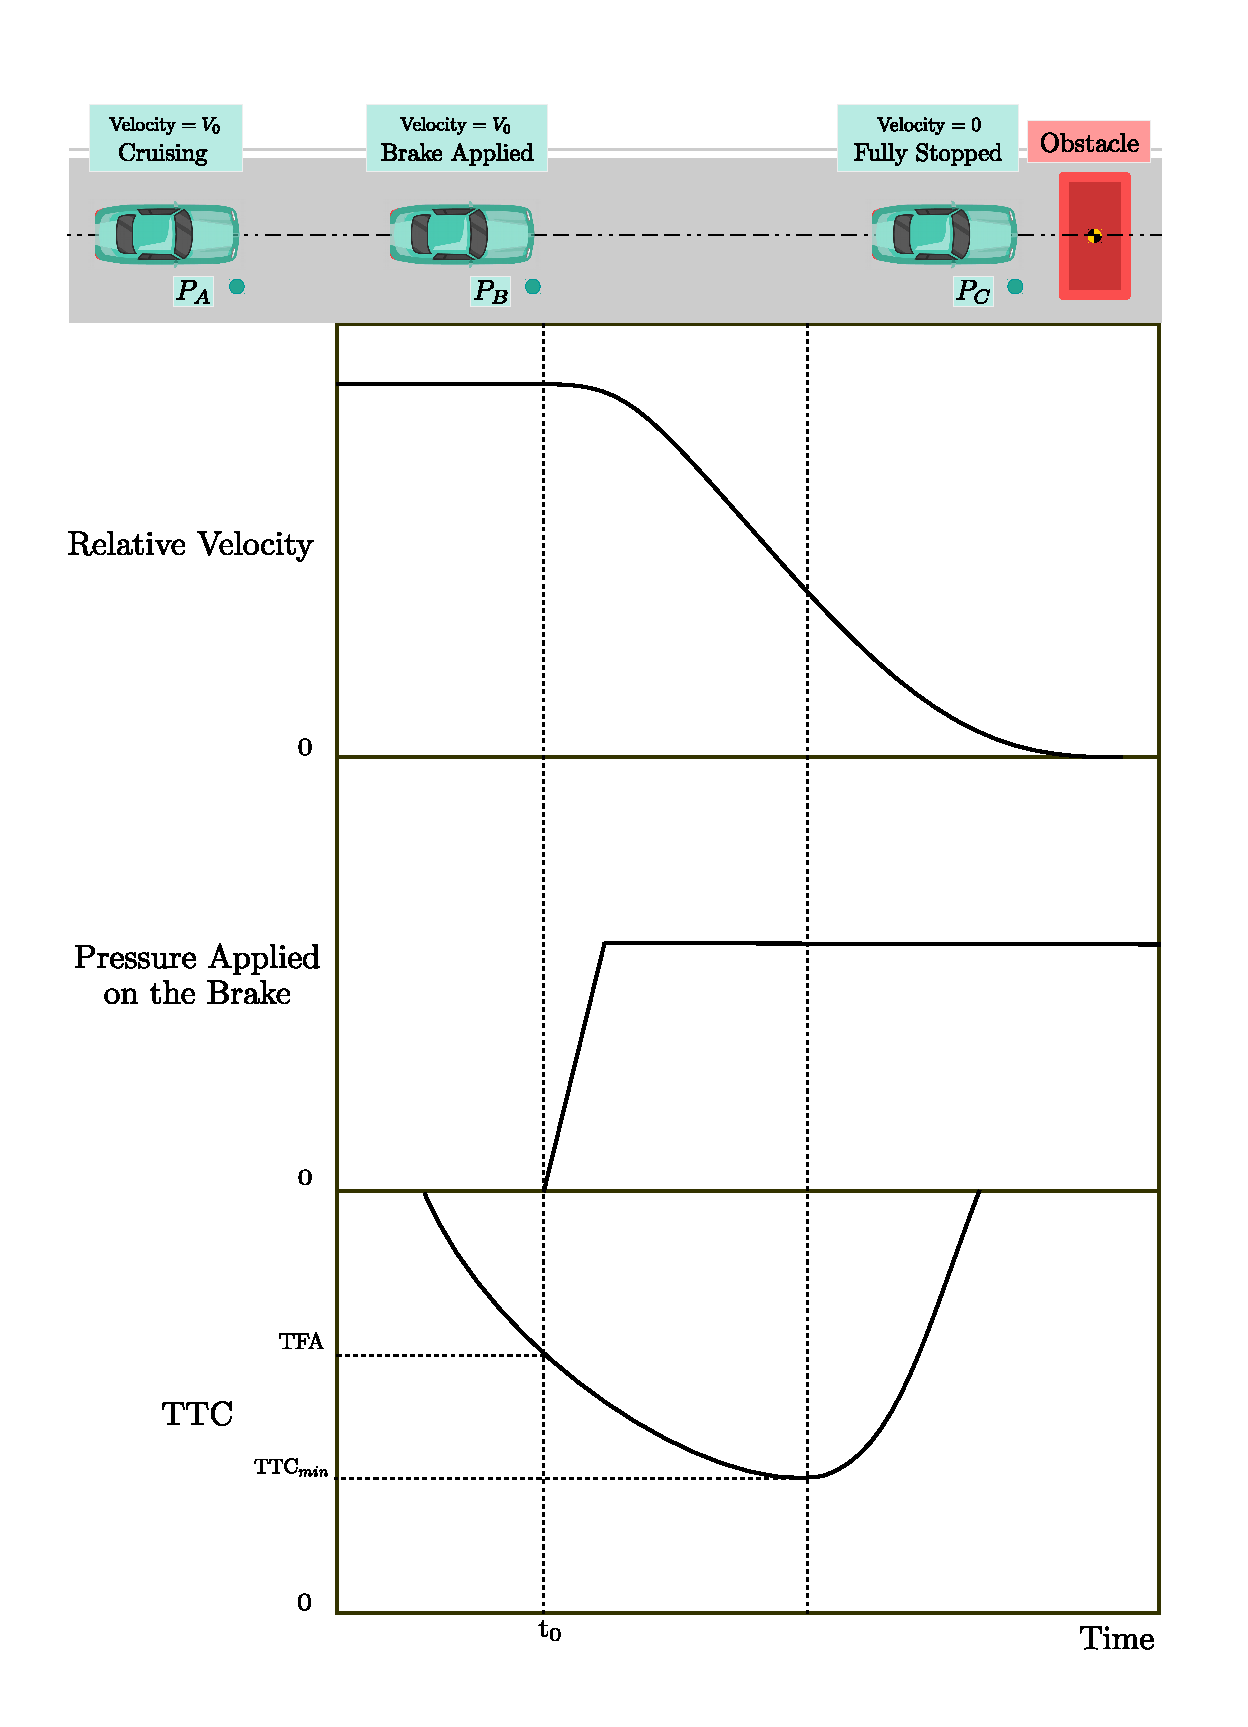
\includegraphics[scale=0.63]{TTC_change_when_braking.pdf}
\end{center}
\caption{History of time to collision when brake is applied.}
\label{fig:TTC_history} 
\end{figure}

The TTC value at this instance should equal to TFA of the driver under this speed by definition since this is the TTC he or she believes that a collision would happen if the brake is applied any later. During the braking, TTC drops to its lowest point labeled as $TTC_{min}$ and then rises. The rise is due to the the speed decreasing rate (i.e. acceleration) being higher than the rate of the distance decrease (i.e. the speed). Note the TFA is the minimum TTC that drivers start to hit the brake to avoid collision, not the minimum TTC during the whole process (which is the $TTC_{min}$ in Fig.~\ref{fig:TTC_history}).

From the above paragraph we know that not solely speed or distance is utilized in the decision of braking, it is the TTC which formulated using the combined information of both variables that driver perceived take parts in the mechanism. In the crossroad scenario, when a vehicle is about to arrive at the crossroad at the same time as the host vehicle, the host vehicle driver subconsciously imagines the future position of the oncoming vehicle, which turns out to be a real obstacle exist at the point of intersection due to the fact that the only location of the potential collision is at the intersection of two perpendicular paths (as shown in Fig.~\ref{fig:imagine_obstacle}). Despite there is not really an obstacle lying right in the middle of the crossroad, we tend to prevent the worst case from happening by estimating the next possible position of the oncoming vehicle with the tangential path. We can adjust our speed accordingly to avoid the potential collision.  

\begin{figure}[htbp!]
\begin{center}
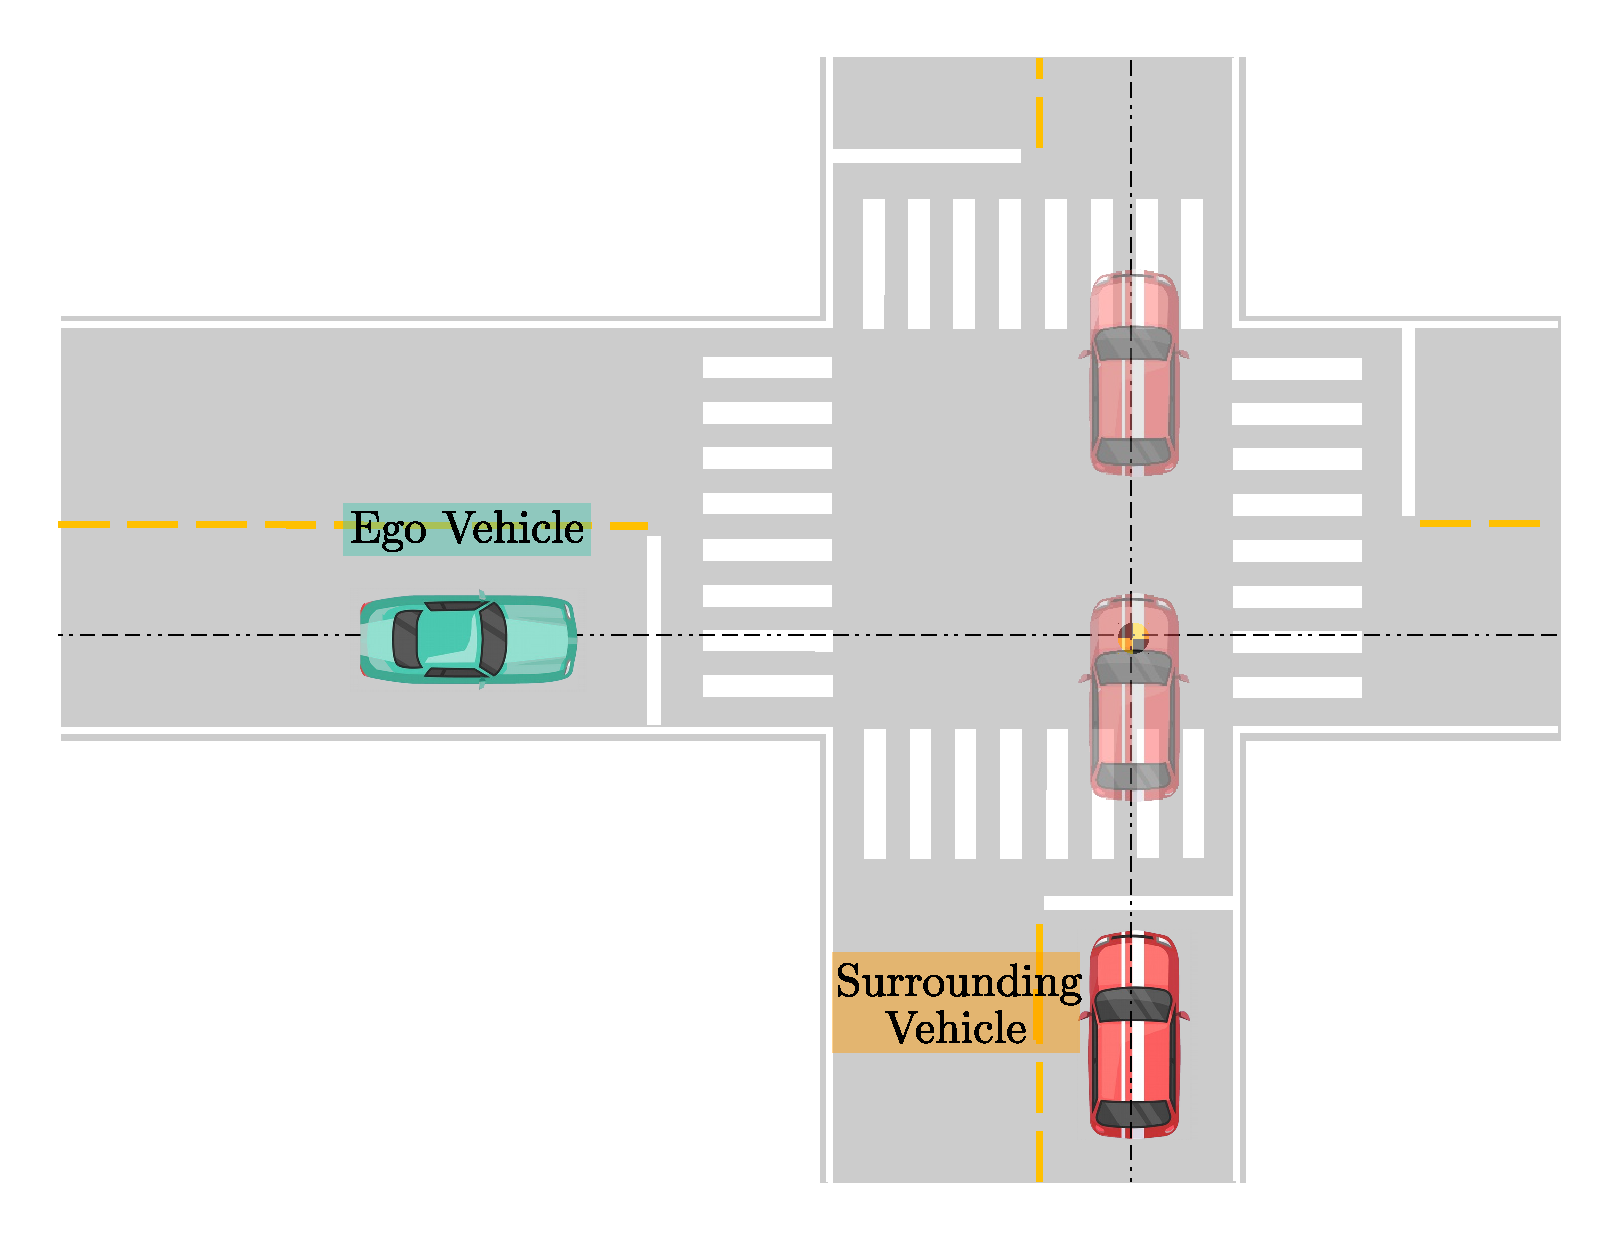
\includegraphics[scale=0.43]{intersection_imagining_obstacle.pdf}
\end{center}
\caption{The host driver estimate the possible position of the oncoming vehicle depending on its current states. To avoid the potential collision, the host driver adjust the time to brake as if the oncoming vehicle is at the intersection.}
\label{fig:imagine_obstacle} 
\end{figure}

Now let us bring TTC and TFA into our crossroads scenarios. Since TTC here can be estimated using the distance to the intersection and the current speed of the vehicle while the TFA is the same as in the situation which a real obstacle exists at the intersection, combining Eqn.~(\ref{eq:state}) and Eqn.~(\ref{eq:TTC_dv}) we have : 

\begin{equation}
\mathbf{TTC} = \frac{\mathbf{d_{node,i}}}{\mathbf{v_{i}}}
\label{eq:TTC_crossroad}
\end{equation}

In this case, at the moment the host driver sees the oncoming vehicle and thinks that it might collide with him, he or she would put the foot on the brake while the TTC is dropping. Then, the brake would finally be applied at the instance that the TTC he cognized is equivalent to his TFA, so the potential collision at the node (the intersect of two routes) would be avoided. Note that the $\mathbf{d_{node,i}}$ here represents the \textit{displacement} instead of the distance for the purpose of distinguishing two opposite sides of the node, in other words, the displacement is adopted to separate the states before and after passing the node. So, the direction the host vehicle faces would always be the positive on the coordinate system. Throughout this research, the use of displacement and distance are interchangeable since the situations that we are interested in happen before the node (i.e. the displacement is always positive).



It is clear until now that the particular moment of decision making at the crossroad is accessible if both TTC and TFA are able to be determined. The TTC can be calculated without effort by dividing the displacement to the node by the speed of the subjective vehicle. However, there is little discussion about the concept of TFA in the literature. Also, even if the access to the very TFA of the driver is possible, which in fact only an approximated value could be acquired, it is still not guaranteed that the driver will hit the brake at that exact moment since the randomness of the human perception and the resulting errors while generating the actions. This issue will be addressed thoroughly in the following section.

In the previous sections, the literature concerning psychology and cognitive science is investigated to determine the deciding component (i.e. TTC and TFA) in human drivers' braking event. Then, both variables are applied in the crossroad scenarios as illustrated in ~\ref{sub:crossroad}. In the next section, an assumption that is capable of explaining the stochastic character of TFA will be established. Then a probabilistic model of drivers behavior based on the concepts of TTC and TFA will be proposed to handle the stochastic decision process of human at the crossroad. 


%%%%%%%%%%%%%%%%%%%%%%%%%%%%%%%%%%%%%%%%%%%%%%%%%%%%%%%%%%%%%%%%%%%%%%%%
%%%%%%%%%%               SECTION SECTION SECTION               %%%%%%%%%
%%%%%%%%%%%%%%%%%%%%%%%%%%%%%%%%%%%%%%%%%%%%%%%%%%%%%%%%%%%%%%%%%%%%%%%%
\section{ The TFA Distribution}
\label{sec:TFADistribution}
In this section, the concept of TFA distribution is described. TFA distribution is the fundamental idea to this research an it is what the proposed model is built upon. Following this concept, we are able to obtain the probability density function of TFA from which the probability of the vehicle yielding could be determined using the proposed model.

%%%%%%%%------------------------------%%%%%%%%%
%%%%%%%%-----------SUBSECTION---------%%%%%%%%%
%%%%%%%%------------------------------%%%%%%%%%
\subsection{TFA Distribution}
\label{sub:TFA Distribution}

From the above paragraph we know that the definition of TFA is the minimum TTC (or the minimum distance left before braking at the current speed) that drivers start to hit the brake to avoid potential collision.This decision making process will differ from person to person since each of us has our own risk threshold to decide the braking timing. For example, a young driver with a high performance sports car might have a relatively low TFA because of his personality and the great braking performance of the car which allows the driver to go closer before braking. On the contrary, an older driver driving an aged passenger sedan might have a higher TFA since the driver is more cautious and the car requires longer distance to stop.

\begin{figure}[htbp!]
\begin{center}
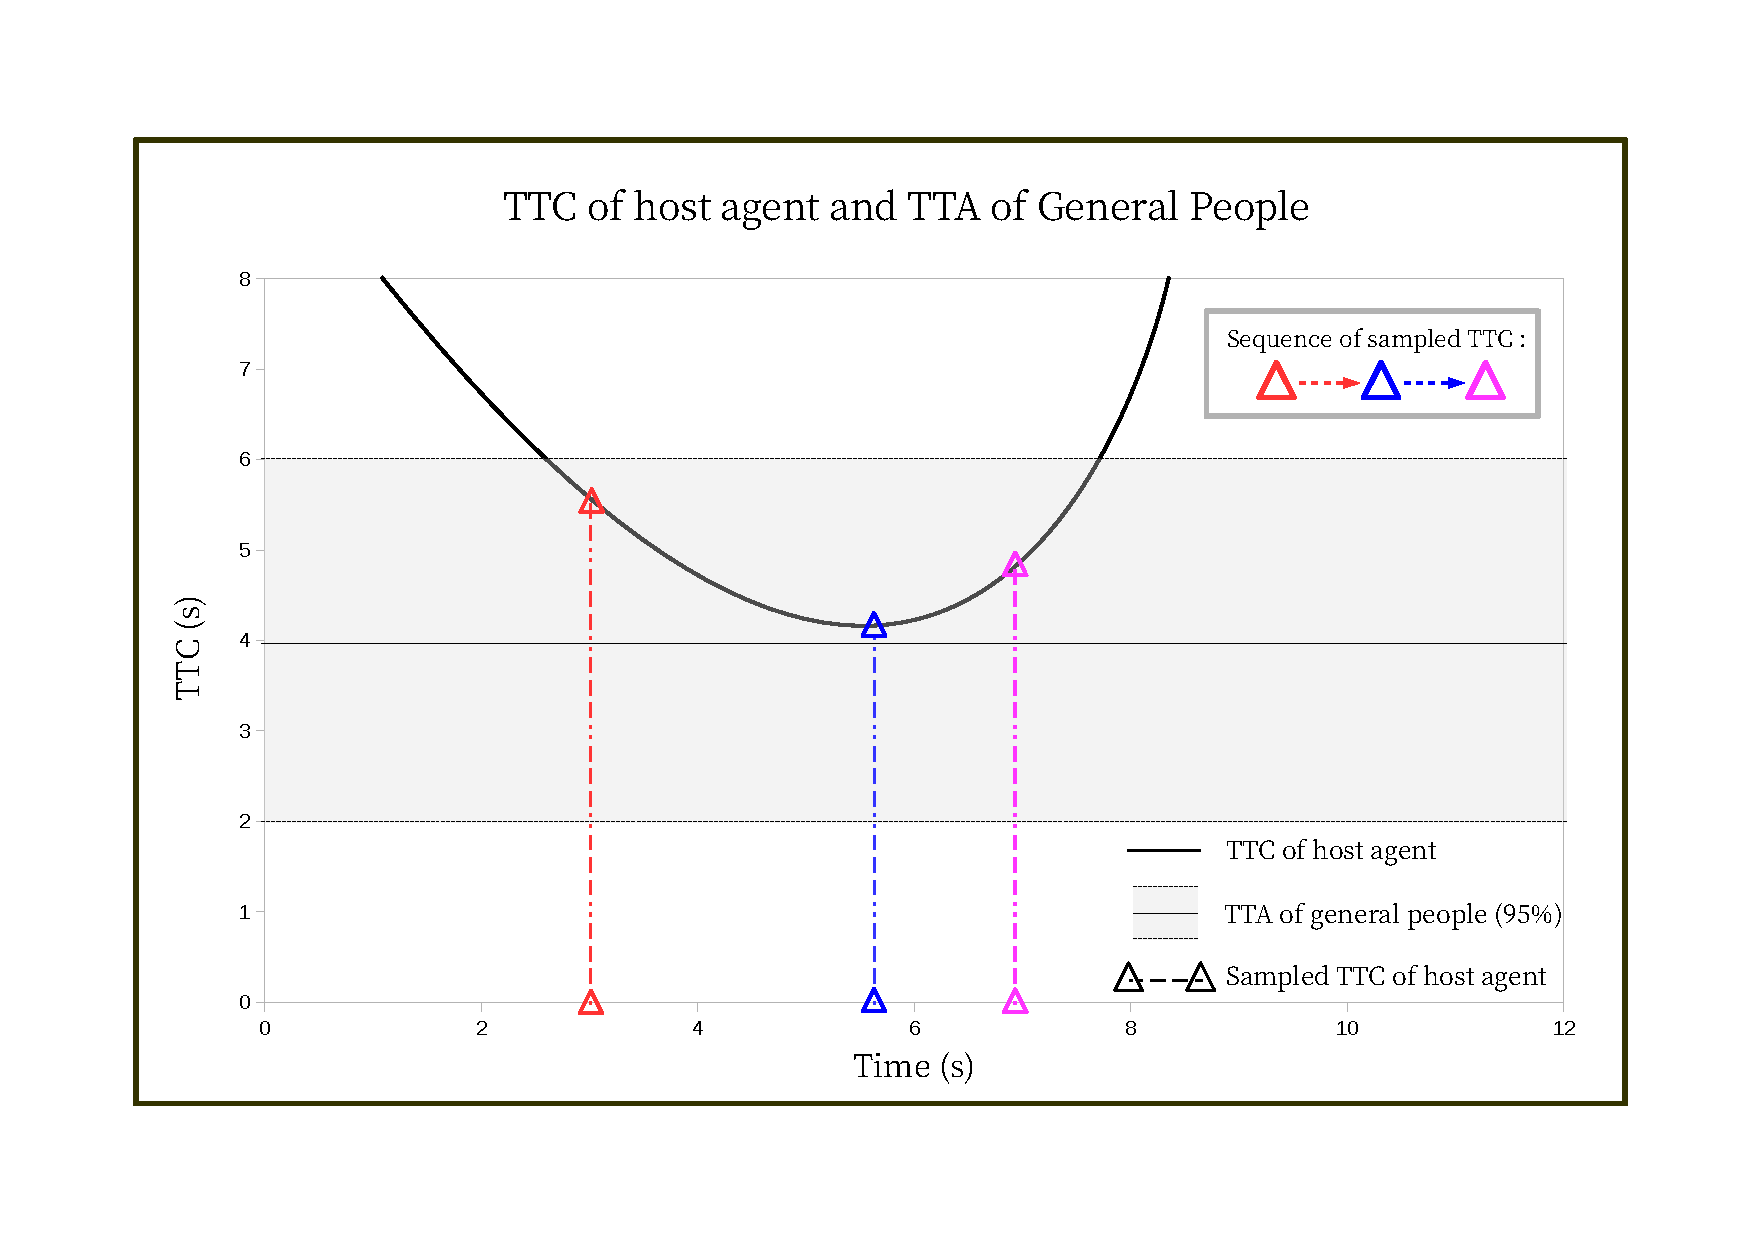
\includegraphics[scale=0.5]{TTC_probability.pdf}
\end{center}
\caption{Example of TFA of general people and TTC of the host agent.}
\label{fig:TTC_TFA} 
\end{figure}

This idea is illustrated in Fig.~\ref{fig:TTC_TFA}. In Fig.~\ref{fig:TTC_TFA}, grey area is drew to illustrate the distribution of TFA of general people (95\% of people's TFAs are within the area) while solid line is indicating the TTC of the host agent changing with time, which is similar to that in Fig.~\ref{fig:TTC_history}. The distribution of TFA can be explained as "within this range of TTC, 95\% of drivers will initiate the action (hit the brake) if potential collisions exist". So in the crossroad scenario where two vehicles are about to reach the intersection at the same time, when the TTC of one of the drivers is getting lower, we can infer that his or her chance of braking to yield is getting higher because more and more people in the distribution start braking as it goes. 

In fact, not only is the TFA of different people a distribution, but the TFA of a person under different personal or environmental conditions also is a distribution. However, there is rarely any literature conducted such experiments, so the assumption that TFA distributions are normally distributed is made. The reason behind this assumption is that even if the distributions of the perception and the motion during the action process (which is braking in this content) are not normally distributed, the combined outcome of these independent random variables would still approximate a Normal distribution, given large enough samples. 

In spite of the fact that this idea is supported by the Central Limit Theorem, experiments are conducted to support the assumption. Both Relative Judgement tasks or Prediction-motion tasks are often employed in the literature to estimate the ability of the participant to derive TTC information . In Relative Judgement tasks, subjects are required to indicate the first arriving moving target from two approaching ones. In the Prediction-motion tasks, on the other hand, subjects are asked to predict the time of the moving object arrive at a specified position after the moving object disappeared from the view. In these tasks, subjects are making decisions while watching a pre-recorded film. 

However, it is hardly possible for subjects to identify the TFA without knowing how the vehicle will response while the brake is applied. Consequently, to make it more similar to the driving scenario in real world, a simulated crossroad environment is constructed. Detailed discussion regarding the simulated crossroad as well as how the experiments are conducted will be delivered in the following sections where model validation is conducted. For now, the focus is put on the distribution of TFA.

In the experiments, three volunteers are asked to drive toward a static vehicle with constant speed and apply the brake when they believe that the collision will happen if it is applied any later. TFAs in this scenario would be the displacement from the host vehicle to the static vehicle divided by speed of the host vehicle at the moment which brake is applied. Results are shown in Fig.~\ref{fig:TFA_distr_1}, Fig.~\ref{fig:TFA_distr_2} and Fig.~\ref{fig:TFA_distr_3}. Noted that the distribution of TFA might varies under different speed, but only the parameters of the distribution are changed, not the type of the distribution. The focus now is on weather the TFA could be modeled as a normal distribution ,the property of TFA distributions under different speed will be discussed later. 

\begin{figure}[htbp!]
\begin{center}
\makebox[0pt]{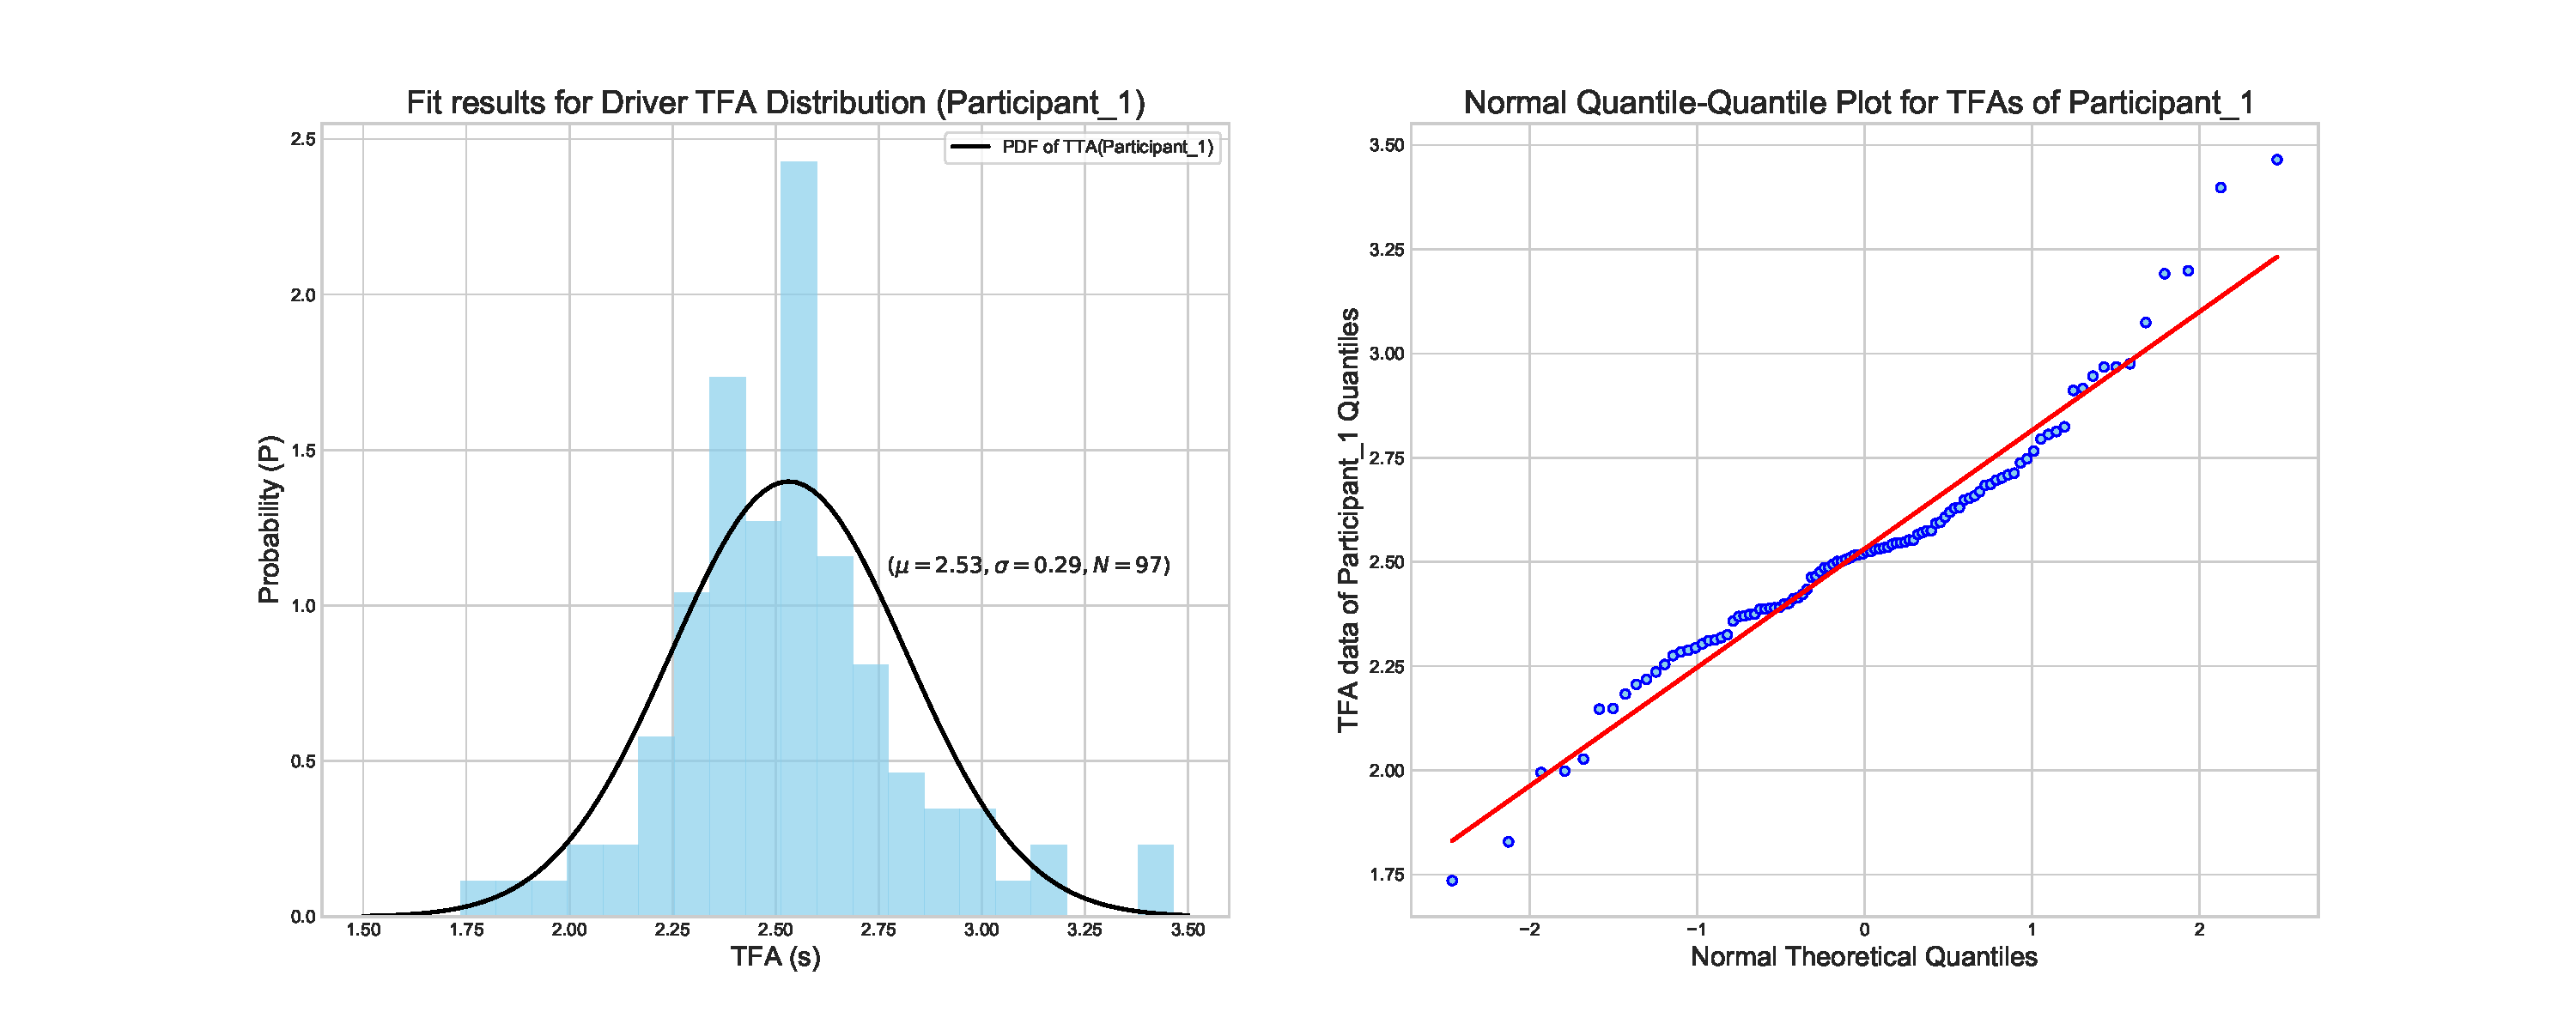
\includegraphics[width=0.8\paperwidth]{Participant_1_0_fitting.pdf}}
\end{center}
\caption{TFA results of participant 1 displayed in histogram. The solid curve is the TFA distribution of participant 1 approximated by Normal distribution ($\mu = 2.35, \sigma = 0.29, N = 97$). Speed of the vehicle while braking was set to 5 m/s. }
\label{fig:TFA_distr_1} 
\end{figure}

\begin{figure}[htbp!]
\begin{center}
\makebox[0pt]{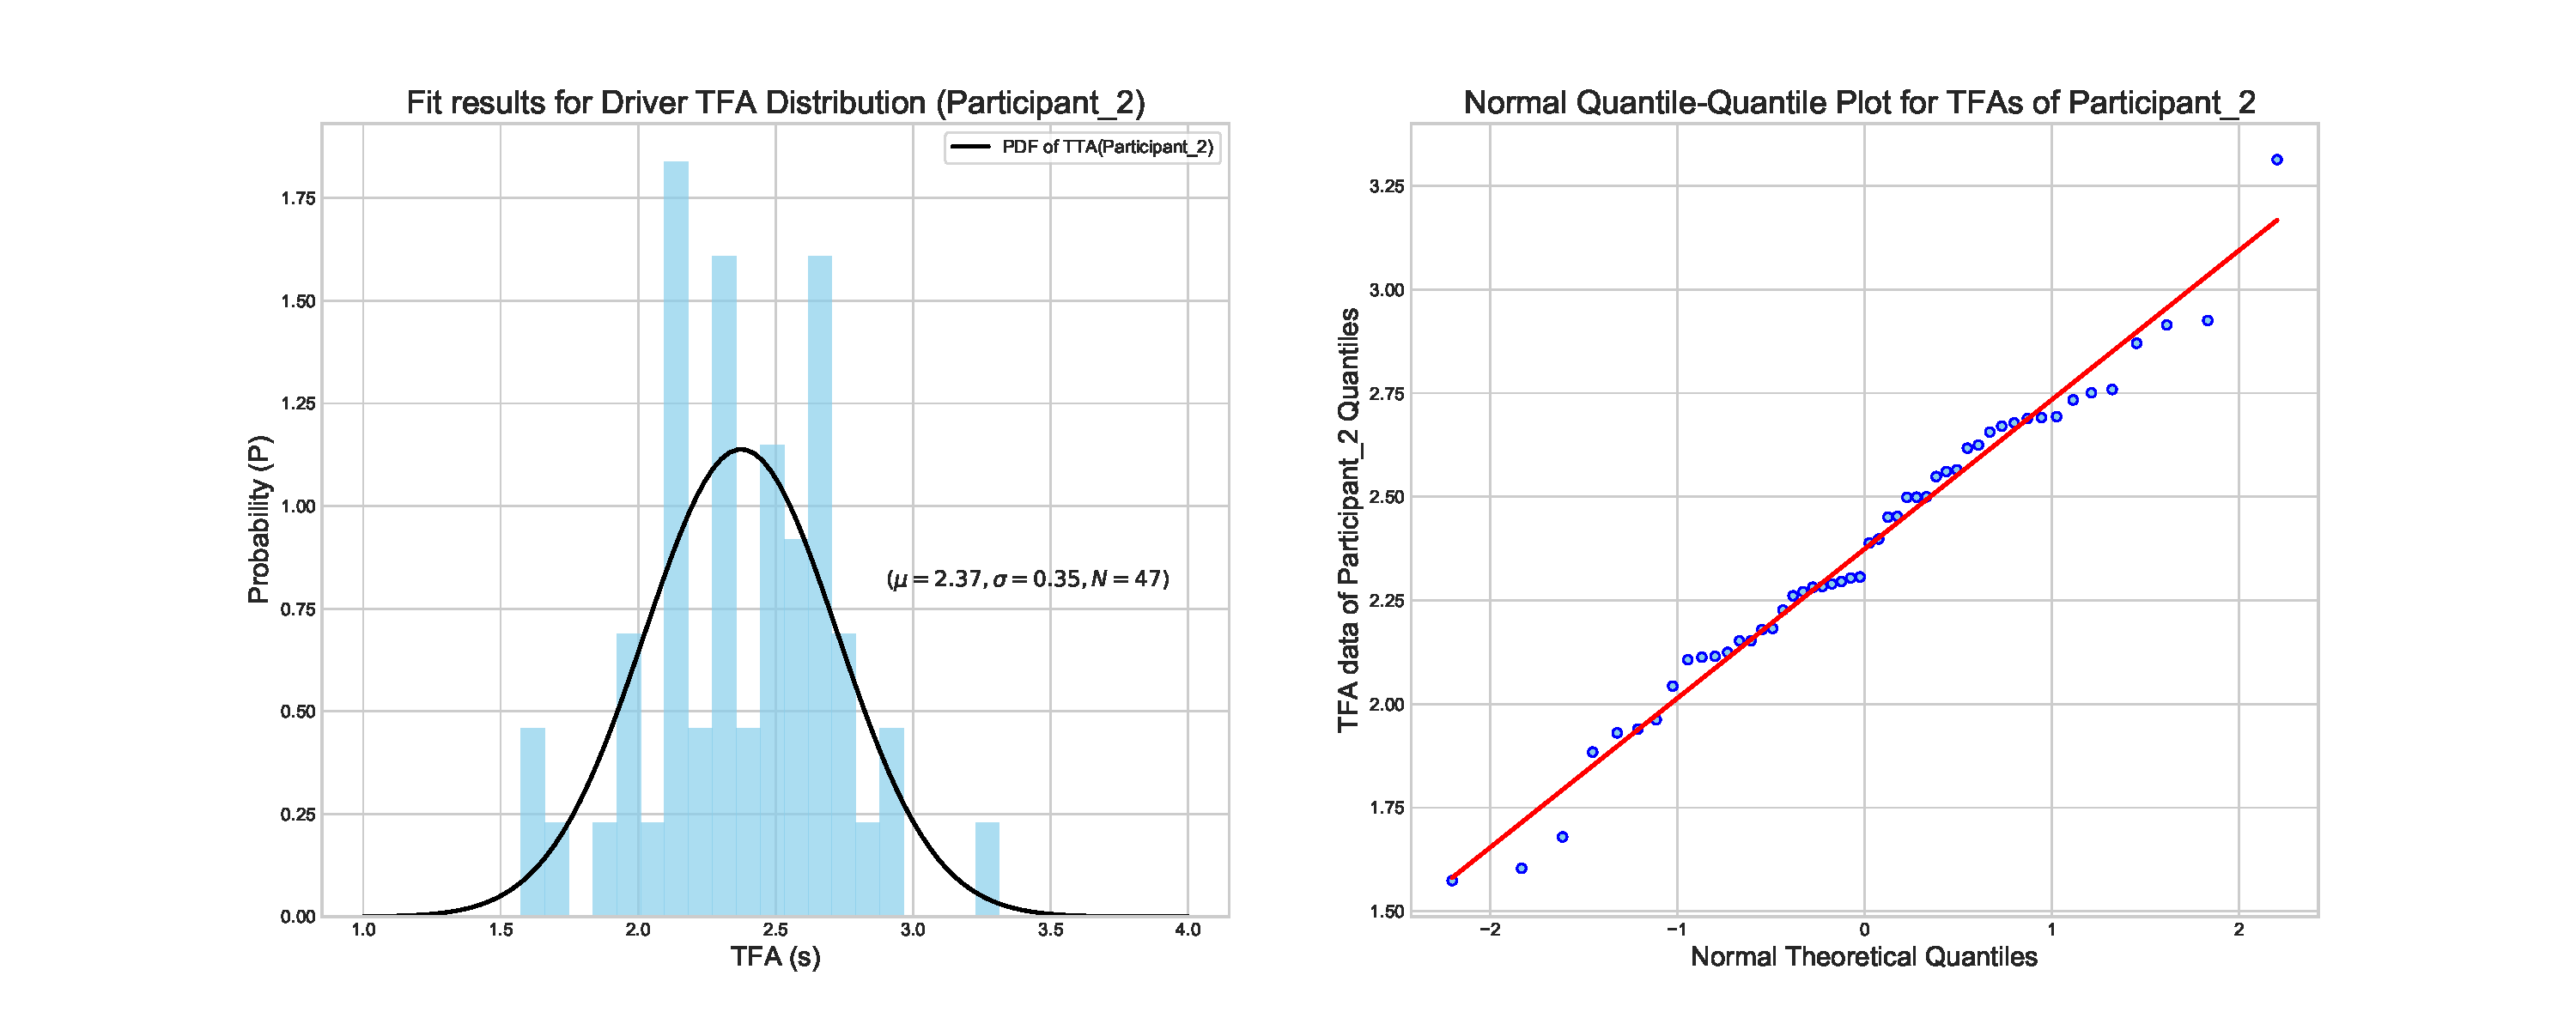
\includegraphics[width=0.8\paperwidth]{Participant_2_0_fitting.pdf}}
\end{center}
\caption{TFA results of participant 2 displayed in histogram. The solid curve is the TFA distribution of participant 2 approximated by Normal distribution ($\mu = 2.37, \sigma = 0.35, N = 47$). Speed of the vehicle while braking was set to 5 m/s.}
\label{fig:TFA_distr_2} 
\end{figure}

\begin{figure}[htbp!]
\begin{center}
\makebox[0pt]{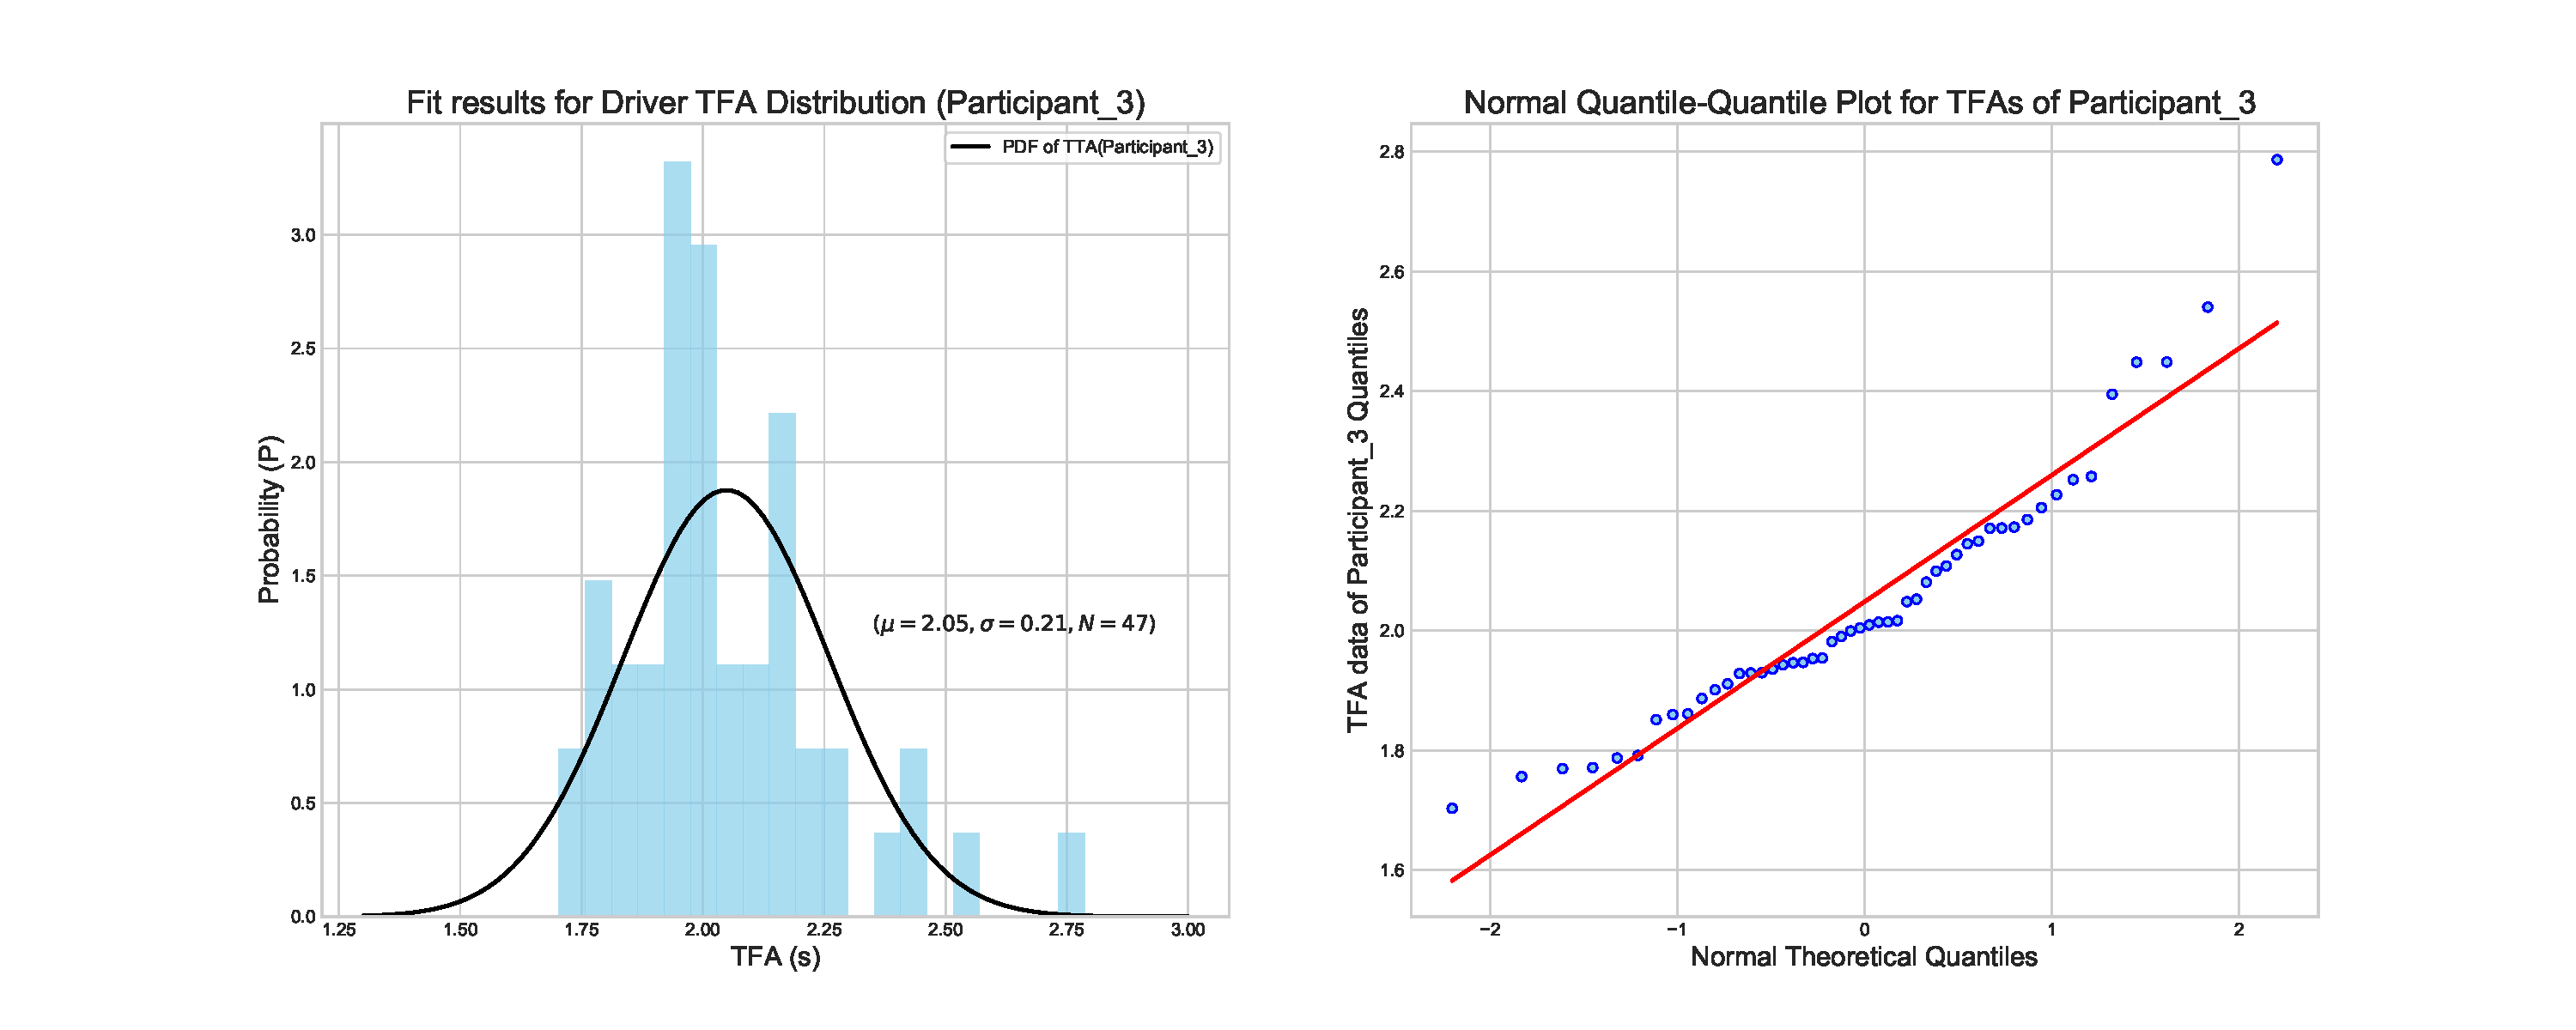
\includegraphics[width=0.8\paperwidth]{Participant_3_0_fitting.pdf}}
\end{center}
\caption{TFA results of participant 3 displayed in histogram. The solid curve is the TFA distribution of participant 3 approximated by Normal distribution ($\mu = 2.05, \sigma = 0.21, N = 47$). Speed of the vehicle while braking was set to 5 m/s.}
\label{fig:TFA_distr_3} 
\end{figure}

In Fig.~\ref{fig:TFA_distr_1}, Fig.~\ref{fig:TFA_distr_2} and Fig.~\ref{fig:TFA_distr_3}, sub-figures on the left are experimental TFA results plotted in histograms while sub-figures on the right are \ac{Q-Q Plots} using the same sets of TFA data. Q-Q plot is a graphical tool that can be used to examine the plausibility of the examined data coming from a theoretical distribution which is the Normal distribution in our case. One should note that Q-Q plots are merely a visual checking method that can give us an idea of how close the distribution of sampling data is comparing to theoretical one. Red solid lines in each figures are standard lines representing the theoretical results if the subject distribution is also a Normal distribution, in other words, closer the points to the red line higher chance the subject data is normally distributed.  

What we can learn from the figures is that TFA distribution of a single driver can be approximated by the Normal distribution if given large enough number of samples. To examine whether the TFA of general people is also normally distributed, all TFA data of participants are combined together in Fig.~\ref{fig:TFA_distr_combined}. Although the number of volunteers is not large enough, we can still learn from Fig.~\ref{fig:TFA_distr_combined} that combined distribution of drivers' TFA can also be approximated by Normal distribution. This result is actually unsurprising providing that all three individual TFA distributions are normally distributed.

\begin{figure}[htbp!]
\begin{center}
\makebox[0pt]{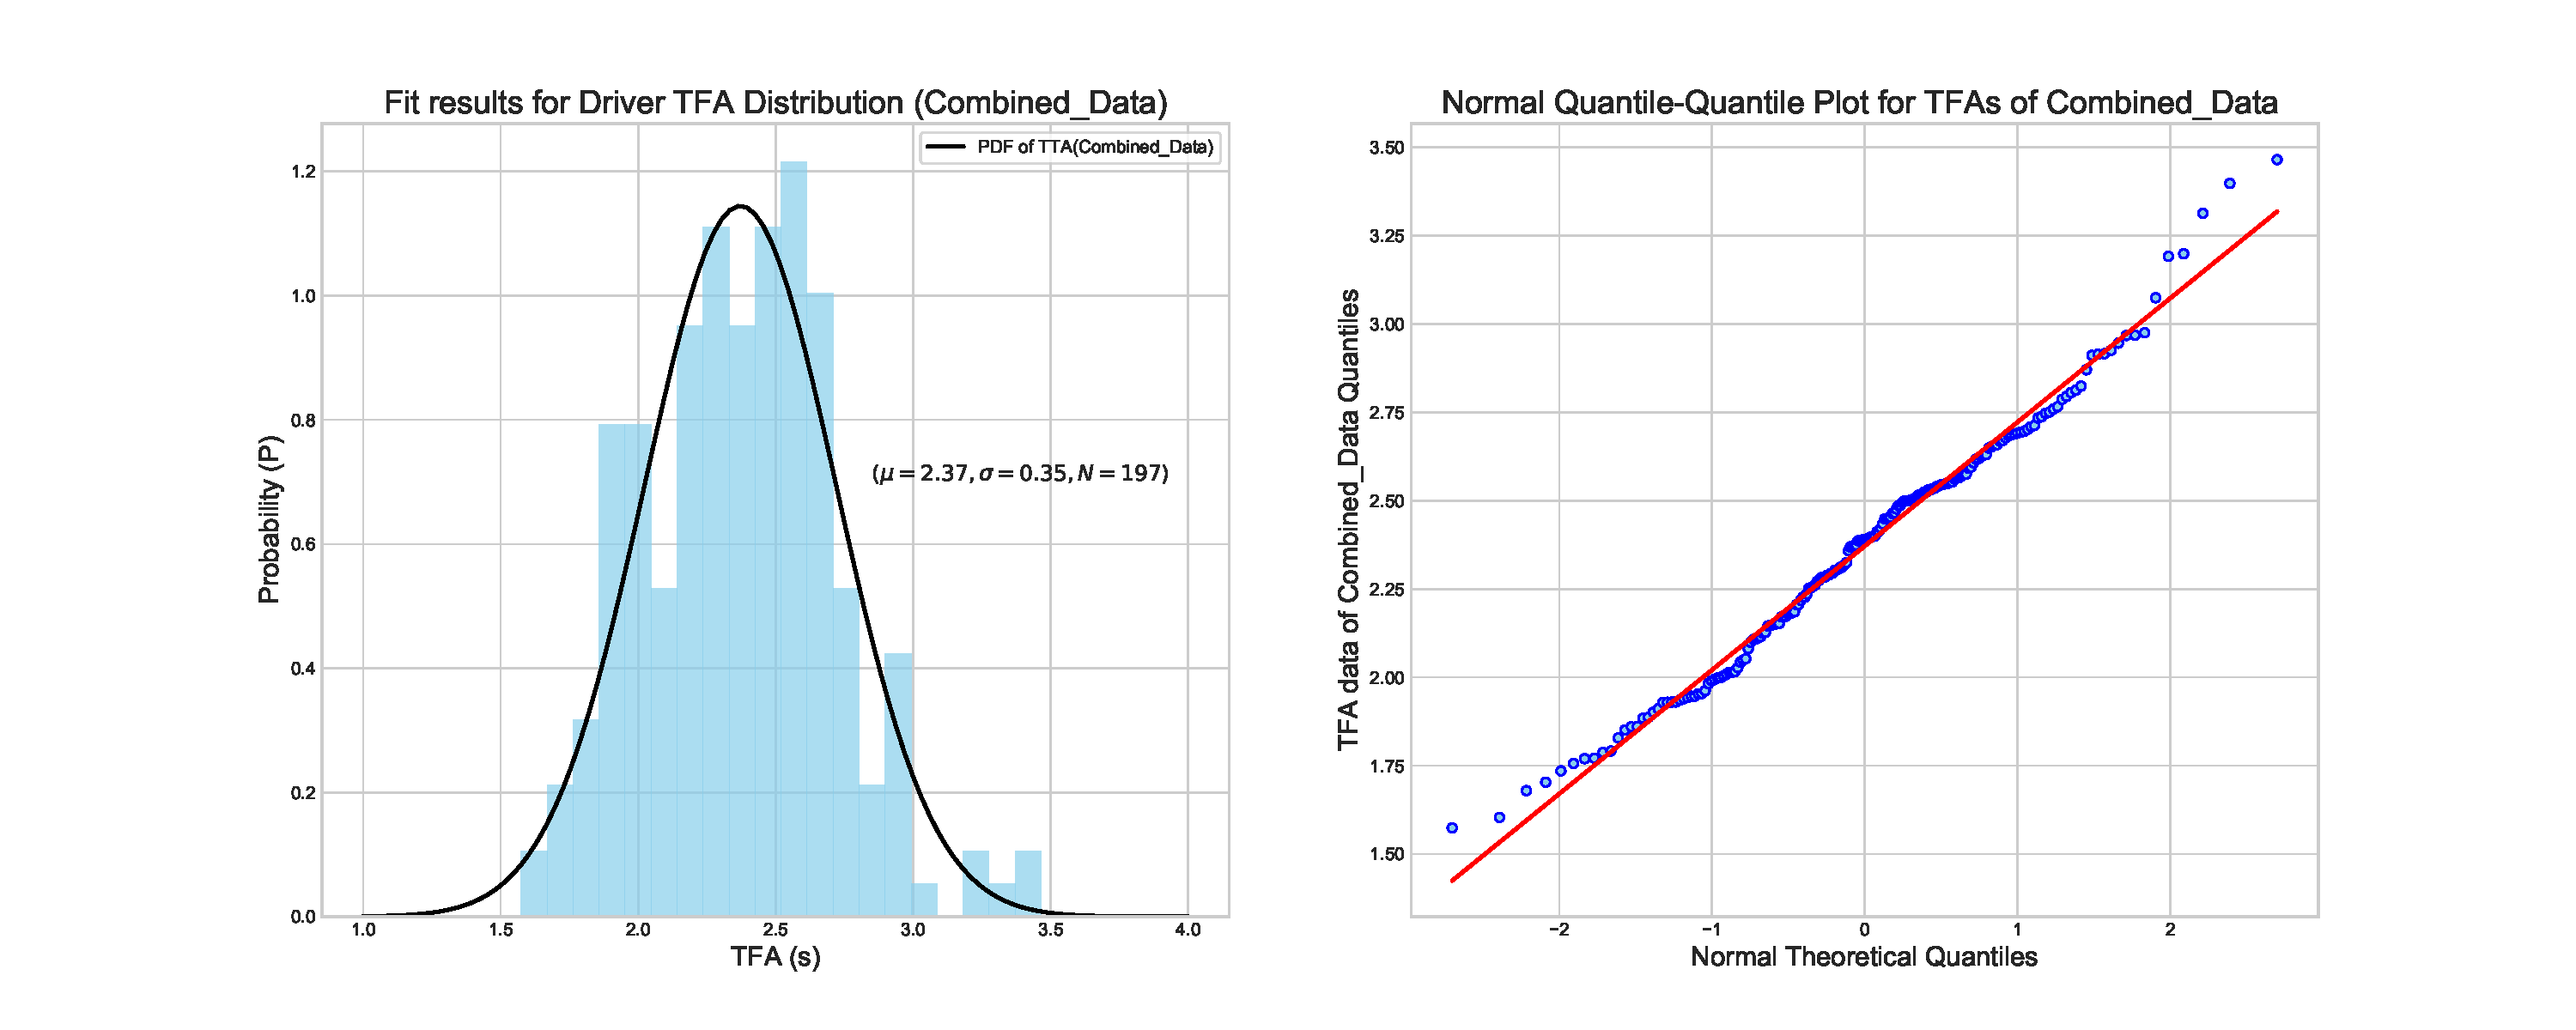
\includegraphics[width=0.75\paperwidth]{Combined_Data_0_fitting.pdf}}
\end{center}
\caption{TFA results of all participants are displayed in histogram. The solid curve is the TFA distribution of combined data of participants approximated by Normal distribution ($\mu = 2.37, \sigma = 0.35, N = 197$). Speed of the vehicle while braking was set to 5 m/s.}
\label{fig:TFA_distr_combined} 
\end{figure}

Knowing the TFA distribution for both individual and general people can be approximated by Normal distribution, the probability of a driver braking could be inferred effortlessly using the probability density function of the Normal distribution.

 
%%%%%%%%------------------------------%%%%%%%%%
%%%%%%%%-----------SUBSECTION---------%%%%%%%%%
%%%%%%%%------------------------------%%%%%%%%%
\subsection{TFA Probability Density Function}
\label{sub:TFA PDF}

From the previous section, the distribution of TFA is identified. In order to describe the human decision making process in a probabilistic way, the probability density function (PDF) of the TFA distribution is used. PDF is a function that defines the continuous random variables. A point on the PDF represents the \textit{likelihood} that the value of the random variable equals the sample value. Hence, an area under the curve of PDF would stand for the \textit{probability} of the random variable falling within that range. 

We can turn the grey area in Fig.~\ref{fig:TTC_TFA} into a PDF as in Fig.~\ref{fig:TTC_distribution}. In this case, when a certain value of TTC within the PDF of TFA of general people is reached, the area under the PDF and right to this value represents the probability of the brake being applied. To make it clearer, let us assume the TTC of a vehicle driving towards a crossroad now is 3. At this instance, the probability for the driver to brake would then be the area under the PDF and right to the value 3, which is 50\% since 3 is also the mean value of the TFA distribution in Fig.~\ref{fig:TTC_distribution}. Drivers with TFA greater than 3 would have braked before the TTC reached 3 because the TTC drops as the host vehicle is driven toward the crossroad and the displacement to the node is decreasing according to Eqn.~\ref{eq:TTC_crossroad}. The concept behind using the area under the PDF and right to the current TTC as the probability to brake combines elements introduced in the previous sections, including using TTC as to indicate the time for braking (i.e. TFA) and approximating the TFA distribution with Normal distribution.

What should be noted here is that since whether the driver brakes or not, the displacement to the node during that time is always decreasing. According to Eqn.~\ref{eq:TTC_crossroad}, if the constant car speed is maintained, the value of TTC will fall down as the vehicle is driven toward the node. On the other hand, if the brake is applied, the TTC rises parabolically as shown in Fig.~\ref{fig:TTC_history}. Hence, before the brake is applied, the TTC used to calculate the probability is the TTC at the moment. The TTC used to calculate the probability after the brake is applied should then be the lowest TTC that occurs on the TTC curve of the host agent since the intention to brake during the braking process remains the same as the beginning of the action. We will use Fig.~\ref{fig:TTC_TFA_indicator} and ~\ref{fig:TTC_distribution} to further explain this idea. 

In Fig.~\ref{fig:TTC_TFA_indicator}, the dashed lines indicated by colored shapes (including squares, triangles and circles) on both sides represent the sampled moments during the braking process. Red squares indicating the TTC at 3 seconds on the time line, blue triangles at around 5.5 seconds and magenta circles at around 7 seconds. The corresponding moments are also labeled on the TFA distribution in Fig.~\ref{fig:TTC_distribution}. At 3 seconds (red squared connected with dashed line, using red line in short) the TTC of the host agent is around 4.2 seconds. We can then estimate from the PDF in Fig.~\ref{fig:TTC_distribution} that the probability of the vehicle stopping is 0.0013, which is the area right side of the red line. This result is reasonable since the TTC at this moment is still far from the TFA average which is 3. Similarly, when the time is at 5.6 seconds (blue line) the TTC at the time is around 3.1, so the probability of the vehicle stops rise to 0.401. As it comes to the time at 7 seconds (magenta line) the TTC becomes larger due to the brake, but as mentioned before, the rising of TTC indicates the agent is slowing down, which does not lower the probability to brake. So the probability of the host agent braking is still calculated using the lowest TTC value on the TTC curve which is 3.1, so the probability to brake is still 0.401.

\begin{figure}[htbp!]
\begin{center}
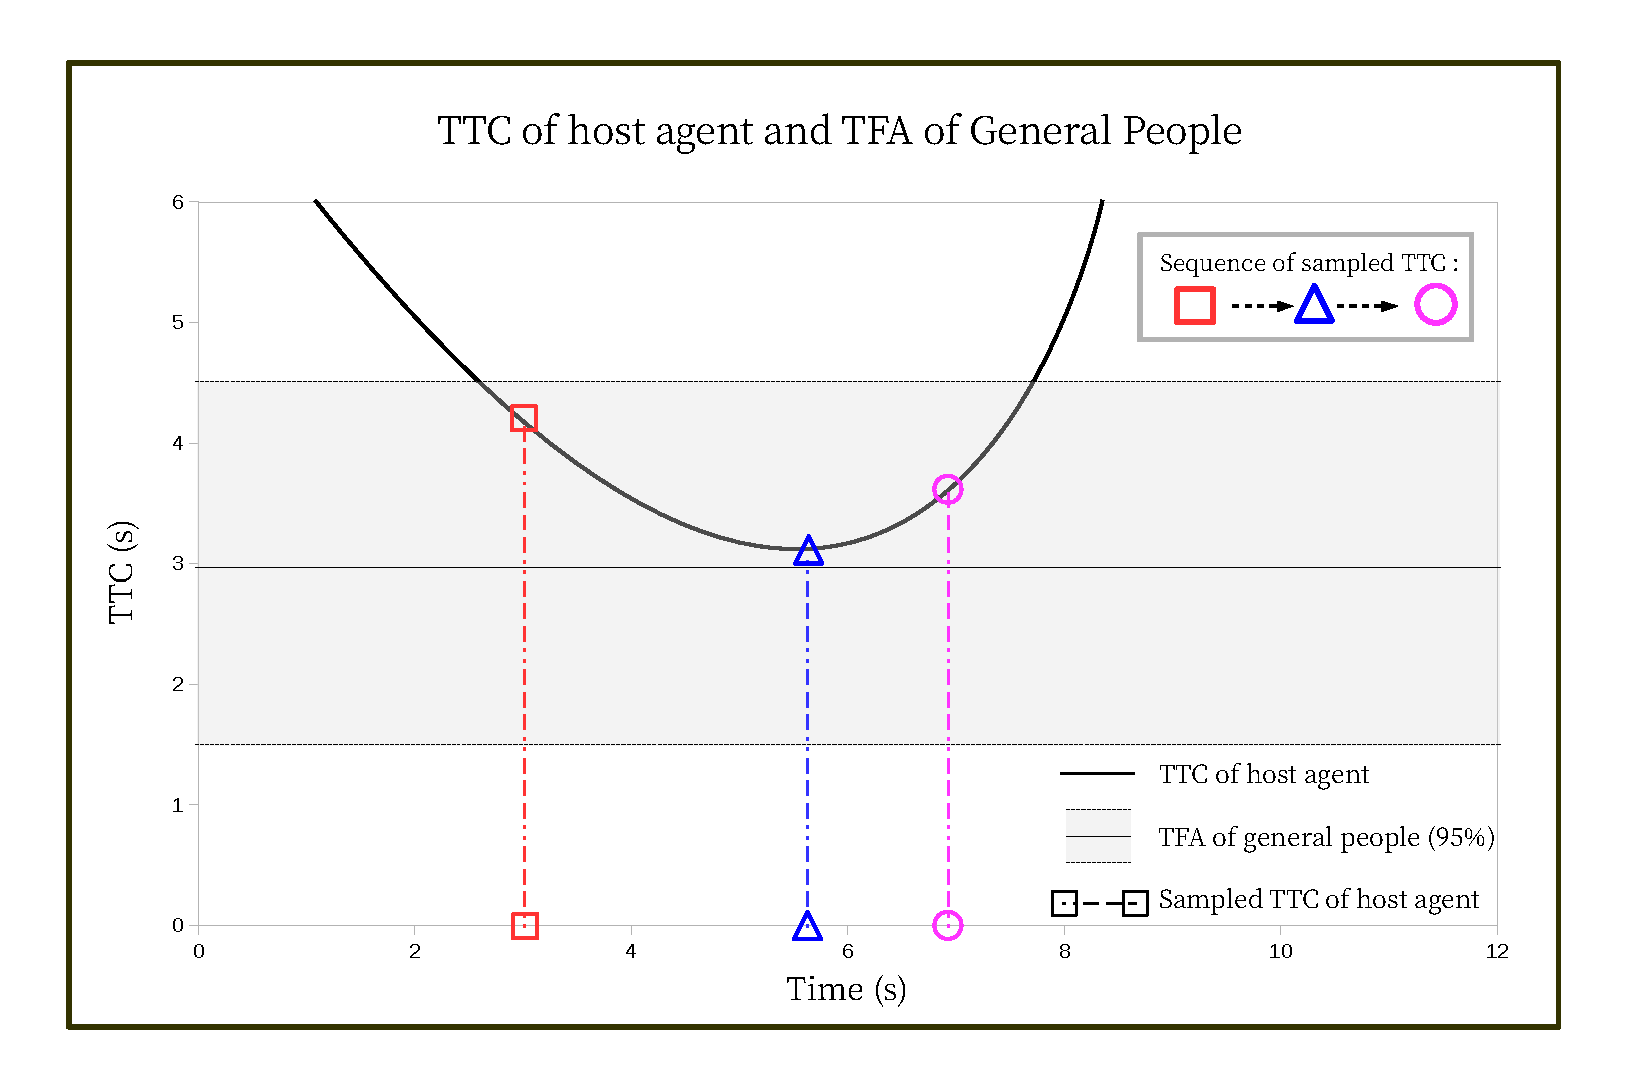
\includegraphics[scale=0.5]{TTC_probability_indicator.pdf}
\end{center}
\caption{Example of TFA of general people and TTC of the host agent.}
\label{fig:TTC_TFA_indicator} 
\end{figure}

\begin{figure}[htbp!]
\begin{center}
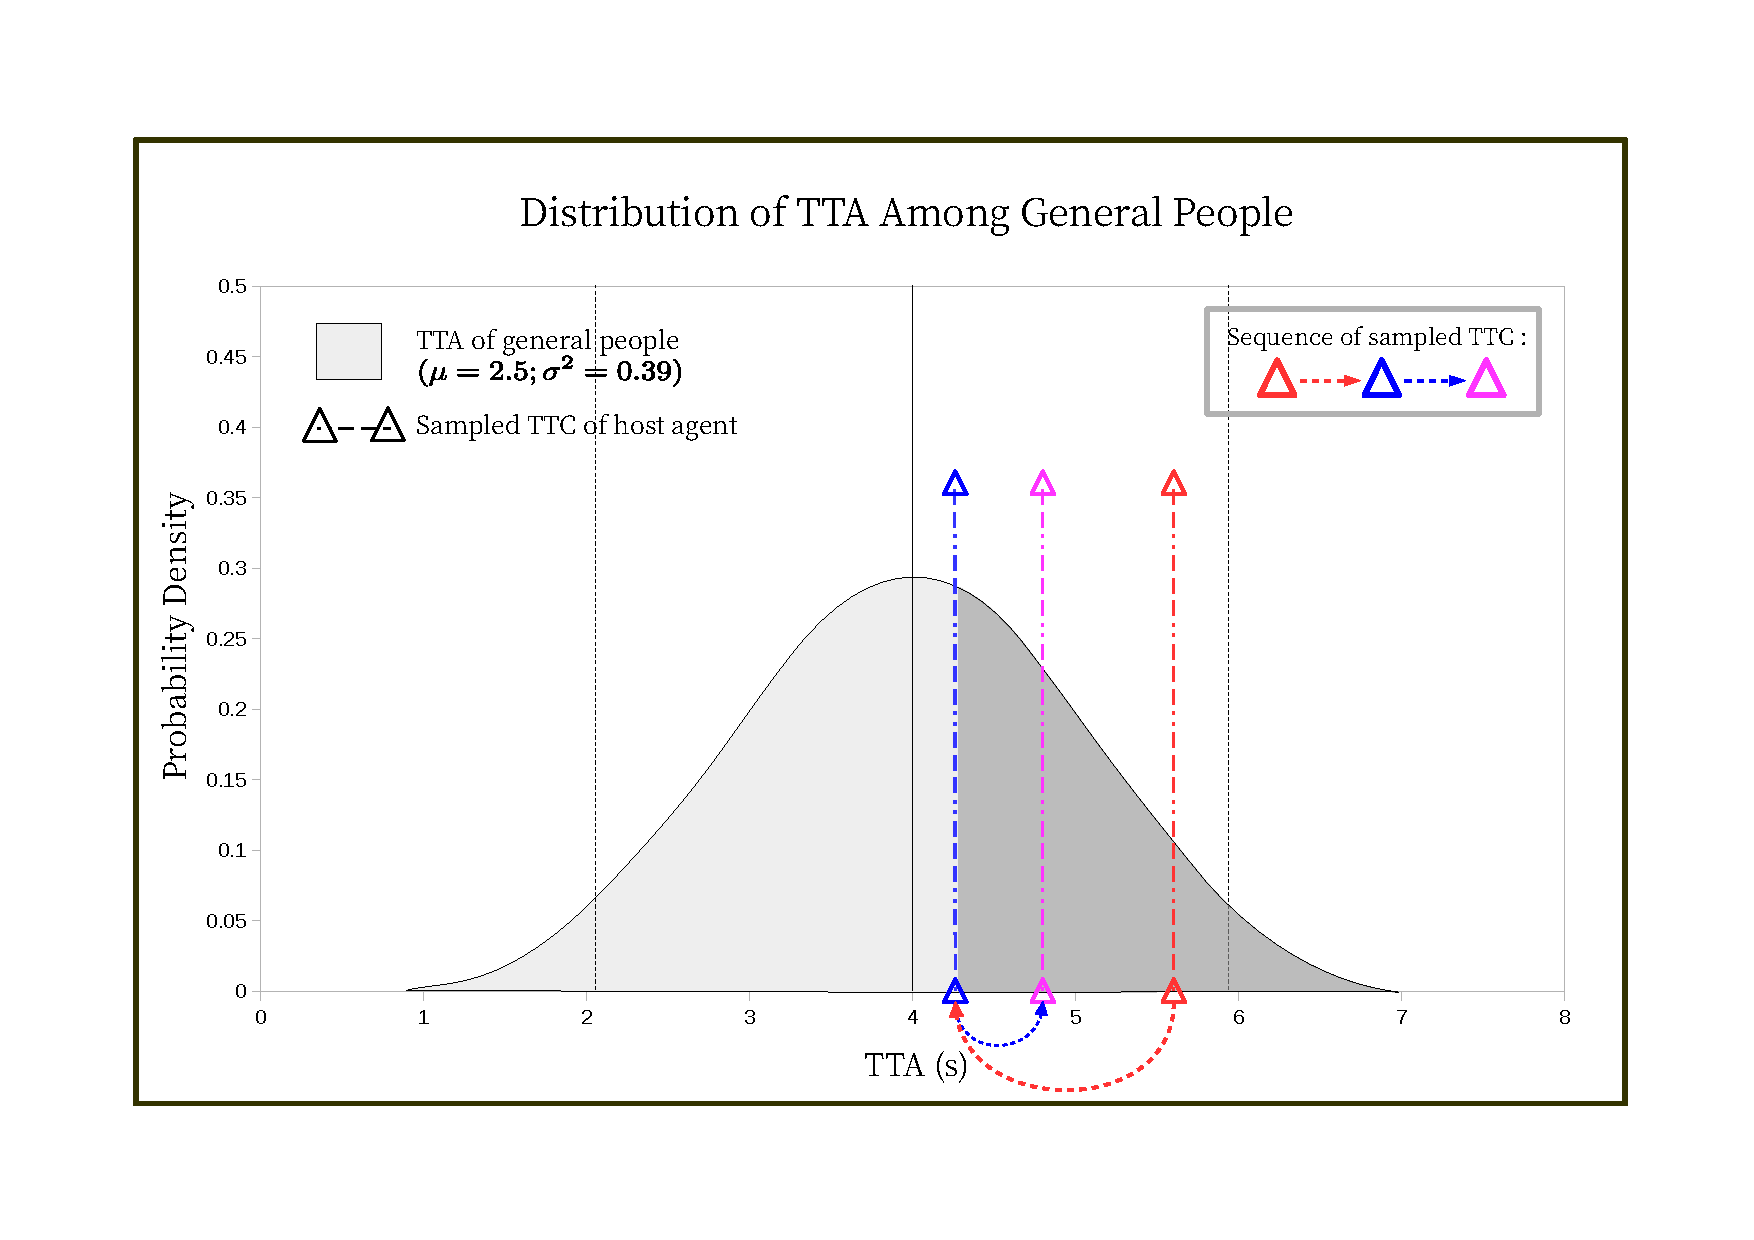
\includegraphics[scale=0.5]{TTC_probability_distribution.pdf}
\end{center}
\caption{Example of TFA distribution of general people.}
\label{fig:TTC_distribution} 
\end{figure}

So far we learned that the probability for the driver to brake is the integral of the PDF from the current, or the lowest in case the brake is applied, to the +inf. The probability to brake mentioned in the above paragraph refers to the intention that the driver brake to avoid potential obstacles. In the next section, the probability estimation method illustrated in this section will be used to evaluate the probability for the driver to yield to other traffic participants at the crossroad described in section \ref{sub:crossroad}.


%%%%%%%%%%%%%%%%%%%%%%%%%%%%%%%%%%%%%%%%%%%%%%%%%%%%%%%%%%%%%%%%%%%%%%%%
%%%%%%%%%%               SECTION SECTION SECTION               %%%%%%%%%
%%%%%%%%%%%%%%%%%%%%%%%%%%%%%%%%%%%%%%%%%%%%%%%%%%%%%%%%%%%%%%%%%%%%%%%%
\section{ Probability of Yielding}
\label{sec:POY}

To this moment, the probability for a driver to brake can be calculated using the PDF of TFA of general people, but merely integrating the PDF is still inadequate to explain the probability for the driver to yield. For example, assuming a driver drives towards the node without decelerating. Throughout the whole operation, the TTC of the host agent decreases, resulting the rising of the \ac{POY} (increasing area right to the current TTC and under the TFA distribution), which is a contradiction to our goal. Additionally, the TFA distribution for a driver is a function of the speed, hence the distribution Fig.~\ref{fig:TFA_distr_combined} represents the TFA distribution of general people (combined data of participants). In preparation for the driver yielding model at crossroads, firstly the TFA distribution model that can account for the distributions under different  speed is required, secondly parameters that are able to explain all possible circumstances should be included.   


%%%%%%%%------------------------------%%%%%%%%%
%%%%%%%%-----------SUBSECTION---------%%%%%%%%%
%%%%%%%%------------------------------%%%%%%%%%
\subsection{TFA Distribution Modeling}

In this work, we focus on the crossroad scenario described earlier where two drivers drive toward the node (the intersection of their courses) on the paths perpendicularly to each other at the same time. The term $\mathbf{d_{node,i, t}}$ in Eqn.~(\ref{eq:TTC_crossroad}) denotes the displacements to the node that change along with time. In other words, at the moment that the driver has the intention to yield, this term will then represent the distance required for the vehicle braking and keeping a distance between the vehicle and the node when fully stopped which is the \textit{distance left before action} in Fig.~\ref{fig:TFA_model} .

\begin{figure}[htbp!]
\begin{center}
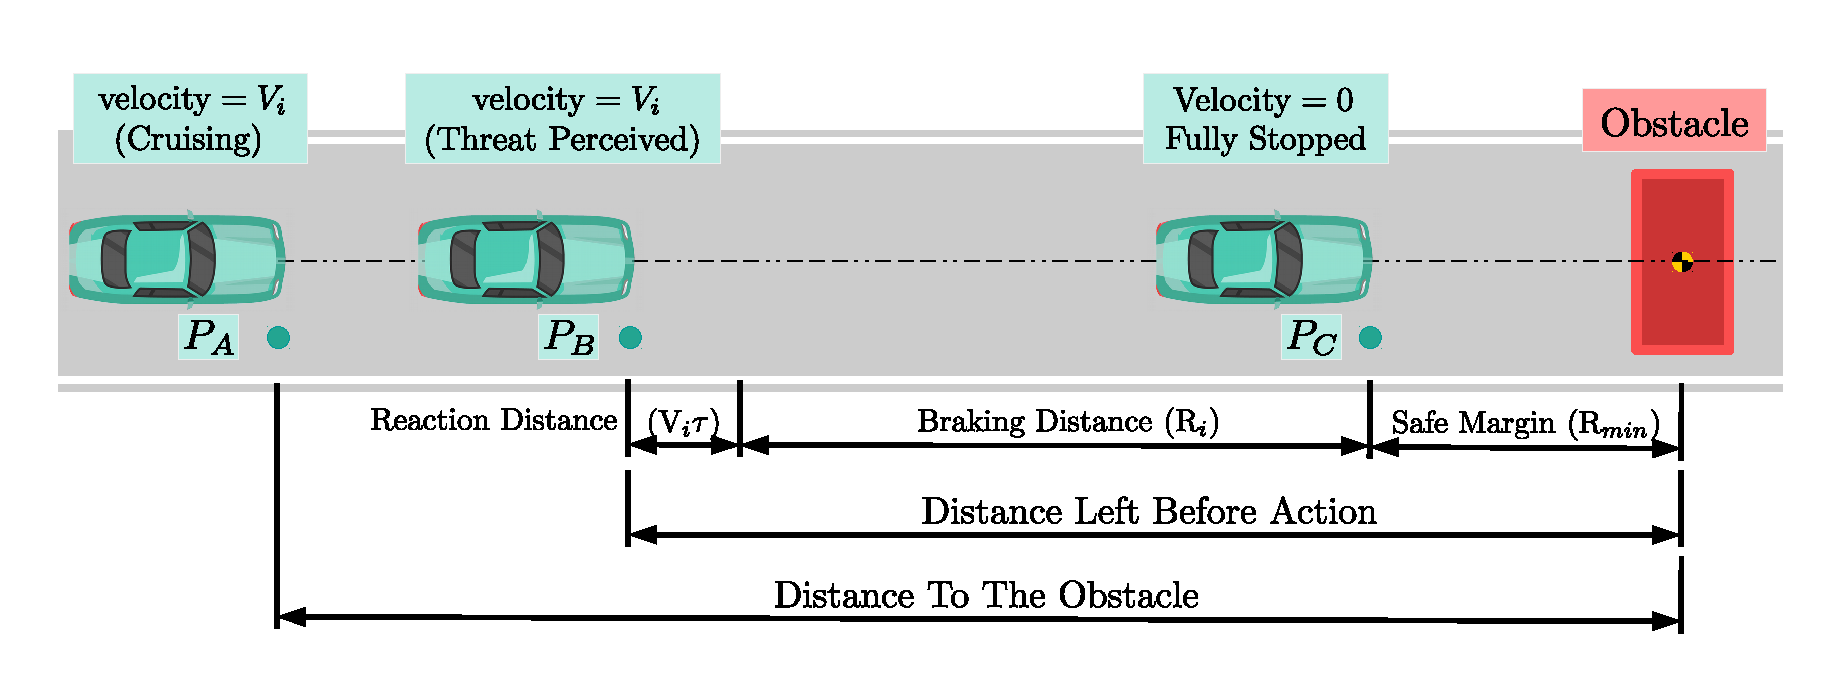
\includegraphics[scale=0.45]{TFA_TTC_model.pdf}
\end{center}
\caption{Decomposing the distance left before action (apply the brake).}
\label{fig:TFA_model} 
\end{figure}


The distance left before action is broken down into three parameters in Fig.~\ref{fig:TFA_model}, which are reaction time, braking distance and the safe margin (i.e. the distance left when fully stopped). The reaction time is the combination of the human perception-reaction delay and the vehicle actuation delay, i.e., these are the time that drivers need from seeing a potential threat to hitting the brake and the time the brake system need to decelerate the vehicle after the applying the brake. The braking distance stands for the distance the vehicle need to be fully stopped. And the safe margin is the distance left between the host vehicle and the obstacle when the vehicle is fully stopped. The reaction time can be expressed as 

\begin{equation}
\text{Reaction Time} = {v_i}\tau
\label{eq:V_tau}
\end{equation}

\noindent where ${v_i}$ is the speed of the subject vehicle at the very moment when the brake is applied and $\tau$ is the combination of system and driver delays as mentioned earlier. The second parameter is the braking distance, denoting as

\begin{equation}
R_{i} = \frac{v_i^2}{2a_{dec}}
\label{eq:R_i}
\end{equation}

where ${v_i}$ is same as the one in Eqn.~\ref{eq:V_tau} which stands for the speed of the vehicle at that moment while $a_{dec}$ represents the average deceleration applied during the braking. What should be noted here is that Eqn.~\ref{eq:R_i} is based on the assumption that the constant deceleration is applied throughout the entire braking process. The last parameter, safe margin, is denoted as $R_{min}$ which stands for the safe distance that the driver left after the vehicle is fully stopped. For the sake of making data extraction easier, the $R_{min}$ is defined as distance from the center of one vehicle to another. Combining these three parameters we have the distance left for braking as

\begin{equation}
\text{Distance Left Before Braking} = R_i+v_i\tau+R_{min}
\label{eq:TFA_distance}
\end{equation}

One should have been aware of the fact that the meaning of this distance is exactly the distance term in Eqn.~\ref{eq:TTC_crossroad} when the TTC at this moment equals the TFA of the driver, since Eqn.~\ref{eq:TFA_distance} is the estimated distance needed for the driver if he or she attempts to yield at this moment.  So dividing Eqn.~\ref{eq:TFA_distance} by the speed of the subject vehicle ${v_i}$ we will have

\begin{equation}
\text{TFA}_{est} = \frac{R_i+v_i\tau+R_{min}}{v_i} 
\label{eq:TFA_est}
\end{equation}


\noindent where ${TFA}_{est}$ represents the estimated TFA of the driver. This ${TFA}_{est}$ is then applied as the mean value of the TFA distribution under the vehicle speed ${v_i}$. Combining all the element, the TFA distribution is now described as


\begin{equation}
\text{TFA} \sim \mathcal{N}(\text{TFA}_{est},\,\sigma_{est}^{2})\,.
\label{eq:TFA_distribution}
\end{equation}

and the value of the variance $\sigma^2$ is defined as 

\begin{equation}
\sigma_{est} = \gamma \cdot \text{TFA}_{est}
\label{eq:TFA_distribution}
\end{equation}

\noindent where $\gamma$ is the coefficient for standard deviation, which is obtained from the ratio of $\mu$ and $\sigma$ obtained from the approximated normal distribution of TFA. 

As mentioned in Section \ref{sub:TFA Distribution}, the TFA distribution is suggested to vary under different velocity. It seems more plausible using the TFA distribution described in Eqn.~\ref{eq:TFA_est}. To confirm this idea, the experiments similar to the one conducted in Section \ref{sub:TFA Distribution}( to prove the TFA distribution is normally distributed ) is repeated but under different velocity at the moment of the brake. The velocity varies from 2.5 to 5 m/s using 0.5 as the step. Results of two participants are shown in Fig~.\ref{fig:Par1TFADifSpeed} and Fig~.\ref{fig:Par3TFADifSpeed}.

\begin{figure}[htbp!]
\begin{center}
\makebox[0pt]{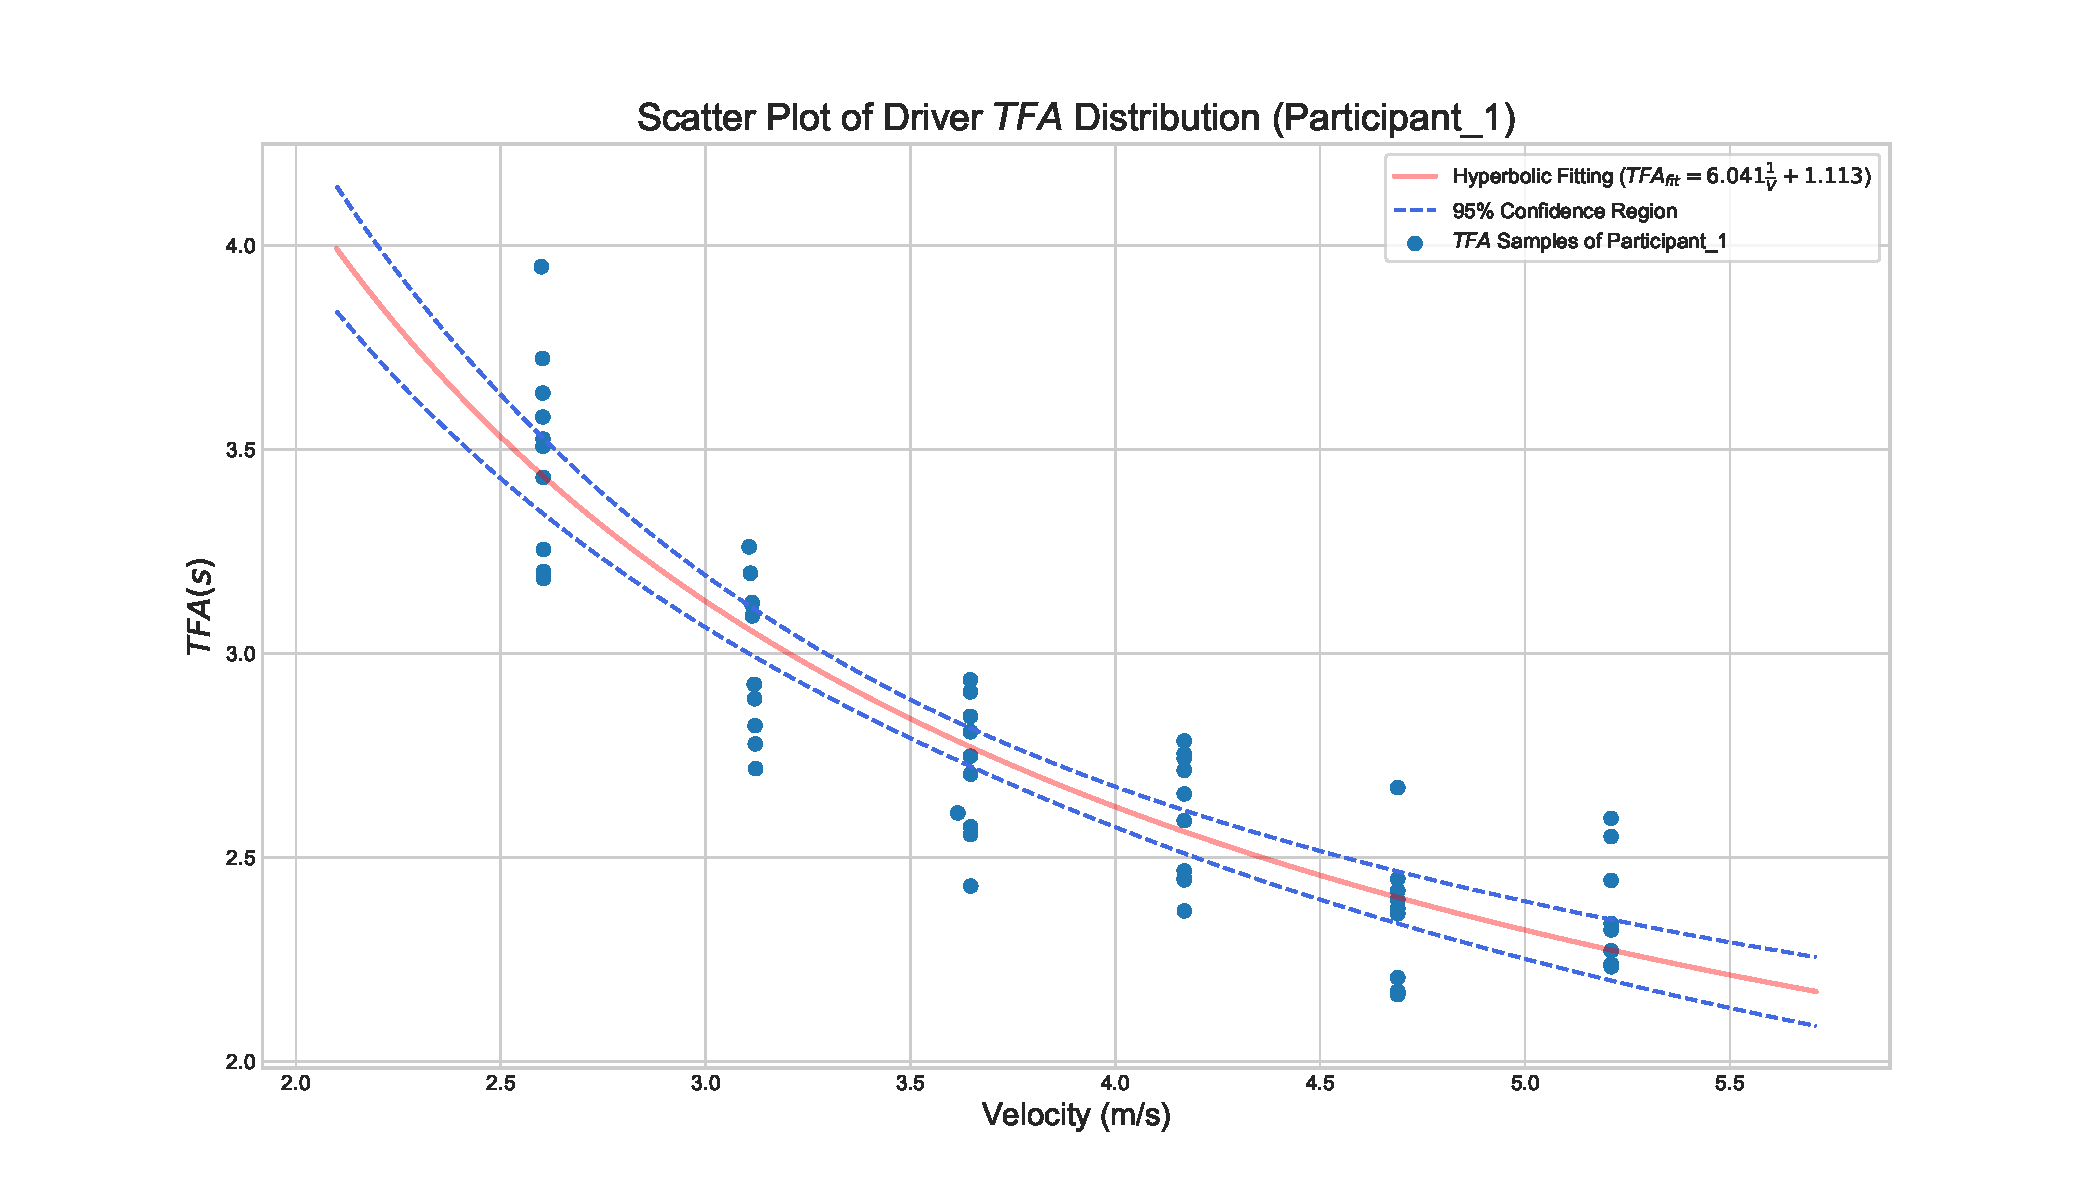
\includegraphics[width=0.7\paperwidth]{/Participant_1_TFA_polyfit.pdf}}
\end{center}
\caption{The TFA scatter plot of Participant 1 under various velocities.}
\label{fig:Par1TFADifSpeed} 
\end{figure}

\begin{figure}[htbp!]
\begin{center}
\makebox[0pt]{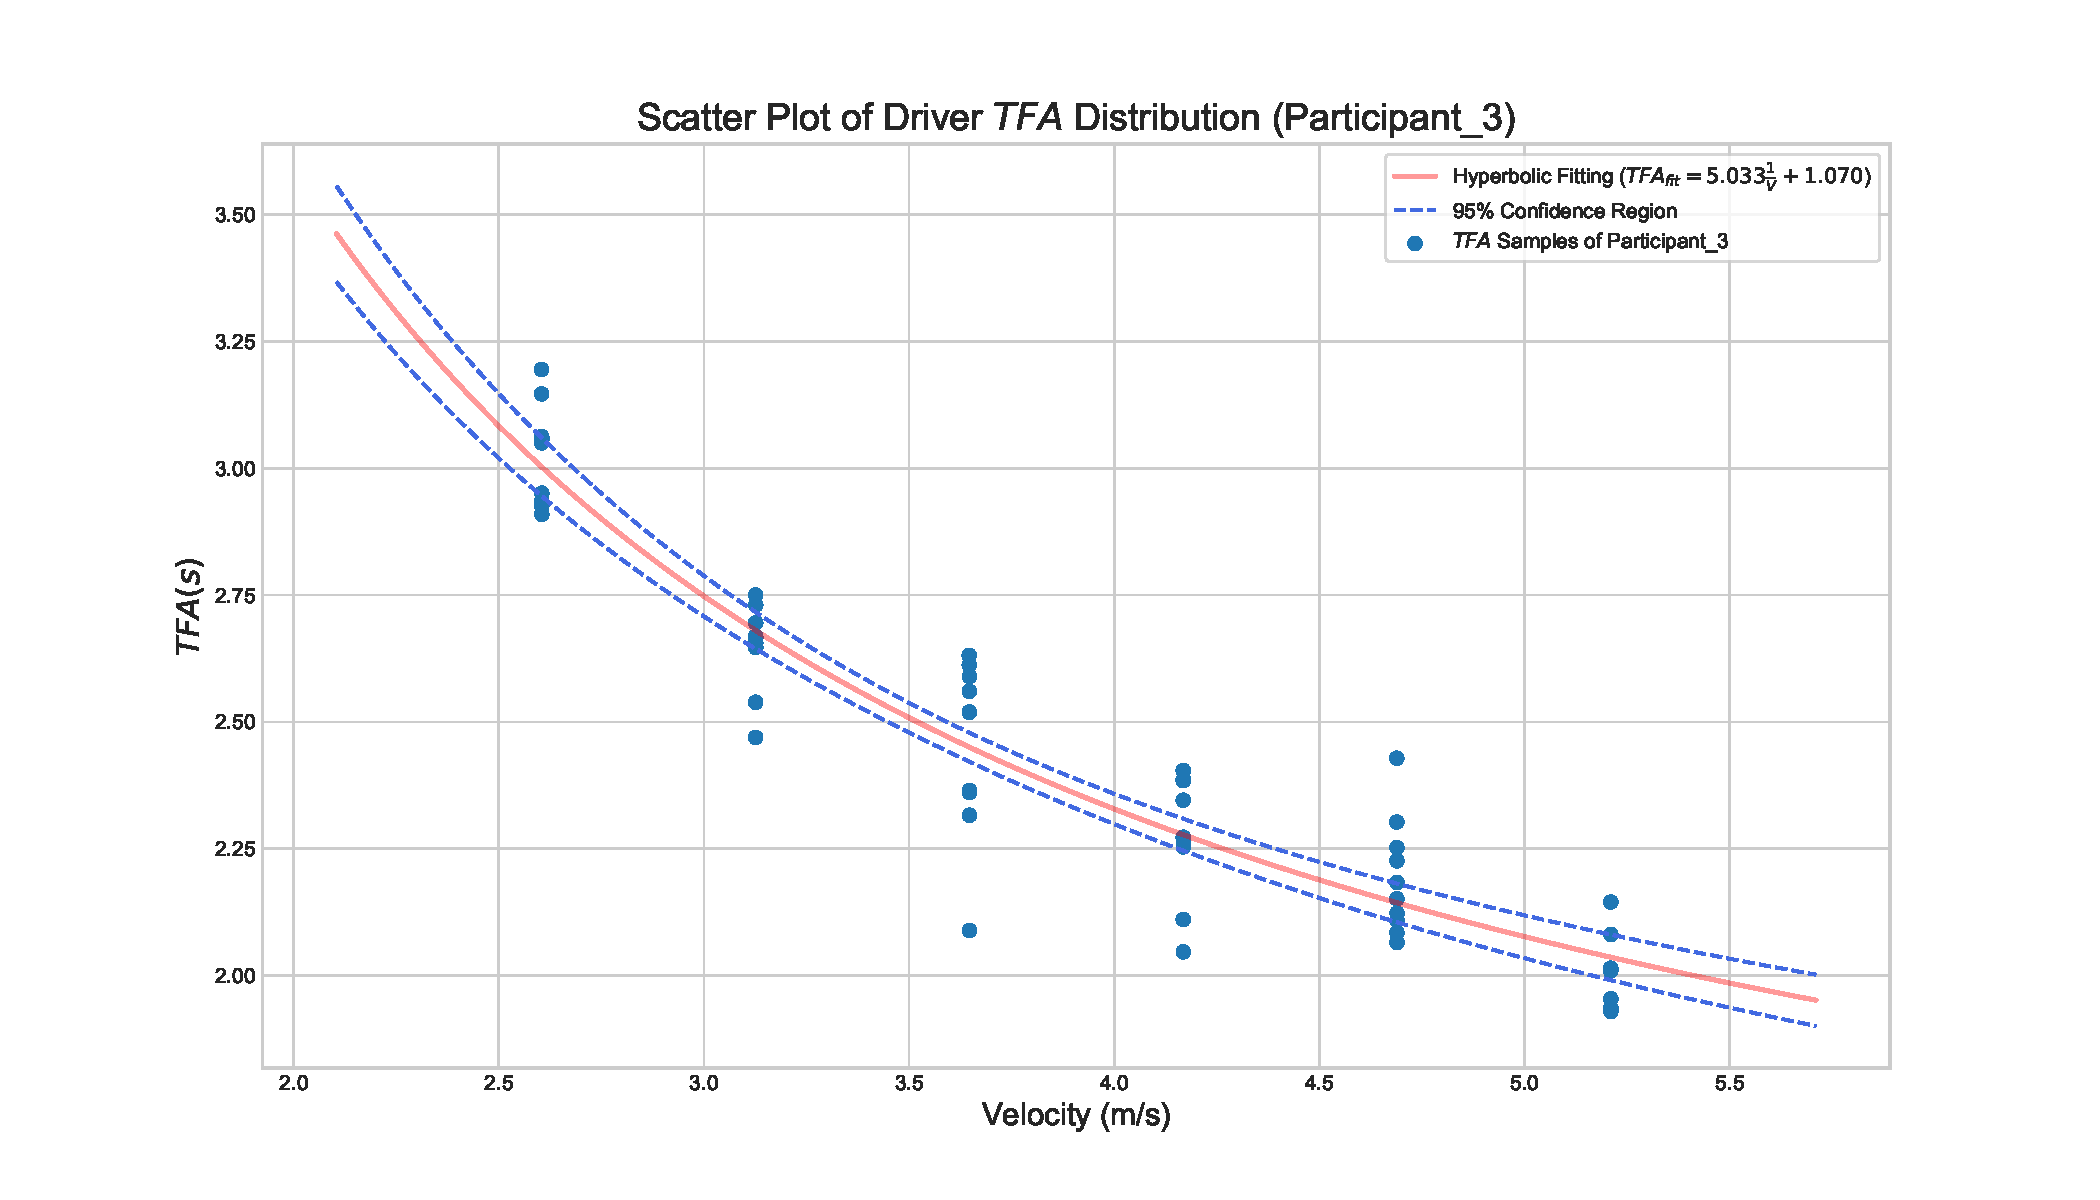
\includegraphics[width=0.7\paperwidth]{/Participant_3_TFA_polyfit.pdf}}
\end{center}
\caption{The TFA scatter plot of Participant 3 under various velocities.}
\label{fig:Par3TFADifSpeed} 
\end{figure}

In Fig~.\ref{fig:Par1TFADifSpeed} and Fig~.\ref{fig:Par3TFADifSpeed}, the blue dots are the collected data while the red line represents the curve fitting using hyperbolic equation. The reason for choosing hyperbolic equation is to provide evidence of how accurate the proposed $TFA_{est}$ equation is. It turns out that the TFA varies under different velocity following the hyperbolic equation, which is similar to the relation in Eqn.~\ref{eq:TFA_est}.

Now the ${TFA}_{est}$ is identified to be a function of ${v_i}$ as described in Eqn.~\ref{eq:TFA_est}, there are only three parameters left to be identified before completing the TFA distribution model. Since $\tau$ represents the reaction time of the driver which is biological trait, it can be considered as a constant under different speed. $R_{min}$ and $a_{dec}$ on the other hand, are functions of velocity due to different possible consequences at different velocities. For instance, people might have more aggressive actions when at lower speed (e.g. smaller $R_{min}$ for closer distance to the other vehicle after stopped) since everything is under control (i.e. the severity of the collision is low). While at high speed, however, drivers tend to act more conservatively (e.g. larger $R_{min}$ to keep a "safer margin") to avoid the serious collision. Experiments are conducted and shown to confirm the idea.

To estimate the parameters needed for TFA distribution of average drivers, data collected from participants are combined and analyzed in Fig.~\ref{fig:CombRMINDifSpeed} and Fig.~\ref{fig:CombADECDifSpeed}. The corresponding linear equation defining $R_{min}$ and $a_{dec}$ under various velocity are also presented.

\begin{figure}[htbp!]
\begin{center}
\makebox[0pt]{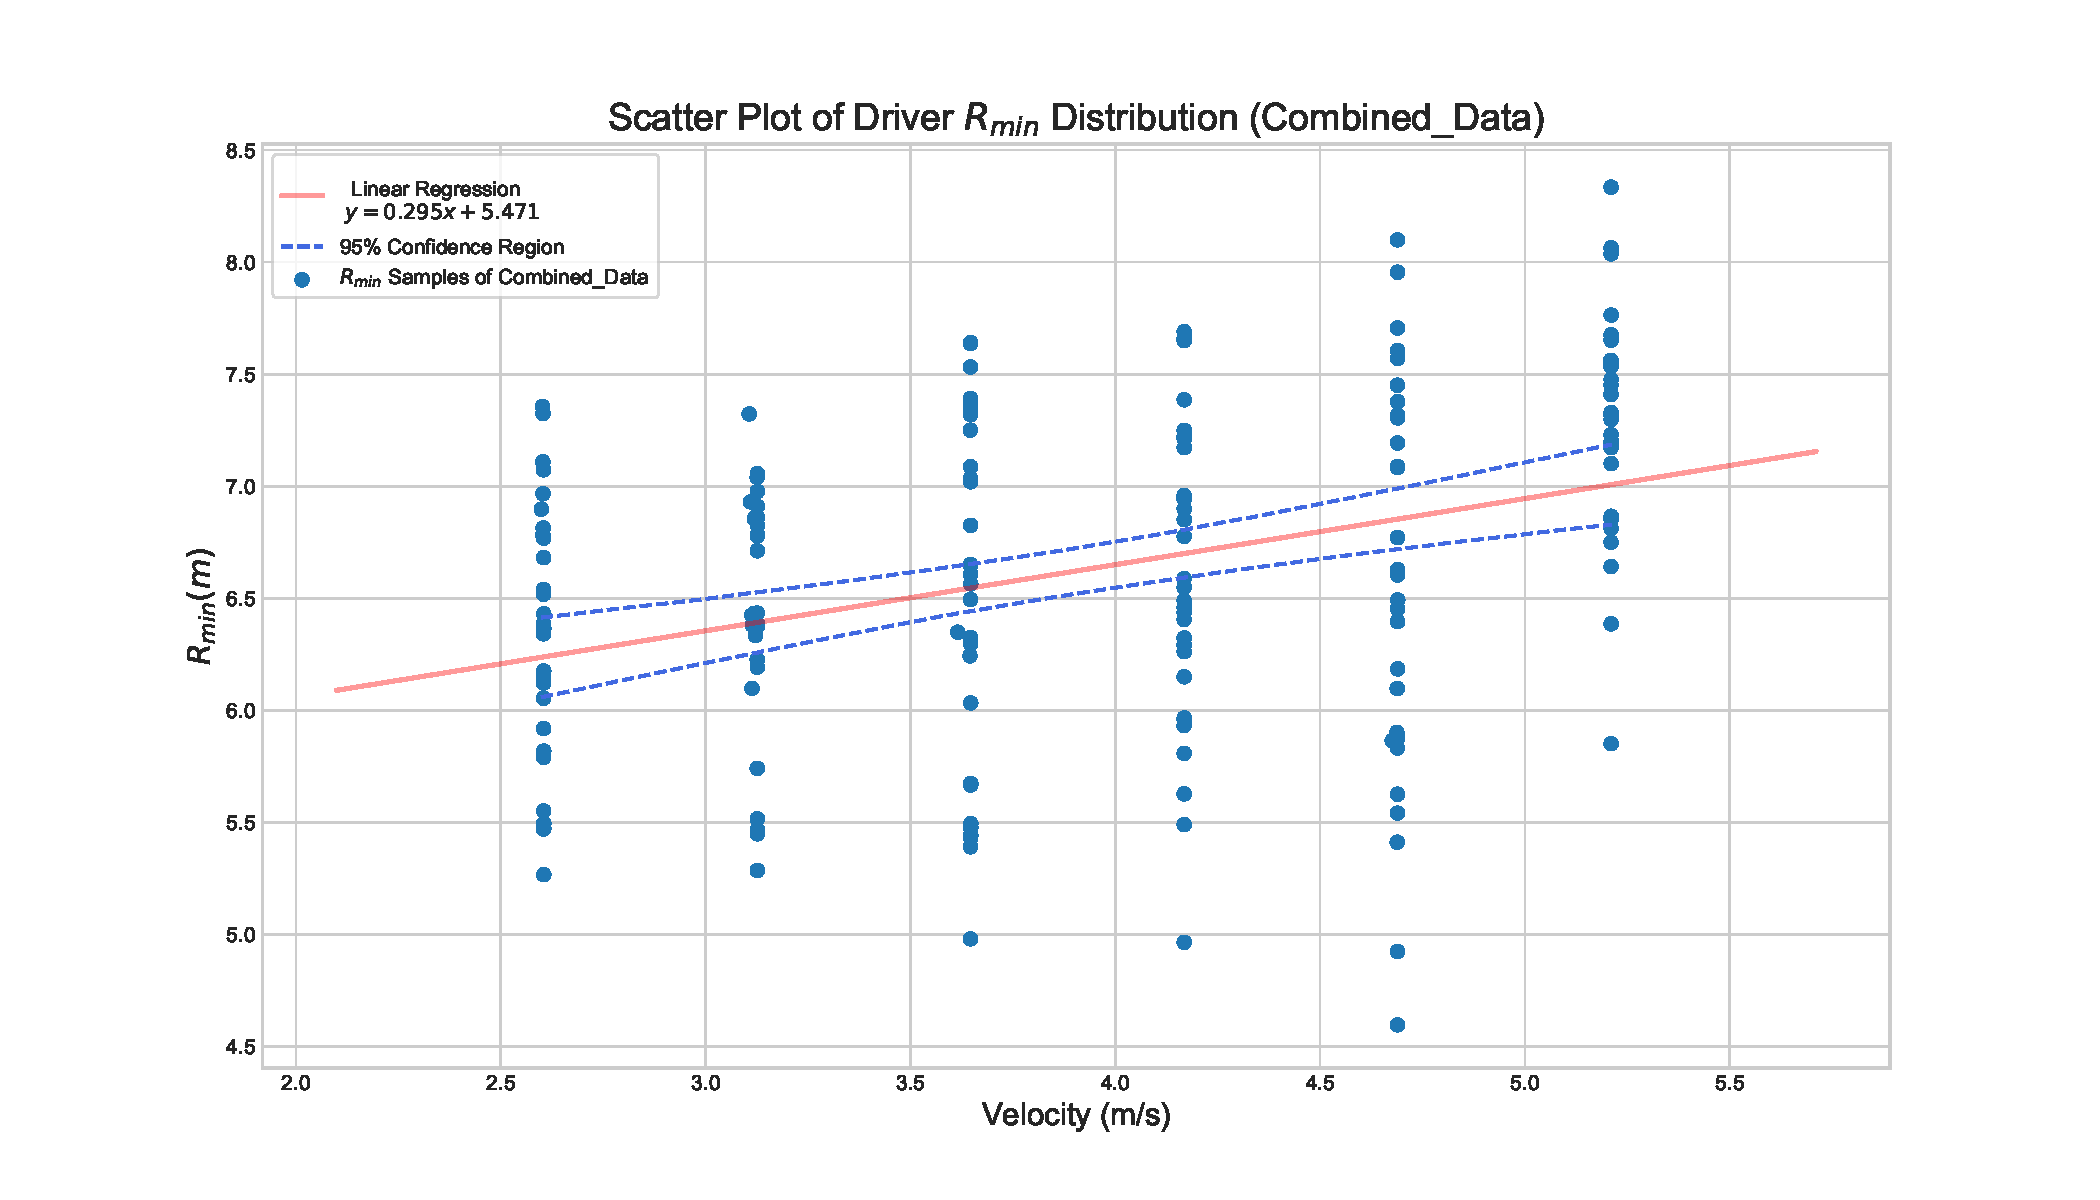
\includegraphics[width=0.7\paperwidth]{Combined_Data_R_MIN_polyfit.pdf}}
\end{center}
\caption{The $R_{min}$ scatter plot of combined data under various velocities.}
\label{fig:CombRMINDifSpeed} 
\end{figure}

\begin{figure}[htbp!]
\begin{center}
\makebox[0pt]{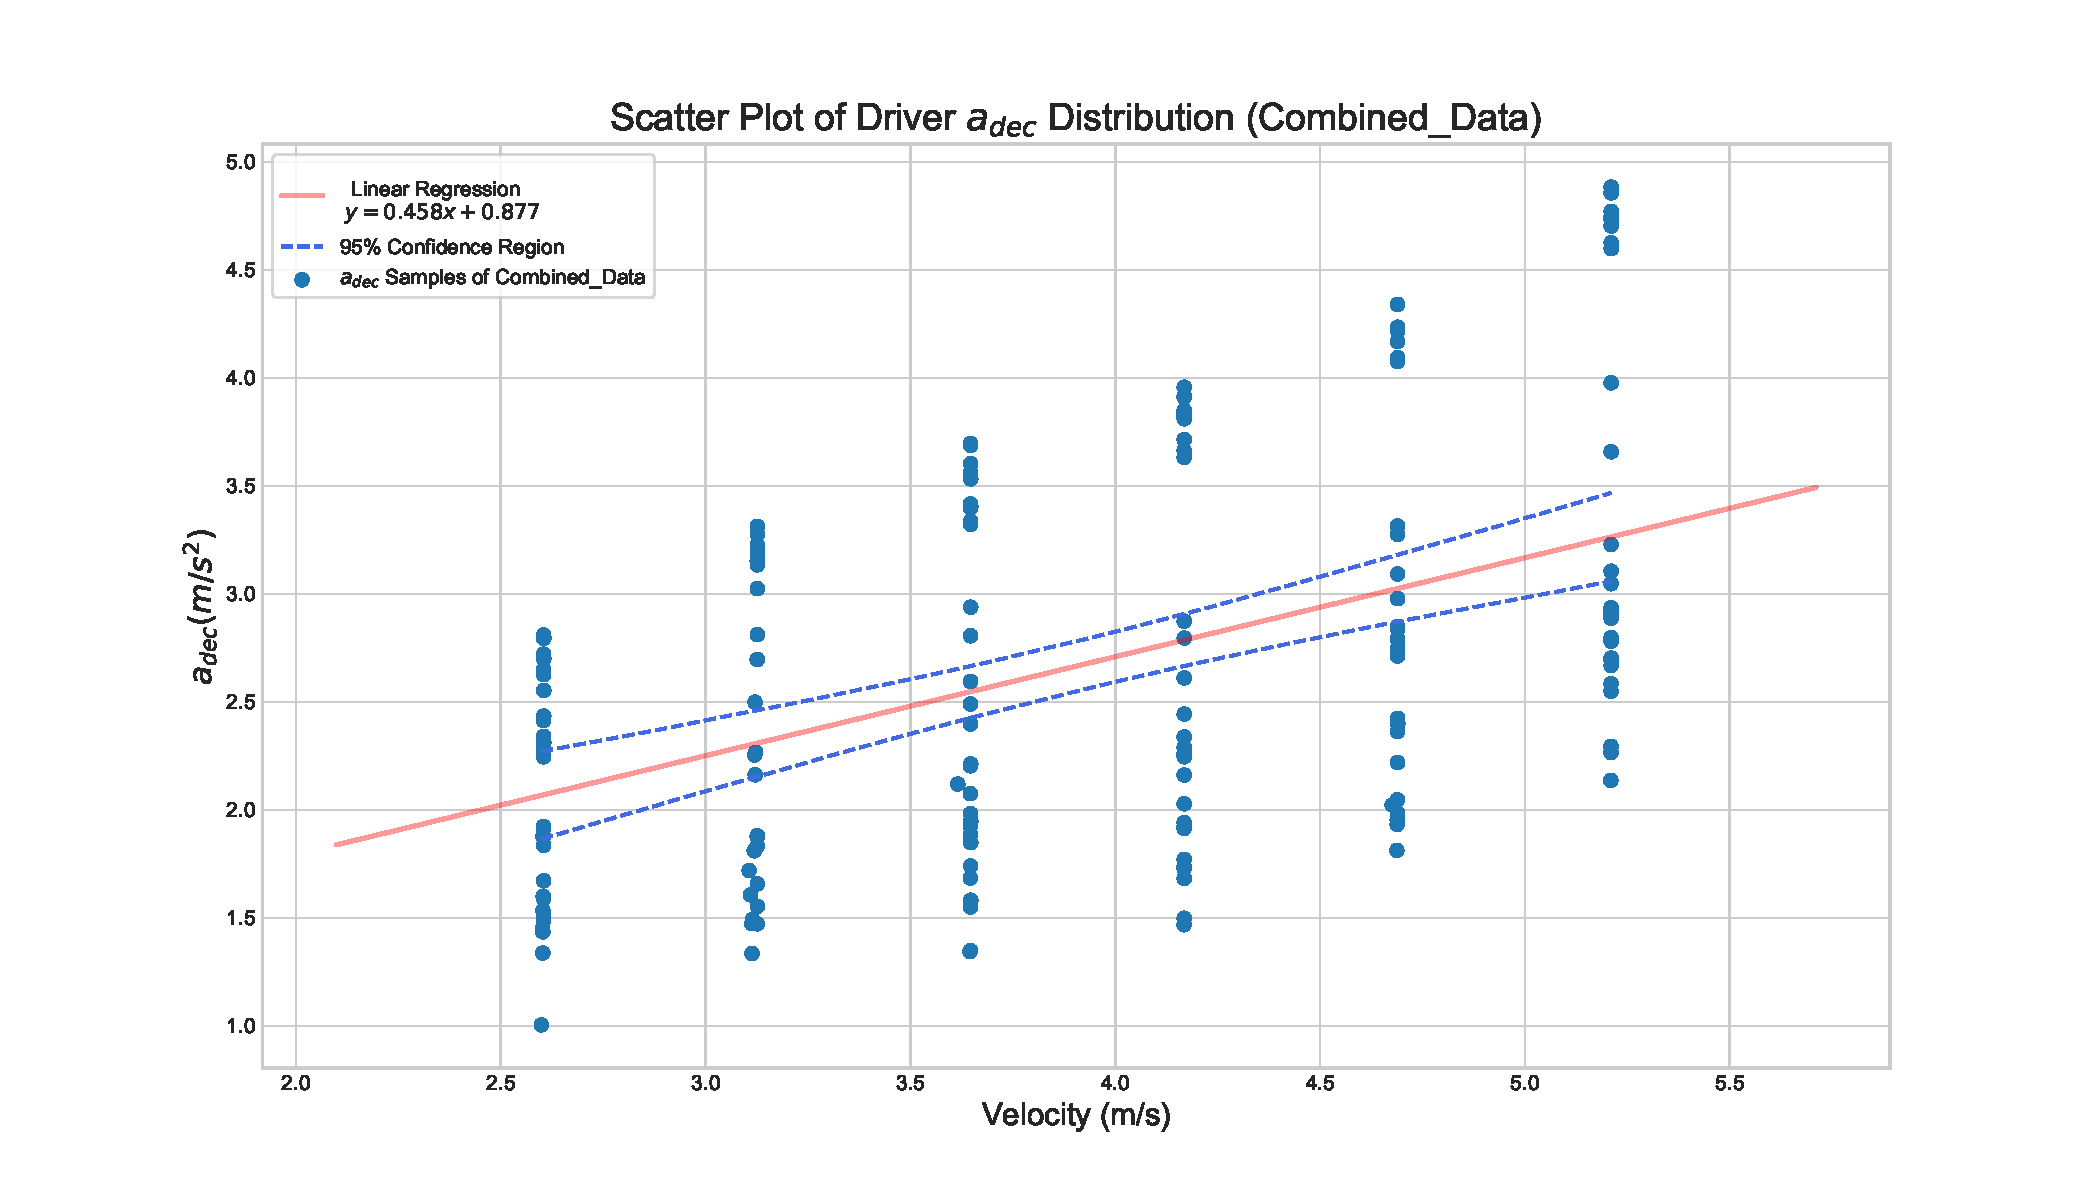
\includegraphics[width=0.7\paperwidth]{Combined_Data_A_DEC_polyfit.pdf}}
\end{center}
\caption{The $a_{dec}$ scatter plot of combined data under various velocities.}
\label{fig:CombADECDifSpeed} 
\end{figure}

\noindent where the approximated  equations for $R_{MIN}$ and $a_{dec}$ are

\begin{equation}
R_{min} = 0.295 v_i + 5.471
\label{eq:RMIN_Linear}
\end{equation}

\begin{equation}
a_{dec} = 0.458 v_i + 0.877
\label{eq:ADEC_Linear}
\end{equation}


We can see that the $R_{min}$ does get higher linearly as the velocity rises which is the same as predicted. The same trends happen to the $a_{dec}$ as the velocity ascends, which suggests that drivers brake slowly at low velocity and rapidly at high velocity. This is also reasonable since more urgent the situation is when the velocity is high. Therefore, the $R_{min}$ and $a_{dec}$ in Eqn.~\ref{eq:TFA_est} are also functions of $v_i$ which can be approximated by linear equation. Now we have all the elements needed, the required TFA distribution under different speed can now be estimated using ${TFA}_{est}$. Parameters used in the proposed TFA distribution estimation are listed in Table~\ref{table:parameters}. 

\begin{table}[htbp]
\caption{Table for parameters used in TFA distribution model.}
\begin{center}
\label{table:parameters}
\begin{tabular}{l l l l c}
& & \\ % put some space after the caption
\hline
\textbf{Parameters} &  & & &\textbf{Values} \\
\hline
Safe Margin Coefficient (${C1}_{Rmin}$)     &  &  & &  0.295  \\
Safe Margin Constant (${C2}_{Rmin}$)     &  &  & &  5.471  \\
Deceleration Coefficient (${C1}_{adec}$) &  &  & & 0.458  \\
Deceleration Constant (${C2}_{adec}$) &  &  & & 0.877  \\
Reaction Time ($\tau$)        &  &  & & 0.6 $s$ \\
Standard Diviation Parameter ($\gamma$)      &  &  & & 0.148  \\
\hline
\end{tabular}
\end{center}
\end{table}

\noindent where Safe Margin Coefficient (${C1}_{Rmin}$), Safe Margin Constant (${C2}_{Rmin}$), Deceleration Coefficient (${C1}_{adec}$), and Deceleration Constant (${C2}_{adec}$) standing for the coefficients and constants of the linear equation of $R_{min}$ and $a_{dec}$. $R_{min}$ and $a_{dec}$ are formulated in Eqn.~\ref{eq:RMIN_Linear} and Eqn.~\ref{eq:ADEC_Linear}.

\begin{equation}
R_{min} = {C1}_{Rmin} v_i + {C2}_{Rmin}
\label{eq:RMIN_Linear}
\end{equation}

\begin{equation}
a_{dec} = {C1}_{adec} v_i + {C2}_{adec}
\label{eq:ADEC_Linear}
\end{equation}

Finally, the model to estimate the TFA distribution of general people is completed. The TFA distributions are proved to be normally distributed and the formulated $TFA_{est}$ can also account for the hyperbolic growth in the TFA data collected. In the next section, the TFA distribution will be used as the core of the proposed probabilistic model.

%%%%%%%%------------------------------%%%%%%%%%
%%%%%%%%-----------SUBSECTION---------%%%%%%%%%
%%%%%%%%------------------------------%%%%%%%%%
\subsection{The Model for Probability of Yielding Estimation}
So far, the problem concerning the model for TFA distribution is solved by considering the distance needed for the driver to yield. Then the distance is divided by the speed at the instance and turned into the ${TFA}_{est}$. Before the TFA distribution is brought into the probability evaluation method proposed in section \ref{sub:TFA PDF}, few improvements are required because the proposed model is unable to account for all the situations yet. 

For example, the situation where a vehicle is accelerating through the node is described in Fig.~\ref{fig:TTC_acc}. Three sub-figure from the top to the bottom are the velocity, the displacement to the node and the TTC versus the time respectively. Note that in this example, the acceleration of the vehicle is constant, so the line of velocity rise linearly while the displacement to the node and TTC are a parabolic and the curve consisting of reciprocal and linear function separately. In this figure, as the velocity of the vehicle is accumulating, the displacement to the node drops in a parabolic curve since the vehicle is moving closer. The resulting TTC curve, defined by Eqn.~\ref{eq:TTC_crossroad}, is also decreasing and even goes beneath 0. In the cases like this one, the POY using merely the integral from the TFA distribution, as in Fig.~\ref{fig:TTC_distribution}, would causing the increase of the POY as the TTC keeps decreasing.

\begin{figure}[htbp!]
\begin{center}
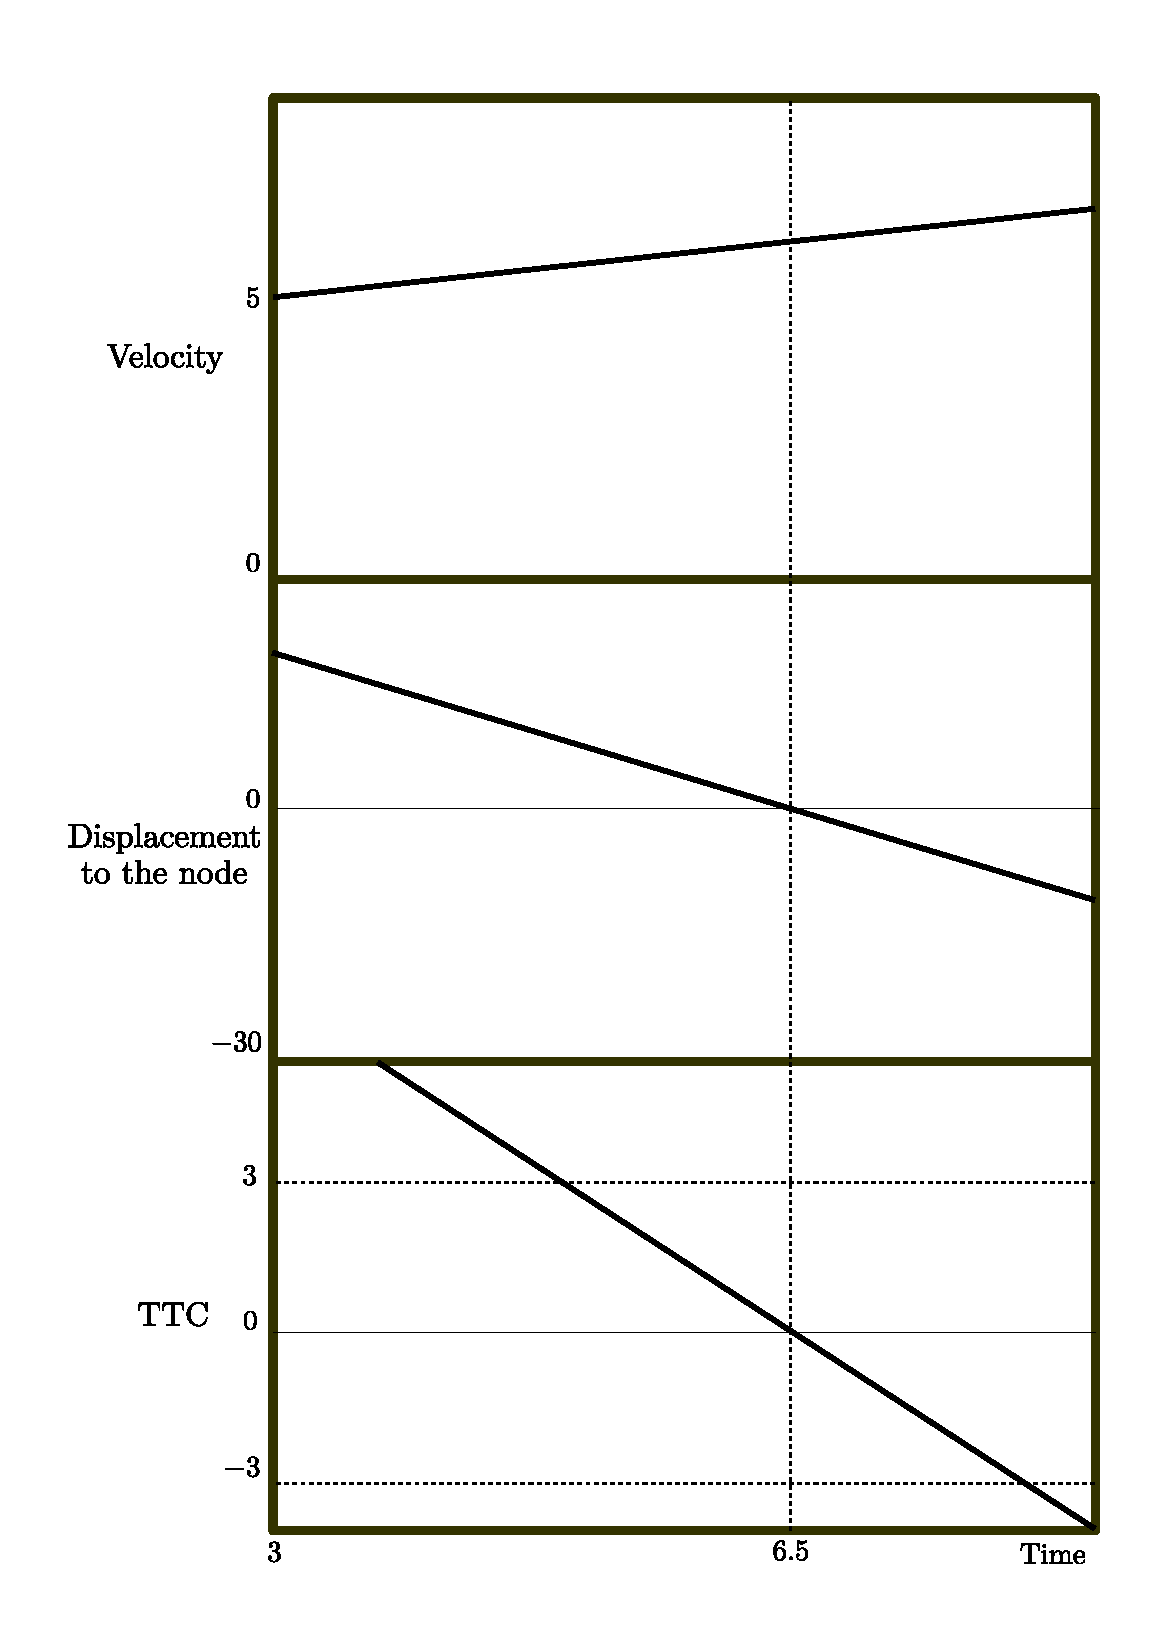
\includegraphics[scale=0.6]{TTC_change_when_accelerating.pdf}
\end{center}
\caption{History of TTC as the vehicle accelerating through the node.}
\label{fig:TTC_acc} 
\end{figure}

To overcome this problem, few adjustments are needed to be performed. First, the influence of the acceleration on the probability of stopping should be considered. As described in the above example, besides the integral acquired from the TFA distribution, the current states of acceleration are also important. After some trials for different possibilities, the first order derivative of TTC is chosen. By assuming constant acceleration while braking, the $d_{node, i, t}$ can be expressed as

\begin{equation}
d_{node, i, t} = d_{node,i,0} - \biggl(v_0t+\frac{1}{2}at^2\biggr)
\label{eq:d_node}
\end{equation}

\noindent where $d_{node,i,0}$ is the displacement at the beginning of the brake, $v_0$ is the speed and $a$ the acceleration. Then, combining Eqn.~\ref{eq:d_node} and Eqn.~\ref{eq:TTC_crossroad}, the derivative of TTC is determined

\begin{equation}
TTC' = \frac{d}{dt}\frac{d_{node,i,t}}{v_t} = -1 -a \cdot d_{node,i,t} \cdot v_t^{-2}
\label{eq:TTC'}
\end{equation}

As a dimensionless weighting parameter, $TTC'$ takes not only acceleration but also displacement and the speed into account. For instance, when a constant deceleration is applied, the higher the speed of the vehicle implies the smaller chance this vehicle will yield and vice versa. So this weighting parameter is capable of punishing those with low TTC while accelerating or at high speed and rewarding those with deceleration or low speed. Now, the last step is to add this weighting on the proposed model. 

In order to increase the POY in those circumstances such as the deceleration or the low vehicle speed, the mean value of ${TFA}_{est}$ should is elevated. Similarly, to decrease the POY while the vehicle is accelerating or driving with high speed, the mean value of ${TFA}_{est}$ is reduced. However, chances are the brake is not applied to yield but to adjust the speed, or it is not acceleration but simply some sensor errors, which all could lead to bumpy probabilities of yielding. To bring down the number of the results affected by false positive, the following adjustments are made


\begin{equation}
    P_{yield, t} = \Bigr(1-\Phi_{\mu, \sigma^{2}}\big({min TTC}_{t}\big)\Bigl)
\label{eq:POY}
\end{equation}

where  $P_{yield, t}$ is the proposed probability of yielding at time $t$, $\Phi_{\mu, \sigma^{2}}$ is the CDF of the TFA distribution $\mathcal{N}(\mu,\sigma^{2})$, $\mu$ is defined by ${TFA}_{est, t} + A_{t}$ which represents the adjusted mean value of the TFA distribution and $\sigma_{est, t}$ is the resulting adjusted mean value of the TFA distribution.

The weighting parameter $A_{t}$ is defined as

\begin{equation}
    A_{t} = 
    \begin{cases} 
      \alpha_{t} &~~\text{if}~~ \lvert \alpha - \alpha_{t-1}  \rvert < 1.67 \cdot \sigma_{est, t}\\
      1.67 \cdot \sigma_{est, t} &~~\text{otherwise}
    \end{cases}
\label{eq:alpha_cap}
\end{equation}

\noindent where $\alpha_t$ in Eqn.~\ref{eq:alpha_cap} is dominated by the acceleration. From Eqn.~\ref{eq:TTC'}, we can see that the $TTC'$ equals -1 when the acceleration is 0. So the $TTC'$ value is greater than -1 when the subject vehicle is decelerating, and less than -1 when accelerating. In order to account for the acceleration as well as the velocity, $\alpha_t$ is defined as 

\begin{equation}
    \alpha_{t} = 
    \begin{cases} 
      \beta_{t} \cdot \ln \left ( ~ \left( ~ \lvert {TTC'}_{t}  \rvert + 1 ~\right) \cdot e~ \right) &~~\text{if}~~ {TTC'}_{t} > -1\\
      - \beta_{t} \cdot \ln \left ( ~ \left( \lvert {TTC'}_{t}  \rvert + 1 \right) \cdot e~ \right) &~~\text{if}~~ {TTC'}_{t} < -1 \\
      \alpha_{t-1} &~~\text{otherwise}
    \end{cases}
\label{eq:alpha}
\end{equation}

\noindent where

\begin{equation}
    \beta_{t} = 
     \max ~ \big( ~ \lvert {min TTC}_{t} - TFA_{est, t} \rvert, ~ \sigma_{est, t} ~ \big)
\label{eq:beta}
\end{equation}



As describe in Eqn.~\ref{eq:POY}, the weighting $A_t$ is applied to increase the mean value of the TFA distribution. When the $A_t$ is positive, meaning that the POY will increase under the same TTC, which is due to the larger integral of that area under TFA distribution, and vice versa for the negative $A_t$ valaues. This is illustrated in Fig.~\ref{fig:TFA_weighting_before} and Fig.~\ref{fig:TFA_weighting_after}. In Fig.~\ref{fig:TFA_weighting_before}, the current TTC equals the mean of the TFA distribution so the resulting POY is 0.5 . However, since the vehicle is decelerating, the mean value of the TFA distribution is adjusted according to Eqn.~\ref{eq:alpha}. The POY, which is the area under the TFA distribution and right to the current TTC, becomes 0.97, as illustrated in Fig.~\ref{fig:TFA_weighting_after}.

\begin{figure}[htbp!]
\begin{center}
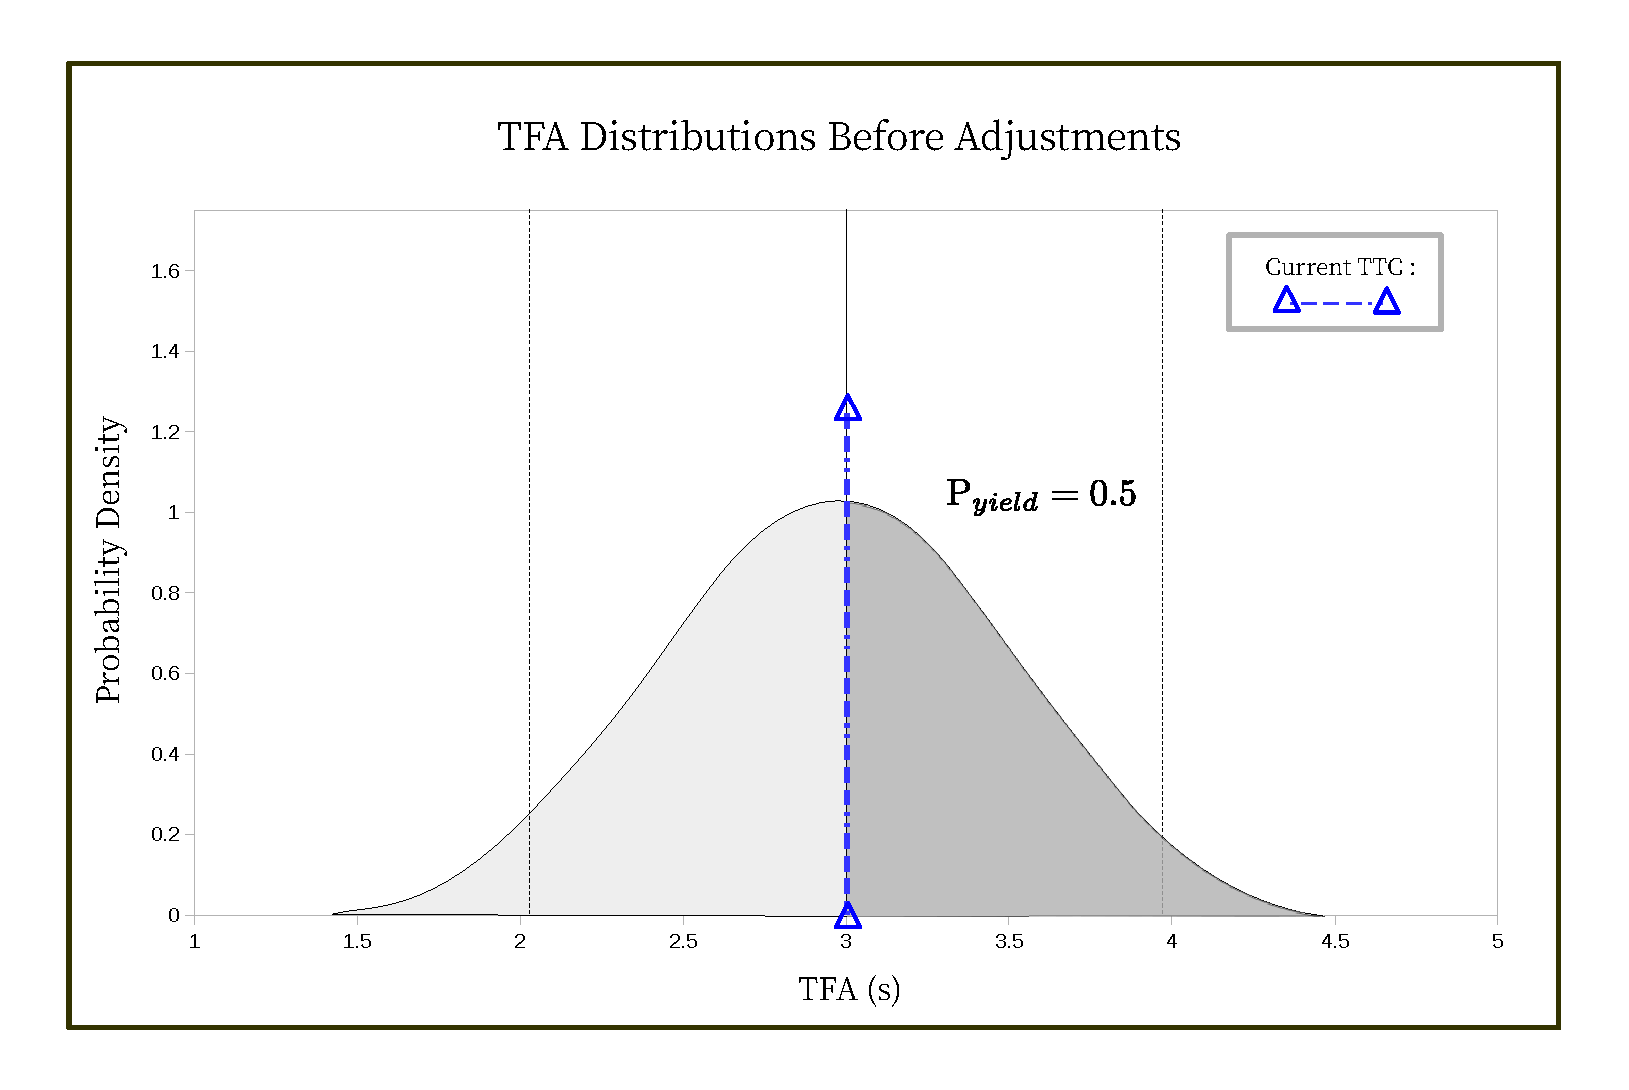
\includegraphics[scale=0.4]{TFA_weighting_before.pdf}
\end{center}
\caption{The probability before the weighting parameter $A_t$ is 0.5 .}
\label{fig:TFA_weighting_before} 
\end{figure}

\begin{figure}[htbp!]
\begin{center}
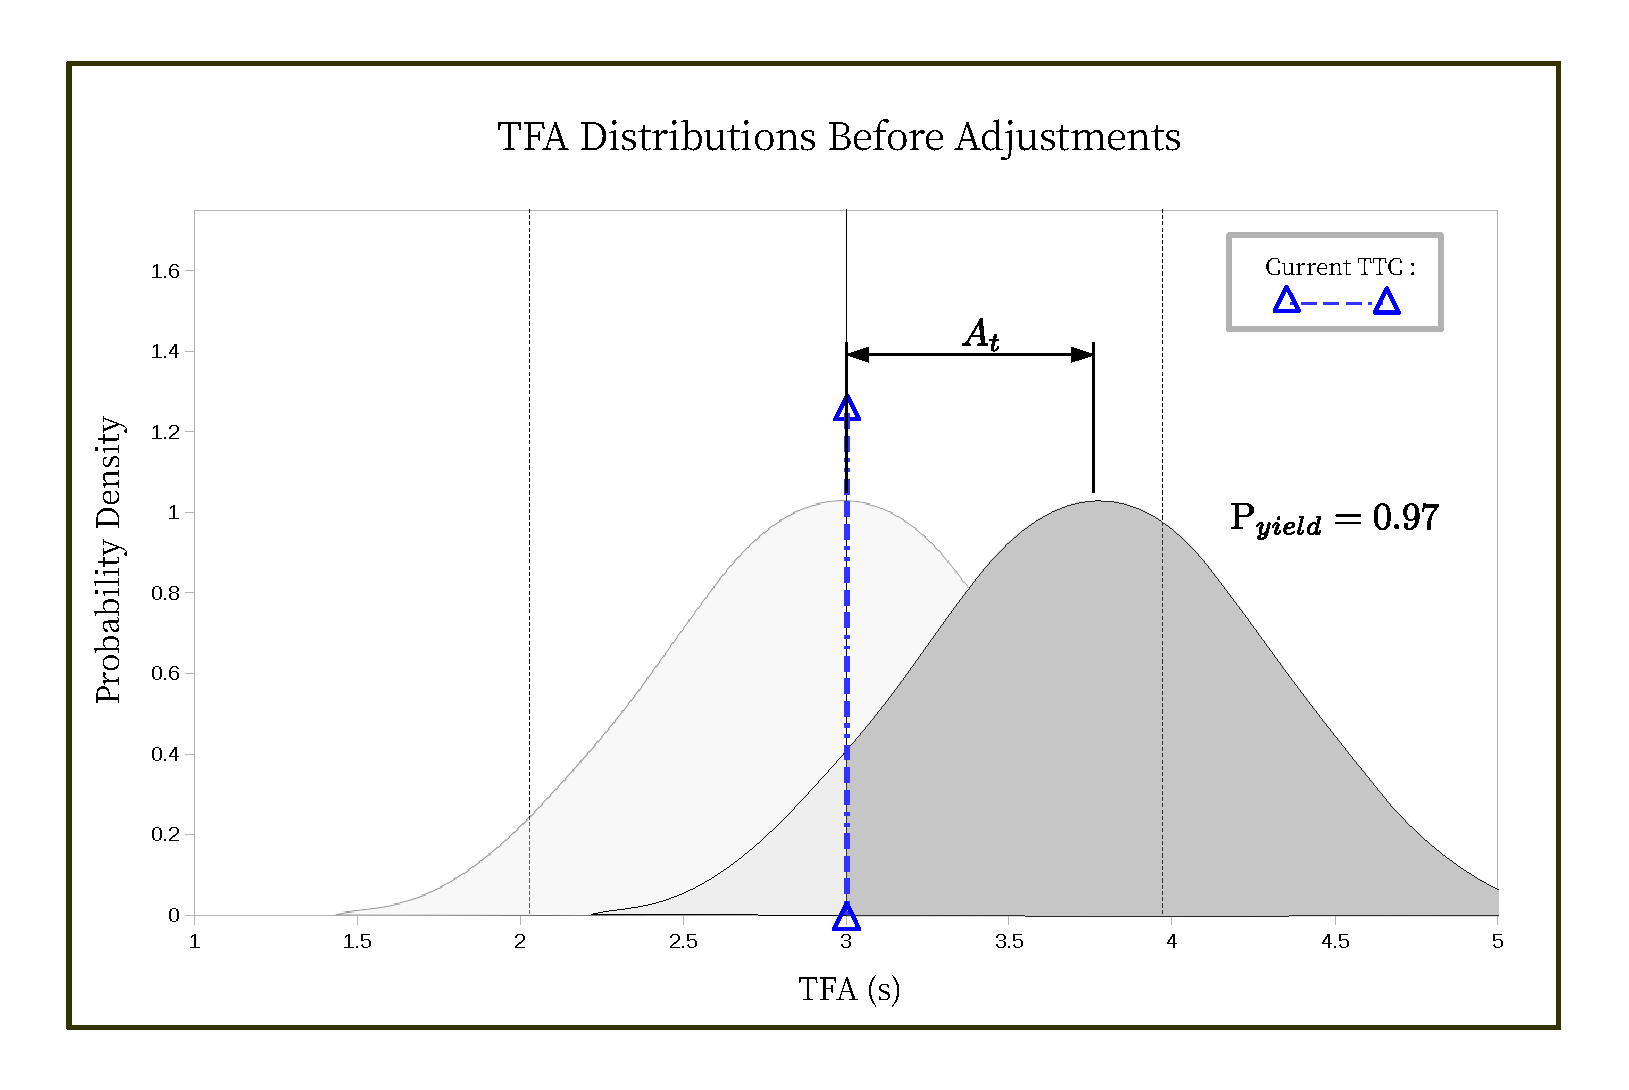
\includegraphics[scale=0.4]{TFA_weighting_after.pdf}
\end{center}
\caption{The probability after the weighting parameter $A_t$ is 0.97 .}
\label{fig:TFA_weighting_after} 
\end{figure}

In Eqn.~\ref{eq:alpha}, the magnitude of $\alpha_t$ is adjusted depending on the greater one between $\lvert {min TTC}_{t} - TFA_{est, t} \rvert $ and $ \sigma_{est, t}$ (as shown in Eqn.~\ref{eq:beta}). By doing so, the increase or decrease of the mean value of the TFA distribution will be in direct proportion to the difference between ${min TTC}_{t}$ and $TFA_{est, t}$ if $\lvert {min TTC}_{t} - TFA_{est, t} \rvert $ is larger. Within those situation where the $\lvert {min TTC}_{t} - TFA_{est, t} \rvert $ is too small or even equals to 0, $ \sigma_{est, t}$ is used instead. Either way, the resulting $\beta_{t}$ value allows the proposed model to have more immediate response to the situation at the moment. ( Noted that in Eqn.~\ref{eq:alpha}, $\lvert {TTC'}_{t} \rvert$ in both conditions are added by 1 and times $e$, so the outcome of the natural logarithm will be greater than 1 at all times. )

However, jagged POY curve might be shown if the response is "too immediate", in other word, if the value of $\alpha_t$ is too large, the resulting POY curve would be too cluttered. For example, if the current POY is 0.97 as depicted in Fig.~\ref{fig:TFA_weighting_after}, and the $\alpha_t$ at the moment is minus four standard deviation. In the next moment, the POY then drop rapidly from 0.97 to 0.0 . If situations like this keep repeating, there will be too many spikes for people to understand the real intention of the other driver. As a result, the maximum value of $A_t$ is set to 1.67 standard deviation to suppress the value and prevent the POY from rising or dropping too rapidly.  

Another reason for spikes on the POY curves is that, the throttles or brakes are sometimes applied for speed adjustments, not yielding or passing. To prevent the POY curve from making response to situations like this, the change of sign in $A_t$ would only be accepted when the acceleration introducing the change last for longer than 0.2 sec, i.e., when the vehicle starts braking, the $A_t$ brought by this brake would only be applied when the deceleration lasts longer than 0.2 sec. Even though the sensitivity to the yielding or passing cases might be diminished if the threshold is set too large, this can effectively reduce the number of cases falsely detected as the other intention. 

Up till now, the driver behaviors at the crossroad is modeled in a probabilistic way. The proposed probabilistic of yielding is able to anticipate the decision of drivers at the crossroad. With this functionality, the proposed method can help autonomous vehicle to understand the intentions of other traffic participants and make the mixed-fleet safer before the fully autonomous vehicles are adopted by 100\%.

The intents of drivers at simulated and real crossroad are predicted and shown using the proposed model. Then, the verification is conducted using the classification accuracy rate, and the results are also compared with other methods from the literature. 


%%%%%%%%%%%%%%%%%%%%%%%%%%%%%%%%%%%%%%%%%%%%%%%%%%%%%%%%%%%%%%%%%%%%%%%%
%%%%%%%%%%               SECTION SECTION SECTION               %%%%%%%%%
%%%%%%%%%%%%%%%%%%%%%%%%%%%%%%%%%%%%%%%%%%%%%%%%%%%%%%%%%%%%%%%%%%%%%%%%
\section{Driver Intentions Prediction with Probability of Yielding}
\label{sec:ValidatePOY}

In Section \ref{sec:POY}, the \ac{POY} is proposed to evaluate the intentions of drivers at crossroads probabilistically. To verify the outcomes of the proposed model, experiments are conducted in both virtual and real environments. The states required in the proposed model are extracted from the data and send into the model. Finally, the predicted behaviors are compared to the actual behaviors and the discussion is also made.

%%%%%%%%------------------------------%%%%%%%%%
%%%%%%%%-----------SUBSECTION---------%%%%%%%%%
%%%%%%%%------------------------------%%%%%%%%%
\subsection{Urban Crossroads in Simulated Environment}
\label{sub:simulated env}

The simulated environment (as shown in Fig.~\ref{fig:GazeboCrossroad}) is constructed in Gazebo which is an open source, 3 dimensions robotics simulator. Gazebo has been used in varius technical challenges and competitions including DARPA Robotics Challenge (2012-2015), NASA Space Robotics Challenge (2016-2017) and Toyota Prius Challenge (2016-2017). This simulator is known for its accuracy and the powerful, robust physics models that can simulate the world to the extent that most of the data output required for the model is available. Despite only the displacement from the subject vehicle to the the node and the speed of the vehicle is required, the realistic rendering of the constructed environment can minimize the differences between virtual and real crossroads. Also, here are a few advantages of using simulated world. First, collecting the data from experiments becomes easier. The required states of targets can be directly extracted form the simulator. Second, different scenarios can be employed with little efforts. Thirdly, it is both time and cost efficient.

\begin{figure}[htbp!]
\begin{center}
\makebox[0pt]{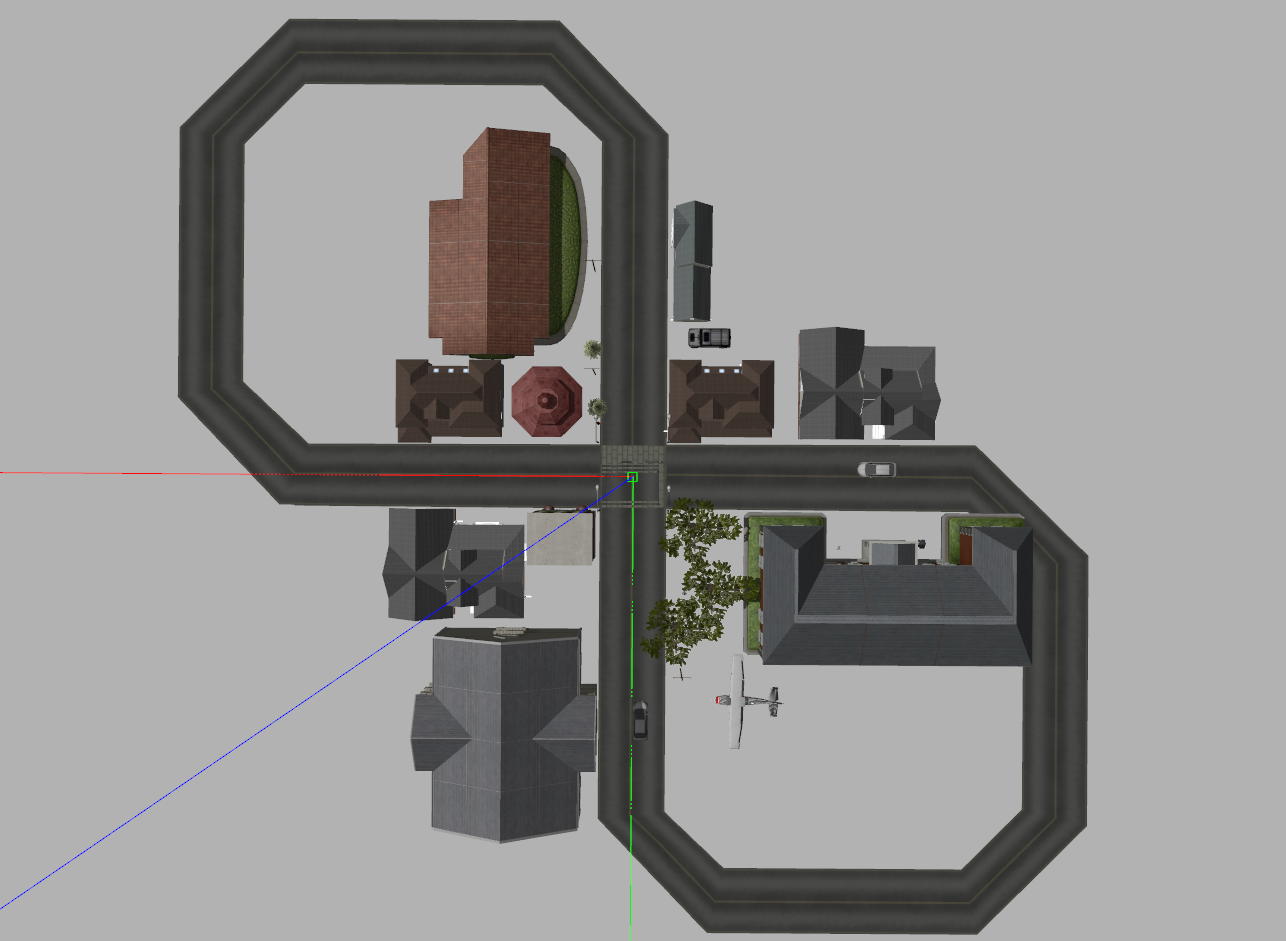
\includegraphics[width=0.7\paperwidth]{GazeboCrossroad.png}}
\end{center}
\caption{The simulated crossroad scenario in the Gazebo simulator.}
\label{fig:GazeboCrossroad} 
\end{figure}

The simulated vehicle in the virtual world are controlled using Gazebo ROS Controller which is a part of ROS packages names gzebo\_ros\_pkgs. This package provide the necessary modules and interfaces to simulate a robot (a vehicle in our case) in Gazebo which is taking orders from ROS messages and services. ROS is the short for "Robot Operating System" which is a robotics middleware that provide users with integrated packages, services and tools. The reusability for codes, implemented in multiple languages and continuous support from its community are all the benefits of ROS. 


The front, left and right views from the driver seat are directly projected onto the screens when driving in simulated world. (Fig.~\ref{fig:FrontCam}, Fig.~\ref{fig:LeftCam} and Fig.~\ref{fig:RightCam} respectively.) Control commands from the volunteers are sent from the joysticks to ROS node (a single process under ROS). Then the command velocity calculated according to the movement of the joystick is finally sent from the ROS node to the simulated vehicle in Gazebo. In every set of interaction experiments, a pair of volunteers (as shown in Fig.~\ref{fig:Driver1} and Fig.~\ref{fig:Driver2}) are asked to drive across the intersection without collision. The displacements to the node and the speed of vehicles for both driver are recorded with the time resolution of 0.01 sec. 

\begin{figure}[htbp!]
\begin{center}
\makebox[0pt]{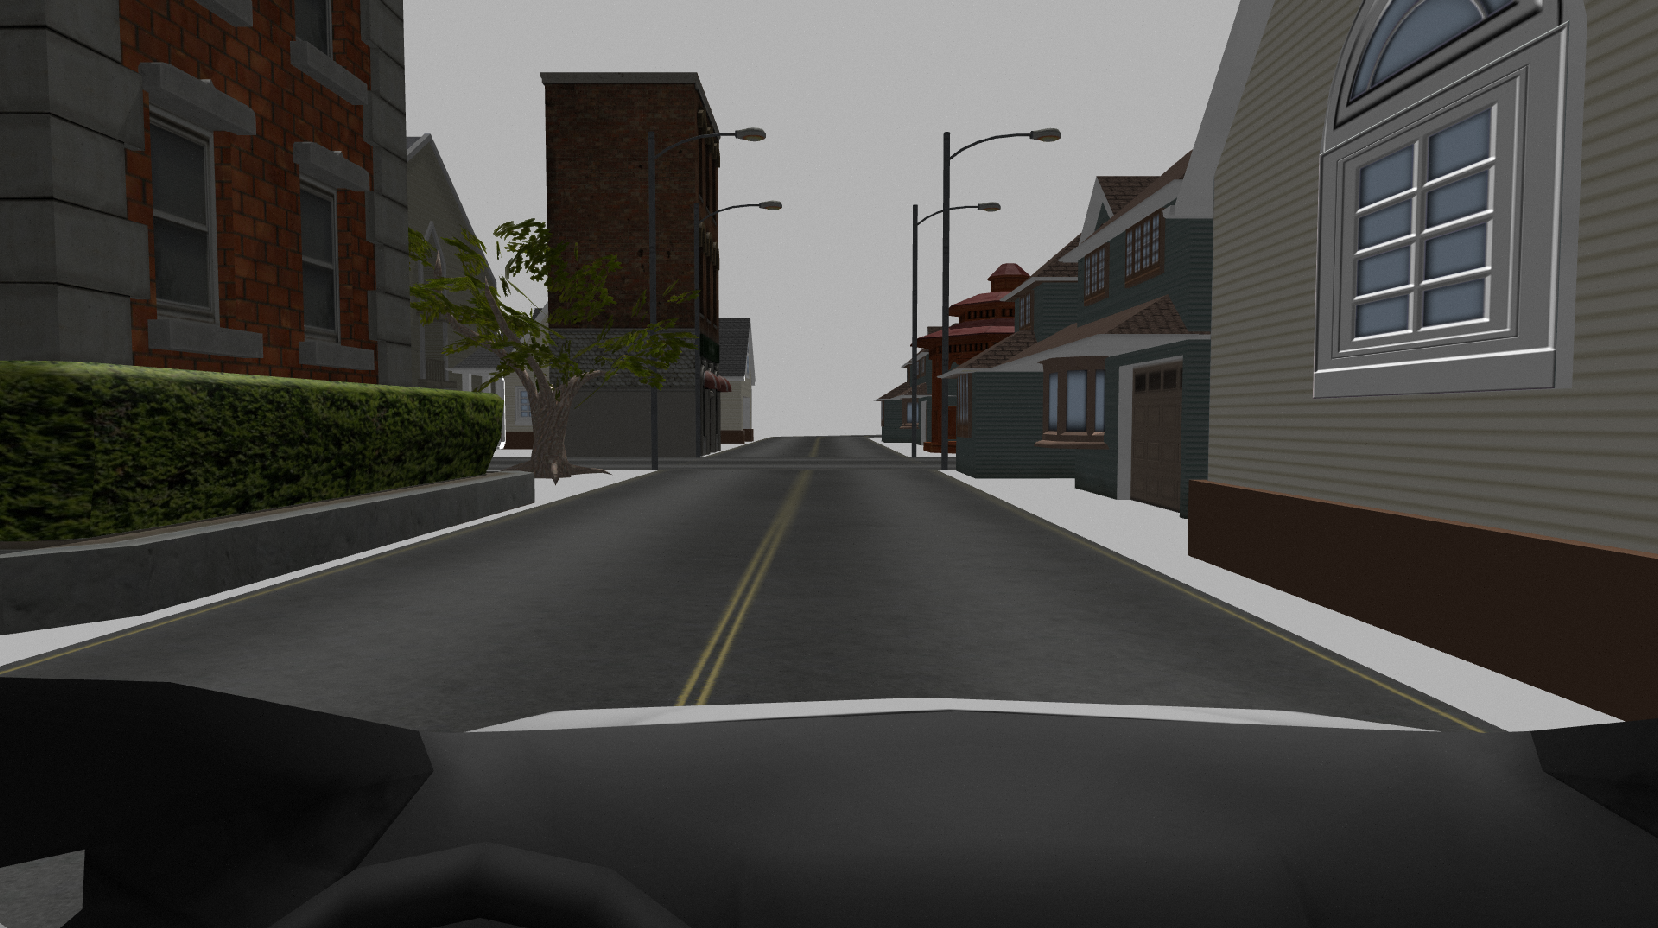
\includegraphics[width=0.7\paperwidth]{PriusFcam.png}}
\end{center}
\caption{Front camera from driver seat in the simulated environment.}
\label{fig:FrontCam} 
\end{figure}

\begin{figure}[htbp!]
\begin{center}
\makebox[0pt]{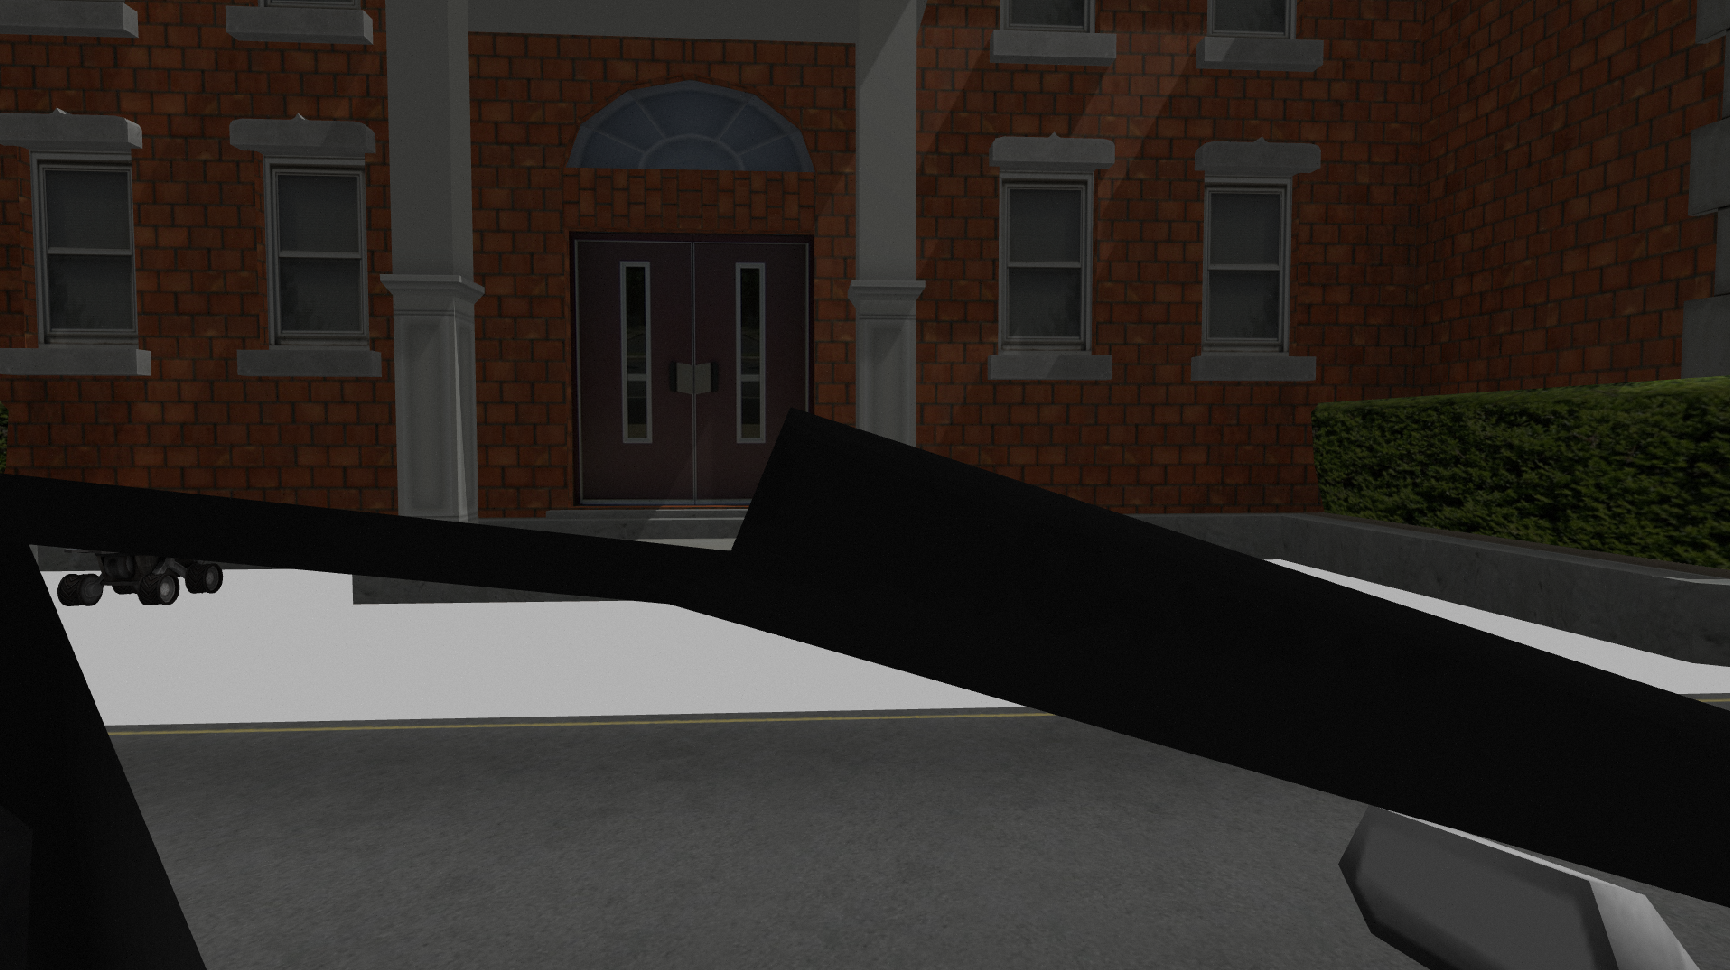
\includegraphics[width=0.7\paperwidth]{PriusLcam.png}}
\end{center}
\caption{Left camera from driver seat in the simulated environment.}
\label{fig:LeftCam} 
\end{figure}

\begin{figure}[htbp!]
\begin{center}
\makebox[0pt]{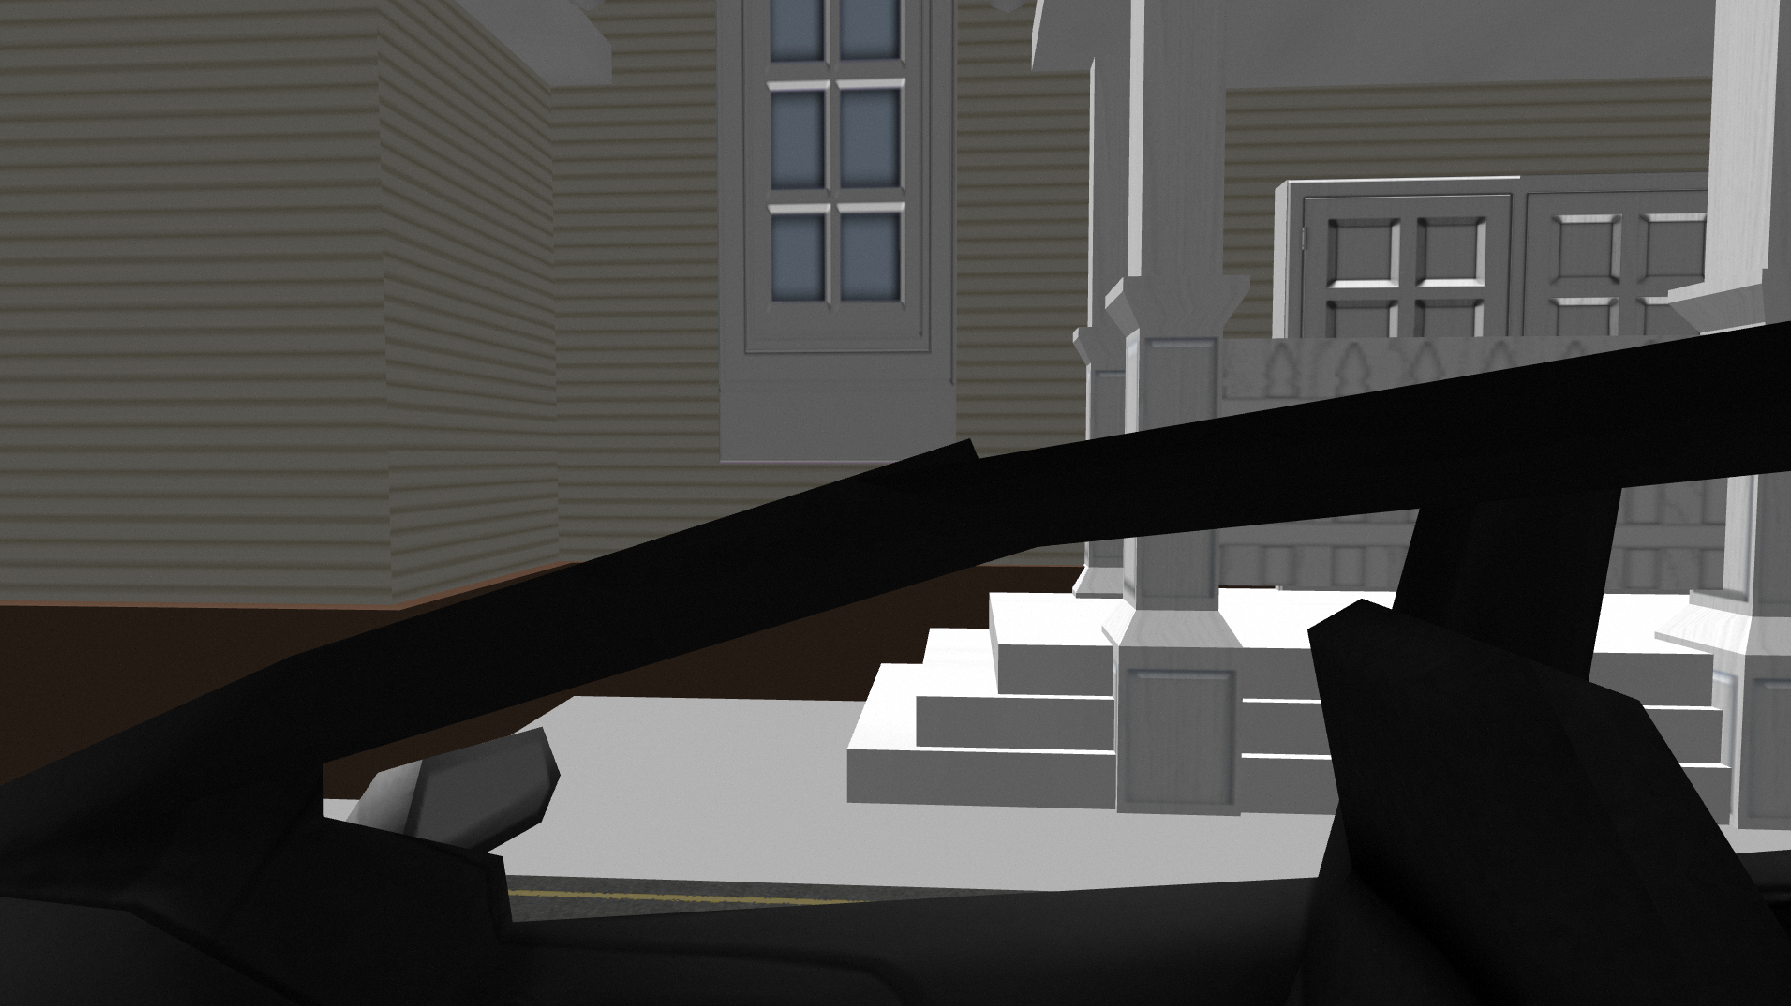
\includegraphics[width=0.7\paperwidth]{PriusRcam.png}}
\end{center}
\caption{Right camera from driver seat in the simulated environment.}
\label{fig:RightCam} 
\end{figure}

\begin{figure}[htbp!]
\begin{center}
\makebox[0pt]{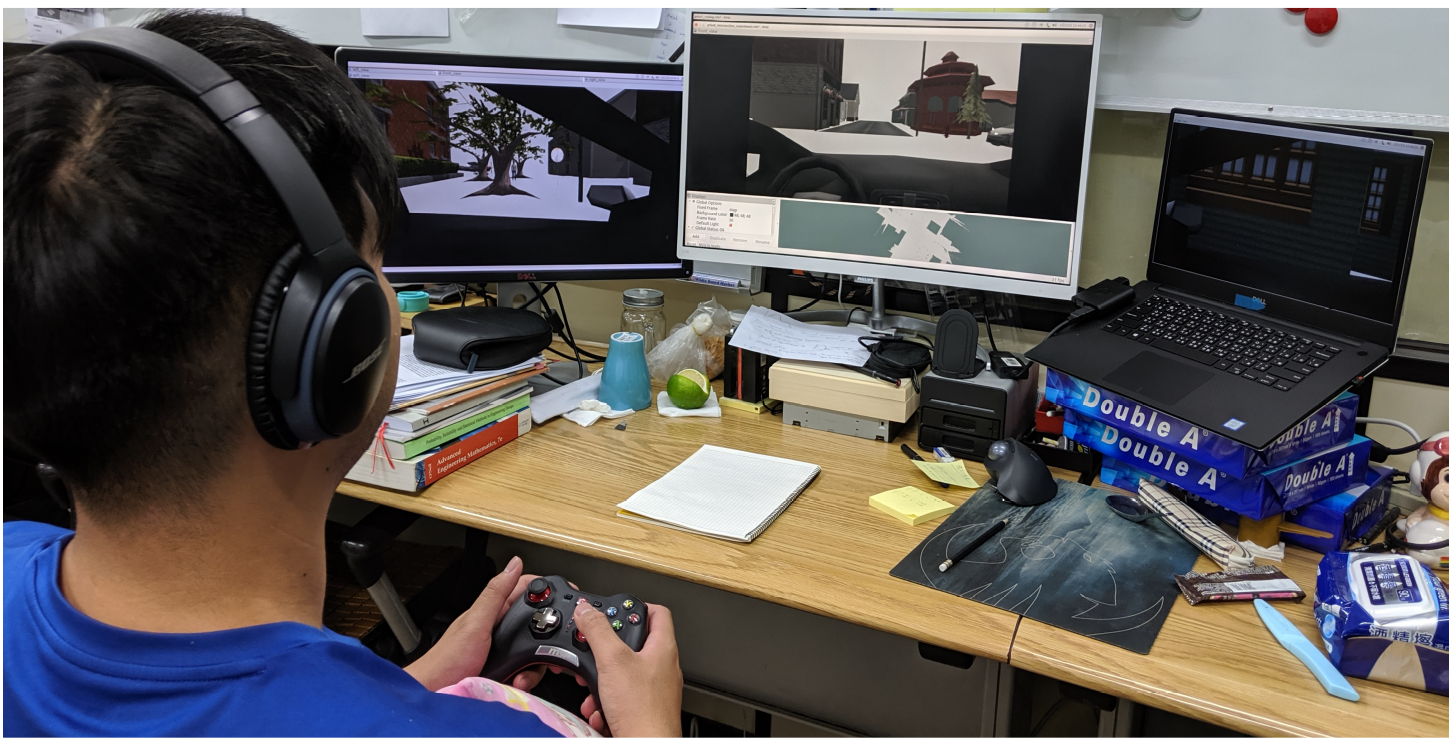
\includegraphics[width=0.7\paperwidth]{Driver1.png}}
\end{center}
\caption{First driver in the simulated crossroad interaction experiment.}
\label{fig:Driver1} 
\end{figure}

\begin{figure}[htbp!]
\begin{center}
\makebox[0pt]{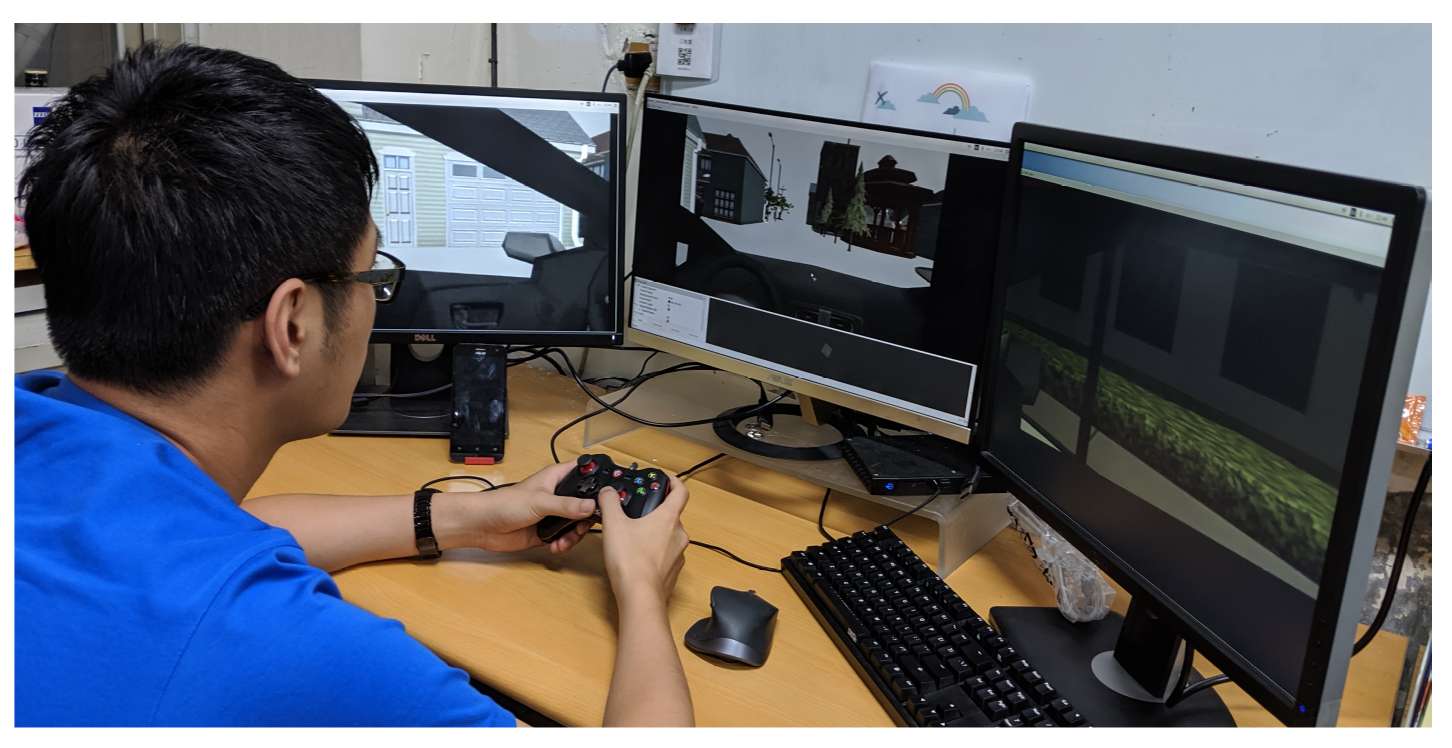
\includegraphics[width=0.7\paperwidth]{Driver2.png}}
\end{center}
\caption{Second driver in the simulated crossroad interaction experiment.}
\label{fig:Driver2} 
\end{figure}

%%%%%%%%------------------------------%%%%%%%%%
%%%%%%%%-----------SUBSECTION---------%%%%%%%%%
%%%%%%%%------------------------------%%%%%%%%%
\subsection{Experimental Results in Simulated Environment}
\label{sub:ResultSim}

Since there are three participants who are asked to participate in pair, and about 50 repetitions were conducted each pair, so there will be about 150 sets of data in total. Within these trials, some will be explained in detail to demonstrate the performance of the proposed model. Then the classification accuracy rate will be evaluated using all data sets for validation.  

\begin{figure}[htbp!]
    \centering
    \subfloat[Illustration of calculated TTC of each vehicle.]
    {
    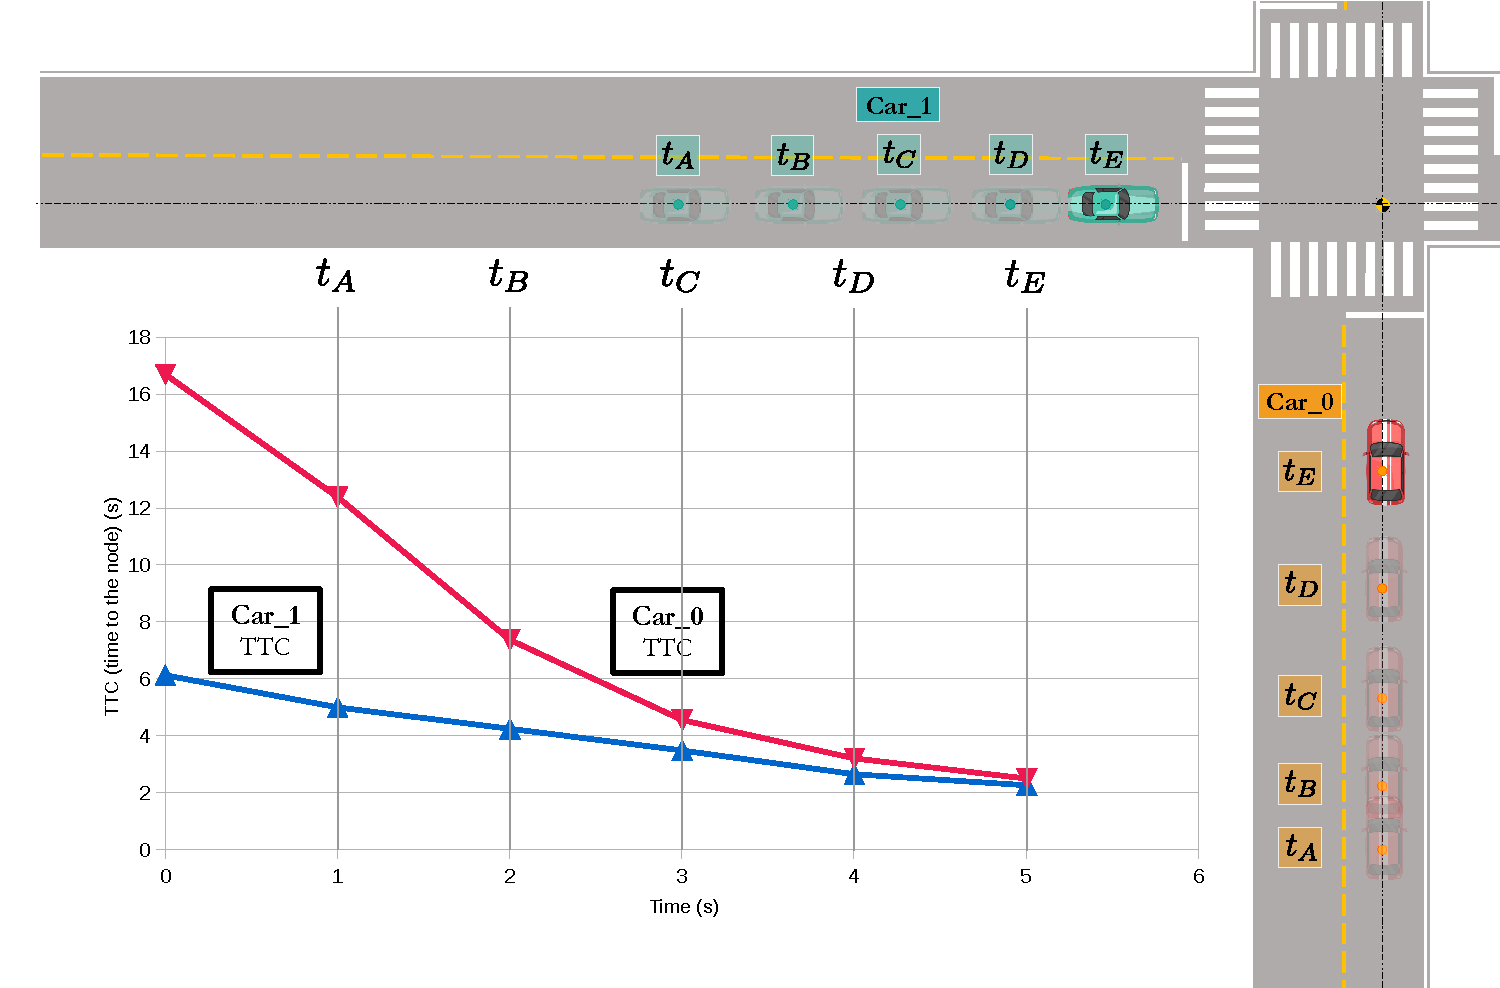
\includegraphics[width=0.47\textwidth]{figure_explaination_TTC.pdf}
    \label{fig:figure_explaination_TTC}
    }\hfill
    \subfloat[Illustration of probability of stopping together with velocity and displacement.]
    {
    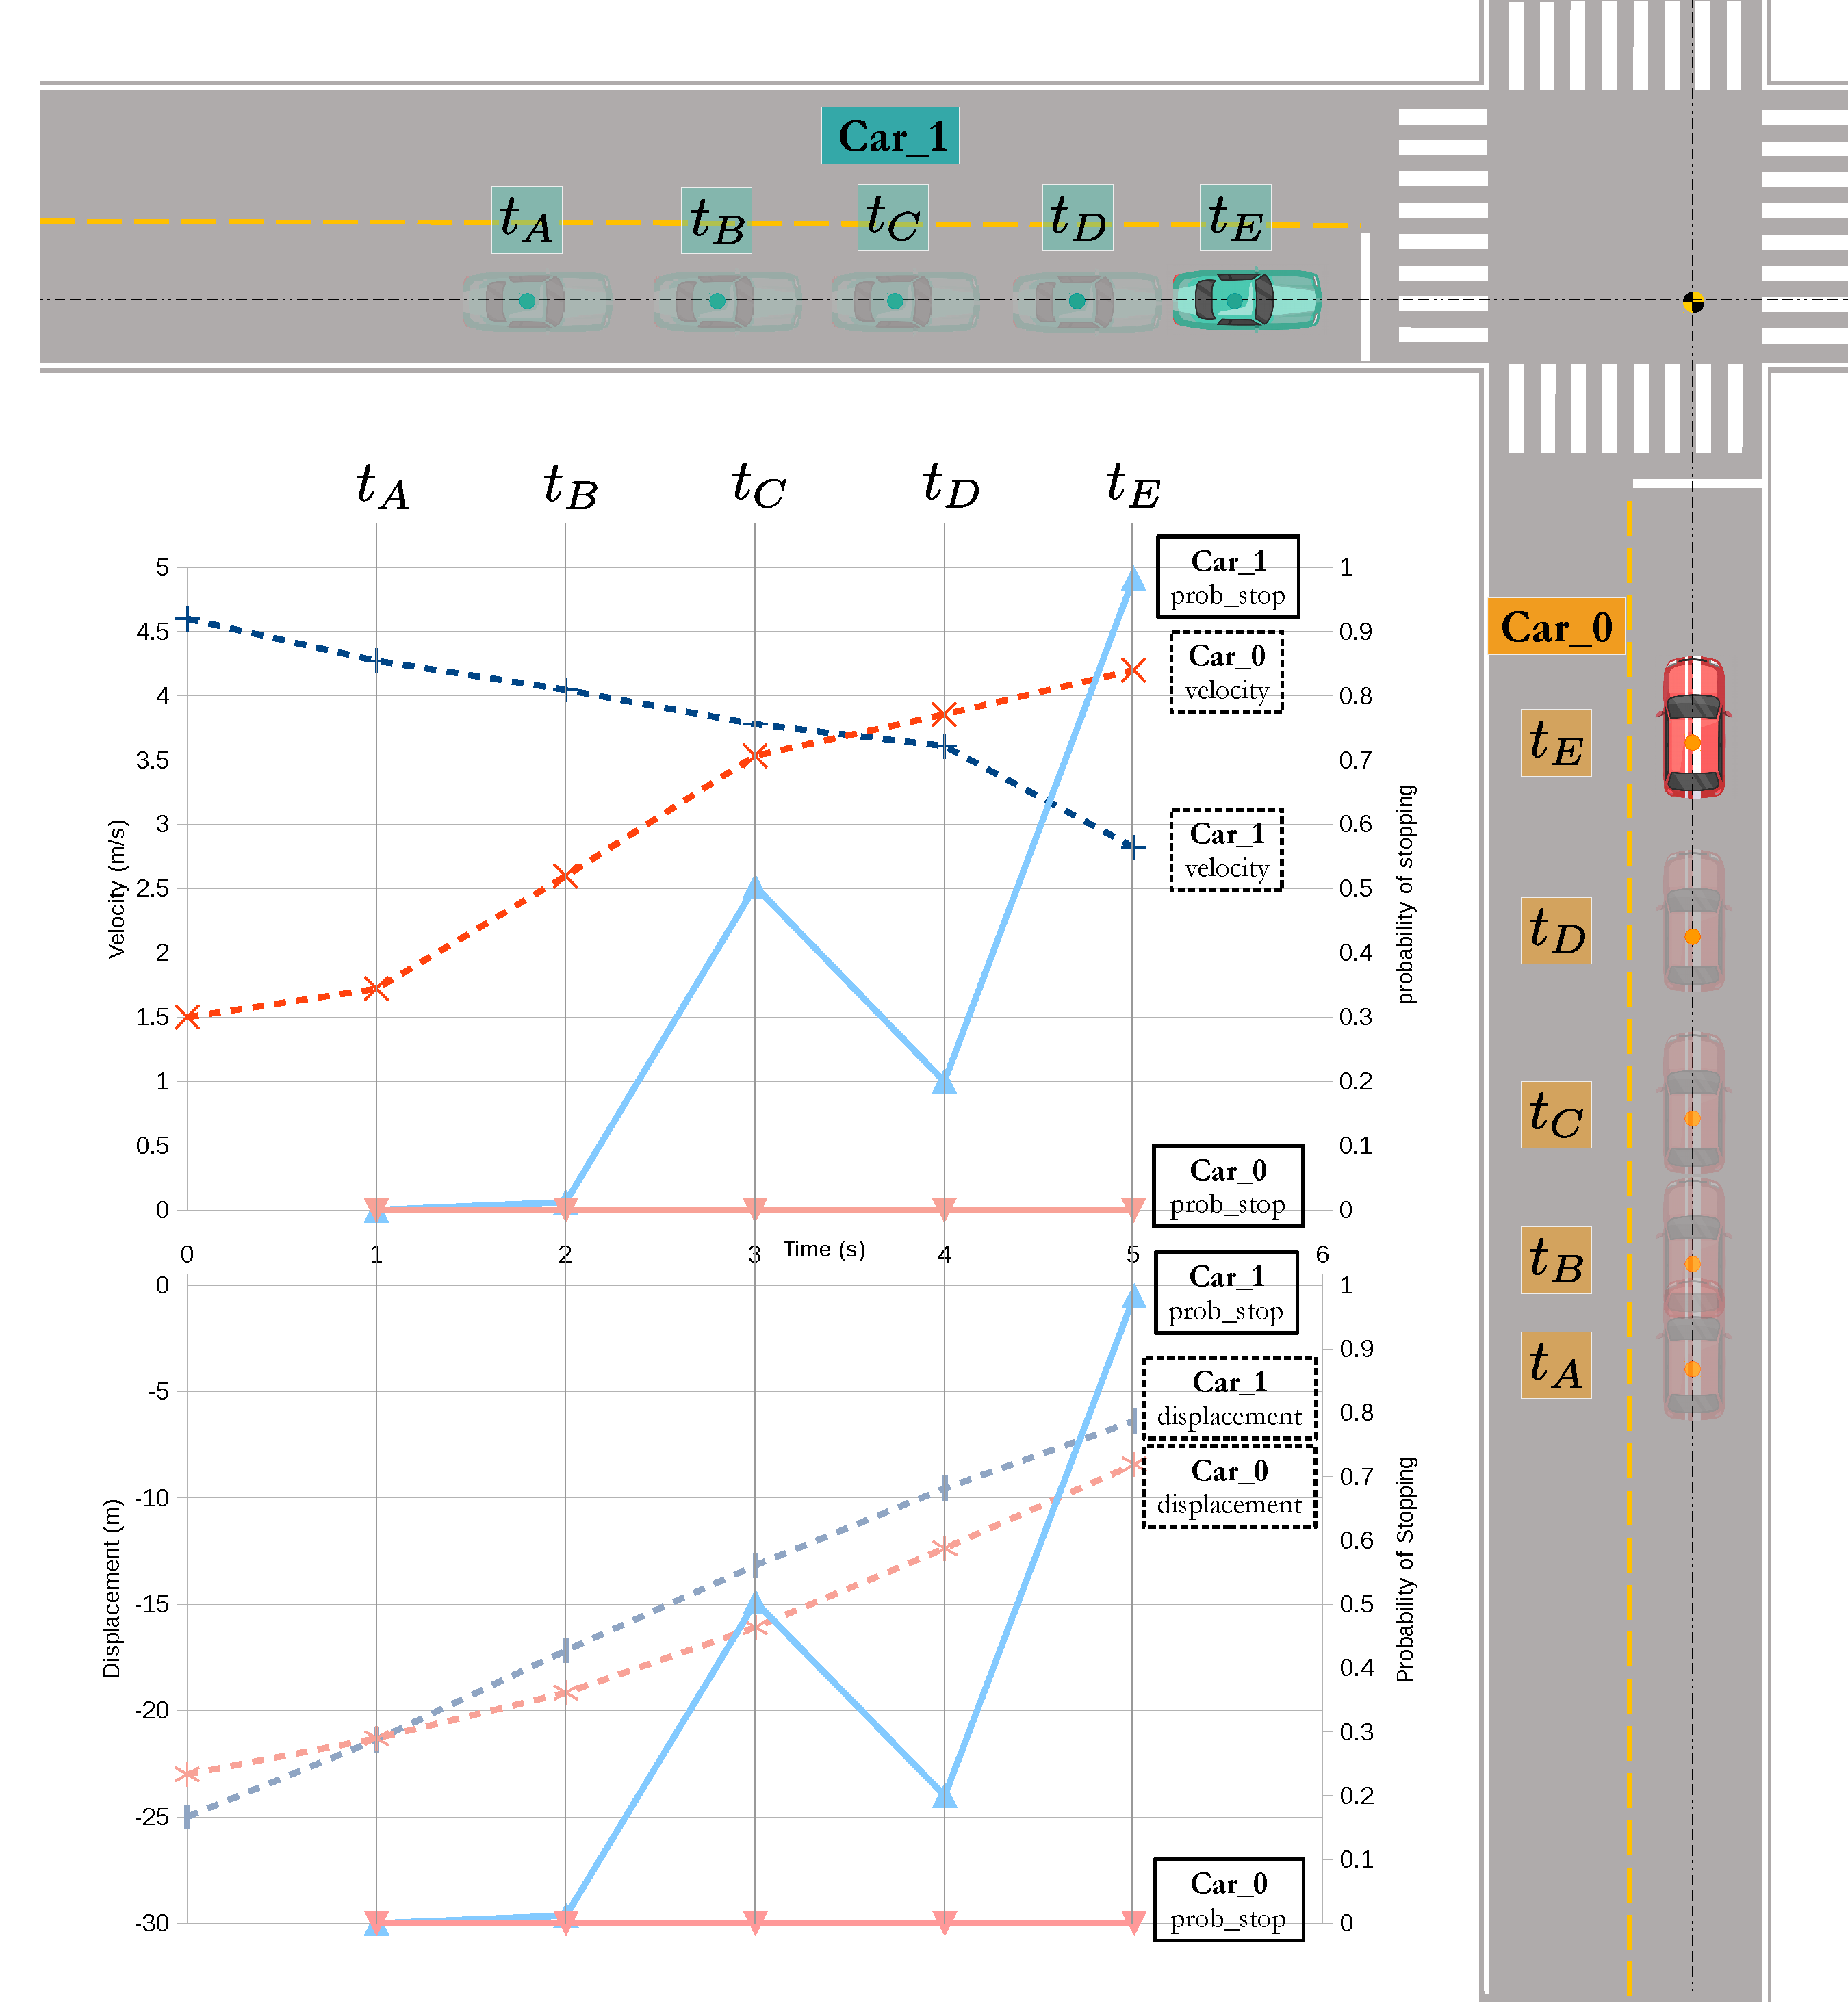
\includegraphics[width=0.47\textwidth]{figure_explaination_1.pdf}
    \label{fig:figure_explaination_1}
    }\hfill
    
    \caption{Illustration of TTC and probability of stopping along with concerning variables.} \label{fig:illustration}
\end{figure}

We start the analysis by calculating the corresponding TTC of Car\_0 (in red) and Car\_1 (in cyan), as illustrated in Fig.~\ref{fig:figure_explaination_TTC}. TTCs correspond to $t_A$, $t_B$, $t_C$, $t_D$ and $t_E$ are shown in the chart of the figure. Afterward, the probability of stopping for each car is calculated using the proposed method and is plotted together with the velocity and the displacement in two separate figures, as illustrated in Fig.~\ref{fig:figure_explaination_1}. The data collection begins when both of the displacements to the node is smaller than 18 meters where drivers are able to see each other, and ends when the node is reached by one of the participants. We then analyze how the probability of stopping can give assistance to the traffic participants using these figures.


Next, some of the experiments results will be presented to evaluate the performance of the proposed model. There will also be further explanations about the importance of parameters in the model. In the experiment conducted, trials are labeled with number (e.g. \#001, \#002, ...). The first interaction observed is trial \#003. 

\begin{figure}[htbp!]
\begin{center}
\makebox[0pt]{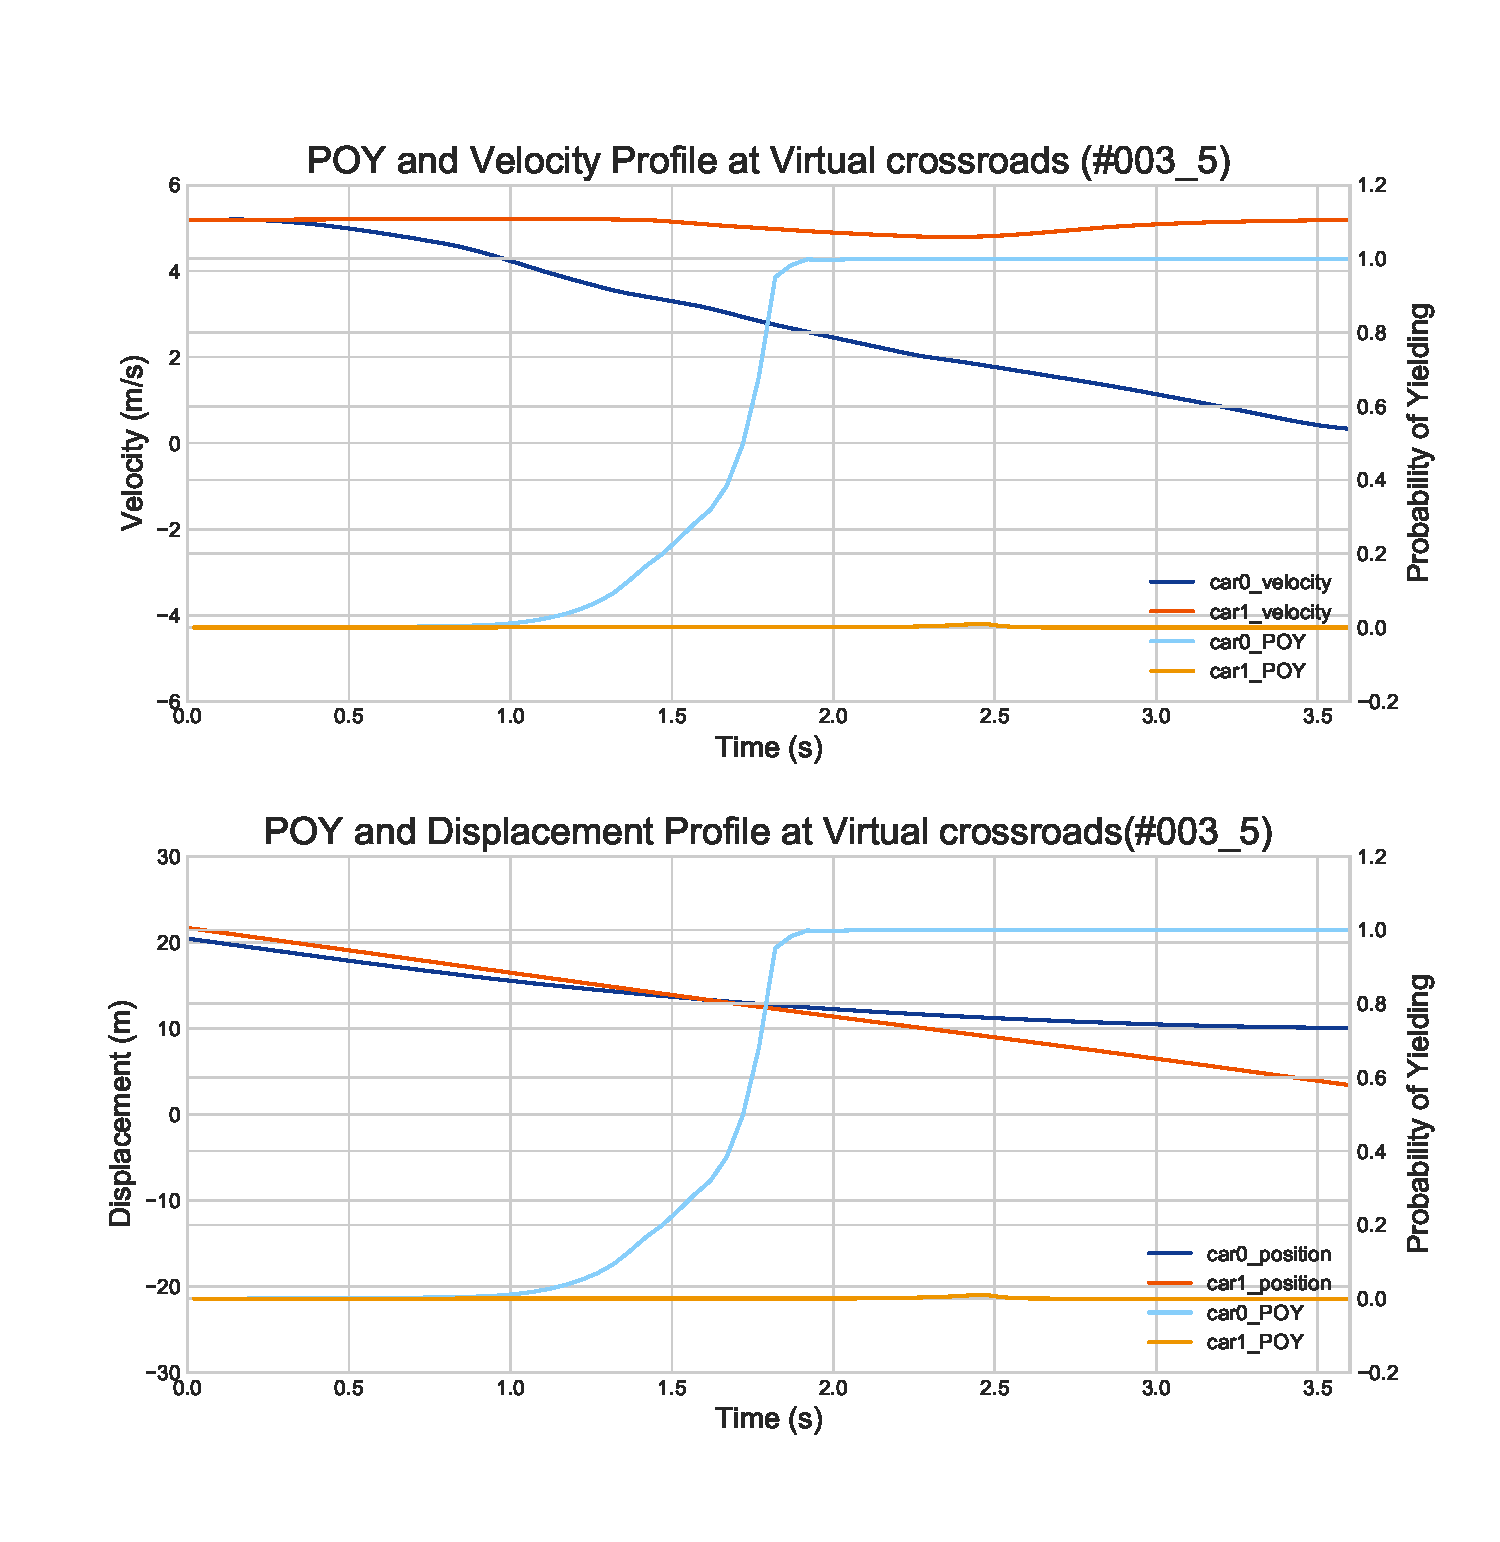
\includegraphics[width=0.65\paperwidth]{trial_003.pdf}}
\end{center}
\caption{Trial \#003 where car\_0 was yielding and car\_1 was passing with little interaction.}
\label{fig:trial003} 
\end{figure}

In this case, both yielding and passing types of drivers were included in this scene. Yielding type of drivers are those who will stop relatively early before the node, and slowly approach the intersection. They would only pass when the other agent is yielding. The passing type is the opposite, where there will be almost zero braking applied during the whole process. 


As presented in Fig.~\ref{fig:trial003}, driver of car\_0 was the yielding type because the deceleration started as soon as they could see each other in the sight (displacement at around 15 to 18 meters), and the driver of car\_1 was the passing type. During 0.8 to 1.8 sec, the POY of car\_0 was rising mainly due to the decreasing of the TTC at the moment, which was becoming smaller than the $TTA_{est}$ and resulted in more and more areas were under the TFA distribution and right to the TTC. The small spike on the POY curve of car\_1 around 2.5 was owing to the braking applied at about the same moment. In the next but one figure, this little bump will be elaborated. In this figure, the outcome suggests that the proposed model can correctly estimate the intention of the driver on other moving vehicles about 2 secs earlier.


\newpage


\begin{figure}[htbp!]
\begin{center}
\makebox[0pt]{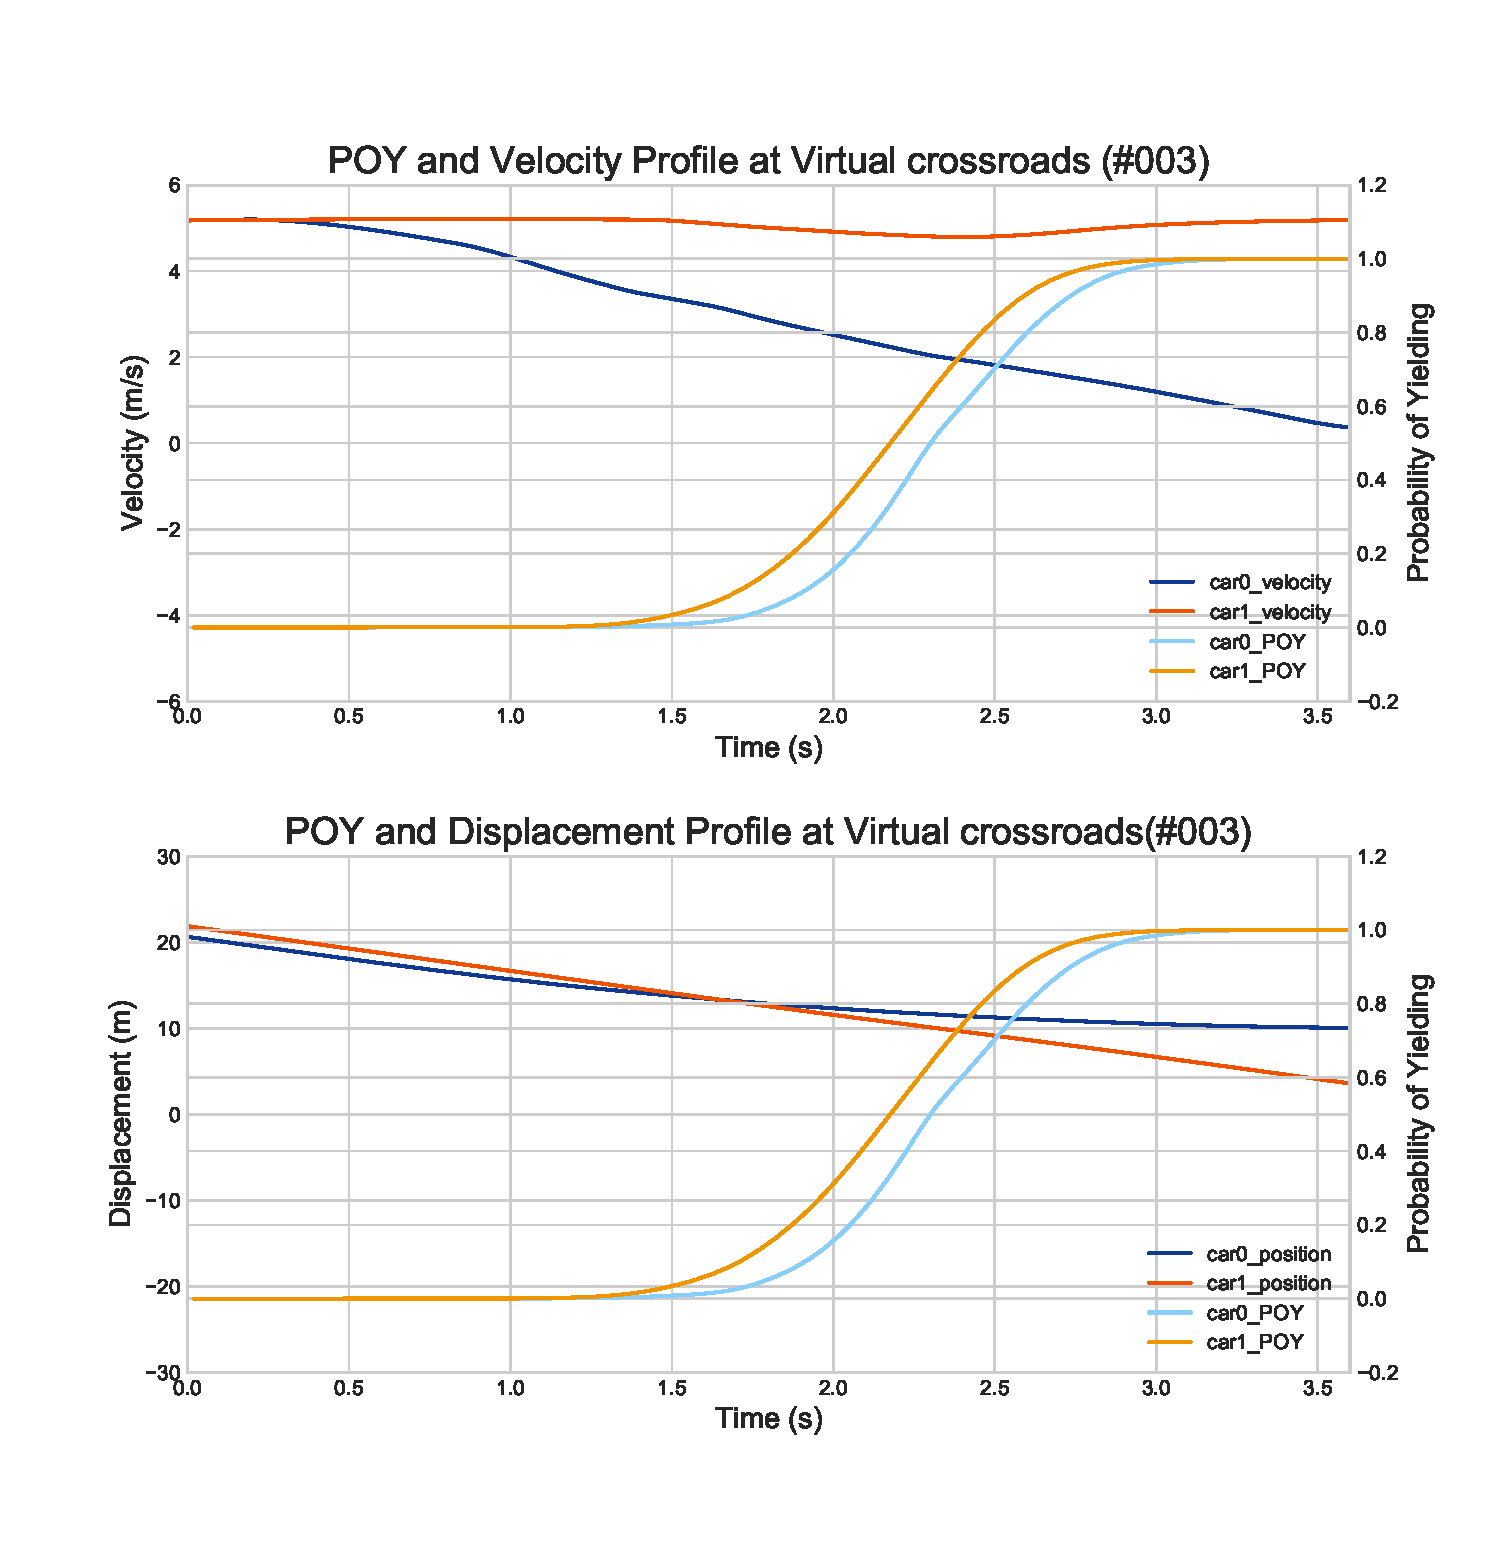
\includegraphics[width=0.65\paperwidth]{trial_003_WOalpha.pdf}}
\end{center}
\caption{Trial \#003 using POY without weighting parameter $A$ ($\alpha$).}
\label{fig:trial003WOalpha} 
\end{figure}



To demonstrate the importance of the weighting parameter $A$ ($\alpha$), which was formulated in Chapter \ref{chap:DriverModel}, the same trial (trial \#003) was evaluated again using the proposed POY model, but without the parameter $A$ ($\alpha$). Results are shown in Fig.~\ref{fig:trial003WOalpha}. Note that the POY of both vehicles rose to 1.0 from 1 to 3 sec. The main factor in this scenario was the displacement to the node which affected the $TFA_{est}$ and the $min TTC$. The plot showed that the closer the vehicle to the node, the higher the POY will be if it only depends on the displacement. Without the parameter $A$ ($\alpha$) being able to account for the acceleration and velocity and provide adjustments accordingly, the POY is unable to predict accurately. 

The conditions in Eqn.~\ref{eq:alpha} were also proved to be indispensable for the proposed model to produce a stable result in Fig.~\ref{fig:trial003WOcondition}. The huge spike occurred on the curve of car\_1 POY around 1.2 to 2.5 secs was the consequence of the proposed model being too "sensitive" about some small changes in acceleration that usually do not imply the intention to yield. Constraints such as the maximum deviation for the TFA distribution (as formulated in Eqn.~\ref{eq:alpha_cap}) or the threshold for acceleration longer than 0.2 sec are employed to prevent the POY from being too sensitive to accelerations.

\begin{figure}[htbp!]
\begin{center}
\makebox[0pt]{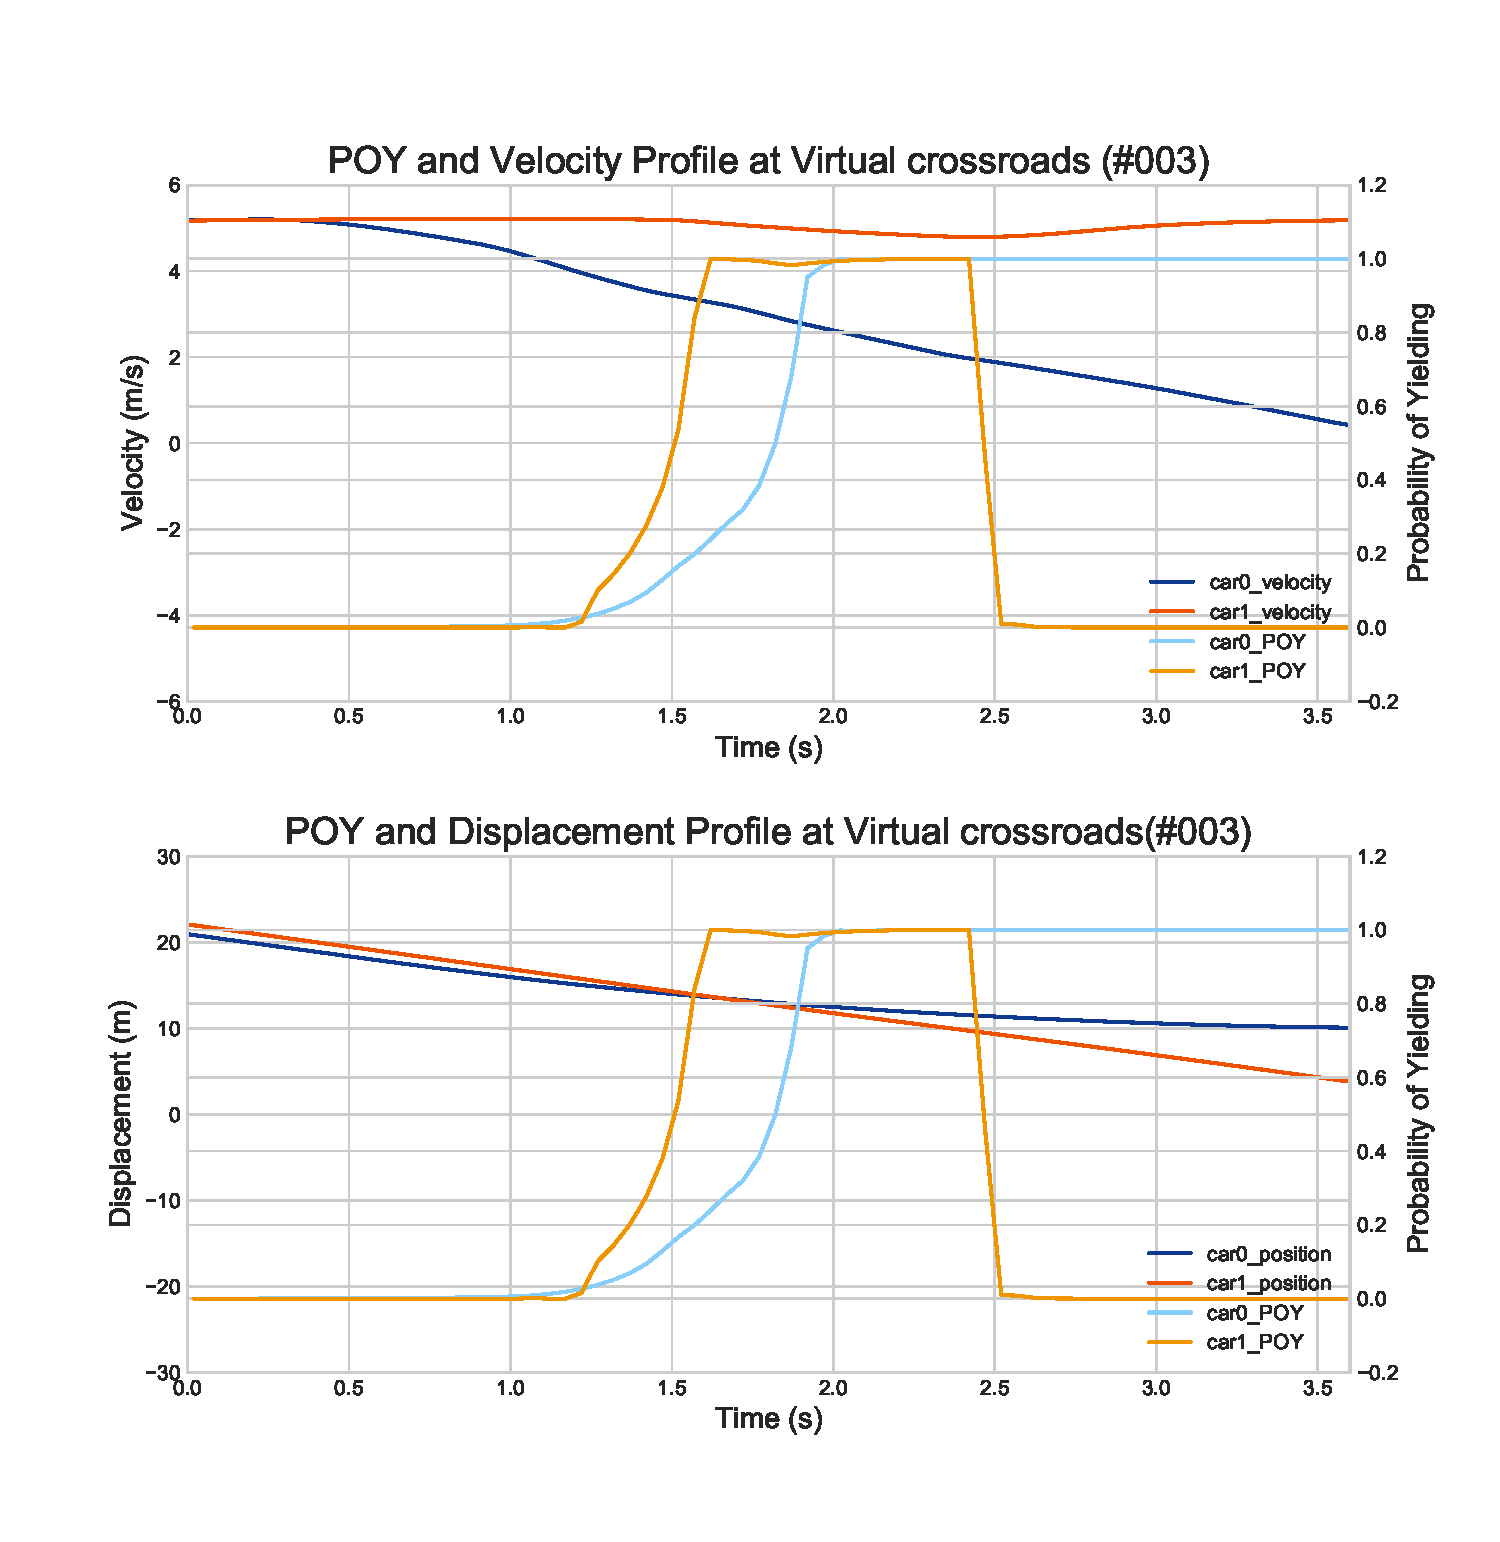
\includegraphics[width=0.65\paperwidth]{trial_003_WOcondition.pdf}}
\end{center}
\caption{Trial \#003 using POY without acceleration threshold.}
\label{fig:trial003WOcondition} 
\end{figure}


The second case of interaction is more interactive than trial \#003. In trial \#077, both drivers were indecisive, since both participants were quite even at their states and no one was in dominant position. In the most extreme cases, it will take both drivers quite a long time before one of them decides to pass or yield. In trial \#077, however, it did not take them too long before car\_0 finally decide to pass. At the beginning of the interaction, POYs of both vehicles rose due to their deceleration. And from 1.5 to 3.2 secs, the POYs were kept at high level for car\_0, while car\_1 had the intention to pass, which resulted in the drop of POY. But right after car\_1 accelerated, so did car\_0 with very small time difference (0.5 sec). And after about a second, they both decelerated together again, but this time car\_1 was determined to yield and car\_0 finally passed. During this time, human drivers had no information about what actions the other one intended to take, so they waited until one of them did something. Yet, if one could utilize the proposed model which could estimate the TFA distribution of the driver and generate a probability from his or her current states, this stnad-off-like situation could have been avoided. 

\begin{figure}[htbp!]
\begin{center}
\makebox[0pt]{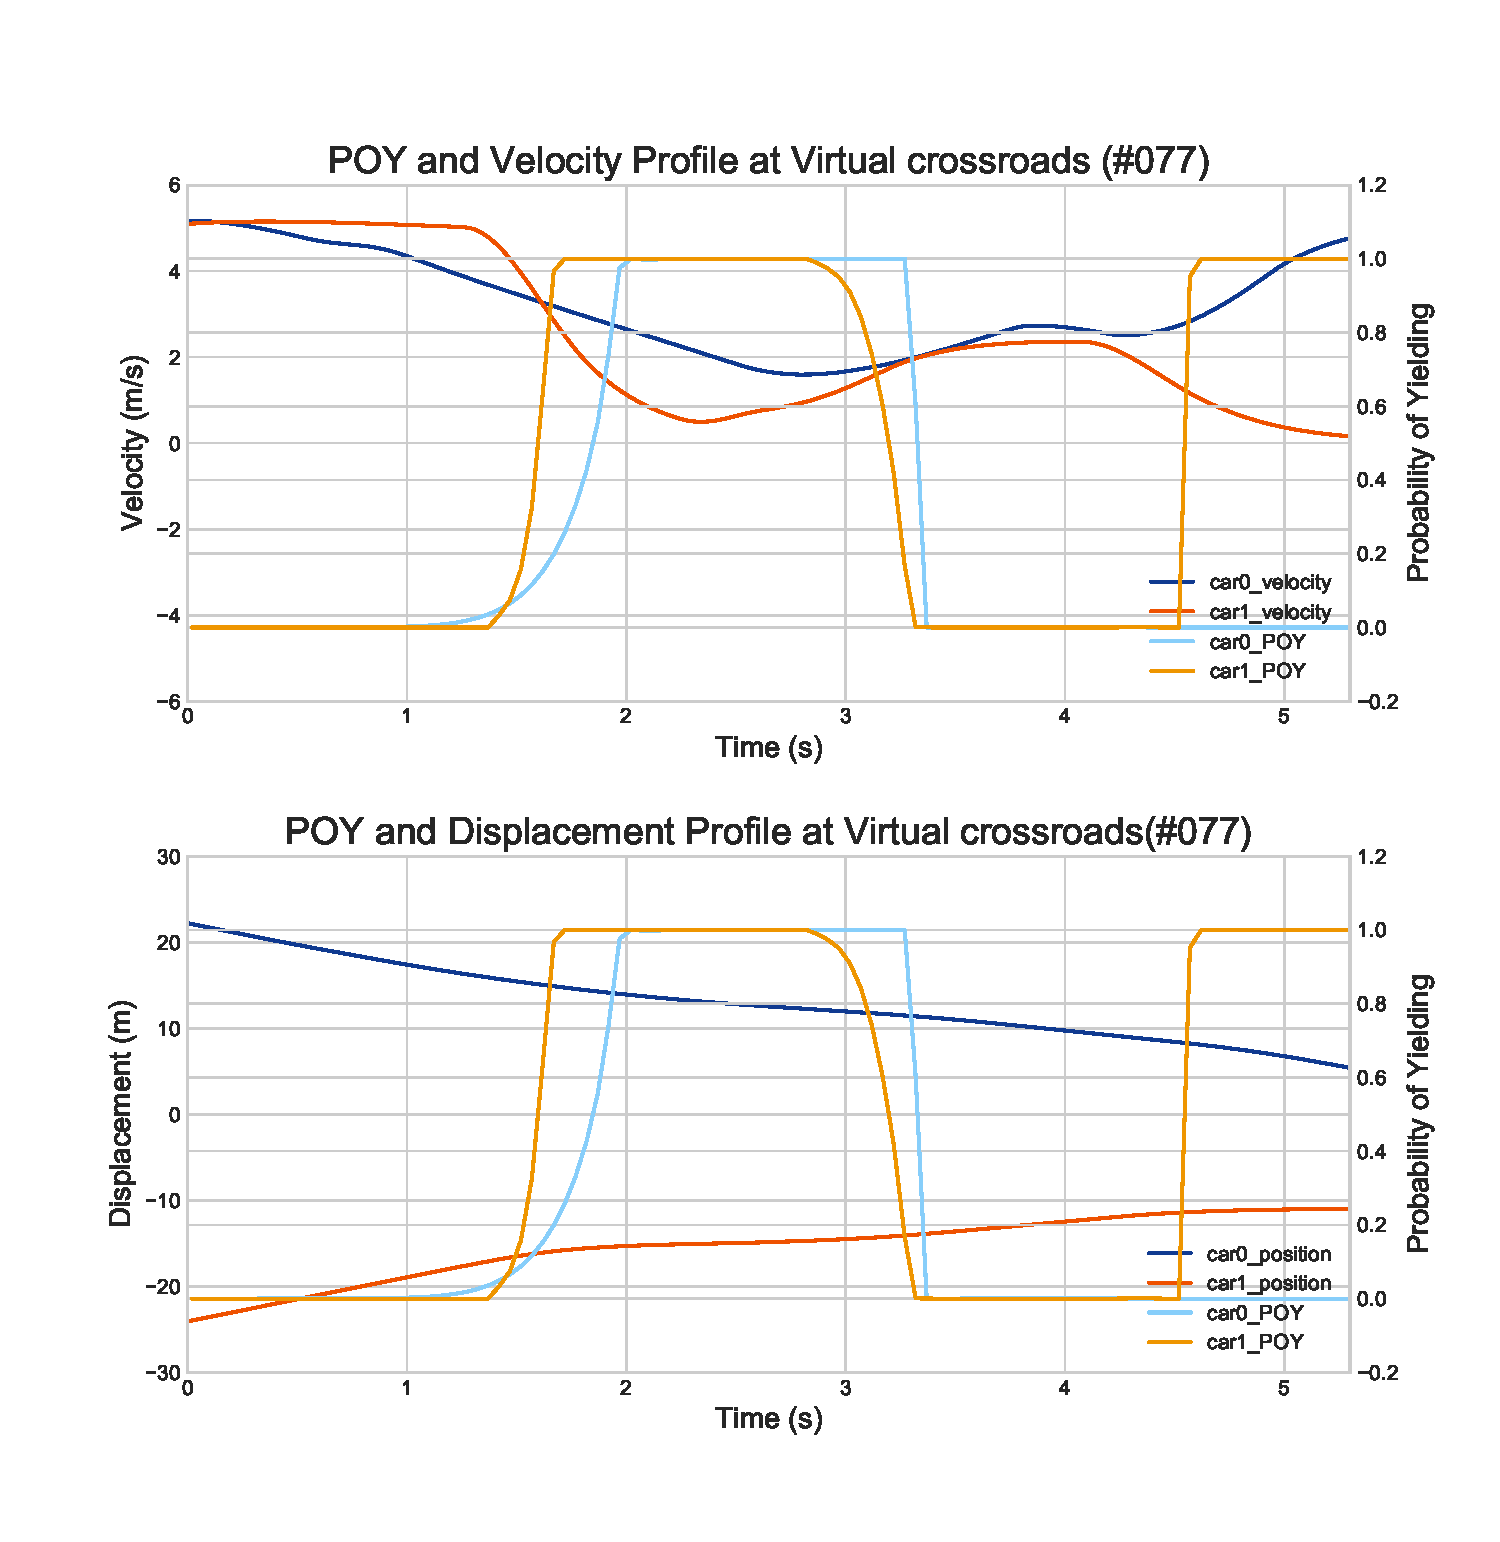
\includegraphics[width=0.65\paperwidth]{trial_077_indecisive.pdf}}
\end{center}
\caption{Trial \#077 where car\_0 and car\_1 were confused about what action the other one might take.}
\label{fig:trial077} 
\end{figure}


The final case presented can again show how one can benefit from the proposed model. In Fig.~\ref{fig:trial063}, car\_0 was a bit closer to the node and it yielded to let car\_1, who was farther but had no intention to yield, passed first. However, car\_1 did not think that the deceleration of car\_0 was intended to yield, so it chose to yield too and car\_0 then accelerated to pass. Again, this situation could have been avoided if the proposed method is referenced by the driver.


\begin{figure}[htbp!]
\begin{center}
\makebox[0pt]{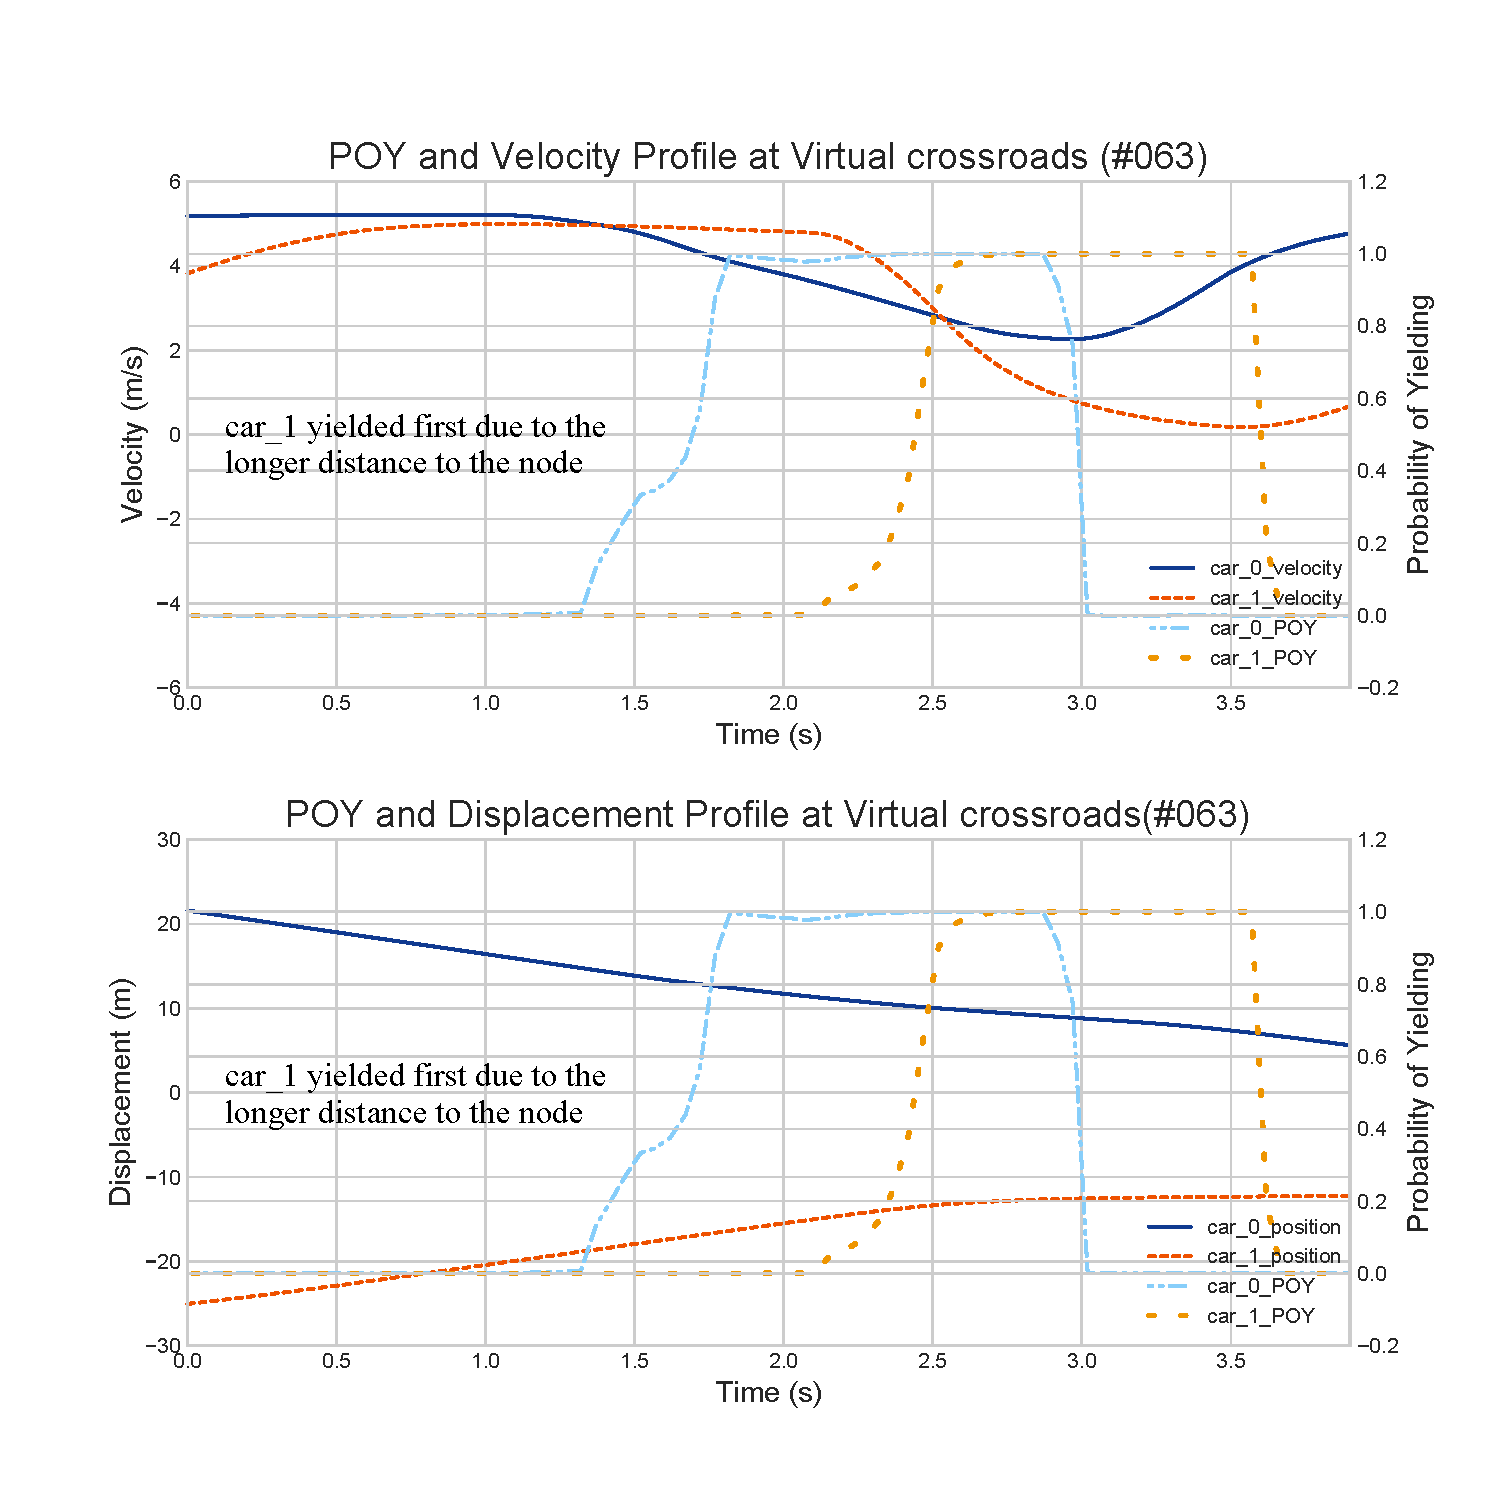
\includegraphics[width=0.65\paperwidth]{trial_063_bothyield.pdf}}
\end{center}
\caption{Trial \#063 where car\_0 yielded first but then passed due to the deceleration of car\_1 .}
\label{fig:trial063} 
\end{figure}

\newpage

%%%%%%%%------------------------------%%%%%%%%%
%%%%%%%%-----------SUBSECTION---------%%%%%%%%%
%%%%%%%%------------------------------%%%%%%%%%
\subsection{Validation for Experiments in Simulated Environment}
\label{sub:ValidationSim}


In Section \ref{sub:ResultSim}, the proposed model is proved to be comparable to human drivers' prediction and the decisions of human drivers are managed to turn into some probabilistic values, which can be perceived by autonomous vehicles. In this section, the accuracy of the proposed model will be examined.

\begin{equation}
    CARate = \frac{\text{number of correctly classified situations}}{\text{number of all situations}}
\label{eq:CARate}
\end{equation}

The \ac{CARate} is used to evaluate the calssification accuracy of the proposed model. Due to the fact that the time spans for all interaction trials are different, the time line is be reversed and denoted as $T_{minus}$, i.e., $T_{minus}=0$ denotes the time at the end of the process and $T_{minus}=1$ denotes the time 1 sec earlier than that, and so on. Note that the end of the process is defined as the moment which the node is reached by one of the participants. The calculation of CARate is rather straight forward as shown in Eqn.~\ref{eq:CARate}. In the total of 168 cases of driver behaviors at the crossroad, the denominator of the CARate at each $T_{minus}$ is then 168. The CARate results of the proposed model are shown in Fig.~\ref{fig:CARPOY}.

\begin{figure}[htbp!]
\begin{center}
\makebox[0pt]{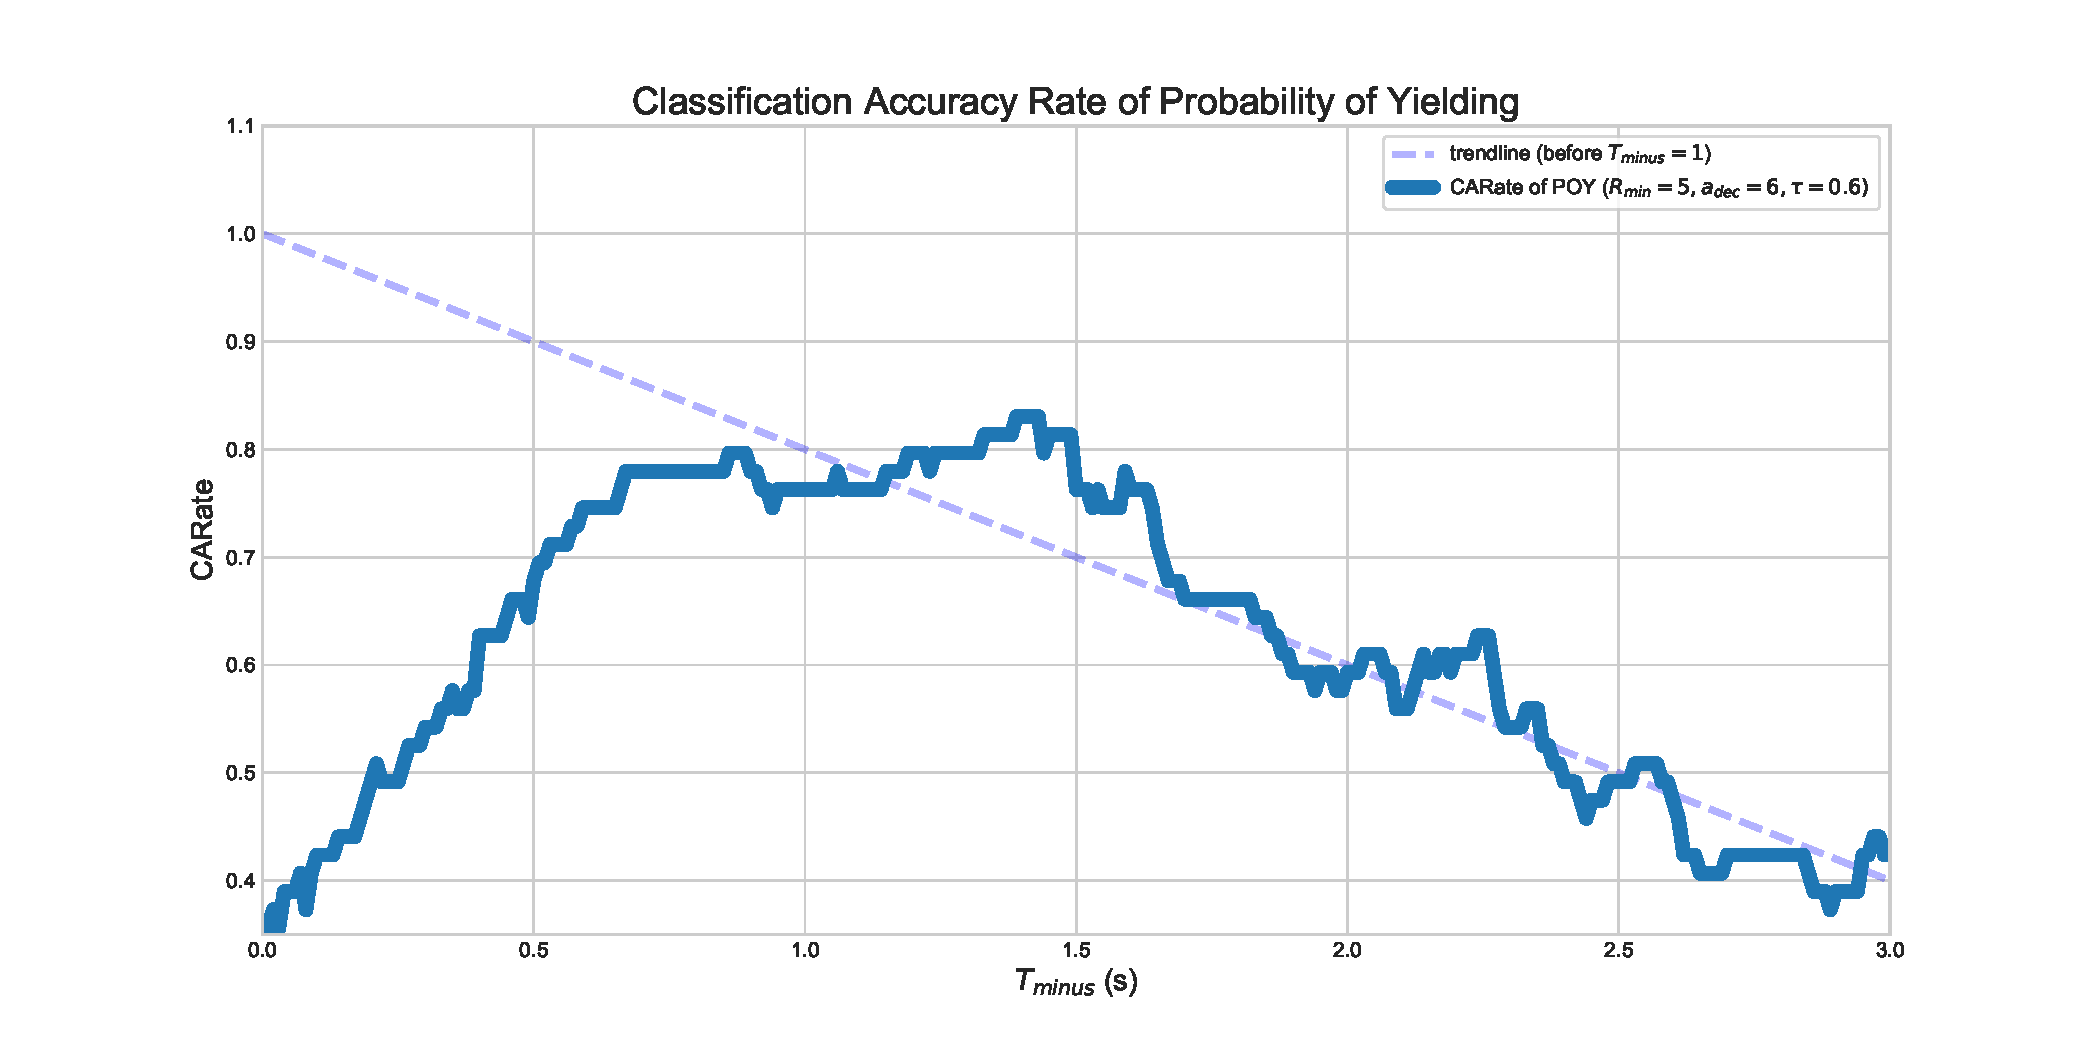
\includegraphics[width=0.72\paperwidth]{CARPOY.pdf}}
\end{center}
\caption{CARate of the POY using all data sets.}
\label{fig:CARPOY} 
\end{figure}

Results using the average parameters listed in Table.~\ref{table:parameters} are plotted in solid blue line while the trend line is plotted in dashed blue line. The reason for the drop from 0.0 to 1.5 $T_{minus}$ is that, people tend to behave more aggressive in our simulated environments. During the experiment, participants who yielded for the other driver accelerated before the end of the process which is the moment when the node is reached. The example is shown in Fig.~\ref{fig:trial039}.

\begin{figure}[htbp!]
\begin{center}
\makebox[0pt]{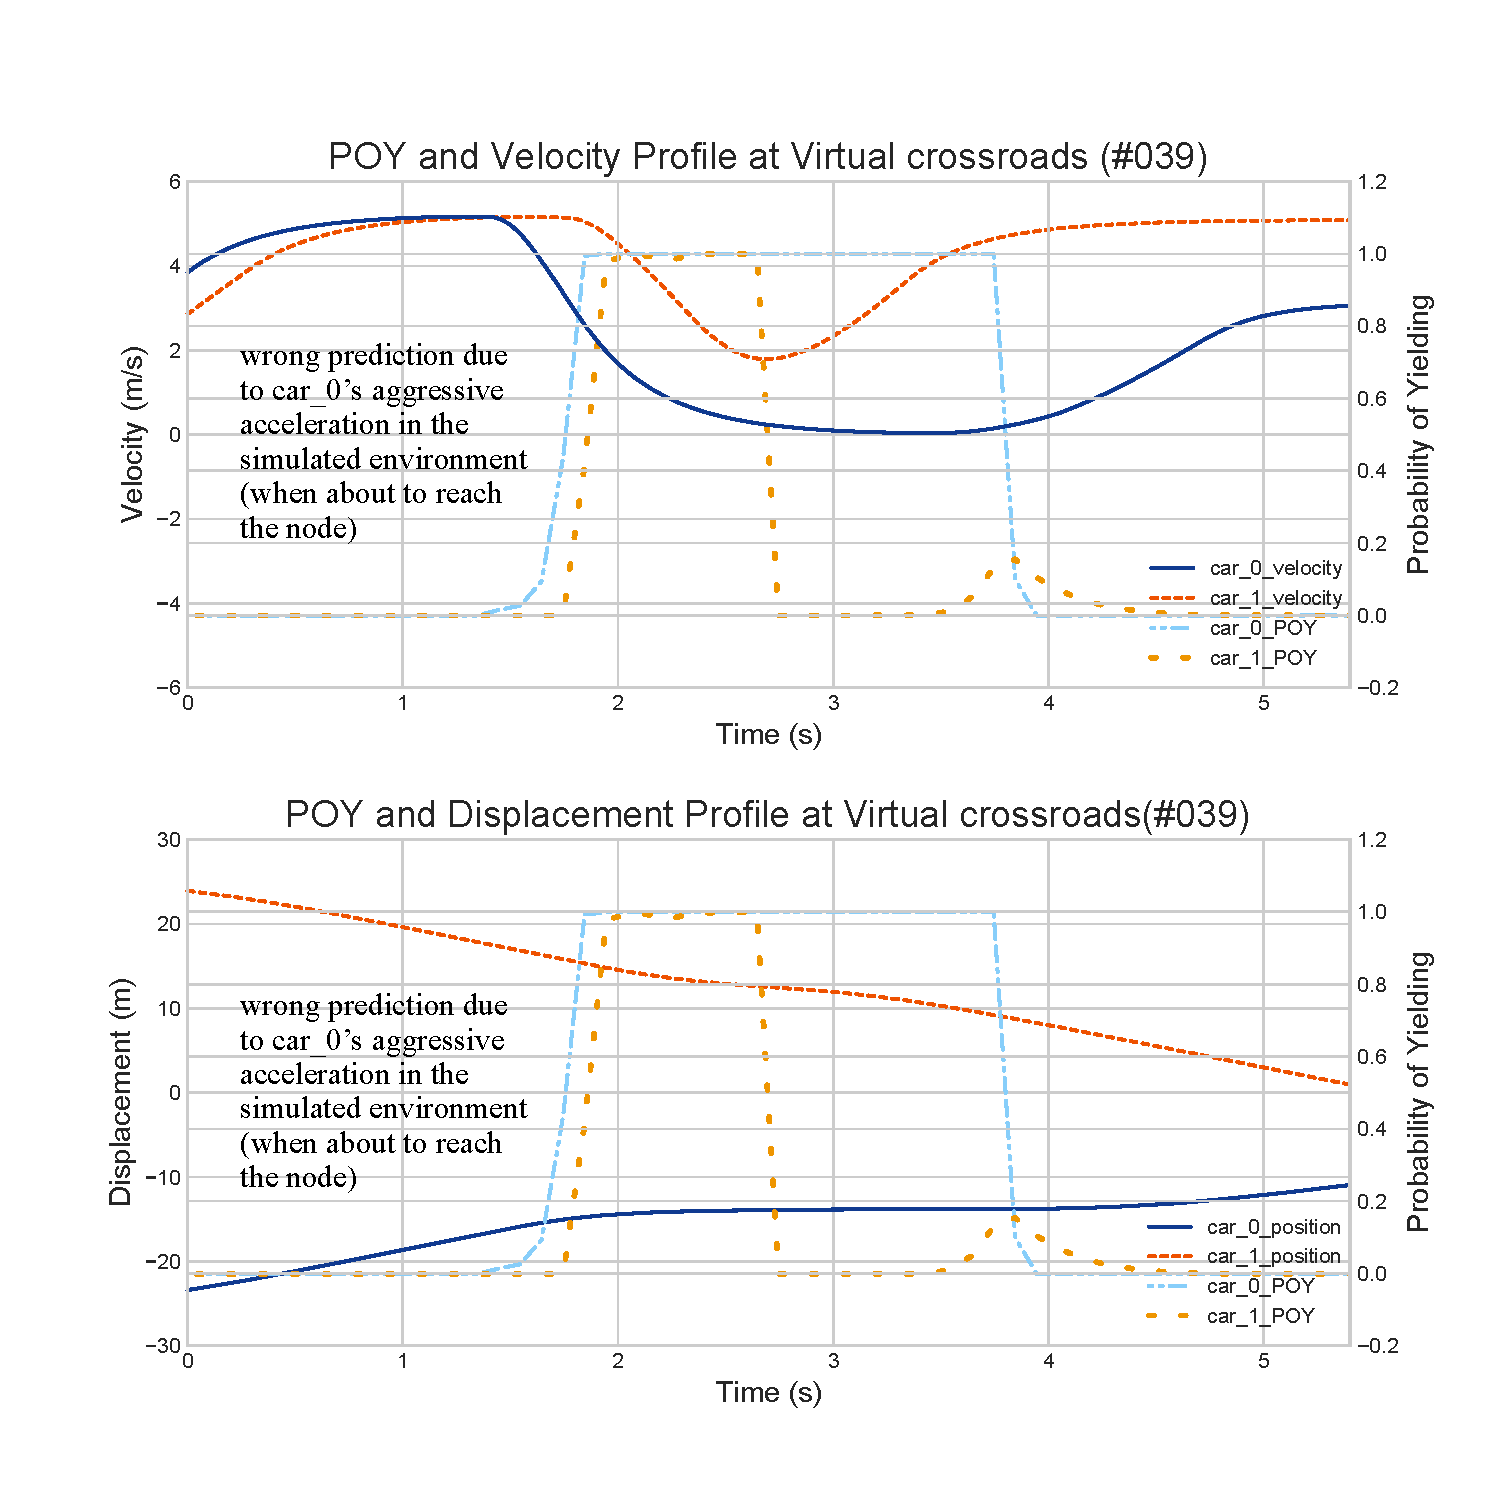
\includegraphics[width=0.65\paperwidth]{trial_039_toosoon.pdf}}
\end{center}
\caption{Trial \#039 where car\_1 begun to accelerate before car\_0 passed the node, causing the false prediction.}
\label{fig:trial039} 
\end{figure}

Comparing to other few behavior prediction model, the CARate of the proposed model is comparable to the state-of-the-art. In the work of Graf et al. \cite{Graf2014}, the CARate reached 0.81 at around $T_{minus} = 3$, while in the proposed model 0.81 is reached at $T_{minus} = 1.5$. This is owing to the relatively short interaction time span in the simulated environment, where participants are using joysticks sending out maximum command velocity. In the literature, interactions at real crossroads takes about 6 secs to cross a 12 to 18 meters long distance, yet at the simulated crossroad, it only takes about 3.5 secs to cross 20 meters. Furthermore, the method proposed in the literature requires pre-trained model for a specific where in POY no training steps are needed. The proposed POY also has the potential of generating better predictions if the parameters characterizing his or her driving pattern is known.


In this chapter, a novel driver behaviors model at crossroads was proposed. Driver intentions were predicted based on the parameter TTC, which is an important and well developed risk estimation method in traffic safety assessment. Derived form the concept, the TFA distribution was shown to be an innovative and effective driver intentions indicator that can be used to predict the driver behaviors. The normally distributed TFA distribution was then formulated and proven to be an unerring approximation. At last the driver behaviors model was finally proposed and validated at the simulated crossroad where prediction accuracy was comparable to the state-of-the-art driver behaviors prediction method. 

\chapter{Model Parameters Identification}
\label{chap:ModelParam}
\resetfigpath{Chap4}

%%%{INTRODUCTION to this CHAPTER}%%%

In Chapter ~\ref{chap:DriverModel}, a model providing a probabilistic way to evaluate the possible behaviors of other traffic participants was proposed. The concept of the fact that TFA distributions are different among people was also elaborated and formulated in Eqn.~\ref{eq:TFA_est}. Then, the average parameter of participants were found and used to estimate the POY in the experiment at the simulated crossroad. In this chapter, the characteristic parameters of drivers will be attempted to identify.


%%%%%%%%%%%%%%%%%%%%%%%%%%%%%%%%%%%%%%%%%%%%%%%%%%%%%%%%%%%%%%%%%%%%%%%%
%%%%%%%%%%               SECTION SECTION SECTION               %%%%%%%%%
%%%%%%%%%%%%%%%%%%%%%%%%%%%%%%%%%%%%%%%%%%%%%%%%%%%%%%%%%%%%%%%%%%%%%%%%
\section{Characteristic Parameters}
\label{sec:characterParam}

The way people drive is different from person to person, some are aggressive, while others are more conservative. This also applies to the decision on braking moment. In Section ~\ref{sec:TFADistribution}, the mean value of TFA distribution of drivers is formulated in Eqn.~\ref{eq:TFA_est}, where three parameters including $R_{min}$ and $a_{dec}$ are introduced. The $R_{min}$, standing for the minimum distance left when the vehicle is fully stopped, being a parameter known as a function of velocity of the vehicle, is also changing with different characters. To put it another way, two different driver driving two identical vehicles under same speed would have different mean distance left before the vehicle and the obstacle when the vehicle stops moving. This is a rather instinctive results since a more aggressive people tend to brake as late as possible which contributes to the smaller $R_{min}$. Similarly, drivers who make traffic offense are having higher $a_{dec}$ than those more conservative.

What can be learned from Eqn.~\ref{eq:TFA_est} is that, each of these parameters can put effect on the value of ${TTA}_{est}$, in other words, they decide the value of ${TTA}_{est}$ and the results of POY. In Fig.~\ref{fig:trial003params} and Fig.~\ref{fig:trial077params}, the POY using the average parameters and the driver's parameters are compared. As we can see in these cases, the POYs of the vehicle (car\_0 in Fig.~\ref{fig:trial003}) are higher using the characteristic parameters belonging to the driver. 



\begin{figure}[htbp!]
\begin{center}
\makebox[0pt]{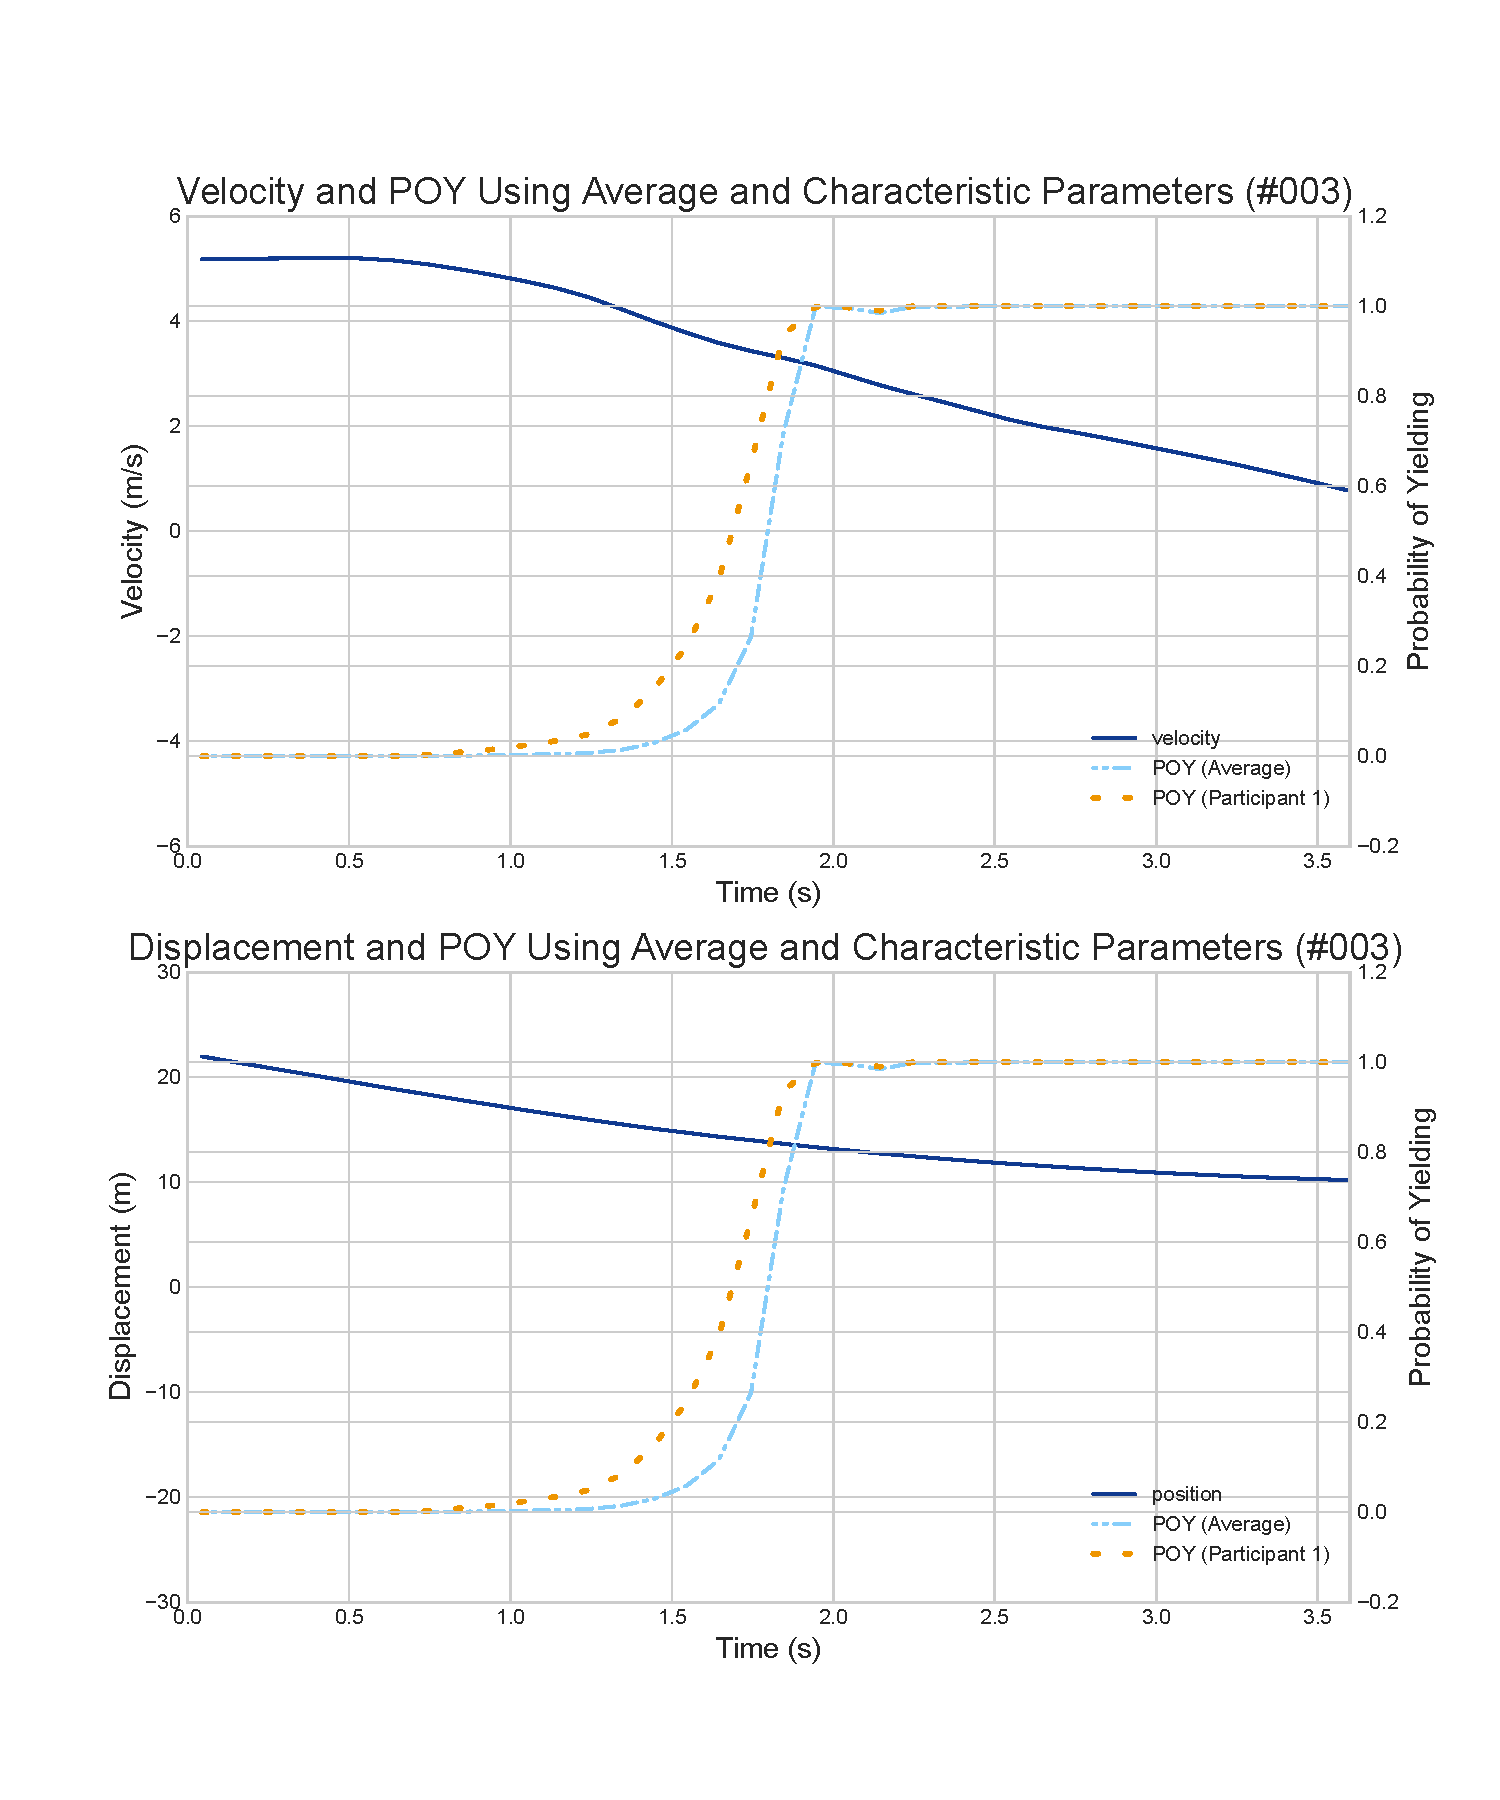
\includegraphics[width=0.65\paperwidth]{compare_trial_003.pdf}}
\end{center}
\caption{Trial \#003 with POY using average parameters and parameters of Participant 1.}
\label{fig:trial003params} 
\end{figure}

\begin{figure}[htbp!]
\begin{center}
\makebox[0pt]{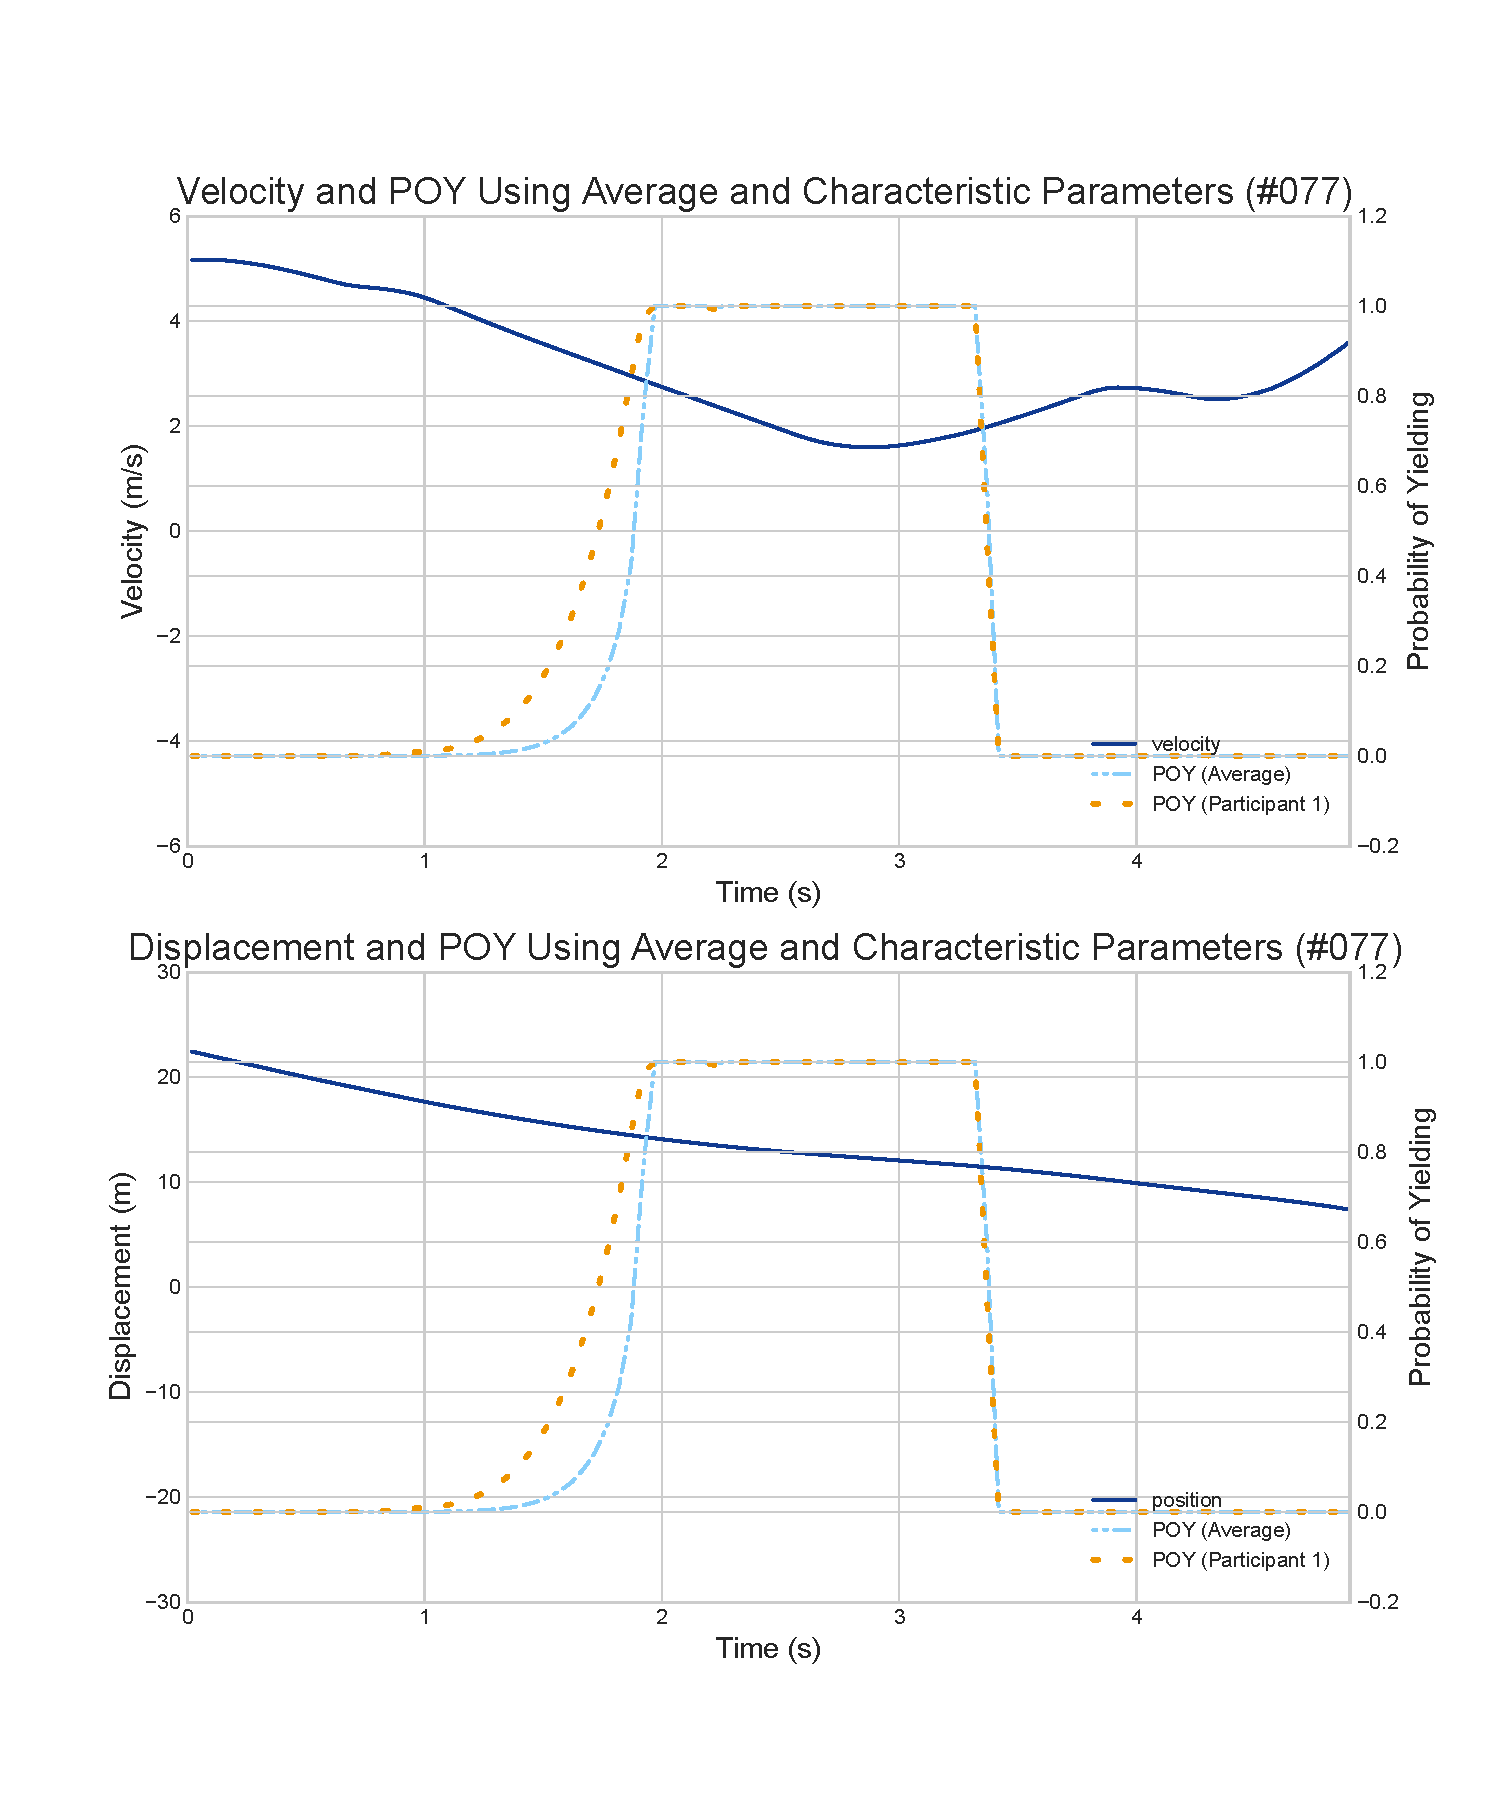
\includegraphics[width=0.65\paperwidth]{compare_trial_077.pdf}}
\end{center}
\caption{Trial \#077 with POY using average parameters and parameters of Participant 1.}
\label{fig:trial077params} 
\end{figure}


This phenomenon is owing to the closer estimation of the TFA distribution. Bringing a set of average parameters into Eqn.~\ref{eq:TFA_est} will only give an rough whereabouts of the TFA of the driver at the moment (considering velocity, displacement to the node and so on). Using the specific characteristic parameters, on the other hand, could effectively narrow down the TFA of the driver to within the consequential TFA distribution. Still, chances are that the estimated TFA distribution using the characteristic parameter might be different from the real TFA under the circumstance, given that both of them are distributions. However, given a large enough database, the average POY acquired using characteristic parameters should be higher than that using average parameter.


\begin{figure}[htbp!]
\begin{center}
\makebox[0pt]{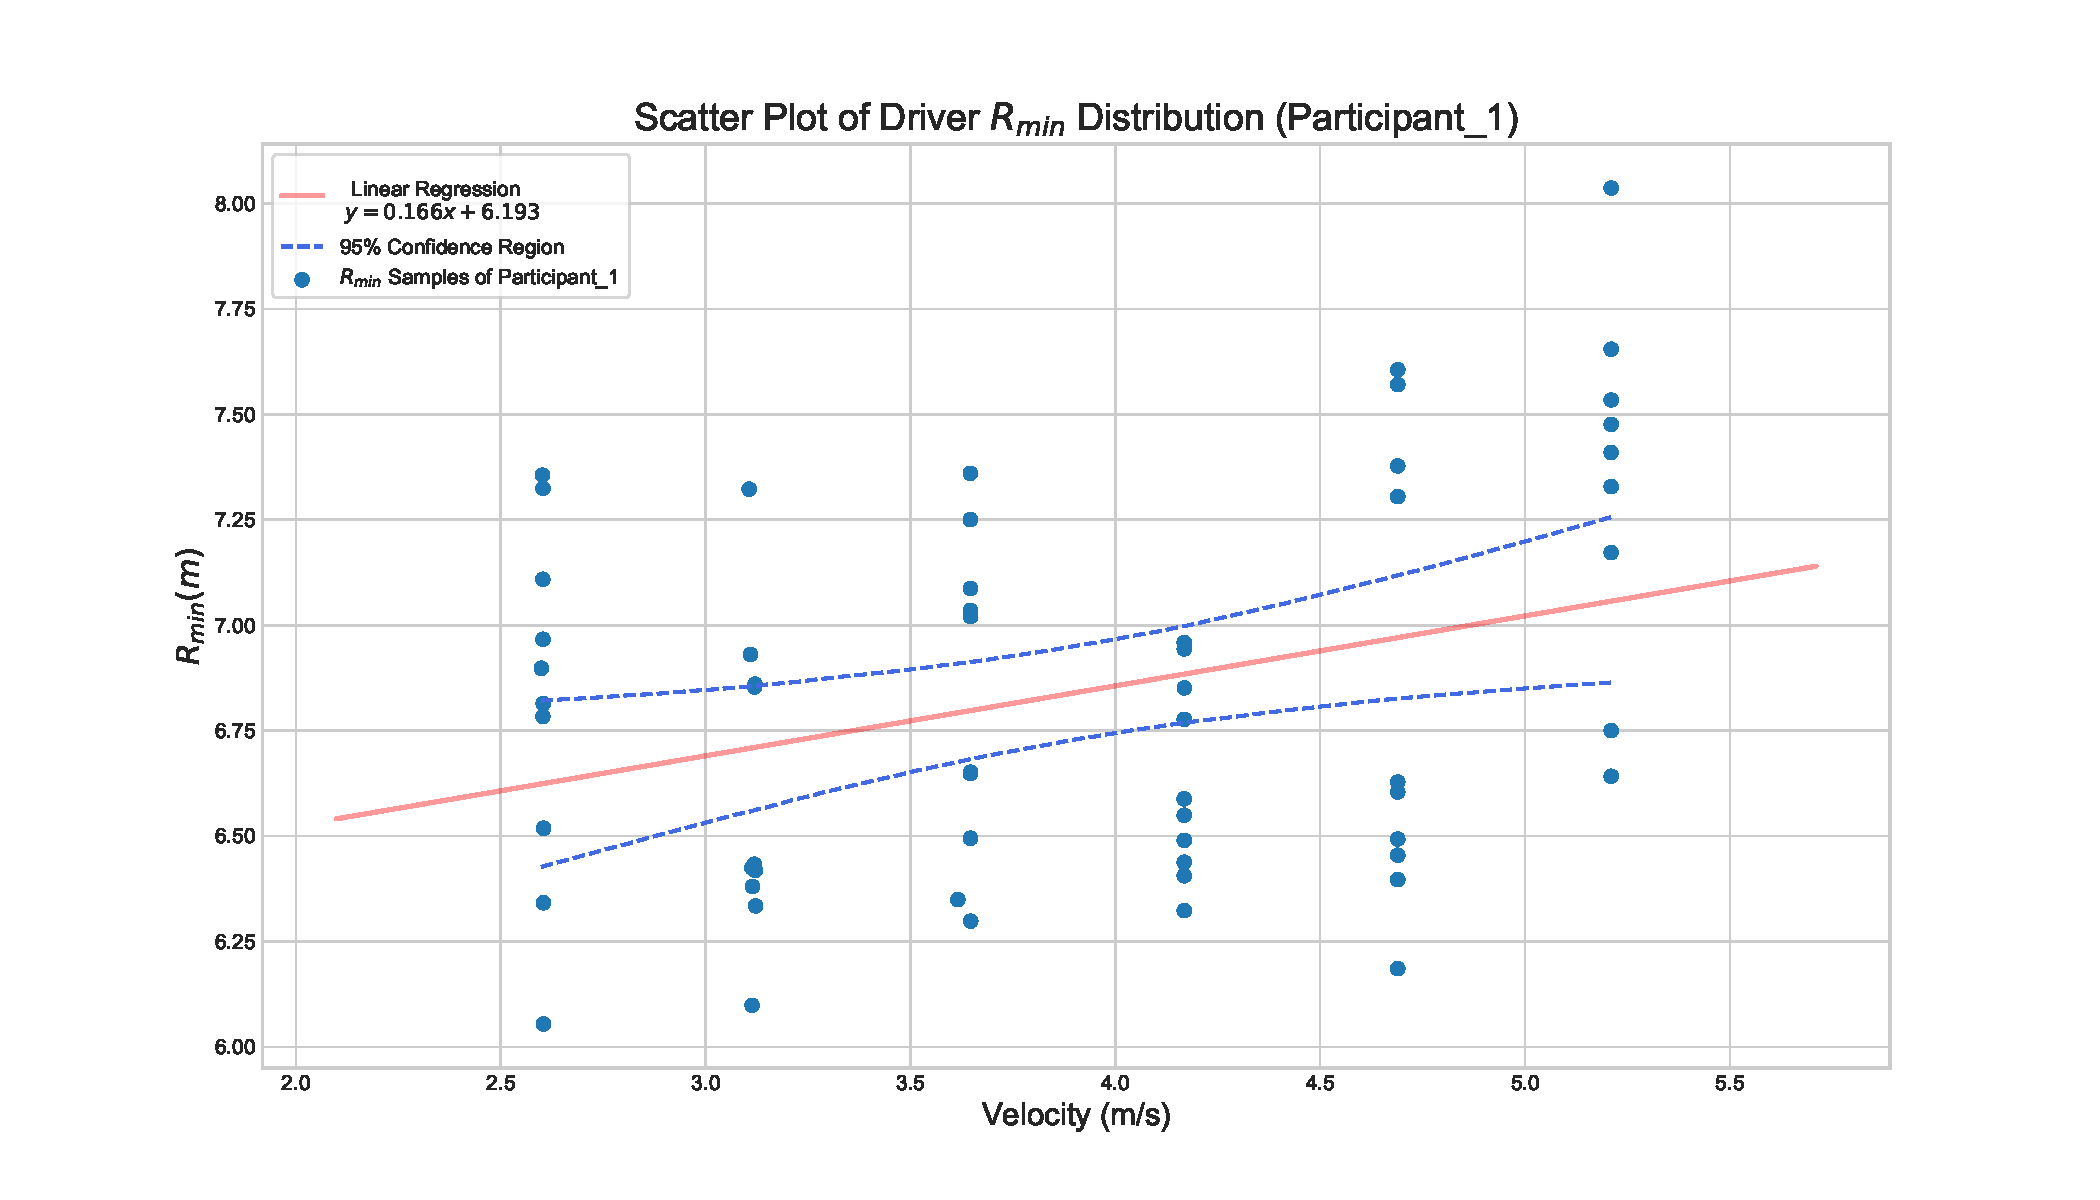
\includegraphics[width=0.7\paperwidth]{/Participant_1_R_MIN_polyfit.pdf}}
\end{center}
\caption{The $R_{min}$ scatter plot of Participant 1 under various velocities.}
\label{fig:Par1RMINDifSpeed} 
\end{figure}

\begin{figure}[htbp!]
\begin{center}
\makebox[0pt]{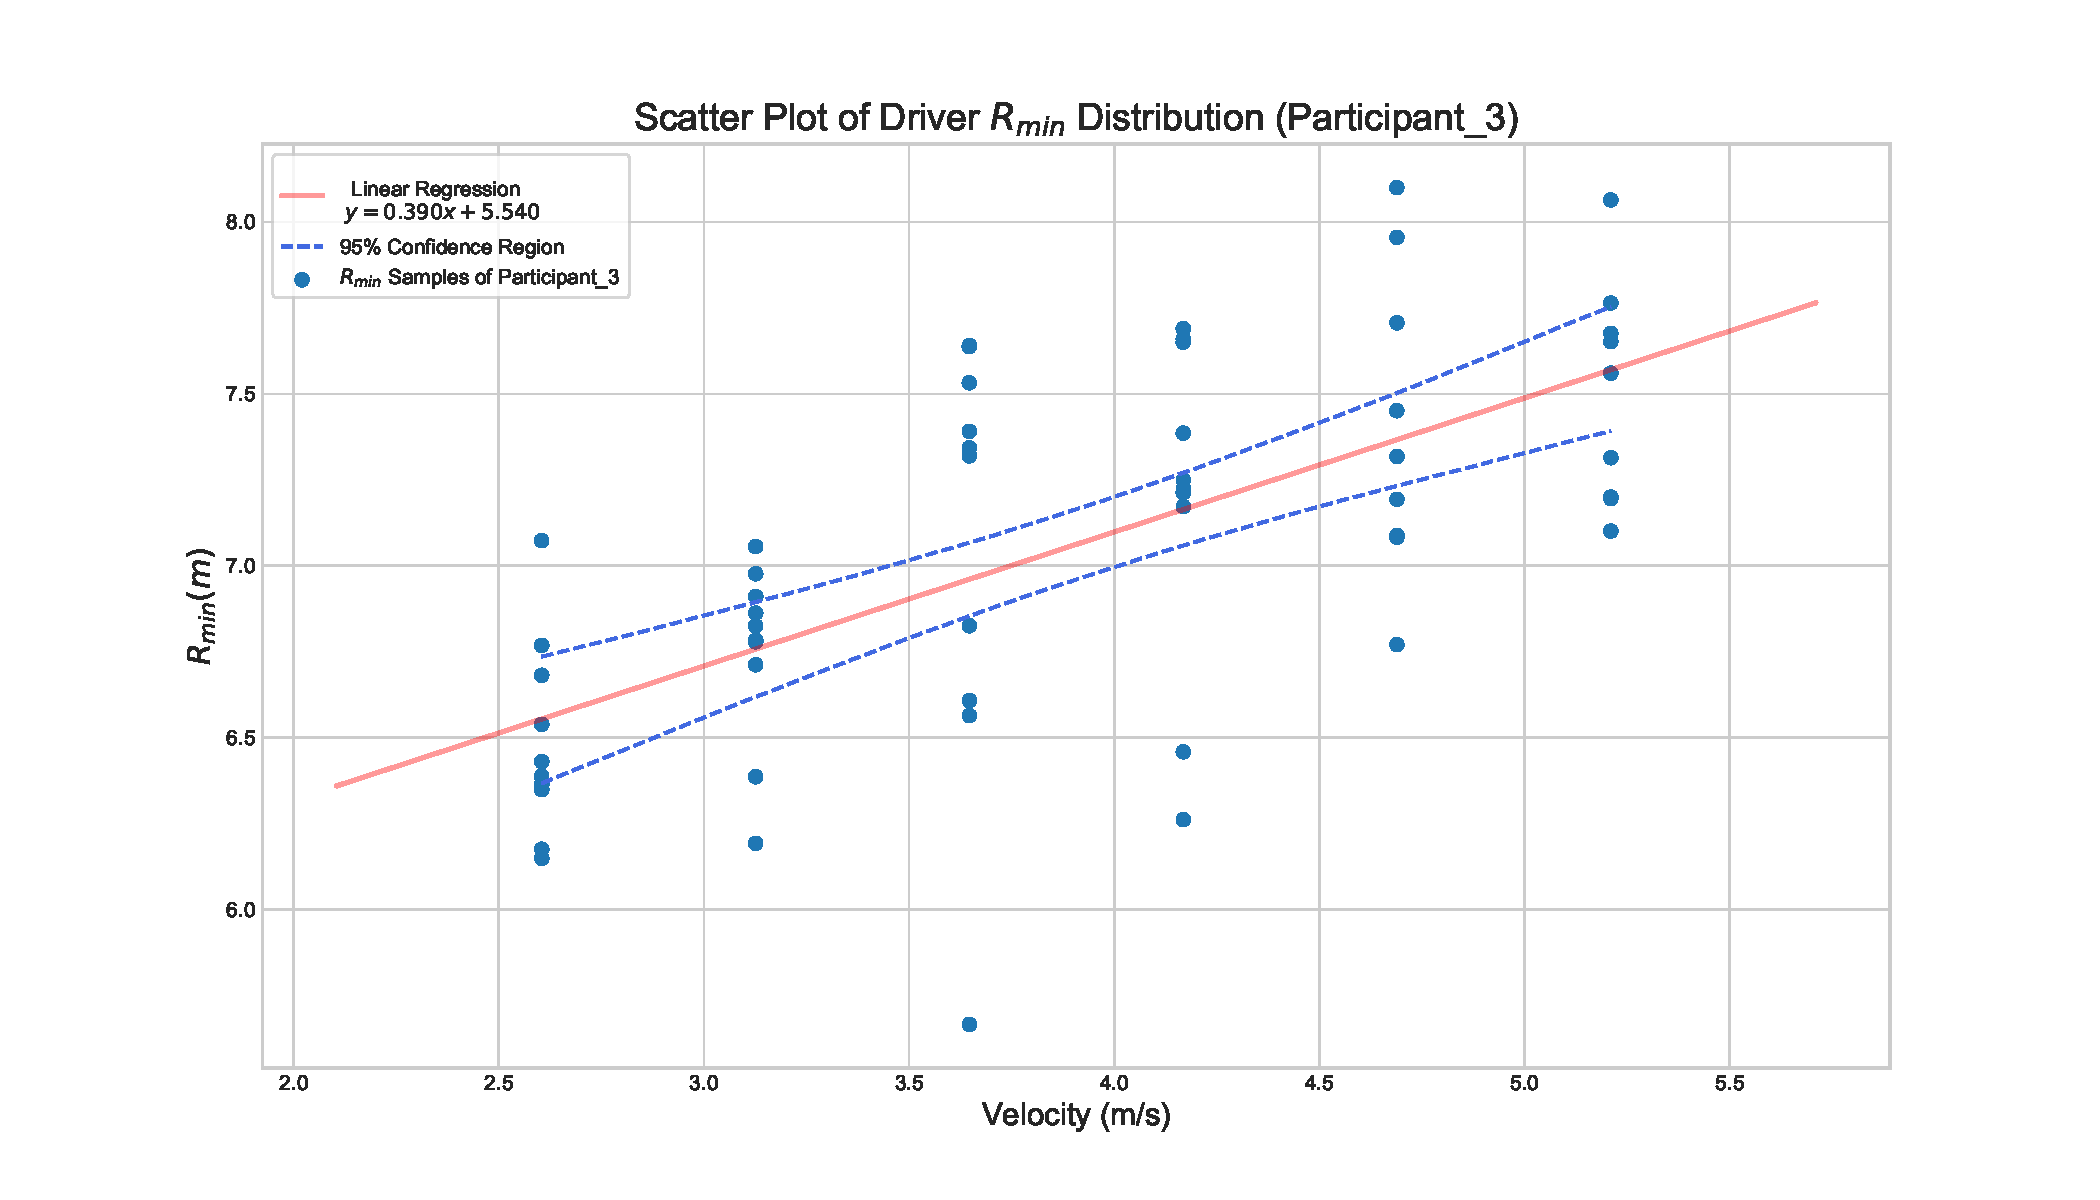
\includegraphics[width=0.7\paperwidth]{/Participant_3_R_MIN_polyfit.pdf}}
\end{center}
\caption{The $R_{min}$ scatter plot of Participant 3 under various velocities.}
\label{fig:Par3RMINDifSpeed} 
\end{figure}

\begin{figure}[htbp!]
\begin{center}
\makebox[0pt]{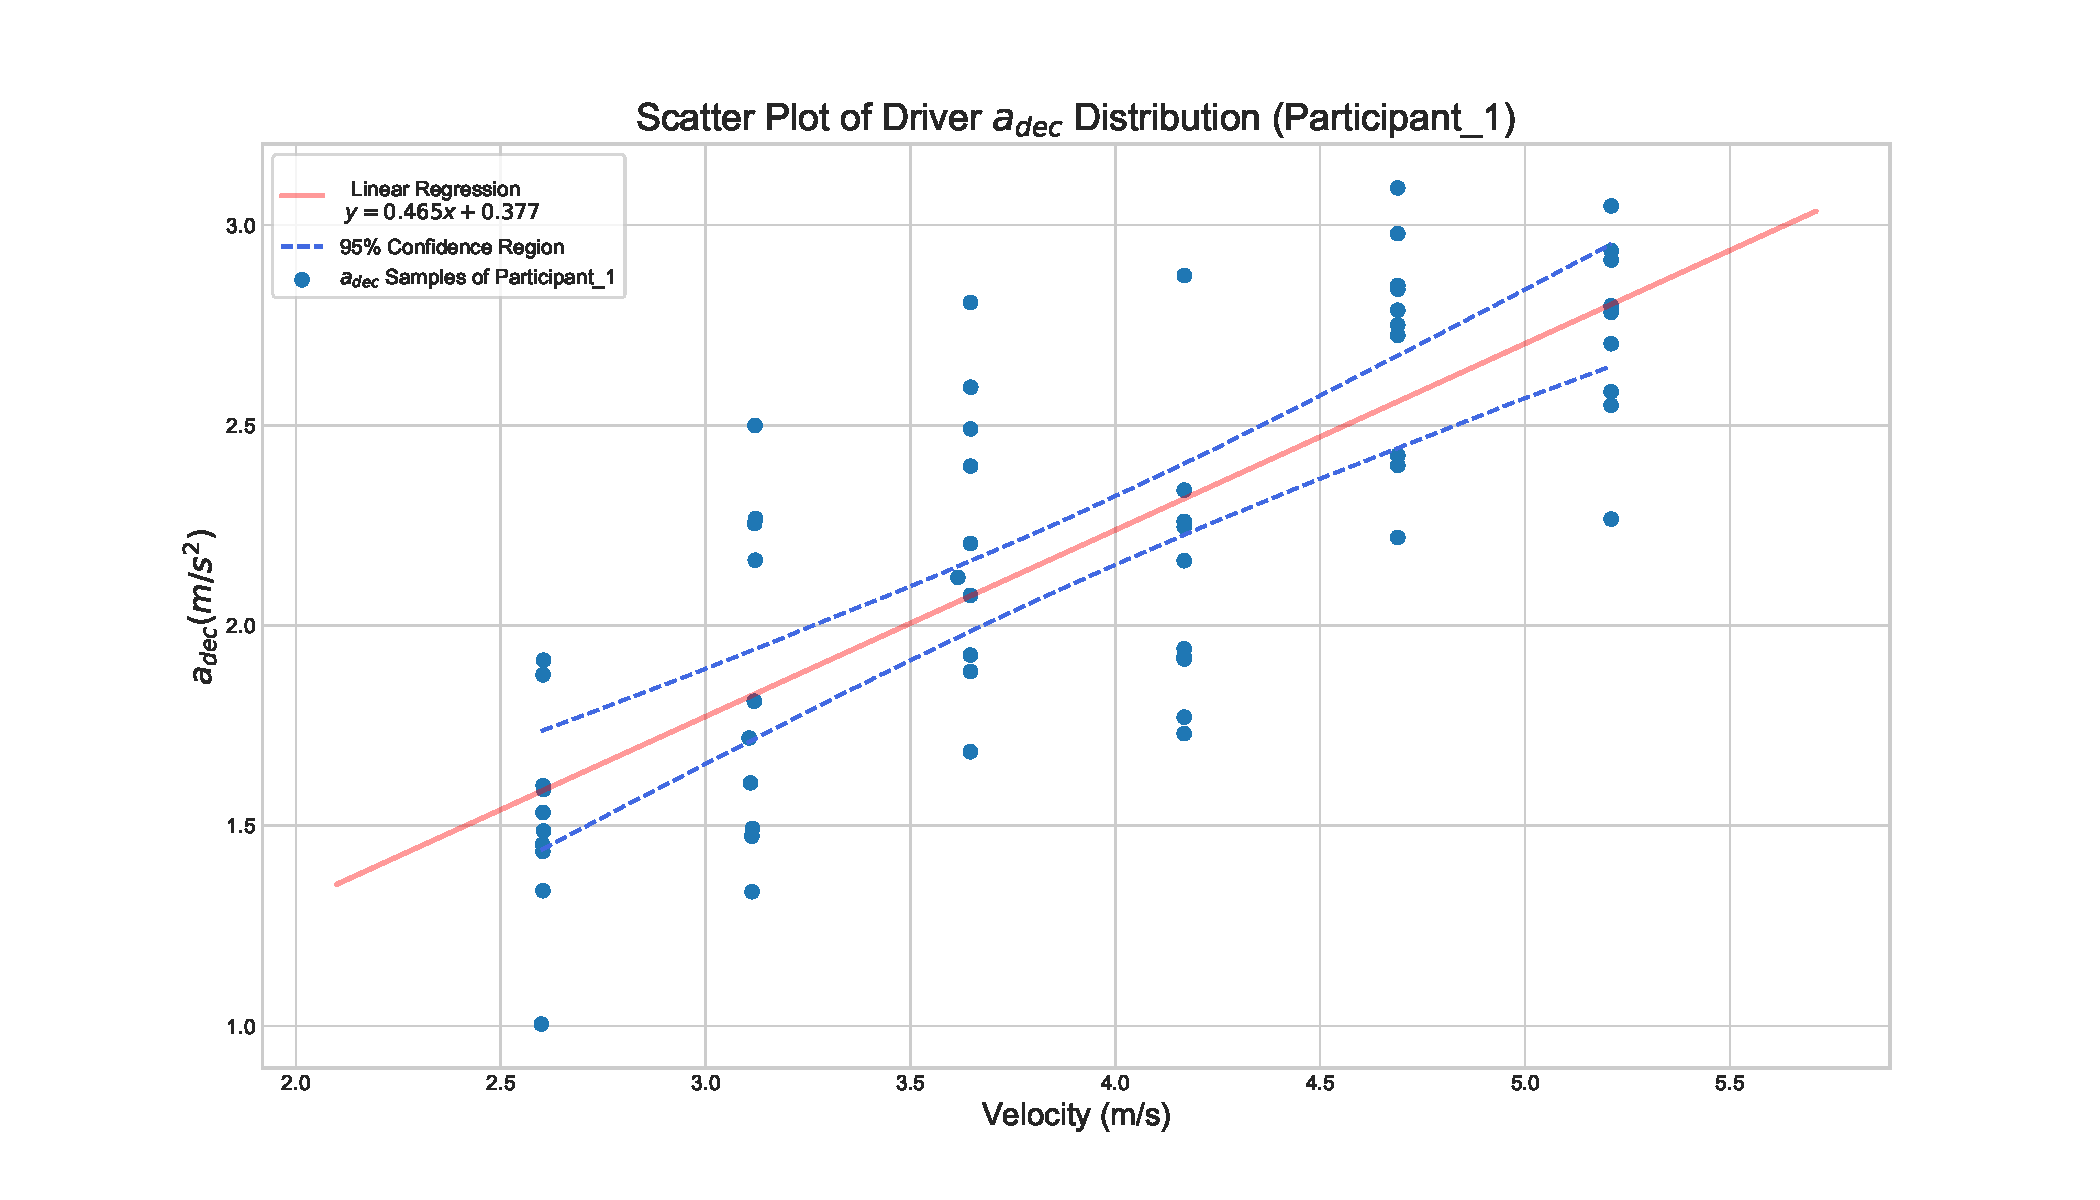
\includegraphics[width=0.7\paperwidth]{/Participant_1_A_DEC_polyfit.pdf}}
\end{center}
\caption{The $a_{dec}$ scatter plot of Participant 1 under various velocities.}
\label{fig:Par1ADECDifSpeed} 
\end{figure}

\begin{figure}[htbp!]
\begin{center}
\makebox[0pt]{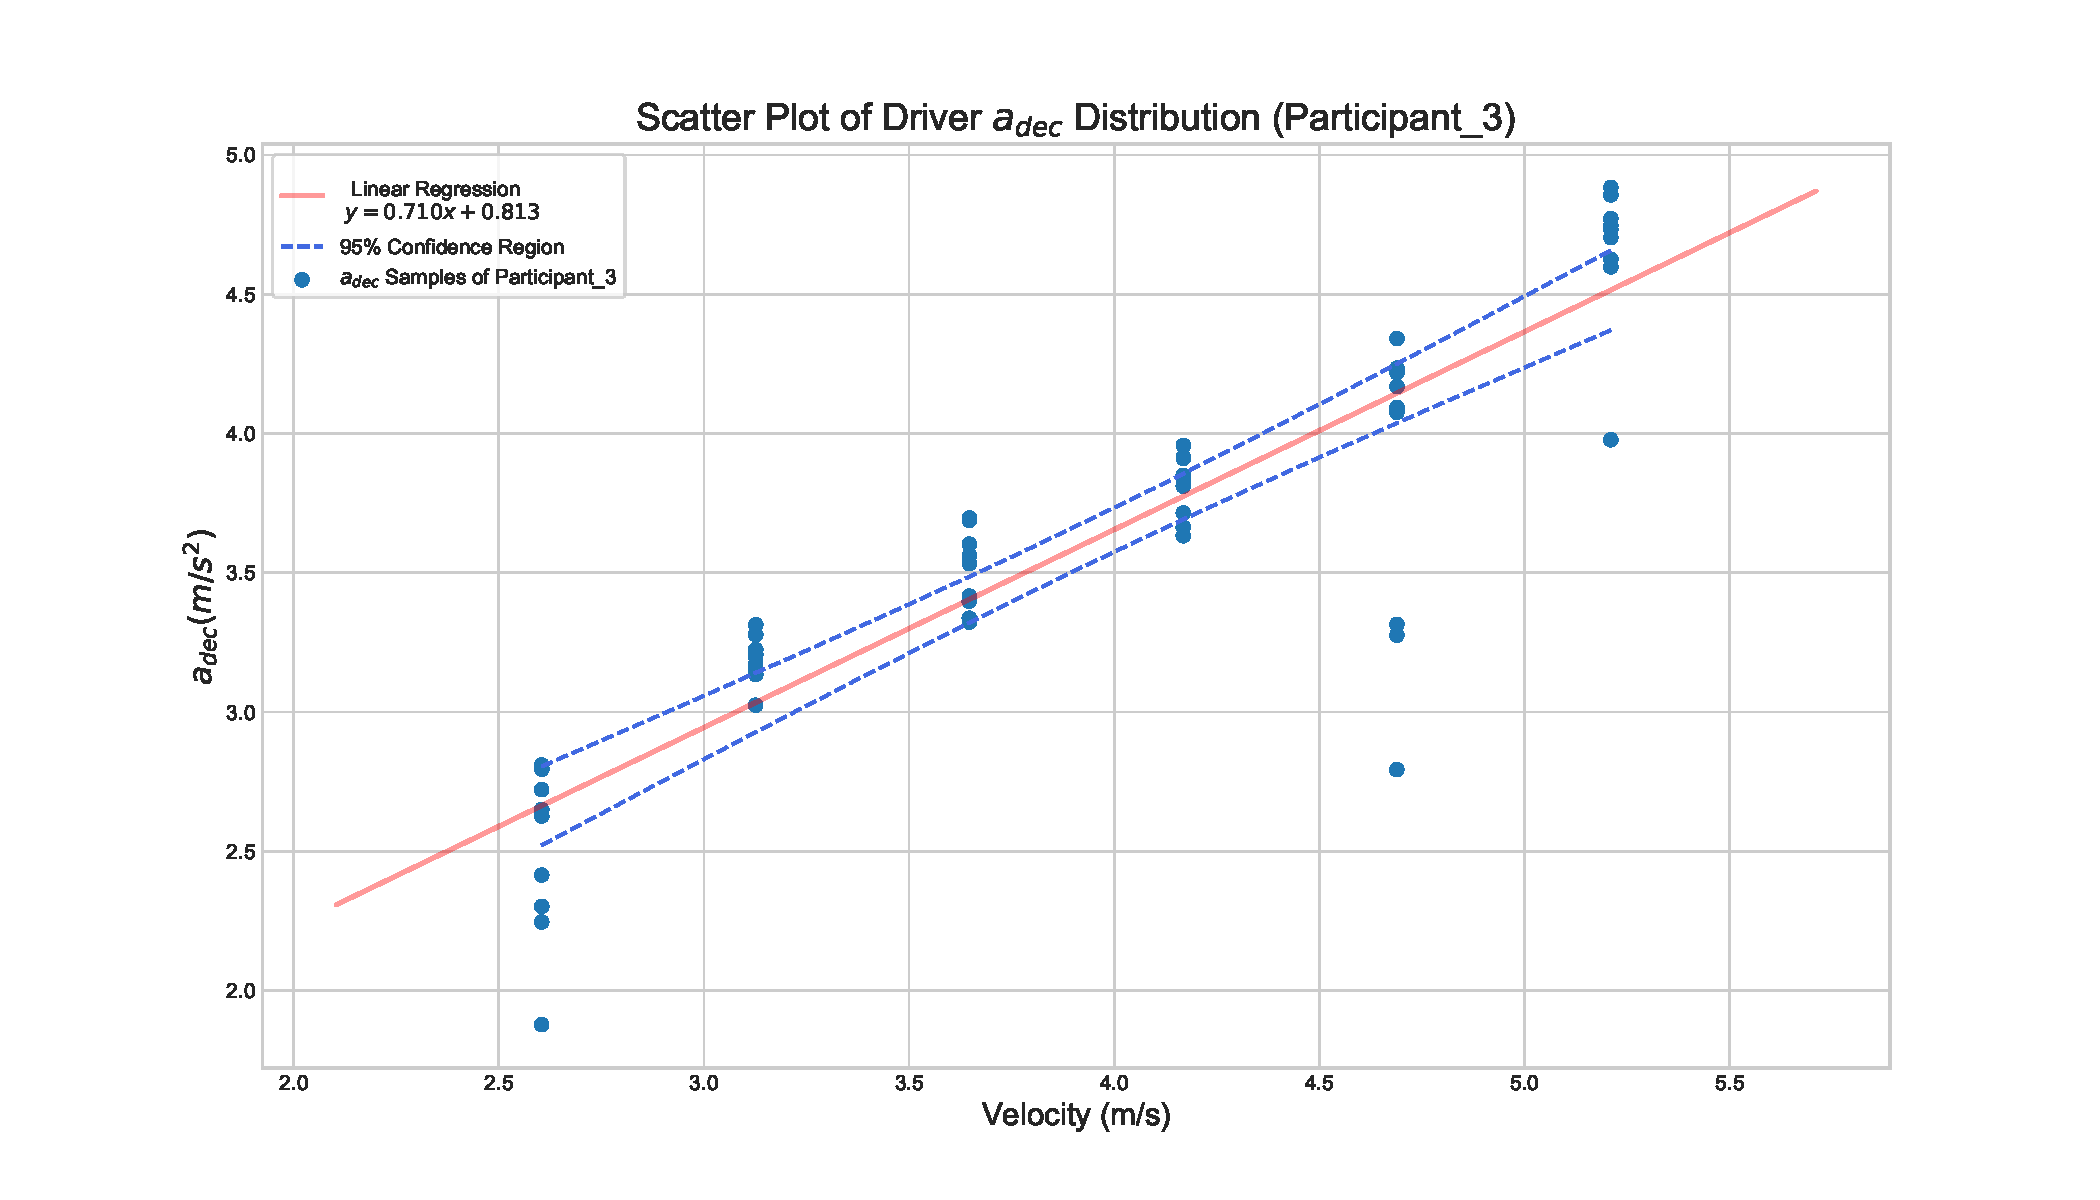
\includegraphics[width=0.7\paperwidth]{/Participant_3_A_DEC_polyfit.pdf}}
\end{center}
\caption{The $a_{dec}$ scatter plot of Participant 3 under various velocities.}
\label{fig:Par3ADECDifSpeed} 
\end{figure}

To identified the corresponding characteristic parameters of participants, experiments same as the one used in Chapter ~\ref{chap:DriverModel} are conducted for each participants. Here, experimental results and characteristic parameters of Participant 1 and 3 are shown in Fig~.\ref{fig:Par1RMINDifSpeed}, Fig~.\ref{fig:Par1ADECDifSpeed}, Fig~.\ref{fig:Par3RMINDifSpeed} and Fig~.\ref{fig:Par1ADECDifSpeed}. 

Similar to the result using combined data of all participants in Chapter ~\ref{chap:DriverModel}, the characteristic parameter of each participant can be approximated linearly and both $R_{min}$ and $a_{dec}$ are positively related to the velocity at the moment. Different values of slopes, as denoted as ${C1}_{Rmin}$ for linear approximated $R_{min}$ or ${C1}_{adec}$ for $a_{dec}$ in Eqn.~\ref{eq:RMIN_Linear} and Eqn.~\ref{eq:ADEC_Linear}, are found on different participants. The values of $R_{min}$, after the intersection at velocity around 3 m/s, those of Participant 3 have higher $R_{min}$ from 3 to 5 m/s. As for $a_{dec}$, the line of Participant 3 is always above that of Participant 1. 

The results can be suggested that Participant 3 is a more cautious driver that Participant 1, since there are larger distances ($R_{min}$ values) left between the vehicle and the obstacle. Combining that with the large $a_{dec}$ values, it is likely that Participant 3 is a new driver (in the simulated traffic environment) since more abrupt brakes are often applied. The characteristic parameters of these two participants are compared with average parameters in Table ~\ref{table:character_average}.

\begin{table}[htbp]
\caption{Table for characteristic and average parameters.}
\begin{center}
\label{table:character_average}
\begin{tabular}{l l c c c}
& & \\ % put some space after the caption
\hline
\textbf{Parameters} &  &\textbf{Average} &\textbf{Participant 1} &\textbf{Participant 3} \\
\hline
Safe Margin Coefficient (${C1}_{Rmin}$)     & & 0.295 & 0.166 & 0.390 \\
Safe Margin Constant (${C2}_{Rmin}$)        & & 5.47 & 6.19 & 5.54  \\
Deceleration Coefficient (${C1}_{adec}$)    & & 0.458 & 0.465 & 0.710 \\
Deceleration Constant (${C2}_{adec}$)       & & 0.877 & 0.377 & 0.813 \\
Standard Diviation Parameter ($\gamma$)     & & 0.148 & 0.115 & 0.102 \\
\hline
\end{tabular}
\end{center}
\end{table}


When the characteristic parameters are identified, it is not only the driving style could be found, the right parameters for the proposed model can also be applied to have a better prediction of the next possible behaviors coming from other traffic participants. In the next section, the CARate curve of average and characteristic parameters will be compared for verification and optimization for the CARate curve will also be employed to identify the matching characteristic parameters. 

%%%%%%%%%%%%%%%%%%%%%%%%%%%%%%%%%%%%%%%%%%%%%%%%%%%%%%%%%%%%%%%%%%%%%%%%
%%%%%%%%%%               SECTION SECTION SECTION               %%%%%%%%%
%%%%%%%%%%%%%%%%%%%%%%%%%%%%%%%%%%%%%%%%%%%%%%%%%%%%%%%%%%%%%%%%%%%%%%%%
\section{Objective Function and Constraints for Optimization}
\label{sec:optim_obj_con}

In Section ~\ref{sec:characterParam}, the POY curves of the same trial using different variables sets are found to be different, because a more accurate approximation to the TFA distribution is generated using the characteristic parameters of the driver. To compare the characteristic parameters of a particular driver to average parameters, the trials involving that driver are specified and used as the database for the CARate curves using two sets of parameters. Results are plotted in Fig.~\ref{fig:CAR_comparison}.


\begin{figure}[htbp!]
\begin{center}
\makebox[0pt]{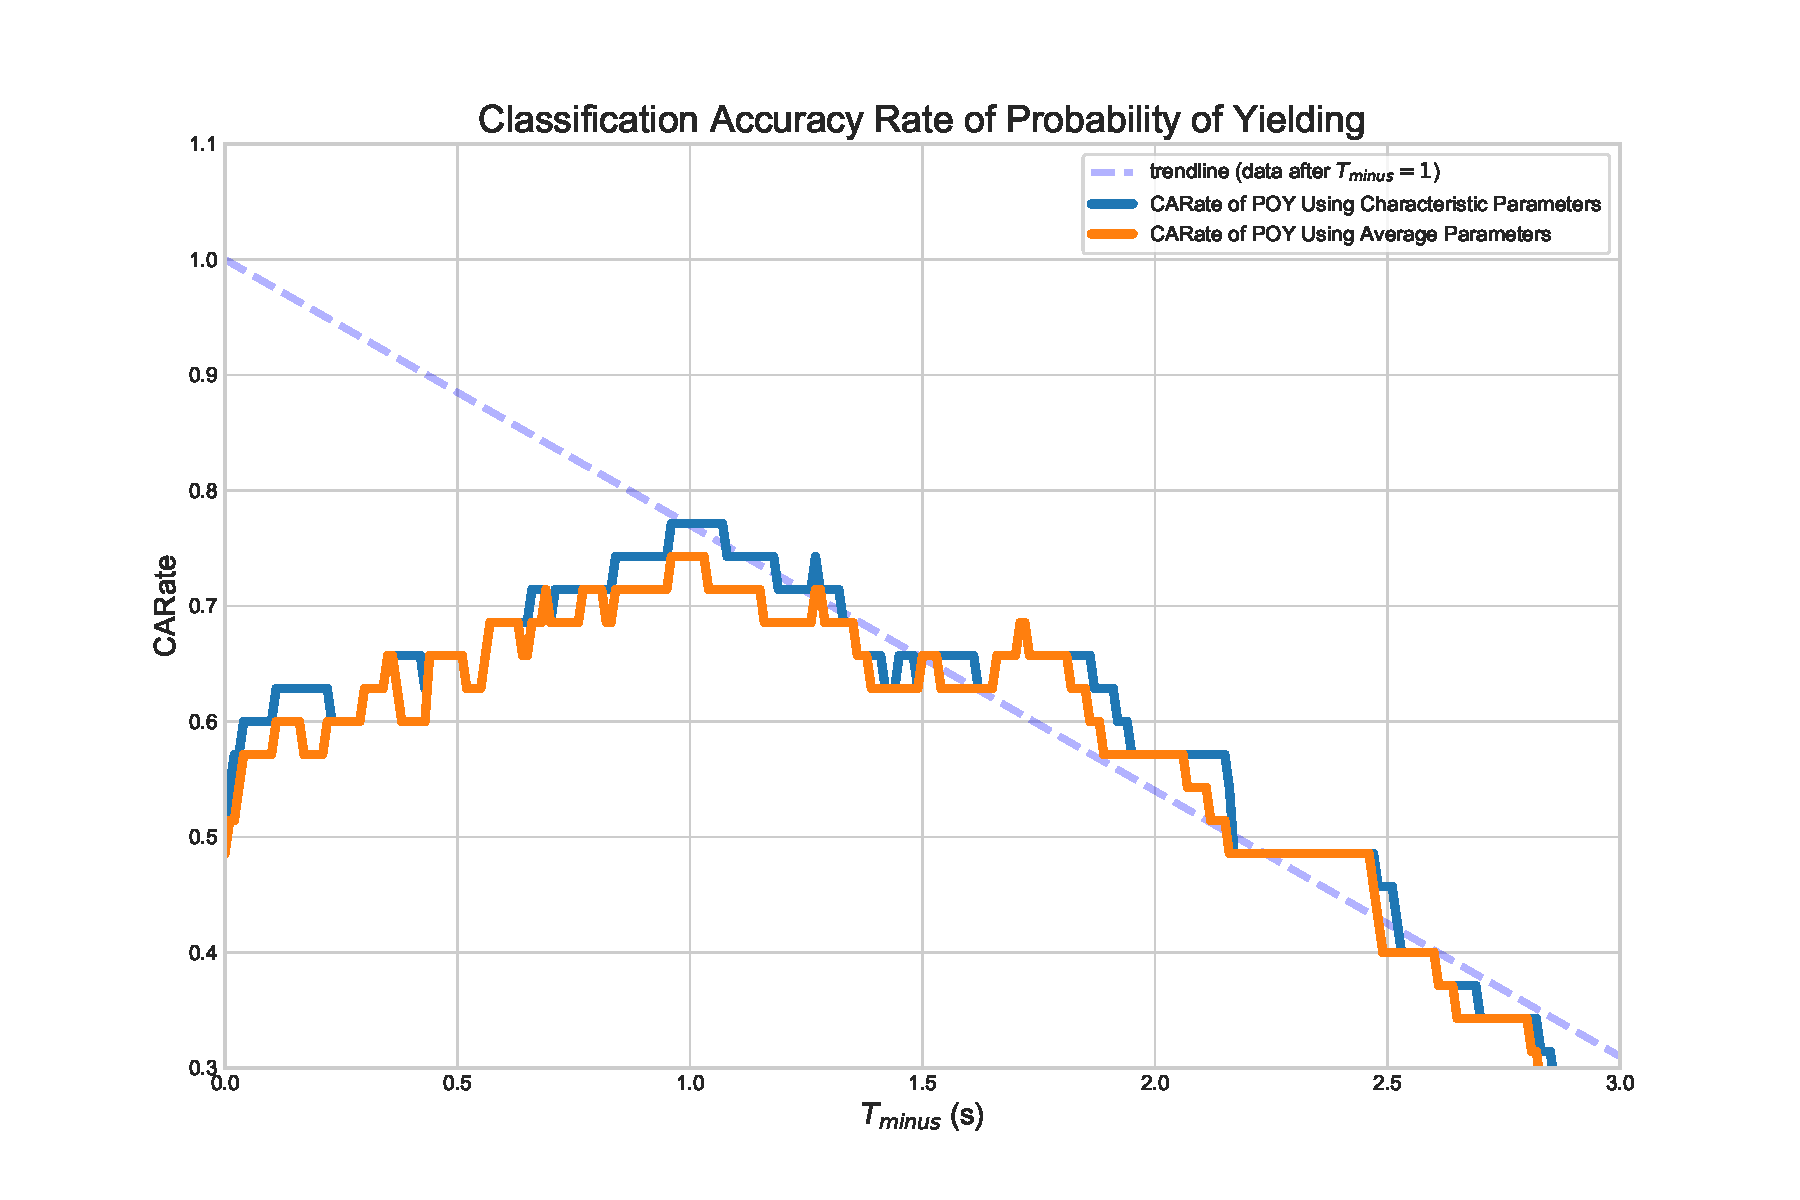
\includegraphics[width=0.7\paperwidth]{CARPOY_character_average.pdf}}
\end{center}
\caption{CARate curve of POY using average parameters and characteristic parameters are compared.}
\label{fig:CAR_comparison} 
\end{figure}


In the figure, the solid blue line indicates the CARate curve of POY using characteristic parameters (blue line for short ) while the orange line represents the CARate curve of POY using average parameters (orange line for short). The highest CARate of the blue line is around 0.78, which is higher than that of the orange line around 0.74. Despite the non-significant difference between two highest points, it is noticable that blue line is above the orange line throughout the whole $T_{minus}$ span, which gives the evidence to the supposition that the closer parameters set can give rise to larger area under the resulting CARate curve. If a more far off set of parameters are applied, e.g. the parameters set of another participant, the gaps between the resulting CARate cure of POY should be larger, owing to the more imprecise estimation for the TFA distribution. The comparison between the characteristic parameters and the parameters set of another participants are made in Fig.~\ref{fig:CAR_twoParticipants}.


\begin{figure}[htbp!]
\begin{center}
\makebox[0pt]{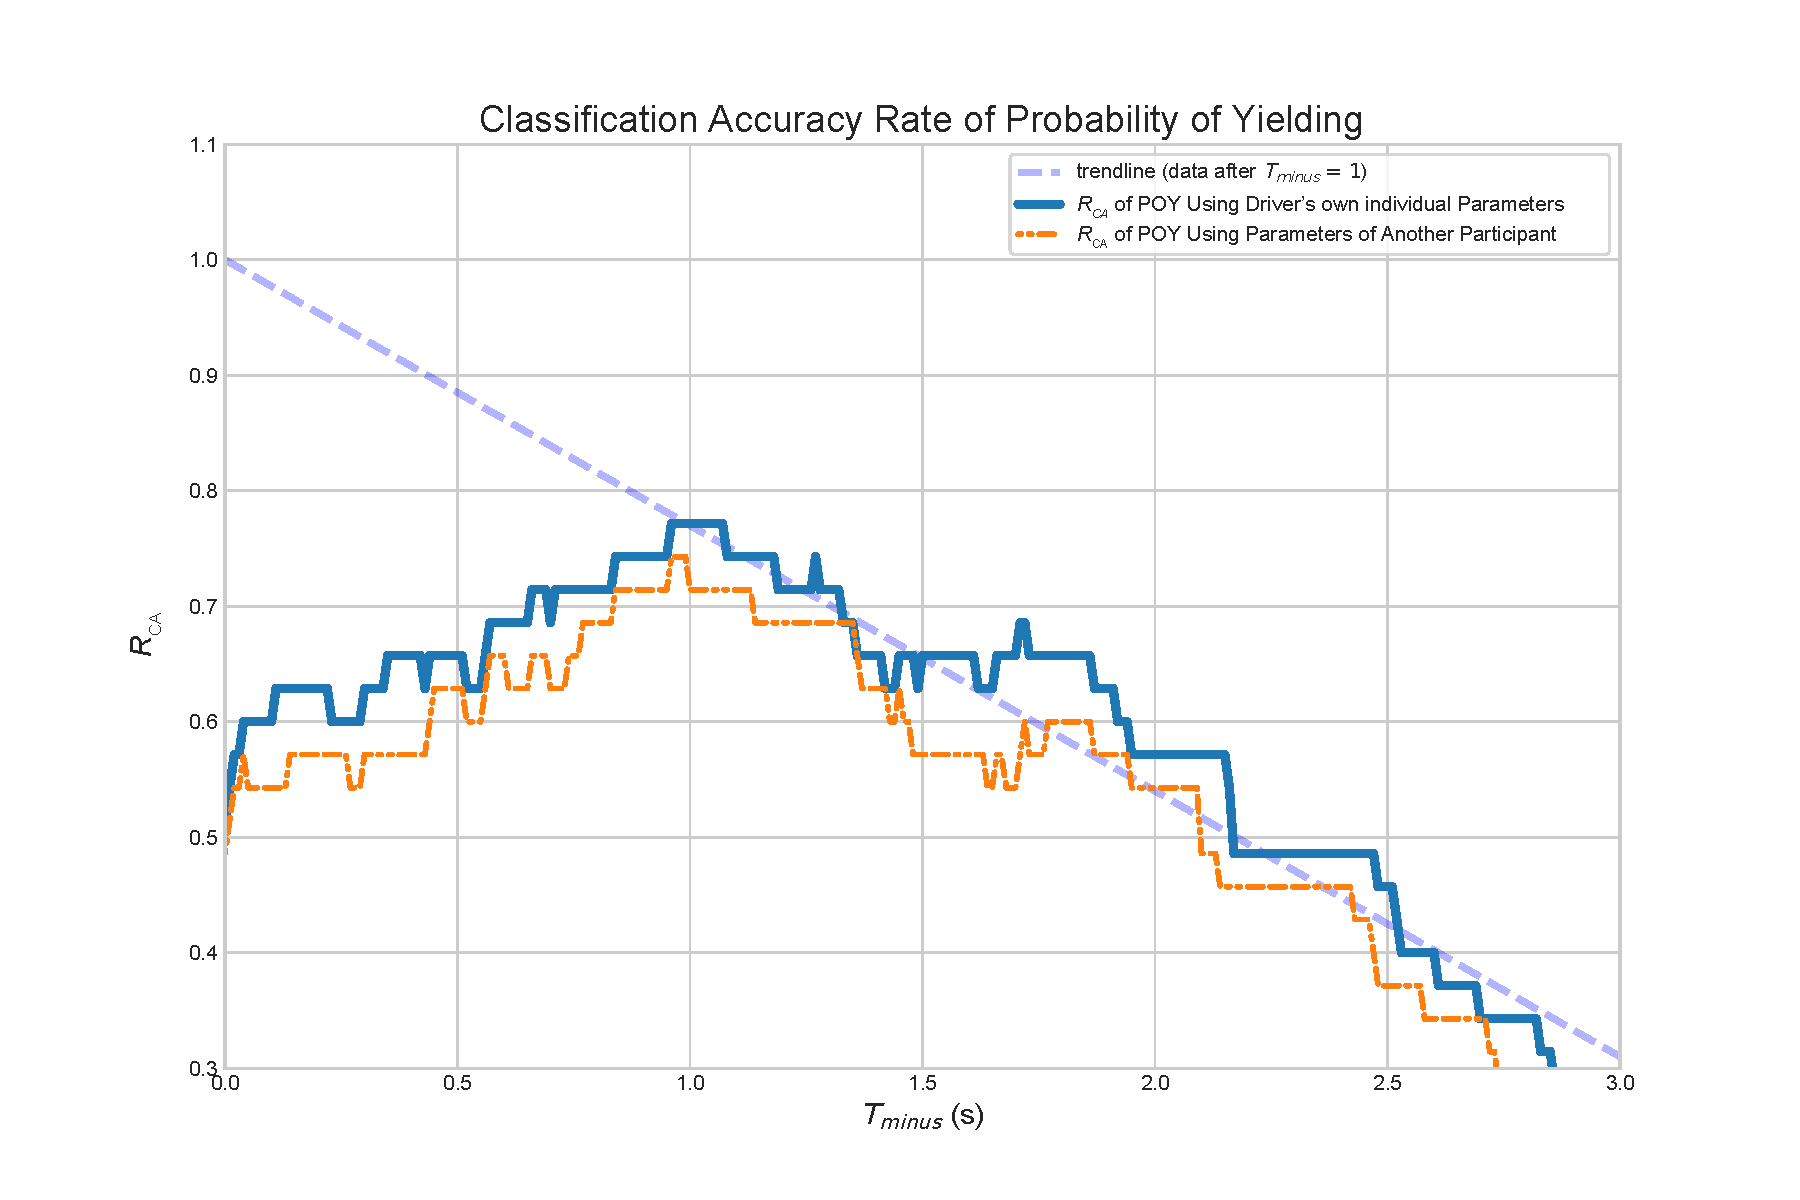
\includegraphics[width=0.7\paperwidth]{CARPOY_twoParticipants.pdf}}
\end{center}
\caption{CARate curve of POY using characteristic parameters and the parameters set of another participant are plotted.}
\label{fig:CAR_twoParticipants} 
\end{figure}

It is not hard to observe that the differences between two CARate curves are more distinct than that in Fig.~\ref{fig:CAR_comparison}, for that the values of average parameters set is closer to characteristic parameters than that of another participant.

Up to the present, the differences between the resulting CARate curves using different sets of parameter are identified. Based on this idea, creating a procedure using collected traffic data at crossroad to identify the characteristic parameters representing the driving behaviors of that area is possible. So the problem now would be, how to optimize the CARate curve so as to find the most possible parameters set representing the driver.

To solve the problem using optimization, the objective function and constraints are defined as 


    \begin{mini}|l|
	  {w}{\frac{1}{M}~\sum_{j=1}^{M}\sum_{i=1}^{N_j}{- f( { POY}_{j}(t_i, w))}}{}{}
	  \addConstraint{~2.0 \cdot {C1}_{Rmin}+{C2}_{Rmin}~}{\geq ~ 4.48}{}
	  \addConstraint{~5.2 \cdot {C1}_{Rmin}+{C2}_{Rmin}~}{\leq ~ 12.0 }{}
	  \addConstraint{~2.0 \cdot {C1}_{adec}+{C2}_{adec}~}{\geq ~ 0.01}{}
	  \addConstraint{~5.2 \cdot {C1}_{adec}+{C2}_{adec}~}{\leq ~ 3.5 }{}
	  \addConstraint{0.01~ \leq~ \gamma ~\leq ~ 0.5}{ }{}
     \label{eq:optimize_POY}
     \end{mini}

\noindent where the function ${POY}_{j}$ in the optimization problem is

\begin{equation}
    f({POY}_{j}) = 
    \begin{cases} 
      1 &~~\text{if}~~ {POY}_{j}(t, w)~\geq~0.8~\text{and yielded}~ \\
      1 &~~\text{if}~~ {POY}_{j}(t, w)~\leq~0.2~\text{and passed}~ \\
      0 &~~\text{otherwise}
    \end{cases}
\label{eq:POY_j_condition}
\end{equation}

The objective function in Eqn.~\ref{eq:optimize_POY} indicating the total area underneath the CARate curve, where the $w$ is the parameters set ($R_{min}, a_{dec}, \gamma $) maximizing the area (minimizing the negative area), i.e., bringing the parameters set into the proposed POY model could have the highest accuracy on predicting the behaviors of the driver from the experimental data. The constants $M$ and $N_j$ stand for the number of the trials in the collected data and the number of time steps in each trial with the resolution of 0.01 sec.

Due to the linearity of $R_{min}$ and $a_{dec}$, the maximum and minimum value of both parameters should occur at the maximum and minimum velocity right before braking which are 5.2 and 2.0 m/s respectively. While the definition of the $R_{min}$ is calculated from the center of one vehicle to another, the minimum distance under 2.0 m/s is also bounded by the physical model built in the simulated world, which is 4.48 meters. The maximum is then bounded by the longest between vehicles one could possibly have, which is 12 meters, the maximum distance they can see each other. As for the minimum and maximum in the constraint of $a_{dec}$, they are also restraint within the boundary set for the commend velocity sent from the joystick, which are 0.01 and 3.5 respectively.

%%%%%%%%%%%%%%%%%%%%%%%%%%%%%%%%%%%%%%%%%%%%%%%%%%%%%%%%%%%%%%%%%%%%%%%%
%%%%%%%%%%               SECTION SECTION SECTION               %%%%%%%%%
%%%%%%%%%%%%%%%%%%%%%%%%%%%%%%%%%%%%%%%%%%%%%%%%%%%%%%%%%%%%%%%%%%%%%%%%
\section{Optimization Using Simulated Annealing}
\label{sec:simAnneal}


In this research, the \ac{SA} is chosen for this optimization problem due to the non-smooth and time-consuming properties of the objective function. First published by Kirkpatrick et al. \cite{Kirkpatrick1983}, \ac{SA} is an efficient method to approximate the global optimization without using the derivative information. Despite being a global optimizer, it is not guaranteed that the solution found is an global optimum, however, the close enough variables set within limited time could be discovered.

The process of \ac{SA} is an inspiration from the annealing process in material science, where the ductility is increased during the cooling process. The key idea applied to the optimization problems is the process of the temperature dropping, which is redefined as the lowering probability of accepting a worse variables set as the solution in the optimization problem. Four essential elements in the \ac{SA} optimization problem are listed below :

\begin{itemize}

    \item \textbf{Energy function} : \\
        Usually denoted as $E_i$, representing the value of objective function using the best solution (set of variables) at the moment. In this situation, the sign of $\Delta E$ is then defining the current $move()$ to be an uphill or a downhill move.
        
    \item \textbf{Random number generator} :\\
        The function $move()$ update the solution for the optimization problem. Despite the Monte Carlo method is applied, a well defined update procedure can solve the optimization problem with efficiency.
        
    \item \textbf{Worse case accepting probability} :\\ 
        Defining the probability $P_i$ that whether to accept a worse solution is the essential element for the \ac{SA} to jump out of the local minimum. It is usually in the form of
        
        \begin{equation}
             P_i = \exp{\frac{- \Delta E}{T_i}}
        \label{eq:SA_tempDrop}
        \end{equation}
    
        where the $\Delta E$ represents the difference between the objective function value generated by the new solution and the best one so far. When a worse solution is generated, the value $P_i$ is compared to a random number, and the worse solution is accepted if $P_i$ is greater than the random number. Hence, larger the $\Delta E$ values will reduce the chance a worse solution being accepted. On the contrary, higher the current temperature indicating a higher chance of adopting the worse solution.
    
    \item \textbf{Annealing ( cooling ) schedule} : \\
        Within the \ac{SA}, the temperature drop is governed by equation

        \begin{equation}
             T_{i+1} = T_{i} \cdot \exp{\frac{T_{factor, i} \cdot i}{N}}
        \label{eq:SA_tempDrop}
        \end{equation}

        where the $T_{factor}$ is defined as

        \begin{equation}
            T_{factor, i} = - \ln{\frac{T_{i}}{T_{min}}}
        \label{eq:SA_tFactor}
        \end{equation}

        The temperature decay is based on the Newton's law of cooling with little modification to end the optimization process within designated number of steps $N$. In the equation, the $T_i$ is the current temperature and $T_min$ is the target temperature of cooling ( i.e. the environment temperature in the annealing process ). 
\end{itemize}

In our case, the energy function $E_i$ is defined by the objective function in Eqn.~\ref{eq:optimize_POY}, where the $\Delta E$ is found in every iteration by calculating $(E_{i+1} - E_i)$ after the new set of variables are generated by function $move()$ and examined to satisfy the constraints. If a better solution is found ( meaning that $\Delta E < 0$ ), the best solution is replaced with the new one. Otherwise, the probability $P_i$ is then compared to a random number to decide whether to accept the worse solution. The process then iterate $N$ times (until the temperature drops to the environment temperature), or one of the termination conditions is reached. 

The results of the optimization are shown in Table ~\ref{table:SAresults}, and the parameters used for the \ac{SA} in the optimization problem are listed in Table ~\ref{table:SAparams}.


\begin{table}[htbp]
\caption{Table for results of the proposed optimization problem.}
\begin{center}
\label{table:SAresults}
\begin{tabular}{l l c c c c c c}
& & \\ % put some space after the caption
\hline
\textbf{Optimization Number} &  &\textbf{${C1}_{Rmin}$} &\textbf{${C2}_{Rmin}$} &\textbf{${C1}_{adec}$} &\textbf{${C2}_{adec}$} & \textbf{$\gamma$} & \textbf{Area}\\
\hline
1st Optimization  &  & 0.362 & 7.91 & 0.0460 & 0.954 & 0.460 & -205.40 \\
2nd Optimization  &  & 0.401 & 7.86 & 0.224 & 0.563 & 0.443 & -205.37 \\
3rd Optimization  &  & 0.322 & 7.91 & 0.106 & 0.941 & 0.434 & -205.23 \\
4th Optimization  &  & 0.456 & 7.49 & 0.102 & 0.824 & 0.444 & -205.37 \\
5th Optimization  &  & 0.346 & 7.95 & 0.145 & 0.812 & 0.448 & -205.37 \\
\textbf{Characteristic}  &  & \textbf{0.166} & \textbf{6.19} & \textbf{0.465} & \textbf{0.377} & \textbf{0.114} & \textbf{-183.89} \\
\hline
\end{tabular}
\end{center}
\end{table}

\begin{table}[htbp]
\caption{Table for parameters used in the Simulated Annealing.}
\begin{center}
\label{table:SAparams}
\begin{tabular}{l l c c c}
& & \\ % put some space after the caption
\hline
\textbf{Parameters} &   & Values \\
\hline
Start Temperature    &  120  \\
End Temperature      &  0.02 \\
Steps                & 100000 \\

\hline
\end{tabular}
\end{center}
\end{table}

\begin{figure}[htbp!]
\begin{center}
\makebox[0pt]{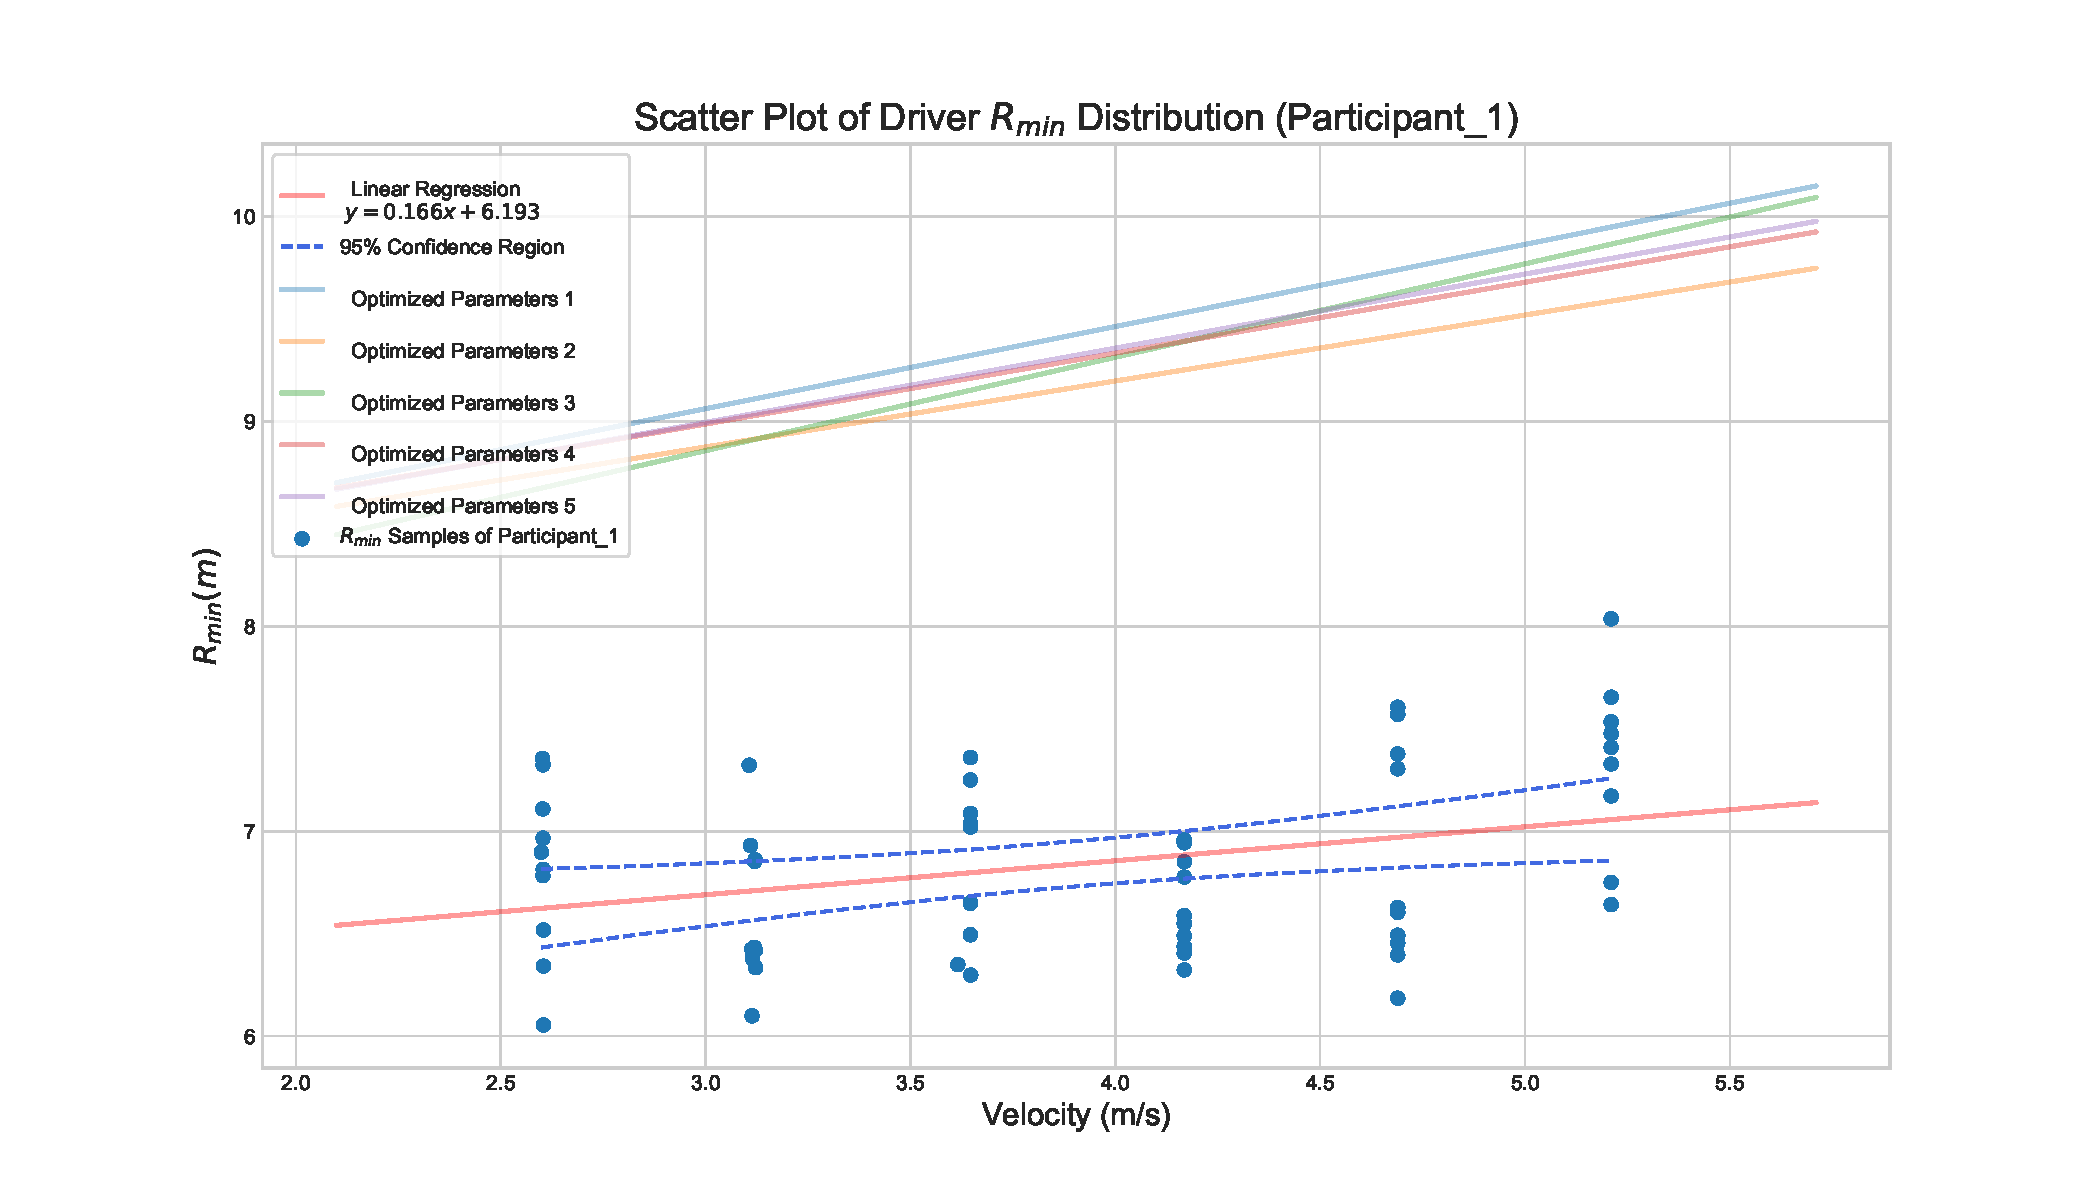
\includegraphics[width=0.7\paperwidth]{Participant_1_R_MIN_optimized.pdf}}
\end{center}
\caption{Optimized parameters of $R_{min}$ are compared with characteristic parameters.}
\label{fig:RMINParamOptimChara} 
\end{figure}

\begin{figure}[htbp!]
\begin{center}
\makebox[0pt]{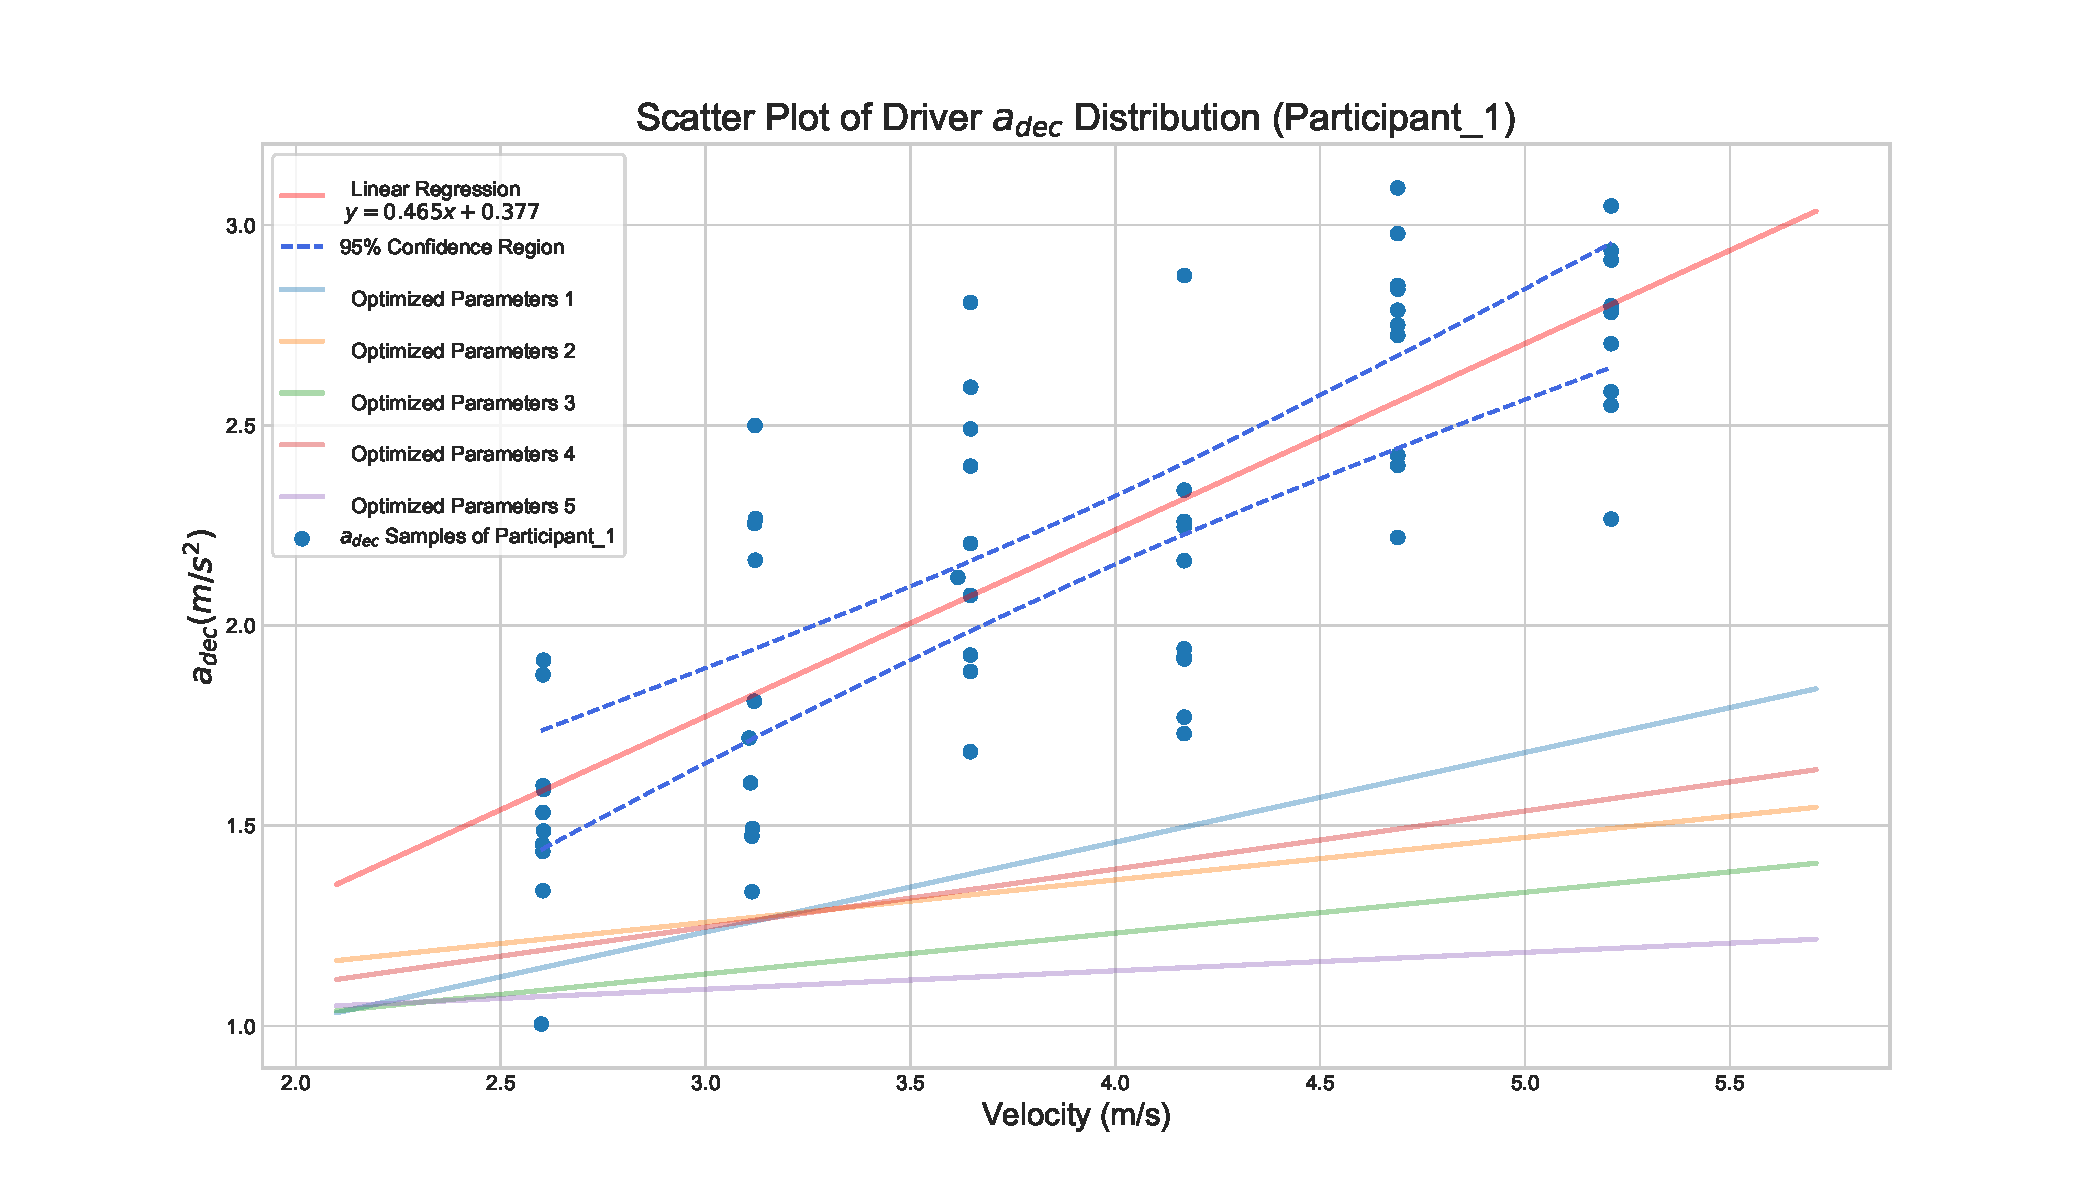
\includegraphics[width=0.7\paperwidth]{Participant_1_A_DEC_optimized.pdf}}
\end{center}
\caption{Optimized parameters of $a_{dec}$ are compared with characteristic parameters.}
\label{fig:ADECParamOptimChara} 
\end{figure}

The optimized parameters for $R_{min}$ and $a_{dec}$ are shown in Fig.~\ref{fig:RMINParamOptimChara} and Fig.~\ref{fig:ADECParamOptimChara}.While in Fig.~\ref{fig:CAR_optimParam}, the CARate curves using optimized parameters listed in Table ~\ref{table:SAresults} are plotted together with the CARate curves using characteristic parameters. In Fig.~\ref{fig:RMINParamOptimChara} and Fig.~\ref{fig:ADECParamOptimChara}, the corresponding lines representing the linear equation using ${C1}$ and $C2$ as the coefficient and constant are forming a cluster in plots of $R_{min}$. While in $a_{dec}$, the lines are not as ordered at higher velocities. 


However, when looking into Fig.~\ref{fig:CAR_optimParam}, all of the optimized CARate curves are overlapped and the area under the curves are larger than the characteristic parameters. Some might wonder, does this implied that the optimized parameters are a better set of parameters that can explain the behavior of the driver? To answer this question, first, the POY curves using the optimized parameters should be examined.

\begin{figure}[htbp!]
\begin{center}
\makebox[0pt]{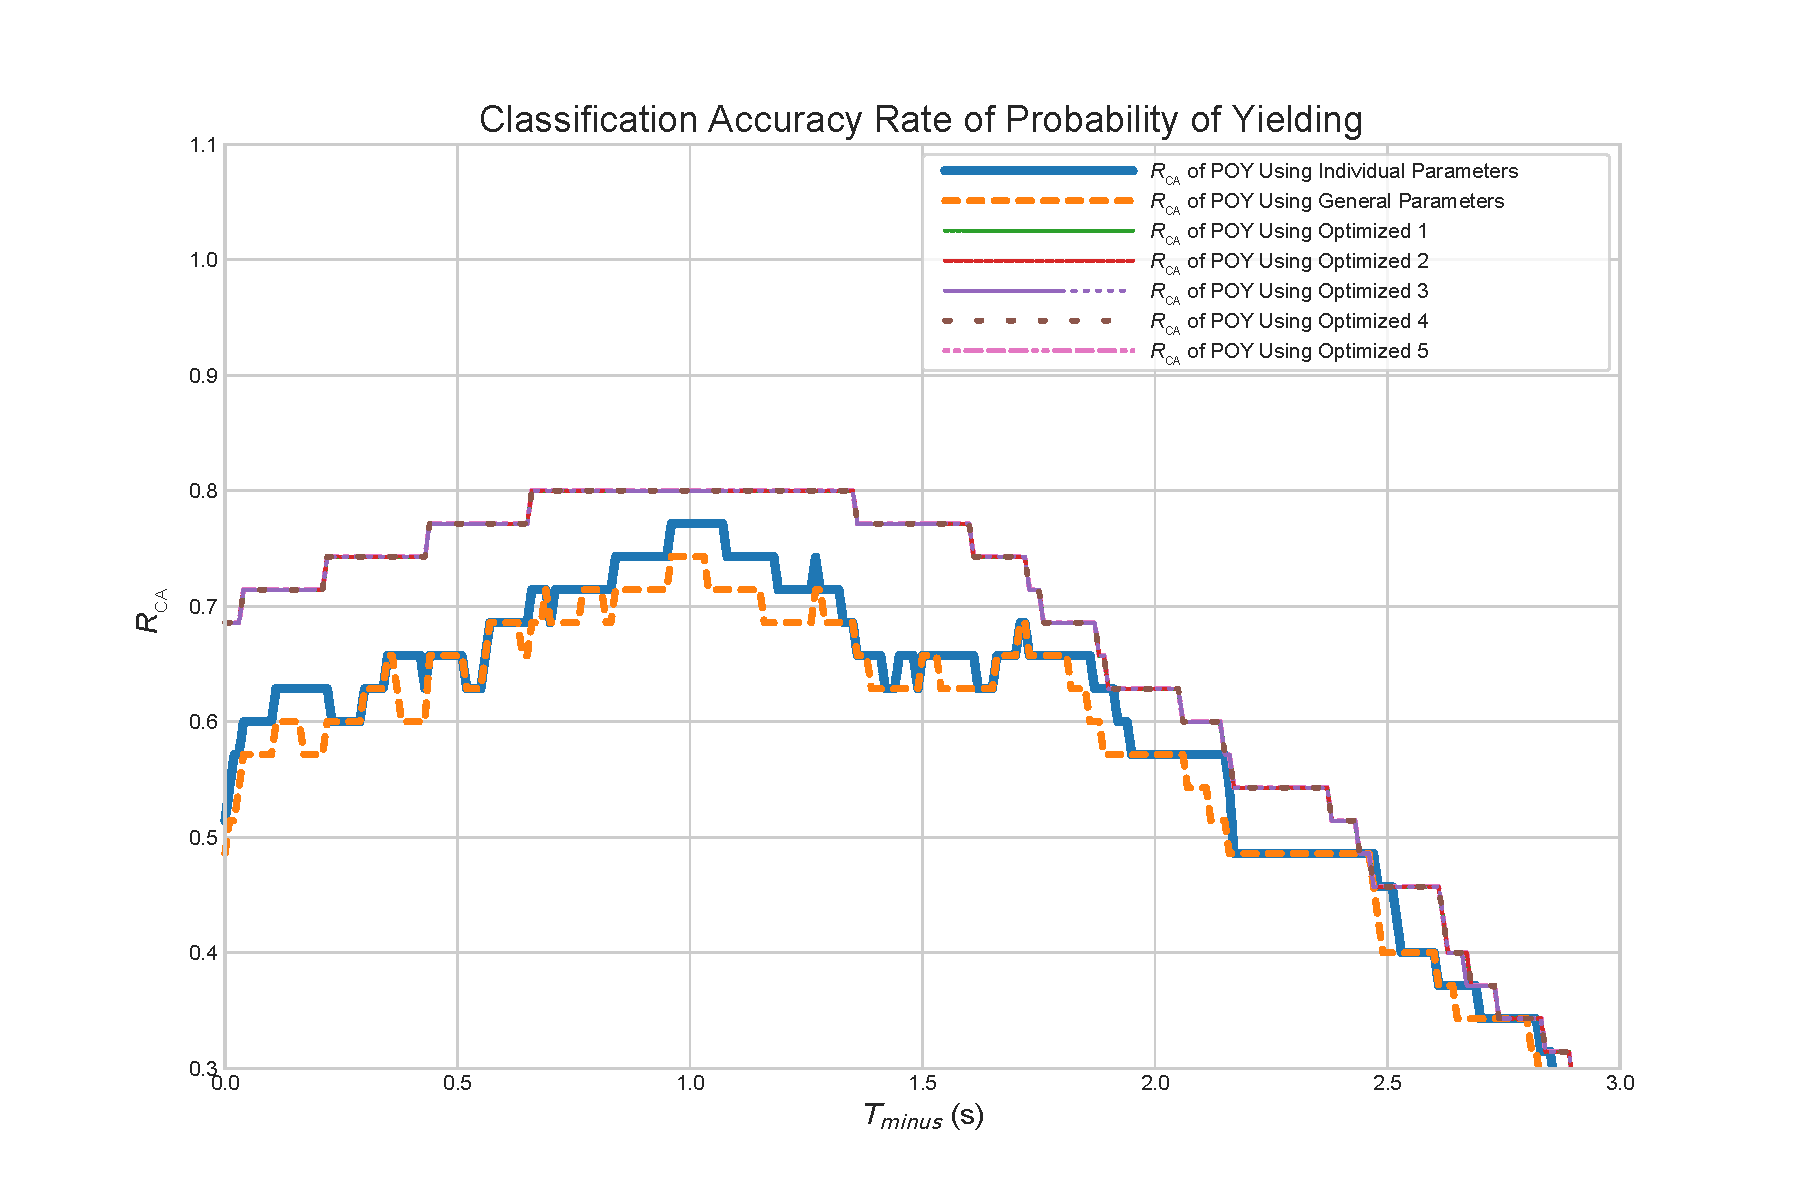
\includegraphics[width=0.7\paperwidth]{CARPOY_optimizedParam.pdf}}
\end{center}
\caption{CARate curve of POY using characteristic parameters and optimized parameters are plotted.}
\label{fig:CAR_optimParam} 
\end{figure}

As shown in Fig.~\ref{fig:trial003OptimChara} and Fig.~\ref{fig:trial077OptimChara}, the POY curves of the optimized parameter (here the parameters set Optimized 1 is chosen ) rose way earlier than using the characteristic parameters. This implies that the the POY with optimized parameters is very sensitive to all the accelerations, so at the instance the vehicle begins to decelerate, the action is considered as having the intention to yield. Yet, being too sensitive to accelerations will result in the bumpy curves, making the meaning of POY curves not understandable, and will sometimes generate false results. For example, the rises of POY curves using optimized curves in both figures are way early than the interactions begin, which happen around the distance to the node is about 15 meters. The optimized parameters do have a better CARate curve, but this does not suggest a more accurate prediction. Some modifications for the objective function are required, so the characteristic parameters could be identified more accurately.


\begin{figure}[htbp!]
\begin{center}
\makebox[0pt]{\includegraphics[width=0.7\paperwidth]{optimized_trial_003.pdf}}
\end{center}
\caption{Trial \#003 using the optimized parameters and the characteristic parameters.}
\label{fig:trial003OptimChara} 
\end{figure}

\begin{figure}[htbp!]
\begin{center}
\makebox[0pt]{\includegraphics[width=0.7\paperwidth]{optimized_trial_077.pdf}}
\end{center}
\caption{Trial \#077 using the optimized parameters and the characteristic parameters.}
\label{fig:trial077OptimChara} 
\end{figure}


In this chapter, a characteristic parameters identification procedure was developed. From the examinations of the POY curves using the characteristic parameters of the driver and the average parameters, the idea of using the results of POY curves and CARate curves to identify the characteristic parameters was generated. After proving it using the CARate curve, an optimization problem was constructed with the area under the CARate curve as the objective function. Despite some improvements are needed to have a more precisely parameters identification, this procedure provides a preliminary method for characteristic parameters recognition.

\chapter{Applications}
\label{chap:App}
\resetfigpath{Chap5}

%%%{INTRODUCTION to this CHAPTER}%%%
In this chapter, the applications of the proposed driver behavior model are presented. In the first application, the relationship between certain driver behaviors and crashing cases are identified. Then, the proposed model is applied to predict the behaviors of drivers at an urban crossroad in real world where the performance is also evaluated. For the second application, considering that in the near future, it will be urgent for autonomous vehicles to handle the stnad-off situation where both participants are having the intention to yield (or to pass). To provide evidence that the proposed method is able to identify such situation and allows drivers (both computer and human ) to make reasonable reactions accordingly, a simulated autonomous vehicle is constructed to predict the behavior of human driver based on the proposed POY model. Finally, the driver parameters at various crossroads in real world are also identified using the proposed model. Despite only the average parameters are acquired, these values are important factors for autonomous vehicles to travel through different crossroads.   


%%%%%%%%%%%%%%%%%%%%%%%%%%%%%%%%%%%%%%%%%%%%%%%%%%%%%%%%%%%%%%%%%%%%%%%%
%%%%%%%%%%               SECTION SECTION SECTION               %%%%%%%%%
%%%%%%%%%%%%%%%%%%%%%%%%%%%%%%%%%%%%%%%%%%%%%%%%%%%%%%%%%%%%%%%%%%%%%%%%



\section{Crash Examinations in the Simulated Crossroad}
\label{sec:CrashSim}

During the experiments in the simulated crossroad in Gazebo, few cases failed to cross the intersection safe and sound. In these cases, the participants either did not notice the oncoming vehicle from the left (or right) or misjudged the arriving time of the other vehicle (i.e. its TTC) and led to the crashes. To examine the cause of the accidents, first the TFA distributions of both participants and the average distribution are shown and explained. Then, POYs are also shown together with the TTC difference for further explanation. 

There are considerable number of reasons that can lead to crashes which seemly happen in a random pattern. However, there do exist some regions and intersections where traffic accidents happen more frequently. Reasons behind the high accident number might be the light conditions, the design of the road layouts or even the driving pattern of drivers in the neighborhood. In this section, these regions are attempted to be identified using the concept of the proposed TFA distribution. Then, the likelihood of accidents happening could also be estimated.

%%%%%%%%------------------------------%%%%%%%%%
%%%%%%%%-----------SUBSECTION---------%%%%%%%%%
%%%%%%%%------------------------------%%%%%%%%%
\subsection{Crashing Likelihood Using TFA Distributions}
In Chapter \ref{chap:DriverModel}, the TFA distribution is defined as the probability density function of the driver taking actions (e.g. braking) under different TTC. The closer the current TTC to the mean TFA of the driver, more likely the driver will brake at this TTC. As a consequence, in the \textbf{normal} cases (where vehicles passed or yield without collisions), drivers brake at TTCs within the TFA distribution to avoid potential collisions and most of the TTCs that drivers brake at are those closer to the mean value of the TFA distribution (those with higher likelihood). What can be noted here is that, as long as the TTC while braking is within the bound of the TFA distribution, greater the TTC value while braking stands for the more conservative driving pattern despite the smaller likelihood, and smaller the TTC value while braking represent the more aggressive driving pattern. To clarify the idea, let us look at the TFA distributions of a normal case where no accident happened (as shown in Fig.~\ref{fig:normal015} and Fig.~\ref{fig:TFAs_normal015}).

\begin{figure}[htbp!]
\begin{center}
\makebox[0pt]{\includegraphics[width=0.65\paperwidth]{/normal_015.pdf}}
\end{center}
\caption{The velocities and displacements versus POYs of a normal case where no collision happened.}
\label{fig:normal015} 
\end{figure}

\begin{figure}[htbp!]
\begin{center}
\makebox[0pt]{\includegraphics[width=0.9\paperwidth]{/normal015_distributions.pdf}}
\end{center}
\caption{TFA distributions of Participant 1, 2 and average of a normal case where no collision happened.}
\label{fig:TFAs_normal015} 
\end{figure}

The velocities and displacements of both vehicles participated in this case is shown in Fig.~\ref{fig:normal015}, where both vehicles yielded at around  sec to avoid potential collisions from happening. When looking closer at the point of braking of both vehicle, the situation at this moment could be described using the concepts of TFA distributions as shown in Fig.~\ref{fig:TFAs_normal015}. The TFA distribution in black solid line is the average TFA distribution of all people, as illustrated and identified in Chapter \ref{chap:DriverModel}. Two vertical dash lines (all-dash and dash-dot) indicate the TTCs of Car\_0 (the driver is Participant 1) and Car\_1 (the driver is Participant 2) at braking, which are 2.92 and 2.90 respectively (brakes were applied at around 0.7 sec in Fig.~\ref{fig:normal015}). Sub-figures with dashed TFA distributions are the TFA distributions of Participant 1 and 2 (drivers of Car\_0 and Car\_1 respectively). In this case, both drivers brake at the TTC with relatively high likelihood (around 0.4) in the average TFA distribution.

Then, a case where collision happened is shown in Fig.~\ref{fig:accident004} and Fig.~\ref{fig:TFAs_accident004}. Similarly, the velocities and displacements of both vehicles participated in this crashing case is shown in Fig.~\ref{fig:accident004}, however this time, two ehicles collided with each other. 


\begin{figure}[htbp!]
\begin{center}
\makebox[0pt]{\includegraphics[width=0.65\paperwidth]{/accident_004_aerial.pdf}}
\end{center}
\caption{The velocities and displacements versus POYs of a normal case where a collision did happened.}
\label{fig:accident004} 
\end{figure}

\begin{figure}[htbp!]
\begin{center}
\makebox[0pt]{\includegraphics[width=0.9\paperwidth]{/accident004_distributions.pdf}}
\end{center}
\caption{TFA distributions of Participant 1, 2 and average of a normal case where a collision did happened.}
\label{fig:TFAs_accident004} 
\end{figure}


In Fig.~\ref{fig:accident004}, driver of Car\_0 (i.e. Participant 1) believed that the other driver would yield to him, while driver of Car\_1 (i.e. Participant 2) did not even noticed Car\_0 (possibly due to the lack of concentration and obstructions of his view), so they both approached to the intersection with max speed. At around 2.5 sec, Participant 1 finally braked because he realized that the collision was going to happen, and Participant 2 braked at aroundd 3.5 sec, right before the collision. Still, the late braking did not prevent the collision at around 3.6 sec from happening. Then, again, the examination of this scenario using TFA distributions is conducted, as shown in Fig.~\ref{fig:TFAs_accident004}. The figure shows the average TFA distribution in the solid black normal distribution while the TFA distributions of Participant 1 and 2 are shown in dash-dot blue curve and all-dash orange curve respectively. The two dashed lines again indicate the TTCs at the moment of braking for two drivers, which are 0.75 for Participant 2 and 1.50 for Participant 1 respectively. At these TTCs, the likelihoods are both below 0.1, which suggested it is less likely for drivers to brake at these TTC. And the low TTCs also represent aggressive behaviors (brake at shorter distances under the same speed).

Comparing this crashing case (Fig.~\ref{fig:TFAs_accident004}) to the normal case where no collision happened (Fig.~\ref{fig:TFAs_normal015}), we can easily see that in the crashing case, behaviors of drivers tend to be more aggressive (the TFAs of drivers are very low, i.e. they brake at very low TTCs) and they are also less likely to happen (very low likelihood). This finding not only shows that the concept of the proposed model is effective, but also provides a different way to examine the likelihood of accidents happening under some particular behaviors. For example, when drivers at certain crossroads are found to have braking TTCs on the far-left side of the average TFA distribution, it is reasonable to argue that the possibilities of accidents happening in these crossroads are higher due to the more aggressive braking which are also less likely to happen in a normal braking process (the TFA distribution).


%%%%%%%%------------------------------%%%%%%%%%
%%%%%%%%-----------SUBSECTION---------%%%%%%%%%
%%%%%%%%------------------------------%%%%%%%%%
\subsection{TTC differences and POYs}
The differences between the normal and crashing cases can also be distinguished using the TTC differences and the proposed POY. The TTC difference is the difference of the arriving time between two vehicles attempting to cross the intersection at the same time, so smaller the time difference, higher the risk that two vehicles might collide with each other. If either of the vehicles brakes to yielded, the TTC difference will start to expand due to the increasing of the TTC value of the braking vehicle (because the decreasing of the vehicle speed). 

Moreover, the proposed POY can be treated as an index if the weighting term $A_t$ is not applied. Without the weighting term, the POY then rises only when the area under the TFA distribution and right to the current TTC is expending, which indicating that under current TTC, the chances for drivers to brake at that moment is higher. The reason for not using the weighting term $A_t$ is that instead of predicting the behavior of the driver based on his or her current states, only how likely the driver will brake is considered (i.e. whether the driver should brake or not at that TTC).


Combining the TTC difference and the POY without the weighting term, differences between the normal crossing cases and those ending up with collisions at the intersection could be identified. In Fig.~\ref{fig:normal003} and Fig.~\ref{fig:accident004}, the figure at the top is the velocities of the both vehicles shown together with the POY curves without the weighting term, while the figure at the bottom includes the POY curves without the weighting term and the TTC difference indicated in red dashed line. For the cases where pairs of vehicles crossed the intersection without any collision, as shown in Fig.~\ref{fig:normal003}, the POYs without weighting term rose as both vehicles were drove toward the node which means that more and more drivers will brake at this moment to avoid potential collisions. And about 0.5 second before the rise of POYs, the TTC differences rose due to the brake of Car\_0. This rising continued before Car\_1 passed the node. The larger the value of the TTC difference indicating more buffer time and less chance for the collision.


\begin{figure}[htbp!]
\begin{center}
\makebox[0pt]{\includegraphics[width=0.65\paperwidth]{normal_003.pdf}}
\end{center}
\caption{Situation where vehicles attempting to cross the intersection passed without any collision. Note that the TTC differences rose before POYs.}
\label{fig:normal003} 
\end{figure}


When it comes to the cases where two vehicles end up colliding with each other, as shown in Fig.~\ref{fig:accident004}, the TTC difference were kept low and did not rise as the POYs were rising. It rose way after the rise of POYs and about 0.8 second before the collision happen owing to the emergency brake was applied. Note the cluttered segments on the velocity lines representing the collision coming right after the emergency brake. In the crashing cases, both vehicles did not notice each other or believed the brake would be applied by the other vehicle, which all end up with crashing at the intersection.

Hence, combining what are observed in both the pass-and-yield cases and the crashing ones, the late-rising TTC difference is highly relevant to the crashing cases. Despite the insufficient data of crashing cases to determine a more accurate TTC difference values and timing that will lead to the crashing, this finding is crucial for identifying the safety index at traffic scenarios. Using this method, it is possible to estimate the risk of accidents according to the driving patterns of the drivers in certain area.


\begin{figure}[htbp!]
\begin{center}
\makebox[0pt]{\includegraphics[width=0.65\paperwidth]{accident_004.pdf}}
\end{center}
\caption{Situation where vehicles attempting to cross the intersection collided with each other. Note that the TTC differences rose way after POYs.}
\label{fig:accident004} 
\end{figure}

In this section, possible measures to estimate the possibility of accident happening is proposed. The method uses the TFA distributions to identify the likelihood and the aggressiveness of driver behaviors in certain areas. Then, the TTC differences and the proposed POY are used also to explain the differences between normal and crashing cases. Despite further validations are required, convincing results are provided in both methods and ready to be extended.

%%%%%%%%%%%%%%%%%%%%%%%%%%%%%%%%%%%%%%%%%%%%%%%%%%%%%%%%%%%%%%%%%%%%%%%%
%%%%%%%%%%               SECTION SECTION SECTION               %%%%%%%%%
%%%%%%%%%%%%%%%%%%%%%%%%%%%%%%%%%%%%%%%%%%%%%%%%%%%%%%%%%%%%%%%%%%%%%%%%
\section{POY Estimation at Urban Crossroads}
\label{sec:POY_realCross}

The experiments are conducted to verify whether the proposed POY model can also count for the driver behaviors at the crossroads in real world. In the previous chapter, the importance of characteristic parameter is shown on how the resulting POY curves are affected by different sets of parameters. However, in the complex and stochastic world, to identify the characteristic parameters of all people is impractical and almost impossible, so the average parameter of the participants in the virtual crossroads experiments are adopted in the following experiments, before a more accurate set of parameters that can represent the observed crossroad is identified.

\begin{figure}[htbp!]
\begin{center}
\includegraphics[scale=0.26]{aerial_filming_demo.png}
\end{center}
\caption{Using video analysis tool to track vehicles driven by humans.}
\label{aerial_filming} 
\end{figure}

To collect the related data, the drone for aerial filming is used at the crossroad in urban environment (\textit{Bo’ai Rd.93-85, Yuanlin City, Changhua County 510, Taiwan (23.958606, 120.573283)}). This crossroad is an uncontrolled intersection, where no traffic signal available. To simplify the scenario, cases similar to the assumptions of the proposed model are observed. No turning is allowed and only two participants are involved in the interaction. After the interaction is over, the video analysis tool "tracker" is used to collect and analyze relevant variables ( e.g. velocities and displacements ). The image from the recorded films is shown in Fig.~\ref{aerial_filming}. Note that the angle of the road on the left hand side (about $6.7^\circ$) could be ignored since it only results in approximately 0.1\% difference in velocity. Red and cyan circles indicate the position history of the vehicles at that moment, and the node is set at the intersect of two courses. Interval between every two frames is 0.042 second (24 fps). With the position and the time, the velocity is calculated. To better evaluate the driving behavior, we choose clips with maneuvers of two vehicles that are likely to cause a collision. 

\begin{figure}[htbp!]
\begin{center}
\makebox[0pt]{\includegraphics[width=0.65\paperwidth]{realworld_1.pdf}}
\end{center}
\caption{The corresponding POY curve at a crossroad in real world (Case I). car\_0 had the dominance position and passed at the end.}
\label{fig:POY_caseI} 
\end{figure}

Two of the interaction are shown in Fig.~\ref{fig:POY_caseI} and Fig.~\ref{fig:POY_caseII} where the POY curves are similar to those example trials in the virtual crossroads. Owing to the measurement errors for the collected velocity and position profiles, the data shown are smoothen by the means of averaging every 5 collected data. Hence, the derived time step becomes 0.05 sec, which does not exert any influence to the POY estimation.

In the Fig.~\ref{fig:POY_caseI} (case I), the speed of car\_0 was slightly above car\_1 while the displacements to the node were exactly the same at the beginning of the interaction. At around 1.6 sec, the rise of the POY curve of car\_0 was due to the estimated TFA being approached by the lowering TTC. However, this intention was not perceived by the driver of car\_1 because of the subtle difference in their velocities and displacements. After about 1 second later, car\_1 decelerated and decided to yield, causing the rise of the POY curve. The POY of car\_0 then drop to 0 about 1 sec after the car\_1 started to yield. 

\begin{figure}[htbp!]
\begin{center}
\makebox[0pt]{\includegraphics[width=0.65\paperwidth]{realworld_2.pdf}}
\end{center}
\caption{The corresponding POY curve at a crossroad in real world (Case II). car\_1 had the dominance position but yield at the end.}
\label{fig:POY_caseII} 
\end{figure}

There are two possible reasons that car\_1 did not choose to pass at the moment car\_0 begun to yield. First reason is that the intention of the driver of car\_0 was not perceived because of the subtle velocity difference it made. Second reason would be the closer position of car\_0 to the node, which is about 3 meters at the moment car\_1 yielded. So the driver of car\_1 was observing the next decision made by the other driver during 2 to 3.5 sec. But the car\_0 did not make any more obvious move, so car\_1 yielded to avoid possible collision.

In Fig.~\ref{fig:POY_caseII} (case II), car\_1 had faster speed and closer position to the node, but it started decelerating from around 2 sec owing to the acceleration of car\_0. The POY of car\_1 ascended as it decelerated and the TTC had gone closer to the estimated TFA distribution. Till it reached the node, the POY was kept at 1. The possible explanation for this is that car\_1 was much closer to the node (about 6 meters) than car\_0 was, so despite the intention to yield, it did not fully stopped, but was braking very slowly and prepared to yield to the end. 

What can be learned form these two cases are that both cases show similar probabilistic pattern during the observation, which is also comparable to human drivers' prediction. Faster vehicles or vehicles closer to the node (the intersection of the crossroad) are in dominance of crossing over, so despite the intention to yield, they often pass at the end. 

From these two cases,the decisions of human drivers are managed to be turned into probabilistic values and the results are similar to what was done in Chapter~\ref{chap:DriverModel}. However, what the virtual environment can improve to approximate the real one more accurately is that the acceleration values should be set lower or some penalty measures should be taken to keep the participants from driving too recklessly.

\newpage

%%%%%%%%%%%%%%%%%%%%%%%%%%%%%%%%%%%%%%%%%%%%%%%%%%%%%%%%%%%%%%%%%%%%%%%%
%%%%%%%%%%               SECTION SECTION SECTION               %%%%%%%%%
%%%%%%%%%%%%%%%%%%%%%%%%%%%%%%%%%%%%%%%%%%%%%%%%%%%%%%%%%%%%%%%%%%%%%%%%
\section{Procedures for Autonomous Vehicle}
\label{sec:AV_procedure}

Situations are that both driver at the crossroad both yielded at the beginning of the interaction. As we can see in Fig.~\ref{fig:bothyield}, this kind of situations are confusing to human drivers and also autonomous vehicles. For humans, even in the most difficult situation, the solution to this scenario could be a gesture or flashing in the head light. For autonomous vehicles, however, to identify the situation where the other driver is yielding itself poses a problem already.

\begin{figure}[htbp!]
\begin{center}
\makebox[0pt]{\includegraphics[width=0.65\paperwidth]{trial_063_bothyield.pdf}}
\end{center}
\caption{Both drivers yielded at the beginning of the interaction.}
\label{fig:bothyield} 
\end{figure}

The strategy for autonomous vehicles nowadays to handle the interaction with human is yielding all the time, regardless of the real intentions of the other traffic participant. This kind of behaviors, as mentioned in the Chapter~\ref{chap:Intro}, might lead to collisions since it is not what human drivers usually do. This is where the proposed driver behaviors model comes in handy. With the capability of perceiving the intentions of other traffic participants and present it in a probabilistic way, the POY could be used as a safety measure to handle the situations. 


\begin{figure}[htbp!]
\begin{center}
\makebox[0pt]{\includegraphics[width=0.53\paperwidth]{/AV_procedure.pdf}}
\end{center}
\caption{Flow chart for autonomous vehicle to deal with the interactions with human drivers.}
\label{fig:flow_chart} 
\end{figure}

When facing complex interactions such as both are yielding, which is similar to the one shown in Fig.~\ref{fig:bothyield}, or when the other vehicle insists on yielding after the autonomous vehicle yield, the process of interaction might take a while, since it is often that both drivers accelerate and decelerate together, leading to a stand off like situation. To allow autonomous vehicle to handle this, a procedure for them to follow is shown in the the flow chart (Fig.~\ref{fig:flow_chart}).

When another traffic participant is detected, the possibility of potential collision happening is first checked. Note that the $\lvert \Delta TTC \rvert$ stands for the absolute value of the difference of TTC between two vehicles. Due to the definition of TTC is the time it takes to arrive at the node, if this difference is smaller than a threshold $T_{interact}$, a collision might happen if no action is taken. Then the POY is checked, where it is defined as yielding if the POY is greater than 0.8 (which is an empirical value). The autonomous vehicle will brake if the other driver intends to pass and will check the $\lvert \Delta TTC \rvert$ again if the other driver intends to yield to make sure the passing is not threatening anyone. At this stage, it is guaranteed for collision-free even if the autonomous vehicle passes without checking the condition $\lvert \Delta TTC \rvert > T_{\text{safepass}}$. However, the smaller the $\lvert \Delta TTC \rvert$, the more dangerous the other driver might feel, hence the threshold $T_{\text{safepass}}$ is defined. For the $\lvert \Delta TTC \rvert$ that might be terrifying to others, the right of the way is then checked, and there will be mild acceleration if the autonomous vehicle has the right of the way. Otherwise the situation will become both yielding, which would spend both parties a considerable amount of time. 

This procedure is applied to the navigation system of one of the simulated vehicle in Gazebo. In Fig.~\ref{fig:POY_HC}, the POY curves during the interaction between human driver and autonomous vehicle (computer driver) are plotted. In this case, both vehicles yielded in the beginning, but as the human driver kept yielding, the computer driver decided to pass. Note that computer driver waited until ($\lvert \Delta TTC \rvert > T_{\text{safepass}}$) before it accelerated.

\begin{figure}[htbp!]
\begin{center}
\makebox[0pt]{\includegraphics[width=0.65\paperwidth]{HCinteract_2.pdf}}
\end{center}
\caption{The POYs during the interaction between human driver and autonomous vehicle (computer driver) in the simulated environment.}
\label{fig:POY_HC} 
\end{figure}

A few more trials were also conducted to examine the similarity between human drivers and autonomous vehicles following this procedure. Human contestants were asked to drive across the virtual crossroad as in the previous experiments without knowing that the other vehicle was actually an autonomous vehicle with the proposed navigation system. Almost all the contestants did not realize it was the autonomous vehicle they were interacting. Even though the experiments were not assessed thorough enough, it is an initiation to make autonomous vehicles drive more like human. 


\begin{figure}[htbp!]
\begin{center}
\makebox[0pt]{\includegraphics[width=0.6\paperwidth]{AV_interaction.png}}
\end{center}
\caption{The scene of interaction between human driver and autonomous vehicle with navigation algorithm in the simulated environment.}
\label{fig:screenshot_AVinteraction} 
\end{figure}


%%%%%%%%%%%%%%%%%%%%%%%%%%%%%%%%%%%%%%%%%%%%%%%%%%%%%%%%%%%%%%%%%%%%%%%%
%%%%%%%%%%               SECTION SECTION SECTION               %%%%%%%%%
%%%%%%%%%%%%%%%%%%%%%%%%%%%%%%%%%%%%%%%%%%%%%%%%%%%%%%%%%%%%%%%%%%%%%%%%
%\section{Driver Parameters Identification at Urban Crossroads}
%\label{sec:ParamID_realCross}


In this chapter, the possible applications for the proposed model are explored. First, the crashing cases were identified to be highly related to certain aggressive driver behaviors. Then, proposed POY was used to evaluate the intentions of drivers at crossroads in real world. The result are similar to those observed and verified in the simulated environment. Then, a procedure was defined to allow autonomous vehicle to have a more efficient and smooth interaction process when facing difficult situations. These applications will be further extended to finally apply on a real autonomous devices. 

\chapter{Conclusions and Future Works}
\label{chap:ConcluNFuture}
\resetfigpath{Chap6}

%%%{INTRODUCTION to this CHAPTER}%%

%%%%%%%%%%%%%%%%%%%%%%%%%%%%%%%%%%%%%%%%%%%%%%%%%%%%%%%%%%%%%%%%%%%%%%%%
%%%%%%%%%%               SECTION SECTION SECTION               %%%%%%%%%
%%%%%%%%%%%%%%%%%%%%%%%%%%%%%%%%%%%%%%%%%%%%%%%%%%%%%%%%%%%%%%%%%%%%%%%%
\section{Conclusions}
\label{sec:conclusion}
In this thesis, the behaviors of human drivers were modeled in a probabilistic way based on the cognitive information. In Chapter~\ref{chap:DriverModel}, the fundamental concepts used in the proposed method were introduced. These concepts include: 1) the definition of TTC with its role to human drivers in cognitive science and the simplified crossroad model; 2) the presupposition of TTA distribution being normally distributed and the verification of it. Then the proposed POY was finally formulated and the required parameters in the model were also identified. In the last section of the chapter, the experiments were conducted in the virtual environment for the purpose of validation, and the results suggested the prediction accuracy rate being comparable to the state of the art method with more applicability.

Following the core model, the characteristic parameters identification was proposed using optimization method in Chapter~\ref{chap:ModelParam}. First the objective function was formulated with the area under the corresponding CARate curve using a set of parameter. Constraints were also listed according to the boundaries set in the simulated environment. Despite the set of parameters identified was not accurate enough, the proposed procedure is a preliminary method for characteristic parameters recognition.

Possible applications using the proposed model were explored in Chapter~\ref{chap:App}. The proposed model was applied at the crossroad in urban area, where no traffic signal was at the scene. The outcomes showed almost identical POY curves as in the simulated environments, providing evidence for the usefulness of the proposed model in real world. Then, a procedure was also developed to help autonomous vehicles handling the complex situation. Finally in this chapter, after the summary of this thesis, the possible extensions and directions for the proposed model and applications will be discussed.



%%%%%%%%%%%%%%%%%%%%%%%%%%%%%%%%%%%%%%%%%%%%%%%%%%%%%%%%%%%%%%%%%%%%%%%%
%%%%%%%%%%               SECTION SECTION SECTION               %%%%%%%%%
%%%%%%%%%%%%%%%%%%%%%%%%%%%%%%%%%%%%%%%%%%%%%%%%%%%%%%%%%%%%%%%%%%%%%%%%
\section{Future Works}
\label{sec:futureWorks}

For the simulated experiments in the virtual world, some enhancements could be done to generate better results. Firstly, the database for the average parameters in the simulated environment could be extended to find a closer average parameters, so the performance could be improved when estimating the intention of an unknown driver. Secondly, using joystick to imitate the throttle and the brake of a real vehicle makes confusion for a licensed driver. The angles of views from the simulated environment are also quite different from that in a real vehicle. Despite these defects would not affect the prediction using the proposed model because the parameters used in the model are also gathered in the simulated environment, a more realistic virtual crossroad can make the data gathered in virtual world more applicable in the real world. 
In Chapter~\ref{chap:ModelParam}, some improvements are required for the characteristic parameters identification. Adding penalty functions to the optimization problem could be a possible direction to make modification since the over sensitive results consistent in the overrated POY values. When the parameter identification become reliable and robust, the average parameters of the urban crossroads can then be identified. The average parameters of the area can not only gives us the average driving styles of the area, but can also be applied to autonomous vehicles around that area to let them make better judgements of the possible behaviors of the surrounding vehicles.

%\startappendices
% \appendix{Two-Dimensional Crank-Nicolson Scheme for a Uniform Spherical Grid}
% \label{app:CN Scheme}
 %\input{Appendices/Appendix_Open_Flux}
 
\bibliographystyle{unsrt}    % Set the bibliography style. agu04, plain, alpha, etc.
\startbibliography
 \begin{singlespace} % Bibliography must be single spaced
  \bibliography{References}   % Use the BibTeX file ``References.bib''.
 \end{singlespace}

% An external Abstract t hat can be printed at the end of the document, 
% for separate submission to Rackham. Comment it out when not needed. - jg
%\startextabstractpage
%{The Title of Your Dissertation}{Your Name}{Chair: Albert Einstein}
%The interactions with human drivers is one of the major challenges for autonomous vehicles. In this work we consider urban crossroads without signals where driver interactions are indispensable. Crossroads are parameterized to be used in studying how drivers passing the crossroad while maintaining a desired speed without collision. We define a probability of yielding for each car as a function of vehicle speed and the distance-to-intersection for both vehicles, while the interactions between vehicles are characterized by a point of action for incoming vehicles from different directions. Driver behaviors in terms of acceleration/deceleration given current circumstances are also modeled probabilistically. The method is then analyzed and validated by data collected from human drivers in the simulated environments. The result shows comparable prediction accuracy to the state-of-the-art method, where characteristic parameters of drivers are also shown to be critical for the behavior predictions. We also extend our model to two real world urban crossroads applications : crash analysis and traffic characteristic parameters identification. In both cases, our prediction results are analogous to those acquired in virtual environments. For autonomous vehicle, our method can help building a computer driving logic that matches human behaviors such that  interactions between different drivers will be more intuitive. %Computer drivers with human  is born while more instances and aspects of evaluations should be accomplished in the future work.

~\\

\textbf{Keywords}:  autonomous vehicle, mixed-fleet, probabilistic model, driver behavior, crossroad, interaction model, collision avoidance.
%\label{ExtAbstract}

\end{document}